%% Para elegir si hacer el informe de imagenes o no
\newif\ifimagenes
%% Este, a su vez, es para ver si es el paper o no
\newif\ifimagenespaper
%% Este porque no se si agregar tanto de SLAM.
\newif\ifslamext
% \imagenestrue % comment out to hide imagenes
% \imagenespapertrue
% \slamexttrue

\ifimagenes
    \ifimagenespaper
        \documentclass[conference]{IEEEtran}
        \IEEEoverridecommandlockouts
    \else
        \documentclass[a4paper,10pt]{article}
    \fi
\else
    \documentclass[a4paper,10pt]{article}
\fi

\usepackage{subfig} % en lugar de subcaption
% Paquetes
% \usepackage{fontspec}
\usepackage{titlesec}
\usepackage{titling}
\usepackage{setspace}
\usepackage[hidelinks]{hyperref}
\usepackage{graphicx}
\usepackage{caption}
\usepackage{float}
\usepackage{xcolor}
\usepackage[affil-it]{authblk}
% \usepackage{biblatex}
% \addbibresource{Mendeley.bib}

% Para tablas
\usepackage{booktabs}
\usepackage{longtable}
\usepackage{rotating}

% Idioma
\usepackage[spanish,es-tabla]{babel}
\usepackage[utf8]{inputenc}
% \setlength{\parskip}{1em}
% Configuraciones
% \setmainfont{Times New Roman}
\hypersetup{
    colorlinks,
    linkcolor={red!50!black},
    citecolor={blue!50!black},
    urlcolor={blue!80!black}
}

\usepackage{mathrsfs}
\usepackage{amsmath,amssymb}
\usepackage{bm}
% \setlength{\parskip}{1em}
\numberwithin{equation}{section}

\usepackage{accents}
\newcommand\undervec[1]{\underaccent{\vec}{#1}}

% Para minipage
\usepackage{sidecap}

\ifimagenes
    \ifimagenespaper
    \else
        % Para que paragraph sea subsubsub
        \setcounter{secnumdepth}{4}
        \titleformat{\paragraph}
        {\normalfont\normalsize\bfseries}{\theparagraph}{1em}{}
        \titlespacing*{\paragraph}
        {0pt}{3.25ex plus 1ex minus .2ex}{1.5ex plus .2ex}
    \fi
\fi

% Para poner codigo
\usepackage{listings}
\usepackage{xcolor}
\definecolor{codegreen}{rgb}{0,0.6,0}
\definecolor{codegray}{rgb}{0.5,0.5,0.5}
\definecolor{codepurple}{rgb}{0.58,0,0.82}
\definecolor{backcolour}{rgb}{0.95,0.95,0.92}
\lstdefinestyle{mystyle}{
    backgroundcolor=\color{backcolour},   
    commentstyle=\color{codegreen},
    keywordstyle=\color{magenta},
    numberstyle=\tiny\color{codegray},
    stringstyle=\color{codepurple},
    basicstyle=\ttfamily\footnotesize,
    breakatwhitespace=false,         
    breaklines=true,                 
    captionpos=b,                    
    keepspaces=true,                 
    numbers=left,                    
    numbersep=5pt,                  
    showspaces=false,                
    showstringspaces=false,
    showtabs=false,                  
    tabsize=2
}
\lstset{style=mystyle}
\renewcommand{\lstlistingname}{Código} % Para que aparezca en español

% Para que no tire overflow hbox porque el texttt no corta
% \usepackage{microtype}

% Para meter PDFs
\usepackage{pdfpages}


% Para comentar codigo
\usepackage{comment}

% Para bibliografia
\usepackage[nottoc]{tocbibind}

% Para los grados ° con \textdegree
\usepackage{textcomp}

\begin{document}

\ifimagenespaper
\else
    \begin{titlepage}
\fi
\ifimagenes
    \ifimagenespaper
        \title{SLAM 3D basado en una cámara RGB-D y PCL}
        
        \author{{Francisco Domínguez}\\
        {\textit{Universidad Tecnológica Nacional}\\
        Buenos Aires, Argentina \\
        fdominguez@est.frba.utn.edu.ar}
        }
        \date{}
        \maketitle
        
        
        \section*{Abstract}
\label{sec:1_abstract}

En los últimos años, los robots han recibido una mayor atención de la comunidad de investigación, en especial debido a la aparición de los vehículos aéreos no tripulados.

El presente trabajo describe el desarrollo de una plataforma de control de robots. Dicha plataforma cuenta con la posibilidad de expandir sus funcionalidades gracias al estándar de hardware PC/104 presente en la industria, logrando así poder desarrollar a partir de la misma tanto vehículos aéreos no tripulados (UAV) como robots terrestres, entre otros. En base a la misma, se desarrollará un robot capaz de estimar tanto su posición como el contorno del mapa en el cual se encuentra.

        \section{Introducción}
\label{sec:2_marcoteorico}
Si bien el uso de robots tiene sus orígenes principalmente en fábricas para el ensamblaje de automóviles, en los últimos años la electrónica moderna ha permitido introducirlos en otras áreas, ya sea desde electrodomésticos y juguetes de la vida cotidiana, hasta viajes espaciales con el fin de explorar planetas desconocidos. Esta expansión es debido a que los mismos permiten reducir la interacción humana no solo en tareas que presentan un riesgo a la integridad de la persona, sino también en aquellas que tienen cierto grado de repetitividad.

Yendo a un caso más concreto, en el último tiempo muchas personas han adquirido los llamados robots aspiradoras, como el que se observa en la Figura \ref{fig:vaccumrobot}.a, los cuales consiguen limpiar la superficie de las casas en un tiempo medianamente razonable, aunque este tiempo no suele ser una preocupación ya que al ser el mismo completamente autónomo, uno puede seguir con sus actividades cotidianas. 

No obstante, si se analiza el recorrido que realizan la mayoría de estos robots, se puede apreciar que el mismo suele ser completamente aleatorio, y por ende se tendería a creer que no podrá pasar por toda la superficie y limpiarla completamente. La realidad es que, como están mucho tiempo circulando, logran pasar por todos los rincones de la superficie, pero esto genera que circulen más veces por unos lugares que por otros, tal como se observa en la Figura \ref{fig:vaccumrobot}.b, haciendo ineficiente el trabajo.

\begin{figure}[!ht]
    \centering
    \subfloat[Robot aspiradora comercial]{{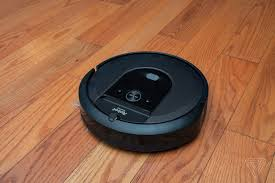
\includegraphics[width=0.47\textwidth]{Img/Roomba}}}%
    \qquad
    \subfloat[Ejemplo del recorrido de un robot aspiradora comercial]{{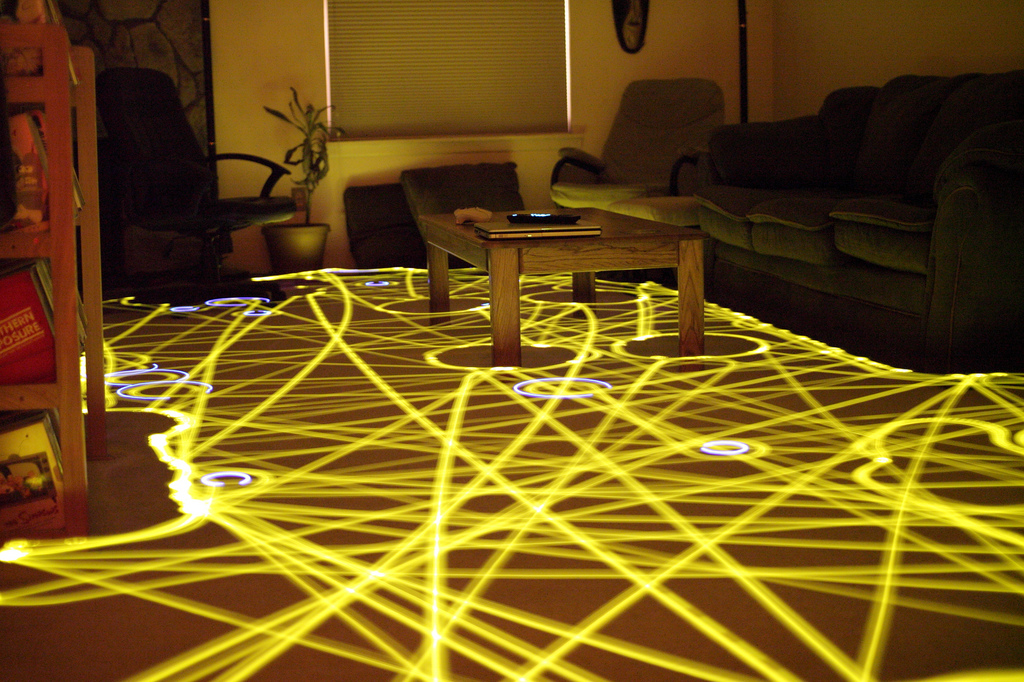
\includegraphics[width=0.47\textwidth]{Img/VaccumRobot.png}}}%
    \caption{El robot aspiradora}
    \label{fig:vaccumrobot}
\end{figure}

\ifimagenes
Si lo que se pretende es optimizar el recorrido del robot, la
\else
A pesar de que se busque reducir la interacción humana bajo estas circunstancias, no todos los robots hoy en día son autónomos, principalmente debido a la falta de robustez del algoritmo de control involucrado en el proceso. Tomando por caso el ejemplo anterior, si bien el robot aspiradora es autónomo, su eficiencia respecto a la forma óptima de realizar la tarea no es una garantía en todos los casos.

Es útil distinguir entre robots que están inmóviles, como un brazo robótico en una fábrica, y robots que son móviles, como un auto sin conductor. En este trabajo se hará hincapié en los robots móviles. Usamos este término para describir un robot impulsado por sus propios medios que puede moverse cinemáticamente entre ubicaciones en su entorno. A su vez, cuando se habla de la posición y orientación combinadas del robot, esto se define como su \textit{pose}.

Los robots móviles pueden referirse a robots que se mueven sobre el suelo, bajo el agua, a través del aire y en entornos de microgravedad, tales como los que pueden observarse en la Figura \ref{fig:mobilerobots}. Si bien este trabajo busca aplicar en parte a cualquiera de estos entornos, el enfoque del mismo se refiere principalmente a los robots móviles que permanecen en contacto con el suelo. Cada uno de ellos presentan su propia terminología para definirlos y diferenciarlos del resto, por ejemplo, el término vehículos terrestres no tripulados o UGV (del inglés \textit{unmanned ground vehicles}) a menudo se usa más específicamente para describir robots móviles terrestres, mientras que el término vehículos aéreos no tripulados o UAV (del inglés \textit{unmanned aerieal vehicles}) refieren principalmente a los drones.

Los robots móviles se mueven a través de entornos grandes y potencialmente dinámicos, lo que hace que la percepción sea mucho más difícil que los robots industriales con entornos de trabajo limitados y parámetros operativos rígidos. Por lo tanto, los robots móviles requieren sensores adicionales, una mejor percepción y mayores grados de autonomía para operar en entornos del mundo real que cambian con frecuencia.


\begin{figure}%
    \centering
    \subfloat[Wheeled robot]{{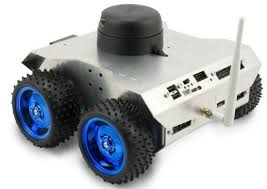
\includegraphics[width=0.25\linewidth]{Img/WheeledRobot.jpeg}}}%
    \qquad
    \subfloat[Legged robot]{{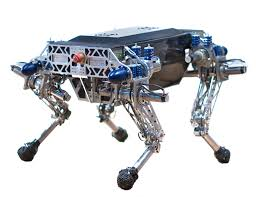
\includegraphics[width=0.25\linewidth]{Img/LeggedRobot.jpeg}}}%
    \qquad
    \subfloat[Tracked robot]{{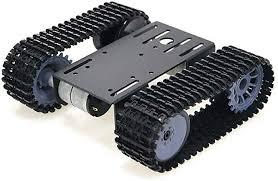
\includegraphics[width=0.25\linewidth]{Img/TrackedRobot.jpeg}}}%
    \qquad
    \subfloat[Drone]{{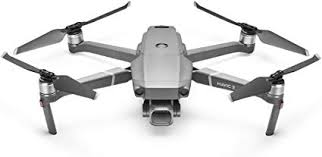
\includegraphics[width=0.3\linewidth]{Img/Drone.jpeg}}}%
    \qquad
    \subfloat[Water-based robot]{{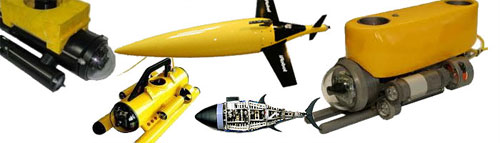
\includegraphics[width=0.5\linewidth]{Img/WaterBasedRobot.jpg}}}%
    \caption{Tipos de robot móviles}
    \label{fig:mobilerobots}
\end{figure}

Dentro de lo que respecta a robótica móvil, uno de sus desafíos actuales es lograr la completa autonomía del vehículo. Una gran parte de las empresas de la industria automotriz han dedicado mucho tiempo y dinero para lograr el objetivo. La investigación ha avanzado hasta el punto de que en la actualidad hay autos semi-autónomos disponibles en el mercado, y se cree ampliamente que en el futuro cercano casi todos los vehículos serán completamente autónomos. Para lograr esto, obviamente hay una necesidad de sensores y funciones avanzadas. Uno de los principales problemas es el hecho de que el vehículo debe ser consciente de su posición actual dentro de un entorno desconocido. Este proceso de determinar no solo su posición, sino también el mapa que lo rodea se conoce como la \textit{localización y mapeo simultáneos}, comúnmente abreviado como \textit{SLAM} (del inglés, \textit{simultaneous localization and mapping}).

El SLAM es un problema difícil de solucionar, así como lo fue para los humanos en el pasado. Tiempo atrás, los marineros usaban los llamados registros de fichas para estimar su velocidad y extrapolaban esta velocidad con el tiempo para calcular su pose. Este proceso de navegación por estima (en inglés, \textit{dead reckoning}) conduce inevitablemente a errores graves de posicionamiento con el tiempo y, por lo tanto, siempre se ha respaldado mediante el uso de puntos de referencia (o \textit{landmarks}) para la navegación. Quedándonos en este caso particular, con el uso de las estrellas los marineros lograban saber donde estaba el Norte, permitiendo corregir su dirección. Sin embargo, no siempre se podía observar este patrón por días debido al cielo nublado, entonces tenían que confiar solamente en su navegación por estima, haciendo que la incertidumbre crezca día tras día. Para el caso de los robots, cuando el mismo recorre un mapa completamente desconocido, acumulará error debido a las predicciones que debe tomar respecto a su pose y entorno en el que está, hasta el momento en que entra a un área con puntos de referencia conocidos, pudiendo así corregir su estimación de posición.

Volviendo al ejemplo del robot de limpieza, si el mismo conociera el mapa en el que se encuentra, podría entonces trazar la ruta mas óptima para realizar la limpieza del lugar. Como no todos los ambientes son iguales y cada uno tiene, por ejemplo, muebles ubicados en distintos lugares, dicho robot podría hacer primero un reconocimiento del lugar previo a la limpieza para tener una noción de todo el espacio, o bien obtener el mapa y la ubicación en la que se encuentra en base al movimiento que realiza, pasando por los lugares que le faltaron aspirar. Para cualquiera de las dos opciones, por lo tanto, necesitará tanto tomar los datos del lugar como controlar al vehículo para que vaya circulando por el ambiente.

La
\fi
estimación de la pose, entonces, es una parte no separable de aplicaciones como el control del vehículo y el mapeo. Varios sensores se utilizan comúnmente para estimar la pose de un robot. Las unidades de medición inercial (IMU), la cámara, la odometría de las ruedas\footnote{Se mide la rotación de las ruedas para estimar cambios de la posición del vehículo a lo largo del tiempo} para el caso de ciertos robots móviles y el LiDAR se encuentran entre los sensores más populares para la localización en interiores \cite{delrosario2016}, mientras que para exteriores suele sumarse el GPS a estos sensores, corrigiendo al mismo mediante acción de la IMU \cite{caron2006}.


\ifimagenes
\else
En la localización al aire libre, la señal del sistema de posicionamiento global (GPS) suele estar disponible y, dado que la posición se puede obtener con precisión mediante GPS, es la opción común para la fusión con los datos obtenidos de la IMU \cite{engel2014}. Sin embargo, en un entorno denegado por GPS, como dentro de un edificio, se deben usar otros sensores para corregir las estimaciones de la IMU. Un enfoque común para abordar este problema son la fusión IMU-cámara \cite{mirzaei2008}, \cite{hesch2009}, \cite{chambers2014}, \cite{hesch2013}, así como también el uso de LiDAR \cite{lee2016}.

Un algoritmo SLAM robusto es esencial para que cualquier robot móvil navegue de manera segura a través de un entorno no estructurado. El algoritmo SLAM con frecuencia define un marco de coordenadas global para que el robot opere; uno que generalmente es utilizado por todas las funcionalidades de alto nivel, como navegación, planificación de rutas, exploración, identificación de objetos, seguimiento de objetos y manipulación de los mismos. Estas dependencias hacen que el algoritmo SLAM sea una parte central de cualquier arquitectura de robot móvil, y las fallas irrecuperables son altamente indeseables. Es probable que cualquier robot desorientado por una falla de SLAM no pueda realizar su tarea, o peor, puede poner en peligro a los humanos, a sí mismo o al medio ambiente.

%Si bien se han demostrado varios algoritmos SLAM en laboratorios, es más difícil producir soluciones robustas en entornos no estructurados del mundo real. El deslizamiento de las ruedas, por ejemplo, puede producir mediciones de odometría ruidosas, mientras que los sensores del sistema de posicionamiento global (GPS) a menudo producen una localización global con saltos muy pronunciados para la misma posición. El SLAM robusto del mundo real se vuelve aún más difícil cuando estos errores de detección aleatorios y sistemáticos ocurren en entornos que tienen geometrías redundantes u objetos en movimiento. Por ejemplo, en el caso de los LIDAR bidimensionales, los algoritmos empleados con los mismos suelen presuponer que el robot se encuentra terrestre se encuentra sobre una superficie plana, tal como puede ser el cuarto de un hogar. Si la superficie presenta irregularidades muy marcadas, la tarea de mapeo en dos dimensiones del mismo aumentaría su complejidad, ya que no podría encontrar las relaciones entre los datos anteriores con los actuales (no coincidirían) por si solo, y dependería de sensores adicionales, como una IMU.

%Para poder realizar las tareas en tiempo real, es necesario contar con una capacidad de cómputo suficiente para no sólo adquirir todos los datos de los sensores, sino también procesarlos para conseguir el mapa junto a la pose en cada momento. En el presente trabajo, se desarrolla una plataforma de Hardware capaz de realizar dicha actividad, a su vez de describir dos algoritmos de SLAM, uno basado en la combinación de un LIDAR 2D junto a una IMU, y el otro basado en una cámara RGB-D, obteniendo entonces un SLAM tridimensional.
\fi



En particular, para el caso de la localización y mapeo tridimensional (SLAM 3D), los LIDAR 3D han adquirido bastante popularidad en el último tiempo con la llegada de los vehículos autónomos, aunque son muy costosos. Si se pretende entonces una opción más económica, las cámaras estéreo y RGB-D (\textit{D: Depth - profundidad}) son de las más utilizadas para esto, a su vez de poder obtener datos de color de las mismas. Los sensores RGB-D como la \textit{Microsoft Kinect} proporcionan directamente mapas de profundidad densos e imágenes en color. En general, los enfoques SLAM que operan en imágenes RGB-D son estructuralmente diferentes de los sistemas estéreo, ya que la entrada es RGB-D de profundidad en lugar de dos imágenes de color. A pesar de esto, pueden obtenerse nubes de puntos de profundidad a partir de ambos sensores con el procesamiento
\ifimagenes
\ifimagenespaper
adecuado, como los presentados por la librería OpenCV \cite{kaehler2017}.
\else
adecuado, lo cual se desarrolla en el apéndice.
\fi
\else
adecuado, como los presentados por la librería OpenCV \cite{kaehler2017}.
\fi

Una vez obtenidas las nubes de puntos de profundidad, una de las formas de calcular la posición y orientación del robot (conocido como la \textit{pose} del robot) a lo largo del tiempo es mediante la comparación entre dos nubes de puntos contiguas (una con los datos recientes y otra con los datos de la nube de puntos anterior), buscando en definitiva la transformación necesaria para que la nube de puntos actual pueda alinearse (o sea, que coincida lo mejor posible) con la nube de puntos anterior. Este proceso se lo conoce como el \textit{registro de la nube de puntos}, y suele llevar una serie de pasos, lo cual se desarrollará más adelante. Para poder facilitar el uso de nubes de puntos, existen librerías específicas para trabajar con dicha información, siendo algunas de ellas la \textit{Point Cloud Library} y \textit{Open3D}, las cuales implementan no sólo distintos algoritmos, sino también estructuras para facilitar el manejo de las nubes de puntos.

Si bien hay muchos robots móviles hoy en día en el mercado, gran parte de ellos son costosos, y sobre todo los que se encuentran equipados para realizar SLAM 3D. Para poder evaluar los algoritmos necesarios sin tener que ponerse en gasto, existen entornos de simulación pensados, entre otras cosas, para robots, consiguiendo resultados comparables con los reales. Unos de los más conocidos en el ámbito son \textit{V-REP} y \textit{Gazebo}, siendo este último el elegido para realizar el trabajo.

\subsection{Contribuciones}
En el presente trabajo, 
\ifimagenes
se desarrolla un algoritmo de registro de nube de puntos en base a los datos obtenidos de una cámara RGB-D en movimiento dentro de un ambiente estático, bajo el entorno de simulación Gazebo. En base a la transformación obtenida en cada iteración, se aplica la misma a la nube de puntos entrante, para luego sumarla al mapa 3D generado.

Como el trabajo presentado forma parte de una tesis de grado en desarrollo sobre SLAM 2D y 3D, se pretende que el mismo pueda fusionarse con los datos provenientes de otros sensores, en particular la IMU y el LIDAR 2D, para obtener una mejor estimación de la posición y, por consiguiente, obtener un mapa más exacto.

\else
se presenta una plataforma de Hardware capaz de realizar las tareas de SLAM que incluyen una gran cantidad de sensores, a su vez de contar la misma con un factor de forma de Hardware para que la misma pueda expandir sus funcionalidades en base a lo que requiera el usuario.

Luego, e describen dos algoritmos de SLAM, uno basado en la combinación de un LIDAR 2D junto a una IMU, y el otro basado en una cámara RGB-D, obteniendo entonces un SLAM tridimensional, ambos considerando un entorno estático. Debido a la falta de sensores capaces de brindar la información reuqerida, se realizaron las pruebas del mismo bajo el entorno de simulación Gazebo, con el fin de poder luego llevarlas a un escenario real cuando se tenga el robot completo.
\fi

A su vez, se provee de un código compatible con \textit{ROS}, un framework pensado para utilizar en robótica, permitiendo portabilidad y versatilidad a la hora de proporcionar los datos de los sensores, ya que el mismo utiliza un sistema de mensajes que permite vincular a dos procesos sin importar el método de adquisición o procesamiento de los datos, mientras los mismos respeten el tipo de mensaje en sí.

\subsection{Estructura del documento}
El presente documento se compone de las siguientes secciones
\ifimagenespaper
\else
y apéndices
\fi
\begin{itemize}
    \item \textbf{Introducción}: esta sección hace una breve introducción al SLAM, presentando los distintos sensores utilizados normalmente, a su vez de dar una primera aproximación al registro de nubes de puntos con los sensores RGB-D para realizar dicha tarea. A su vez, se mencionan las contribuciones realizadas.
    \ifimagenespaper
    \item \textbf{Marco teórico}:
    \else
    \item \textbf{Herramientas para el desarrollo de robots}: En esta sección se da una introducción al framework \textit{ROS}, en particular a su estructura y su modo de vinculación entre los distintos paquetes. Finalmente, se da una breve descripción de Gazebo.
        \ifimagenes
    \item \textbf{Marco teórico}:
        \else
    \item \textbf{Geometría tridimensional y marcos de referencia}: en esta sección se desarrollan los conceptos de la geometría tridimensional necesarias para abordar los temas del trabajo realizado, a su vez de mencionar distintos marcos de referencia usualmente utilizados.
    \item \textbf{Análisis de regresión}: en esta sección se desarrolla el denominado análisis de regresión, abarcando tanto la regresión lineal como la no lineal.
    \item \textbf{Estimación de estado}: siguiendo con el análisis de regresión, en esta sección se desarrollan distintos algoritmos de estimación de estado, siendo uno de los mas conocidos el filtro de Kalman.
    \item \textbf{Sensores}: en esta sección se mencionan distintos sensores utilizados comúnmente en lo que refiere al SLAM, a su vez de presentar distintos métodos de calibración de algunos de ellos y características importantes.
    \item \textbf{Simultaneous Localization And Mapping}: en esta sección se profundiza en lo que refiere al SLAM, mencionando no sólo distintos algoritmos que existen, sino también mencionando características importantes de la técnica en si.
    \item \textbf{Reconstrucción del entorno}:
        \fi
    \fi 
    en esta sección se describe tanto el flujo de trabajo del registro de nubes de puntos asi como también los distintos algoritmos utilizados comúnmente a la hora de realizarlo, asociando a los mismos con su implementación en la librería PCL. A su vez, se comenta como conseguir las nubes de puntos en base a los sensores utilizados comúnmente en este tipo de
    \ifimagenes
    aplicaciones, además de una calibración de los mismos.
    \item \textbf{Experimentos}: En base a la sección anterior, en esta se describe el flujo del algoritmo realizado, además de presentar los resultados obtenidos en base a la simulación realizada
    \else
    aplicaciones.
    \item \textbf{Plataformas disponibles}: en base a los sensores y datos necesarios, en esta sección se realiza un relevamiento de las distintas plataformas disponibles en el mercado, comparando cada una de ellas.
    \item \textbf{Resolución}: en esta sección se mencionan los métodos utilizados para lograr el objetivo del trabajo, basándose en las secciones anteriores. A su vez, se muestran los resultados obtenidos.
    \fi
    \item \textbf{Conclusiones}: En esta sección se desarrolla la finalidad conseguida del trabajo, evaluando distintos puntos de interés.
    \ifimagenes
    \item \textbf{Trabajos futuros}: en esta sección se mencionan distintos aspectos para lo que sigue luego de este trabajo.
    \else
    \item \textbf{Apéndices}: en esta sección se incluye información útil, como el esquemático de la placa realizada.
        \ifimagenespaper
        \else
    \item \textbf{Anexo}: Finalmente, se incluye un anexo con información útil a la hora de querer llevar a cabo una implementación con sensores físicos, utilizando los datos proporcionados por los mismos.
        \fi
    \fi
\end{itemize}

\subsection{Resumen}
En esta Sección se dio una introducción respecto a los temas que va a abordar el trabajo realizado, a su vez de mencionar las contribuciones por el mismo y, finalmente, mencionar las distintas secciones que se incluyen.
        \section{Marco teórico}
\label{sec:marcoteorico}
En esta sección se presentan distintos métodos para poder realizar una reconstrucción del entorno en base a las nubes de puntos, además de dar una introducción a la librería de nube de puntos (PCL) y su vínculo con ROS, utilizados para el desarrollo del trabajo.

\subsection{Reconstrucción del entorno}
En base a los datos provistos por los sensores exteroceptivos (LIDAR, cámaras, entre otros), el objetivo principal del trabajo consiste en recolectar dicha información para poder reconstruir el entorno en el cual se encuentra sumergido el robot, además de poder estimar su posición. Sin embargo, estos tipos de sensores proveen un campo de visión limitado, por lo que no es posible describir el mundo real como un todo en base a una sola medición de estos sensores, sino que solo puede mencionarse a una pequeña porción del mismo, denominada \textit{escena}.

A su vez, el tipo de dato que se tome de la escena dependerá del tipo de sensor extereoceptivo que los provea. Por ejemplo, una cámara monocular es capaz de otorgar imágenes 2D, mientras que con una cámara estéreo se consigue una nube de puntos 
\ifimagenes
\ifimagenespaper
tridimensional.
\else
tridimensional, tal como se describe en el apéndice.
\fi

\subsection{Point cloud}
Una \textit{nube de puntos}, o de su terminología en inglés, \textit{point cloud}, se utiliza para describir a un conjunto de puntos de datos en un espacio dado. Las nubes de puntos 3D, por ejemplo, se tratan de un conjunto de puntos tridimensionales que se caracterizan por tener principalmente cordenadas espaciales XYZ, y opcionalmente pueden dar información de intensidad, color, entre otras.

Como se mencionaba anteriormente, la nube de puntos de la escena adquirida dependerá del principio de medición del sensor utilizado. En concreto, puede categorizarse en: \cite{weinmann2016}
\begin{itemize}
    \item \textit{Técnicas pasivas}, donde la luz ambiental se encuentra presente, permitiendo utilizar sensores como cámaras estéreo para obtener las imágenes propias del entorno.
    \item \textit{Técnicas activas} donde los sensores emiten radiaciones electromagnéticas, tal como es el caso de los LIDAR o las cámaras infrarrojas.
\end{itemize}

Dependiendo de la técnica de adquisición involucrada y el dispositivo utilizado, los datos de la nube de puntos adquiridos pueden corromperse con más o menos ruido y, además de la información espacial en forma de coordenadas XYZ, los atributos de los puntos respectivos, como la información de color o intensidad también puede adquirirse, como se mencionaba anteriormente.

\subsection{Point Cloud Library (PCL)}
La \textit{Point Cloud Library (PCL)} se trata de un proyecto abierto desarrollado en \textit{C++} que ofrece herramientas para procesar imágenes o nubes de puntos tanto 2D como 3D. El framework PCL contiene numerosos algoritmos que realizan filtrado, estimación de características, reconstrucción de superficies, registro, ajuste de modelos y segmentación. Con estos métodos, es posible procesar la nube de puntos, extraer keypoints para reconocer objetos en el mundo en función de su apariencia geométrica, crear superficies a partir de las nubes de puntos y visualizarlas.

En general, PCL contiene una estructura de datos muy importante, que es $pcl::PointCloud$. Esta estructura de datos está diseñada como una clase de template que toma el tipo de punto que se utilizará como parámetro. Como resultado de esto, la clase de nube de puntos no es mucho más que un contenedor de puntos que incluye toda la información común requerida por todas las nubes de puntos independientemente de su tipo de punto. Algunos de los tipos de puntos más utilizados son
\begin{itemize}
    \item $pcl::PointXYZ$, el cual es el más simple que posee la librería, almacenando la información en XYZ únicamente
    \item $pcl::PointXYZRGB$, almacena además de la posición XYZ, el color en formato RGB de cada punto.
    \item $pcl::PointNormal$, representa la superficie normal en un punto dado y la medida de su curvatura, además de las coordenadas XYZ.
    \item $pcl::PointXYZI$, que a las coordenadas XYZ les asocia también información de intensidad del punto.
\end{itemize}

Debido al gran número de tipos de puntos que existen en la librería, cada algoritmo implementado en la misma refiere a una clase perteneciente a una jerarquía de clases con puntos en común específicos. Gracias a ello, dichos algoritmos pueden ser parametrizados en base a lo que necesite el usuario. 

\ifimagenes
\ifimagenespaper
\else
\subparagraph{Interfaz con ROS}
\fi
\fi
La interfaz PCL para ROS proporciona los medios necesarios para comunicar las estructuras de datos PCL a través del sistema de comunicación basado en mensajes proporcionado por ROS. Para hacerlo, hay varios tipos de mensajes definidos para contener nubes de puntos, así como otros productos de datos de los algoritmos PCL. En combinación con estos tipos de mensajes, también se proporciona un conjunto de funciones de conversión para convertir de tipos de datos PCL nativos en mensajes. Uno de los más importantes tipos de mensajes de ROS es el $sensor_msgs::PointCloud2$, el cual contiene una colección de puntos N-dimensionales, que pueden contener información adicional como normales, intensidad, entre otros.

Para relacionar ambos mundos, ROS cuenta con el paquete \textit{pcl\_conversions}\footnote{http://wiki.ros.org/pcl\_conversions}. Por ejemplo, en el Codigo \ref{lst:pc2pcl} se convierte un mensaje del tipo \lstinline{sensor_msgs::PointCloud2} a \lstinline{pcl::PointCloud<pcl::PointXYZRGB>}.

\begin{lstlisting}[caption=Conversión de mensaje ROS a PCL, label=lst:pc2pcl]
  // ROS PointCloud2
  sensor_msgs::PointCloud2 &pc2;
  
  // Output Cloud
  pcl::PointCloud<pcl::PointXYZRGB>::Ptr cloud_out(new pcl::PointCloud<pcl::PointXYZRGB>);
  // PCL PointCloud2
  pcl::PCLPointCloud2 pcl_pc2;   

  // Convert from ROS message to PCL data
  pcl_conversions::toPCL(pc2, pcl_pc2);
  pcl::fromPCLPointCloud2(pcl_pc2, *cloud_out);
\end{lstlisting}


\subsection{Adquisición de la nube de puntos}
Como se menciona en el documento, dependiendo del sensor utilizado para obtener los datos, se conseguirán las nubes de puntos asociadas dependiendo del principio de medición. A continuación se menciona en primera instancia una librería usada comúnmente en este tipo de aplicaciones (OpenCV), además de los sensores utilizados generalmente en este tipo de aplicaciones.

\subsubsection{OpenCV}
OpenCV\footnote{http://opencv.org} es una librería open source multiplataforma que busca brindar una infraestructura de visión artificial fácil de usar y que pueda utilizarse para aplicaciones de tiempo real, por lo que hace hincapié en la optimización. Para ello, OpenCV cuenta con un set de más de 500 funciones \cite{kaehler2017} que abarcan muchas áreas en visión, tales como calibración de cámaras, visión estéreo y robótica.

\subsubsection{Cámara estéreo}
Con el fin de poder simular el efecto de la percepción humana, las cámaras estéreo se ubican separadas una distancia fija y, por lo general, alineadas horizontalmente, como se observa la Bumblebee 2 en la Figura \ref{fig:stereoandrgbdcameras}.a. Al tener dos fuentes de imágenes distintas y ubicadas en una posición relativa conocida, es posible a partir de las mismas determinar la profundidad en la que se encuentran los objetos que ven entre ambas. 

Si bien se puede realizar con una cámara monocular, la técnica cuenta con mayor complejidad y con ciertas restricciones\footnote{Por ejemplo, sería necesario conocer una cierta cantidad de puntos claves del objeto para que, estando el mismo en una pose distinta a la analizada a priori, sea posible determinar la pose del objeto mediante estos puntos claves.}, aunque puede solventarse mediante el agregado de sensores que utilicen otro principio de medición\footnote{Las cámaras RGB-D, por ejemplo, cuentan con una cámara y sensores de distancia para determinar la ubicación de determinados píxeles.}.

Para poder conseguir una nube de puntos mediante el uso de dos cámaras, deben seguirse una serie de pasos \cite{kaehler2017}
\begin{enumerate}
    \item \textit{Remover las distorsiones} de la lente.
    \item Ajustar las distancias y ángulos entre las cámaras, conocido como \textit{rectificación}.
    \item Encontrar las mismas características en ambas cámaras, proceso conocido como \textit{correspondencia}. A partir de este se consigue un \textit{mapa de disparidad} (o \textit{disparity map}), donde las disparidades son las diferencias en la coordenada x de los planos de la imagen de la misma característica vista en las cámaras izquierda y dercha.
    \item Si se conoce el arreglo geométrico de las cámaras, puede cambiarse el mapa de disparidad en distancias por \textit{triangulación}. Este paso es denominado \textit{proyección}, y el resultado es un mapa de profundidad.
\end{enumerate}

Para obtener mejores resultados, es necesario que las cámaras estén sincronizadas entre sí, caso contrario los objetos en movimiento serán un problema.

\begin{figure}
    \centering
    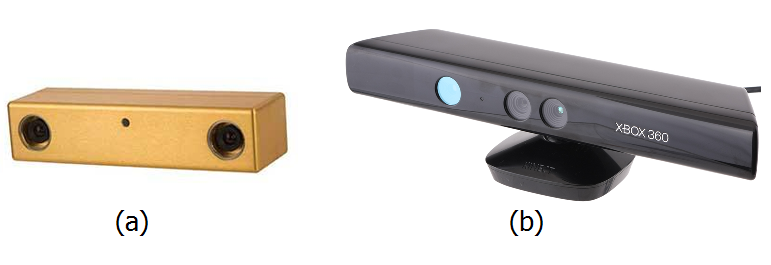
\includegraphics[width=.9\linewidth]{Img/bumblekinect}
    \caption{Cámaras: (a) Bumblebee 2, (b) Microsoft Kinect}
    \label{fig:stereoandrgbdcameras}
\end{figure}

\paragraph{Calibración}
La calibración estéreo depende de hallar la matriz de rotación y la traslación entre las dos cámaras previamente calibradas \cite{kaehler2017}, lo que puede realizarse mediante la función de OpenCV \texttt{cv::stereoCalibrate()}. En el mismo, se busca una sola matriz de rotación y un vector de traslación que relacione la cámara derecha con la cámara izquierda

Para la calibración en ROS se puede utilizar, al igual que en cámaras monoculares, el paquete \texttt{camera\_calibration}, el cual en este caso recibirá parámetros distintos. La interfaz gráfica para la calibración será similar al de cámaras monoculares, con la diferencia que en este caso aparecen ambas cámaras, aunque el principio de calibración del lado usuario es prácticamente el mismo, teniendo en cuenta que ahora en ambas cámaras debe visualizarse el patrón buscado, tal como se observa en la Figura \ref{fig:stereocalibrationchessboardrosexample}.
\begin{figure}
    \centering
    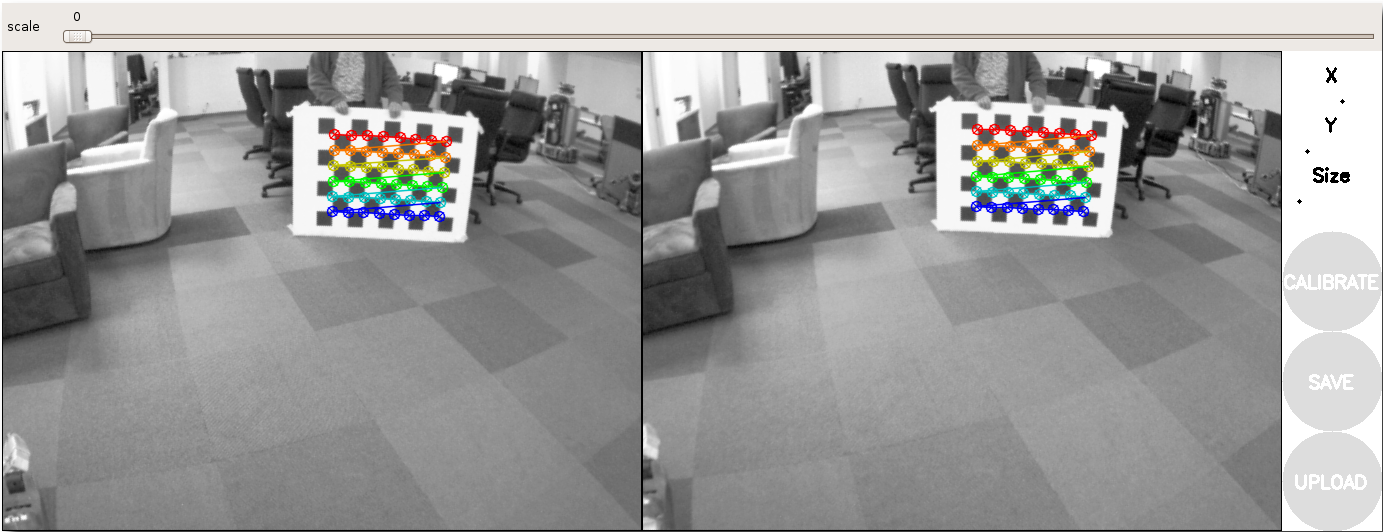
\includegraphics[width=\linewidth]{Img/StereoCalibrationChessboard.png}
    \caption{Calibración estéreo mediante ROS}
    \label{fig:stereocalibrationchessboardrosexample}
\end{figure}


\paragraph{Rectificación estéreo}
Si los planos de ambas cámaras no se encuentran perfectamente alineados, la disparidad estéreo aumenta su complejidad. Para poder mitigar este problema, lo que se busca es reproyectar los planos de la imagen de ambas cámaras para que residan en el mismo plano, conocido como \textit{rectificación estéreo}. Dentro de OpenCV, existen numerosas formas de obtenerlo, como pueden ser los algoritmos de Hartley o de Bouguet. El algoritmo de Hartley permite evitar la calibración de la cámara, en cambio para el segundo es necesaria.

Una vez que se obtienen los términos de la calibración estéreo, se pueden calcular los mapas de rectificación izquierda y derecha por separado utilizando para cada uno \texttt{cv::initUndistortRectifyMap()}.

En ROS, el paquete utilizado para dicha tarea es el denominado \texttt{stereo\_image\_proc}\footnote{\url{http://wiki.ros.org/stereo_image_proc}}, que permite obtener un mapa de profundidades. 

\paragraph{Correspondencia estéreo}
La correspondencia estéreo, esto es, coincidir un punto tridimensional en las vistas de ambas cámaras, requiere que estos puntos de ambas cámaras se solapen. Para ello, OpenCV implementa dos algoritmos distintos para correspondencias, convirtiendo dos imágenes (izquierda y derecha) en una sola imagen de profundidad
\begin{itemize}
    \item \textit{Block matching (BM) algorithm}, implementada mediante \texttt{cv::StereoBM()}, el cual es rápido y efectivo, aunque en escenas de baja textura presenta problemas. 
    \item \textit{Semi-global block matching (SGBM)}, implementada mediante \texttt{cv::StereoSGBM()}, el cual presenta una mayor exactitud que el BM, pero es computacionalmente más demandante.
\end{itemize}

En base a este proceso es que puede obtenerse una \textbf{nube de puntos} del entorno.

Para el caso de ROS, dentro del paquete \texttt{stereo\_image\_proc} se encuentra el ejecutable \texttt{dynamic\_reconfigure}\footnote{\url{http://wiki.ros.org/stereo_image_proc/Tutorials/ChoosingGoodStereoParameters}}, que permite modificar dinámicamente los parámetros de correspondencia, además de elegir el algoritmo a utilizar mediante una interfaz gráfica.

\subsubsection{Cámara RGB-D}
Las cámaras RGB-D\cite{hogman2011} en lugar de poseer dos cámaras monoculares presentan una cámara monocular con la ayuda de sensores infrarrojos para determinar la ubicación de determinados píxeles, siendo un ejemplo conocido de las mismas es la Microsoft Kinect, la cual se observa en la Figura \ref{fig:stereoandrgbdcameras}.b. Para que el mismo pueda obtener la nube de puntos, primero el sensor de distancia proyecta un patrón de moteado infrarrojo. El patrón proyectado es luego capturado por una cámara de infrarrojos en el sensor y comparado parte por parte con patrones de referencia almacenados en el dispositivo. Estos patrones fueron capturados previamente a profundidades conocidas en el proceso de calibración de los mismos. A continuación, el sensor estima la profundidad por píxel en función de los patrones de referencia con los que el patrón proyectado coincide mejor. Los datos de profundidad proporcionados por el sensor de infrarrojos se correlacionan luego con una cámara RGB calibrada. Esto produce una imagen RGB con una profundidad asociada a cada píxel. Una representación unificada popular de estos datos es una nube de puntos: una colección de puntos en un espacio tridimensional, donde cada punto puede tener características adicionales asociadas. Con un sensor RGB-D, el color puede ser una de esas características. Además, las normales de superficie aproximadas también se almacenan a menudo con cada punto en la nube de puntos resultante.

\subsection{Point cloud registration}
Si bien un primer paso es obtener la nube de puntos en base al sensor utilizado, uno de los principales enfoques utilizados en robots móviles con los mismos es el llamado \textit{registro de nube de puntos} o, de su terminología en inglés, \textit{point cloud registration}. Dicho proceso responde a encontrar una transformación espacial que alinee dos nubes de puntos generalmente contiguas en el tiempo.

En concreto, dada una nube de puntos fuente (tambíen llamada \textit{input} o \textit{source}) $P$ con puntos $p \in P$, y una nube de puntos objetivo $Q$ (llamada \textit{target}) con puntos $q \in Q$, el problema del registro se basa en encontrar correspondencias entre $P$ y $Q$, y estimar una transformación $T$ que, cuando se aplica a $P$, se alinea todos los pares de puntos correspondientes ($p_i \in P$, $q_j \in Q$). Un problema fundamental del registro es que estas correspondencias generalmente no se conocen y deben ser determinadas por el algoritmo de registro. Dadas las correspondencias correctas, hay diferentes formas de calcular la transformación óptima con respecto a la métrica de error utilizada, como se detalla a continuación.

El registro de dos nubes de puntos puede dividirse en una serie de pasos, los cuales se observan en la Figura \ref{fig:registrationpipeline} y conforman el denominado \textit{registration pipeline}. El mismo si bien puede extenderse para un caso más general \cite{garcia2017}, en este caso se da una estructura representativa del trabajo presente, siendo dichos pasos la \textit{selección}, \textit{matcheo}, \textit{rejection} y \textit{alineación}.

\begin{figure}[!ht]
    \centering
    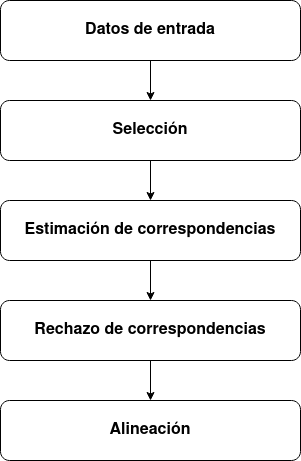
\includegraphics[width=0.45\linewidth]{Img/3DRegistrationPipeline.png}
    \caption{Registration pipeline}
    \label{fig:registrationpipeline}
\end{figure}

En primera instancia, debido a la gran densidad de puntos que presentan las nubes de puntos, además del ruido inherente de los sensores utilizados, es necesario realizar un proceso de \textit{selección} de los datos de interés, no solo para que el \textit{proceso de registro} pueda converger al valor óptimo, sino también para reducir el tiempo que tarda el algoritmo en completar el procesamiento.

Una vez que se tienen los datos seleccionados de cada una de las nubes de puntos a alinear, es necesario encontrar las correspondencias entre las mismas, esto es, encontrar un conjunto de puntos (los cuales suelen ser los \textit{keypoints}) en la nube de puntos fuente que se pueden \textit{identificar como los mismos puntos} en la nube de puntos objetivo.

En el proceso descripto anteriormente, normalmente una gran proporción de las correspondencias consideradas como tales en realidad son desajustes debidos al cambio de punto de vista, oclusión \cite{barazzetti2018}, entre otros. Estos desajustes suelen ser suficientes para arruinar los métodos de estimación tradicionales. Por lo tanto, es necesario eliminar o reducir la influencia indebida de los desajustes. Por ello, luego del pareo de los puntos característicos es necesario \textit{rechazar} las correspondencias para reducir el número de valores atípicos.

Finalmente, con las correspondencias filtradas, se busca la transformación que se ajusta mejor a ambas nubes de puntos mediante un proceso conocido como \textit{alineación}.

\ifimagenes
\else
%% VA O NO VA?????
A partir de la clasificación anterior, pueden diferenciarse dos tipos de algoritmos de registro, el \textit{registro basado en características (features)}, y los \textit{algoritmos de registro iterativos}, que se observan en la Figura \ref{fig:registrationprocess} y se detallan a continuación.
\begin{itemize}
    \item \textit{Registro basado en características (features)}, para calcular alineaciones iniciales, y
    \item \textit{Algoritmos de registro iterativos}, siguiendo el principio del algoritmo ICP para iterativamente registrar nube de puntos (que ya se encuentran relativamente alineadas).
\end{itemize}

\begin{figure}[!ht]
    \centering
    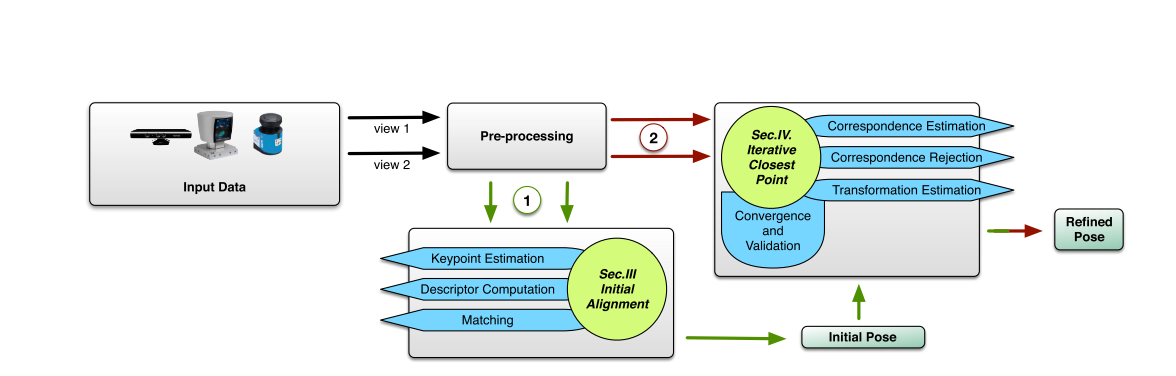
\includegraphics[width=\linewidth]{Img/RegistrationProcess.png}
    \caption{Registration process}
    \label{fig:registrationprocess}
\end{figure}

Para el registro basado en características, los descriptores de características geométricas se calculan y combinan en algún espacio de alta dimensión. Cuanto más descriptivos, únicos y persistentes sean estos descriptores, mayor será la probabilidad de que todas las \textit{coincidencias} (o \textit{correspondencias}) encontradas sean pares de puntos que realmente se correspondan entre sí.

En el algoritmo ICP de Besl y McKay \cite{besl1992} no se calculan descriptores de características, sino que se considera que los puntos más cercanos en el espacio cartesiano se corresponden entre sí. Se estima una transformación que minimiza las distancias euclidianas entre pares encontrados de puntos más cercanos en el sentido de mínimos cuadrados. El proceso de determinar los puntos correspondientes en los dos conjuntos de datos y calcular la transformación que los alinea se repite iterativamente. Se espera que el conjunto de puntos de origen converja hacia el conjunto de destino a medida que las correspondencias sean cada vez mejores. Simultáneamente, Chen y Medioni \cite{chen1992} formularon un algoritmo similar, pero en lugar de minimizar las distancias euclidianas al cuadrado entre los puntos correspondientes, aplicaron una métrica de error de punto a plano.
%%%%%
\fi
A continuación, se desarrollan los pasos nombrados anteriormente.

\subsubsection{Selección}
Como la información suele ser redundate y lo suficientemente densa como para necesitar un gran costo computacional a la hora de procesar los datos, es necesario filtrar las nubes de puntos quitando la información irrelevante, reduciendo así el tiempo de ejecución de los algoritmos. Si bien existen en la literatura muchos criterios para decidir cuales puntos tomar y cuales no, en principio se pueden distinguir dos métodos de reducción de datos, siendo el primero el de extraer automáticamente un pequeño conjunto de keypoints únicos y repetibles, mientras que el otro se basa en muestrear los datos originales con respecto a una distribución objetivo deseada. Mientras que el primero está destinado a la alineación inicial basada en características \cite{merino2016}, el segundo se puede utilizar para reducir de manera eficiente la cantidad de datos para los algoritmos de registro iterativos. PCL implementa varios de estos métodos de muestreo, en particular, el muestreo en el espacio índice (simplemente tomando cada n-ésimo punto), submuestreo uniforme en el espacio 3D de entrada (para capturar mejor las estructuras ambientales detectadas) y muestreo en el espacio de normales de superficie (para muestrear puntos en todas las orientaciones de la superficie). A continuación se presentan dos métodos que suelen emplearse en este tipo de tareas
\begin{itemize}
    \item \textit{Normal space sampling}: Al tratar generalmente con modelos suaves con pequeñas irregularidades (por ejemplo, un plano), el proceso puede resultar en el muestreo de muchos puntos que contienen esencialmente la misma información en términos de vectores normales. Por ello, la estrategia de \textit{normal space sampling} pretende dar uso a esta información \cite{rusinkiewicz2001}, y la misma consiste en, en primera instancia, agrupar puntos en ''cubos'' de acuerdo con los ángulos entre sus vectores normales (considerados en la esfera unitaria) y los ejes de coordenadas, y luego muestrear uniformemente sobre los cubos resultantes, proporcionando un submuestreo de los puntos con más vectores normales "frecuentes". Dentro de PCL, este algoritmo se encuentra implementado en el método \lstinline{pcl::NormalSpaceSampling}.
    \item \textit{Harris 3D}: El operador de Harris \cite{harris1988} se trata de un detector de puntos de interés para imágenes. El método es una técnica popular debido a su fuerte invariancia a la rotación, escala, variación de iluminación, y ruido de imagen \cite{schmid2000}. El detector de Harris se basa en la función de autocorrelación local de una señal, que mide los cambios locales de la señal con parches desplazados una pequeña cantidad en diferentes direcciones. El mismo se ha utilizado en muchas aplicaciones en procesamiento de imágenes y visión artificial por su sencillez y eficiencia. Sin embargo, el problema con los datos 3D es que la topología es arbitraria y no está claro cómo calcular las derivadas. Para solucionar este problema, en \cite{sipiran2011} proponen transformar a los puntos de la nube de la siguiente manera
    \begin{enumerate}
        \item Por cada punto de la nube, se define un \textit{punto vecino} del mismo, y se calcula el centroide de este último
        \item Todos los puntos de la nube se trasladan para que el centroide coincida con el origen de coordenadas
        \item Luego, se calcula un plano de ajuste a los puntos traslada
        \item Se aplica el \textit{análisis de componentes principales} (PCA de sus siglas en inglés) \cite{jollife2016} al conjunto de puntos y se elige el \textit{eigenvector} con el \textit{eigenvalue} asociado más bajo como la normal del plano de ajuste.
        \item Se rotan los puntos hasta que la normal al plano coincide con el eje z.
        \item El plano XY resultante se utiliza para calcular las derivadas. Estas derivadas se calculan utilizando una superficie cuadrática de seis términos (paraboloide) ajustada al conjunto de puntos transformados.
    \end{enumerate}
    Dentro de PCL, en el método \lstinline{pcl::HarrisKeypoint3D} se encuentra una implementación de dicho algoritmo.
\end{itemize}

\subsubsection{Estimación}
La estimación de correspondencias es el proceso de emparejar los puntos $p_i$ desde la nube de puntos fuente $P$ con sus vecinos más cercanos $q_j$ en la nube objetivo $Q$. 

En PCL, con la función \lstinline{pcl::registration::DetermineCorrespondences} se obtiene el conjunto de pares de correspondencia encontrados entre el la nubes de puntos fuente y objetivo. Cada par consta del índice del punto en la nube de origen y el índice de la coincidencia encontrada en la nube de puntos de destino. 

En el caso de datos de entrada provenientes de sensores que cumplen con el modelo de cámara estenopeica \cite{kaehler2017}, el procedimiento de estimación de correspondencia puede acelerarse significativamente con la contraparte de perder algo de precisión. Estos sensores incluyen cámaras RGB-D populares como Microsoft Kinect, y recopilan información del entorno en forma de imágenes de profundidad y color. En árboles PCL para búsquedas de vecinos más cercanos en el espacio 3D, es posible utilizar la naturaleza proyectiva de las imágenes de profundidad para obtener una aproximación razonable. Cada punto de la nube corresponde a un píxel en la imagen de profundidad, lo que permite proyecciones desde puntos de origen en coordenadas mundiales hasta el plano de la cámara del marco de destino mediante el uso de parámetros de cámara intrínsecos y extrínsecos. Este enfoque es rápido, pero impreciso para nubes de puntos con grandes discontinuidades de profundidad o para cuadros que están muy alejados entre sí. Es por eso que se recomienda usar este método solo después de que las dos nubes de puntos se hayan acercado, lo que lo hace bueno para alinear nubes de puntos consecutivas en una secuencia grabada a alta velocidad de cuadros.

%% QUE ONDA CON ESTO???
% Los métodos que extraen pocos keypoints pueden utilizar la fuerza bruta para encontrar correspondencias. Sin embargo, este proceso es computacionalmente costoso. Algunos métodos reducen el tiempo de cálculo minimizando el espacio de búsqueda, como 3D Shape Context [69] que preselecciona los posibles candidatos que satisfacen ciertos criterios y luego aplica fuerza bruta con estos candidatos. No obstante, en la mayoría de las situaciones, se necesitan algoritmos más elaborados para informar los resultados en un período de tiempo razonable.

% Como se necesitan al menos tres puntos no coplanares en cada conjunto para determinar una transformación rígida entre dos conjuntos de puntos 3D sin ambigüedad, el costo asintótico de tales enfoques está en O (n6). En consecuencia, el espacio para navegar en la búsqueda de correspondencias es enorme. Diseñar una estrategia de búsqueda sofisticada que sea capaz de aprovechar la información de detección y descripción tiene el potencial de reducir en gran medida los costos de cálculo y, por lo tanto, aumentar el rango de aplicación de tales algoritmos de registro. Los métodos existentes que implementan estrategias de búsqueda ya logran muy buenos resultados en comparación con los métodos típicos de fuerza bruta.

% A diferencia de los algoritmos de alineación, la finalidad de estas estrategias de coincidencia es lograr solo una alineación aproximada. La idea es identificar la posición arbitraria de las formas de entrada y encontrar las transformaciones entre ellas, lo más rápido posible. La precisión no es, por tanto, el factor más importante. En cambio, la robustez es clave proporcionando garantías para el posterior ajuste fino.
% A continuación se presentan algunos métodos conocidos de la literatura.

% \paragraph{Métodos basados en RANSAC}
% RANdom SAmple and Consesus (RANSAC) es un método iterativo diseñado para encontrar los parámetros de un modelo a partir de un conjunto de datos que contiene valores atípicos (\textit{outliers}). Dada una entrada de datos ruidosos, RANSAC encuentra los parámetros que ajustan los datos de entrada a un modelo dado, descartando los valores atípicos. Este enfoque es la base de una amplia variedad de métodos. Uno de ellos es el enfoque presentado por [34] que se basa en el hecho de que podemos determinar una transformación rígida con solo tres puntos (una base B). La idea es encontrar una base en una de las formas y encontrar la base correspondiente en la otra forma. El algoritmo funciona de la siguiente manera: 
% \begin{itemize}
%     \item primero, determina tres puntos diferentes al azar en la primera superficie: primario (ap), secundario (as) y auxiliar (aa). Considere que las distancias entre estos tres puntos son dps, dpa y dsa. Cada punto en la segunda superficie se considera como el punto correspondiente bp del punto primario ap en la primera superficie.
%     \item Luego, se busca la correspondencia del punto secundario en la segunda superficie a una distancia dps de bp. Si no existe ningún punto alrededor de bp a la distancia dps, descarte bp y comience de nuevo con otro punto primario en la segunda superficie. Sin embargo, si hay un punto secundario bs busque el punto auxiliar ba que satisface las distancias. La transformación entre ambas superficies se puede determinar cuando se identifica la base BB en la segunda superficie. Esta búsqueda se repite para todas las bases encontradas. La mejor transformación es la que tiene el mayor número de puntos correspondientes.
% \end{itemize}

% Aunque este método es robusto incluso con valores atípicos, el principal inconveniente es su tiempo de cálculo. De hecho, este método solo se puede utilizar con una pequeña cantidad de datos de entrada.

% Dentro de PCL, el método \lstinline{pcl::RandomSampleConsensus} representa una implementación del algoritmo RANSAC, tal como se describe en \textbf{[Fischler,1981]}.

% \paragraph{}
%%

%% VER SI PONER O QUE HACER







% \subsubsection{Decimación y filtrado}
% Uno de los grandes problemas que presentan las nubes de puntos al querer hacer un procesamiento de las mismas refieren a la gran densidad de puntos y al\usepackage{comment} ruido en si. Para el primer caso, por ejemplo, si se tiene una nube de 640x480 (estándar), se tendrían que procesar entonces 307200 puntos, generando que se requiera mucho tiempo para completar el procesamiento del algoritmo. El segundo problema, en cambio, genera que se malinterprete la información, provocando resultados incorrectos. 

\subsubsection{Rechazo}
Dado que las correspondencias no válidas pueden afectar negativamente los resultados del registro, la mayoría de los procesos de registro presentan un paso de rechazo. El mismo consiste en filtrar los pares de puntos emparejados en la etapa anterior para facilitar el algoritmo de estimación de la transformación hacia la convergencia al mínimo global. Este paso puede aprovechar la información auxiliar disponible de las nubes de puntos de entrada, como las normales de superficie locales o las estadísticas sobre las correspondencias. A continuación se detallan algunos de los algoritmos más utilizados
\begin{itemize}
    \item \textit{Rechazo de correspondencias basado en la distancia}: en base a un umbral, se filtran las correspondencias que estén a una distancia mayor que dicho límite. En PCL, se implementa mediante \lstinline{pcl::registration::CorrespondenceRejectorDistance}.
    \item \textit{Rechazo en base a la distancia mediana}: a diferencia del método anterior, en este caso el umbral se calcula en base a la mediana de todas las distancias punto a punto en las correspondencias estimadas inicialmente. Se utiliza la mediana ya que suele ser más efectiva en reducir la influencia de valores atípicos. El método \lstinline{pcl::registration::CorrespondenceRejectorMedianDistance} implementa dicha operación.
    \item \textit{Rechazo basado en RANSAC}: Este método aplica el RANdom SAmple Consensus \cite{fischler1981} para estimar una transformación para subconjuntos del conjunto dado de correspondencias y elimina las correspondencias atípicas basadas en la distancia euclidiana entre los puntos después de que la transformación calculada se aplica a la nube de puntos fuente. Es muy eficaz para evitar que el algoritmo ICP converja en mínimos locales, ya que siempre produce correspondencias ligeramente diferentes y es bueno para filtrar valores atípicos. Además, proporciona buenos parámetros iniciales para la estimación de la transformación con todas las correspondencias internas que siguen. El mismo cuenta con el método de PCL \lstinline{pcl::registration::CorrespondenceRejectorSampleConsensus}.
    \item \textit{Rechazo basado en la compatibilidad normal}: este filtro usa la información normal sobre los puntos y rechaza aquellos pares que tienen normales inconsistentes, es decir, el ángulo entre sus normales es mayor que un umbral dado. Puede rechazar pares erróneos que parecen correctos cuando se juzgan solo por la distancia entre los puntos. El mismo es implementado por \lstinline{pcl::registration::CorrespondenceRejectorSurfaceNormal}.
\end{itemize}

\subsubsection{Alineación}
A lo largo de los años, ha habido numerosos enfoques matemáticos para resolver la transformación rígida $T$ que minimiza el error de los pares de puntos. $T$ se compone de una rotación $R$ y una traslación $t$. Tenga en cuenta que, a continuación, cuando se hace referencia a una transformada $T$ y un punto $p$, se utilizarán coordenadas homogéneas. Hay dos métricas de error principales que se deben minimizar y que se han considerado en la literatura: \textit{punto a punto} (Ec. 2) y \textit{punto a plano} (Ec. 3), donde ($p_k$, $q_k$) es el \textit{k-ésimo} de el par $N$ corresponde desde la nube de origen a la nube de destino.
\begin{itemize}
    \item Métrica de error estándar de punto a punto: La métrica de error estándar utilizada en el algoritmo ICP es la métrica de error de punto a punto (Ec. 2). Fue mencionado por primera vez por Arun \cite{arun1987}; los investigadores propusieron varias formas de minimizarlo, seguidas de la introducción del algoritmo ICP \cite{besl1992}. Eggert y col. \cite{eggert1997} evaluó cada uno de estos métodos en términos de estabilidad numérica y precisión, llegando a la conclusión de que tienen un desempeño cercano. PCL ofrece una implementación (\lstinline{pcl::registration::TransformationEstimationSVD}) utilizando \textit{descomposición en valores singulares} (SVD), propuesto en primera instancia por \cite{horn1987}.
    \item \textit{Métrica de error de punto a plano}: Chen y Medioni \cite{chen1992} introdujeron la métrica de punto a plano (Ec. 3) y demostraron que es más estable y converge más rápido que los enfoques anteriores. Utiliza la distancia entre el punto de origen $\bm{p}_k$ y el plano descrito por el punto de destino $\bm{q}_k$ y su normal de superficie local $n_{\bm{q}_k}$. A diferencia de la métrica punto a punto, no tiene una solución de forma cerrada, por lo que la minimización se realiza con solucionadores no lineales (como Levenberg-Marquadt), o linealizándolo \cite{low2004} (bajo el supuesto de ángulos de rotación pequeños, es decir, $sin \theta \sim \theta$ y $cos \theta \sim 1$). Dependiendo de la superficie subyacente y la distribución de puntos, el uso de la métrica de error de punto a plano puede ser considerablemente más robusto. Un procedimiento estándar para minimizarlo se basa en el optimizador no lineal de Levenberg-Marquardt \cite{fitzgibbon2001}. Dicha funcionalidad se emplea en \lstinline{pcl::registration::TransformationEstimationPointToPlane}.
    \item \textit{Métrica de error punto-a-plano ponderada}: Asignar un peso diferente a cada correspondencia puede mejorar la convergencia. La ponderación de los pares de puntos puede verse como un rechazo de correspondencia suave, ajustando la influencia de los puntos correspondientes ruidosos en el proceso de minimización. La ponderación puede ser una función de la distancia punto a punto o punto a plano entre los puntos, una función del ángulo entre las normales correspondientes a los puntos, o una función del modelo de ruido del sensor que se ha usado. Un ejemplo de PCL puede ser \lstinline{pcl::registration::TransformationEstimationPointToPlaneWeighted}.
\end{itemize}


        \section{Experimentos}
\ifimagenes
A continuación, se presentan los experimentos realizados en base a los datos de una cámara estéreo que se dispuso físicamente, mencionando los inconvenientes de la misma para poder obtener los resultados esperados. Luego, se describe el pipeline utilizado para el registro de nube de puntos y, finalmente, se presentan los resultados obtenidos a partir de una simulación, mediante sets de datos previamente validados.
\else
\subsection{Plataforma de Hardware base desarrollada}
A partir del relevamiento realizado en la Sección \ref{sec:platforms}, se desarrolló la plataforma observada en la Figura \ref{fig:baseboardv2_1}, con el propósito de que la misma pueda utilizarse no sólo para la realización del trabajo, sino también para un gran número de aplicaciones dentro del area de la robótica. En el Apéndice \textbf{(MONGO)} puede encontrarse el esquemático completo del mismo.

\begin{figure}[!ht]
    \centering
    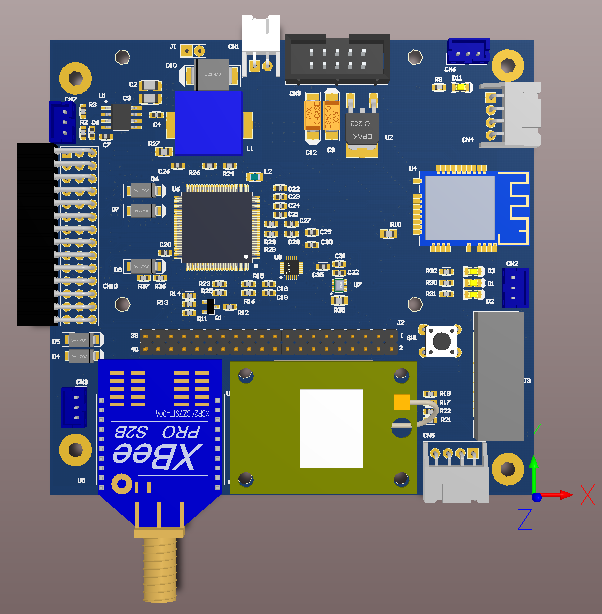
\includegraphics[width=\textwidth]{Img/BaseBoardV2_1.png}
    \caption{Plataforma base}
    \label{fig:baseboardv2_1}
\end{figure}

\subsubsection{Factor de forma}
En primer lugar, el tamaño de las plataformas suele ser un factor importante a la hora de querer conseguir una nueva. Por ello, los fabricantes generalmente siempre buscan tener el menor posible. Para este caso, como se hace hincapié en la versatilidad de la placa, se adopta el factor de forma PC104, en especial el PCIe104 OneBank, del cual se aprovechan las conectividades de SMBus y dos de USB. Debido a esto, el tamaño de la placa resulta ser de aproximadamente 10cmx10cm, haciendo que la placa no sea lo más pequeña posible, pero permitiendo entonces dicha versatilidad en base a un estándar ya definido.

\subsubsection{Alimentación}
Para poder alimentar la placa, el mismo permite hasta 18V de tensión de entrada, ya que cuenta con el regulador Buck sincrónico TPS54627\footnote{\url{http://www.ti.com/lit/ds/symlink/tps54627.pdf}}, el cual entrega una tensión de 5V y permite hasta 6A de corriente. De la salida del mismo se cuenta con un conector de alimentación para, por ejemplo, poder alimentar una Raspberry Pi sin necesidad de otra entrada de alimentación para la misma\footnote{Dichos microprocesadores suelen recomendar una alimentación de 3A promedio, el cual depende de los periféricos conectados a la misma, quedando en el peor de los casos 3A para el uso de la placa base en sí con todos sus perisféricos adicionales.}. Cabe destacar que, en caso que se tenga una Raspberry Pi montada en el conector pensado para la misma, en consecuencia no se podrá tener el una placa con factor de forma PC104 en la parte superior de la misma por temas de espaciado entre ellas.

\subsubsection{Unidad de procesamiento}
Si bien para el trabajo presente es necesario de un microprocesador para realizar tareas de alto rendimiento, tal como la recolección de imágenes de una cámara estéreo, en la presente se incluye como base un microcontrolador Cortex-M4, ya que el mismo está pensado para utilizarse en las tareas críticas del robot, como puede ser un control básico. Si bien para un robot terrestre esto puede no ser necesario, en el caso de querer realizar un drone, por ejemplo, la estabilidad del mismo al estar en vuelo es vital para evitar inconvenientes. En caso que se requiera mayor poder de cómputo, la placa cuenta cun una base para montar una Raspberry Pi compatible. Mas allá de que muchas de las plataformas vistas en la Sección \ref{sec:platforms} cuentan sólo con microprocesadores, se pretende en este caso aumentar la tolerancia a fallos al separar las tareas en dos unidades de procesamiento distintas, enfocando una de ellas a las tareas de control y funciones básicas, y la otra, por ejemplo, a realizar el SLAM.

\subsubsection{Conectividad}
Como se anticipó anteriormente, el mismo cuenta con el estándar de Hardware PCIe/104 OneBank, contando con comunicaciones de SMBus y USB por el mismo. Además de esto, el mismo dispone de conectores para
\begin{itemize}
    \item UART
    \item I2C
    \item GPIOs, además de salidas PWM con conectores propios pensadas para utilizar en distintos ESCs o controladores de motores
    \item Cuenta con pines específicos para montar una placa Raspberry Pi compatible, utilizando como medios de comunicaciones entre las mismas los protocolos UART e I2C.
\end{itemize}

\subsubsection{Sensores integrados}
Como existe una gran cantidad de sensores distintos dentro de las aplicaciones robóticas, en la placa base se montaron los más utilizados en las plataformas estudiadas en la Sección \ref{sec:platforms}.
\paragraph{Unidad de medición inercial (IMU)}
Siendo la IMU el sensor más utilizado dentro de la robótica aérea para el control del mismo, este sensor puede ser utilizado para un gran número de aplicaciones distintas, como por ejemplo para la corrección de la señal de GPS para calcular la posición del robot \textbf{(REF GPS IMU)}. Si bien existe una gran cantidad de IMUs distinta, tanto sea a nivel precio como en base a la cantidad de sensores que tengan (acelerómetro-giróscopo, acelerómetro-giróscopo-magnetómetro), dentro de la placa se dispone de una MPU9250\footnote{\url{https://invensense.tdk.com/wp-content/uploads/2015/02/PS-MPU-9250A-01-v1.1.pdf}}, la cual cuenta con nueve grados de libertad (9 \textit{degrees of freedom - DOF}), ya que posee un juego de acelerómetro, giróscopo y magnetómetro de tres ejes cada uno. Este integrado es una mejora del MPU6050, el cual se trata de un un giróscopo y un acelerómetro (6 DOF), resultando entonces en un \textit{multi-chip module} (MCM) de dos obleas, una correspondiente a un acelerómetro y un giróscopo, y la otra corresponde al magnetómetro AK8963. En concreto, las orientaciones de referencia de ambas obleas difieren, como puede verse en la Figura \ref{fig:mpu9250orientations}. Como se trata de un sensor de bajo costo, el mismo no suele tener todos sus sensores alineados correctamente.
\begin{figure}
    \centering
    \subfloat[Orientación de la oblea correspondiente al giróscopo  y el acelerómetro]{{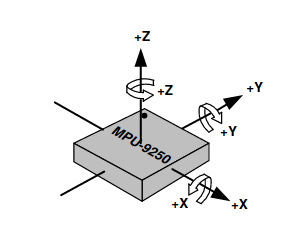
\includegraphics[width=0.45\textwidth]{Img/MPU9250GyroAccel.png}}}%
    \qquad
    \subfloat[Orientación de la oblea correspondiente al magnetómetro]{{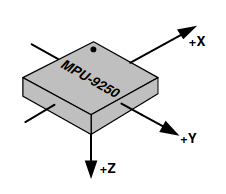
\includegraphics[width=0.45\textwidth]{Img/MPU9250Mag.png}}}%
    \caption{Orientaciones dentro del integrado MPU9250}
    \label{fig:mpu9250orientations}
\end{figure}

Generalmente, es recomendable que la IMU se encuentre en el centro de masa del robot. Sin embargo, debido a que la placa puede personalizarse con el agregado de módulos externos, se eligió el centro de coordenadas de la placa para la ubicación de la IMU.

\paragraph{Barómetro}
Si bien para el trabajo presentado puede no ser de utilidad, los barómetros son muy utilizados en los vehículos aéreos, ya que debido a las alturas elevadas que pueden alcanzar, el uso de un ultrasonido para medir la distancia al suelo sirve sólo para una corta distancia, mientras que los barómetros económicos son útiles a considerables alturas, siendo ambos métodos utilizados para tal fin. Al igual que el magnetómetro, la medición del barómetro respecta a una magnitud externa al robot, la presión atmosférica, y los datos del mismo suelen utilizarse en combinación con una IMU para conseguir una mejor estimación de la altitud\textbf{(Tanigawa, 2008)}, así como también para corregir la estimación de altitud del GPS\textbf{(Zaliva, 2014)}.

En concreto, para la placa se optó por el uso del barómetro BMP280\footnote{\url{https://cdn-shop.adafruit.com/datasheets/BST-BMP280-DS001-11.pdf}}, el cual es una mejora de su predecesor, el BMP180, aunque ambos tienen una precisión de aproximadamente un metro.

\paragraph{GPS}
Si bien el circuito integrado no se encuentra soldado en la placa base, en la misma se encuentra un soporte para poder colocar el módulo U-Blox GPS NEO6MV2, observada en la Figura \ref{fig:gpsneo6mv2}, el cual puede conseguirse fácilmente en el mercado local, aunque, como el resto de los sensores utilizados, presenta un error considerable en caso de que se quiera utilizarlo en soledad para calcular la posición global del robot, además de contar con una frecuencia de datos máxima de $1Hz$.
\begin{figure}
    \centering
    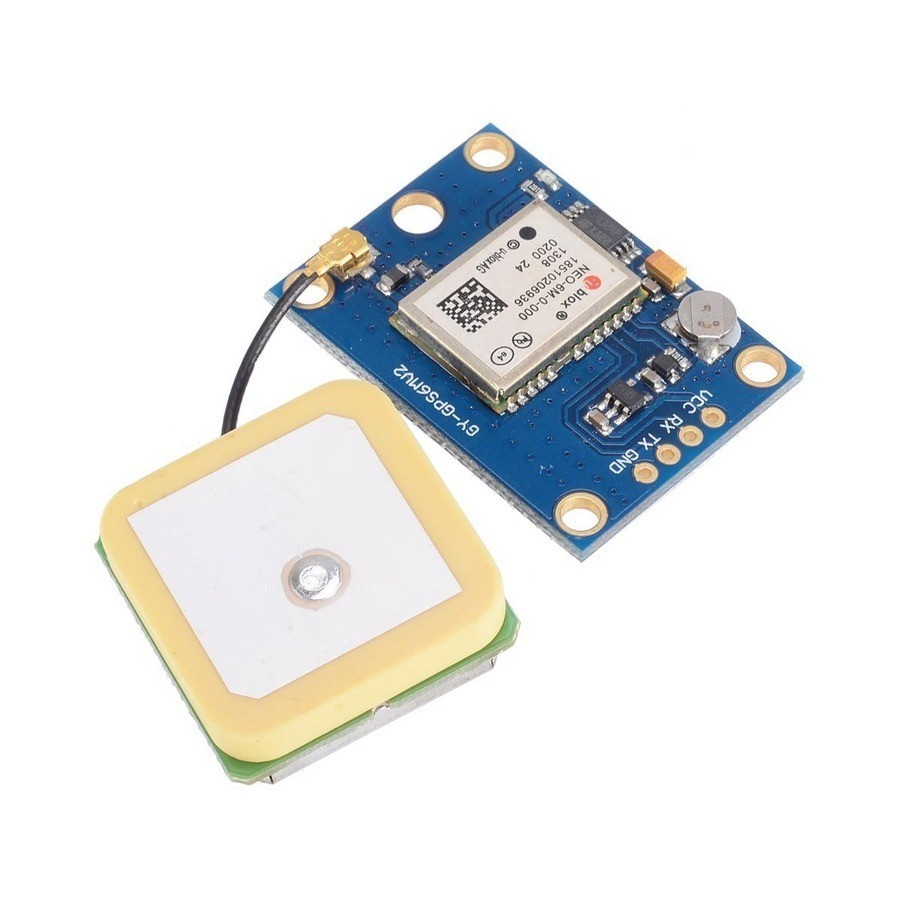
\includegraphics[scale=0.2]{Img/GPSNEO6MV2.jpg}
    \caption{Módulo U-Blox GPS NEO6MV2}
    \label{fig:gpsneo6mv2}
\end{figure}

\subsubsection{Sensores externos}
Si bien los sensores pueden agregarse mediante cualquiera de los pines de conectividad presentes en la placa, el mismo cuenta con la posibilidad de utilizar la interfaz DCMI, común en cámaras de baja resolución. Esto pude ser de utilidad en caso que se quiera tomar imágenes sólo con el uso del microcontrolador presente en la placa base.

Como gran parte de las aplicaciones robóticas cuentan con más de dos ultrasonidos, en la placa existen pines específicos para conectar hasta cinco de los mismos, ya que si bien la señal de Trigger para cada uno de los ultrasonidos es independiente, la señal de Echo es compartida, teniendo sólo que controlar un sólo pin, y en base a la señal de Trigger enviada puede conocerse cúal de ellos fue el que respondió. En caso que se requieran agregar más de estos sensores, puede hacerse utilizando los GPIOs disponibles.
\subsubsection{Sistemas de comunicaciones}
Para poder comunicar al robot, el mismo cuenta con
\begin{itemize}
    \item El módulo WiFi ATWINC1500\footnote{\url{http://ww1.microchip.com/downloads/en/DeviceDoc/ATWINC15x0-MR210xB-IEEE-802.11-b-g-n-SmartConnect-IoT-Module-Data-Sheet-DS70005304C.pdf}}, el cual es un módulo de bajo consumo bajo el estándar IEEE 802.11, conectado al microcontrolador mediante SPI.
    \item El módulo XBee-PRO S2C\footnote{\url{https://www.digi.com/resources/documentation/digidocs/pdfs/90002002.pdf}} mediante UART que, a diferencia del módulo WiFi, se trata de la versión Through-Hole, debido a la complicación que presentaba incluir su versión SMD y cumplir con los requisitos del estándar PC104.
    \item Al tener varios GPIOs disponibles, puede utilizarse un gran número de conectividades para radiocontrol (RC), tales como PPM y PWM. A su vez, se cuenta con la capacidad de incorporar un sistema Futaba S.Bus, ya que cuenta con un inversor de señal en una de sus entradas de UART. Sin embargo, para todos ellos es necesario agregar el receptor requerido.
\end{itemize}


\subsection{Robot desarrollado}
Antes de poder llegar al modelo final del robot, primero deben abordarse los aspectos considerados necesarios para la elaboración del mismo.

\subsubsection{Unidad de procesamiento}
Para que el robot pueda realizar tareas de SLAM, el mismo requiere de sensores exteroceptivos, en concreto de un LIDAR y una cámara estéreo, por lo que la unidad de procesamiento base (el Cortex-M4) no sería suficiente. Por ello, se adiciona al soporte específico del mismo una Raspberry Pi 4, buscando no sólo poder recolectar la información de estos sensores, sino también extender la capacidad de cómputo.

\subsubsection{Sensores útiles integrados en la plataforma base}
Como se pretende utilizar la placa base presentada anteriormente, ya que se busca realizar un robot terrestre, de la misma para el desarrollo de SLAM es de interés especialmente la IMU integrada en el mismo, dejando de lado el barómetro por no despegarse del piso. Si bien el GPS puede ser de gran utilidad para calcular la posición georeferenciada, se pretende poder realizar un \textit{SLAM indoor}, esto es, un SLAM dentro de un espacio cerrado, donde la señal de GPS se encuentra denegada.

\subsubsection{Módulos y sensores externos}
Como se mencionó anteriormente, en el robot se pretende utilizar un LIDAR y una cámara estéreo como sensores extereoceptivos. Como los mismos suelen ser costosos, se utilizaron provistos por la facultad, los cuales son
\begin{itemize}
    \item Scanse Sweep Laser Scanner\footnote{\url{https://s3.amazonaws.com/scanse/Sweep_user_manual.pdf}} (Figura \ref{fig:externalmodulesandsensors}.a): Se trata de un sensor LIDAR montado sobre una pieza giratoria, permitiendo entonces el sensado en 360 grados. Cuenta con una recolección de 1000 muestras por segundo, con un rango máximo de hasta 40 metros segun especificación. La frecuencia de escaneo máxima respecta a 10Hz.
    \item Minoru 3D Webcam\footnote{\url{https://www.robotshop.com/media/files/pdf/user-guide-3d-webcam.pdf}} (Figura \ref{fig:externalmodulesandsensors}.b): Se trata de una cámara estéreo, la cual se comunica mediante USB 2.0, presentando entonces un compromiso de resolución-marcos por segundo debido a la transferencia máxima del protocolo. Las cámaras no se encuentran sincronizadas, teniendo un desvío máximo de 16.5ms.
\end{itemize}
\begin{figure}
    \centering
    \subfloat[Scanse Sweep Laser Scanner]{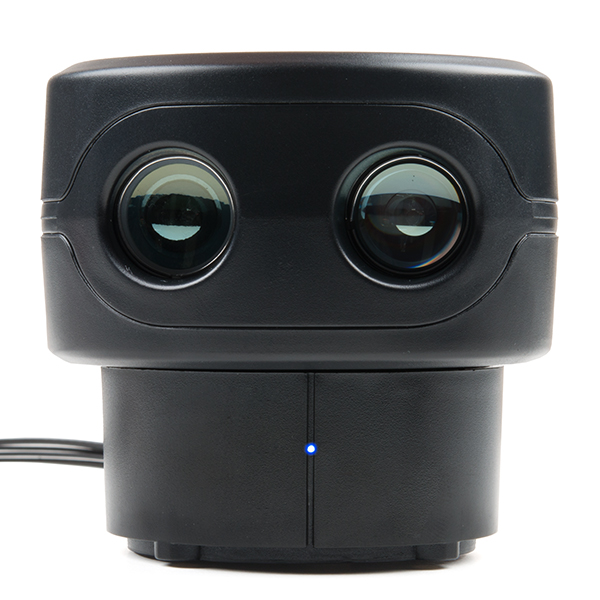
\includegraphics[width=0.2\textwidth]{Img/scanse-sweep.jpg}}
    \qquad
    \subfloat[Minoru Webcam]{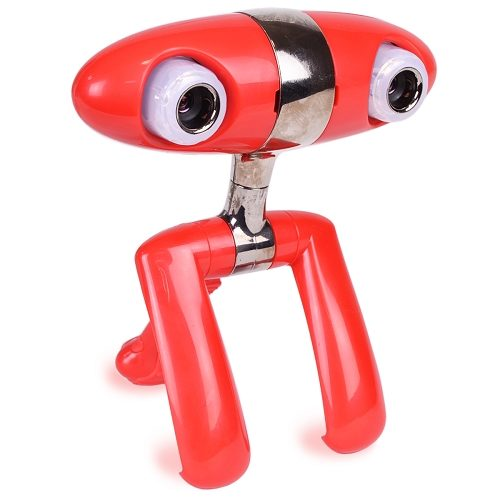
\includegraphics[width=0.2\textwidth]{Img/Minoru.jpeg}}
    \qquad
    \subfloat[Móudlo LM298]{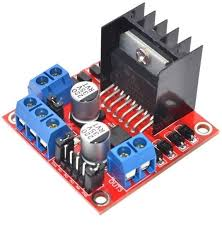
\includegraphics[width=0.2\textwidth]{Img/LM298.jpeg}}
    \qquad
    \subfloat[Móudlo LM2596]{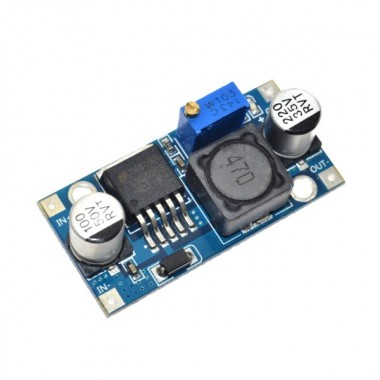
\includegraphics[width=0.22\textwidth]{Img/LM2596.jpeg}}
    \caption{Módulos y sensores externos}
    \label{fig:externalmodulesandsensors}
\end{figure}

Como es necesario poder controlar los motores, se incluyó un puente H para proveer a los mismos, utilizando el módulo comercial LM298, correspondiente a la Figura \ref{fig:externalmodulesandsensors}.c. Como la placa base proporciona una tensión regulada de 5V, para el puente H esto no es de gran utilidad, ya que el mismo requiere de 6 a 12V de alimentación. Para poder solucionar esto, se agregó también un módulo regulador del LM2596 ajustable, como el de la Figura \ref{fig:externalmodulesandsensors}.d.

\begin{figure}
    \centering
    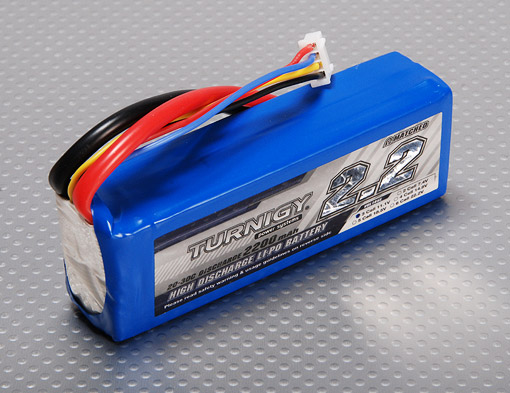
\includegraphics[width=0.5\textwidth]{Img/LiPo3S.jpg}
    \caption{Batería LiPo comercial utilizada en diferentes robots}
    \label{fig:lipobattery}
\end{figure}
\subsubsection{Estructura}
Siendo que tanto los sensores como la placa son relativamente voluminosos, es necesario que la estructura del robot permita ubicarlos a todos ellos sin estorbarse entre sí. Además de esto, al disponer de una batería LiPo de 3 celdas (Figura \ref{fig:lipobattery}), la misma debe tener un espacio dedicado no sólo para poder ubicarla, sino también que ofrezca algún tipo de resguardo, para evitar daños debido a efectos indeseados y corriendo el riesgo de que la misma pueda deteriorarse. Por estos motivo, se optó por el uso del chasis Auto Robot Smart Car 4WD, el cual cuenta con cuatro ruedas y motores, como se observa en la Figura \ref{fig:developedrobot}.a.
\begin{figure}
    \centering
    \subfloat[Chasis elegido para el robot terrestre]{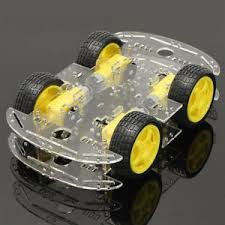
\includegraphics[width=0.45\textwidth]{Img/AutoRobotSmartCar4WD.jpeg}}
    \qquad
    \subfloat[Robot con piezas 3D montadas]{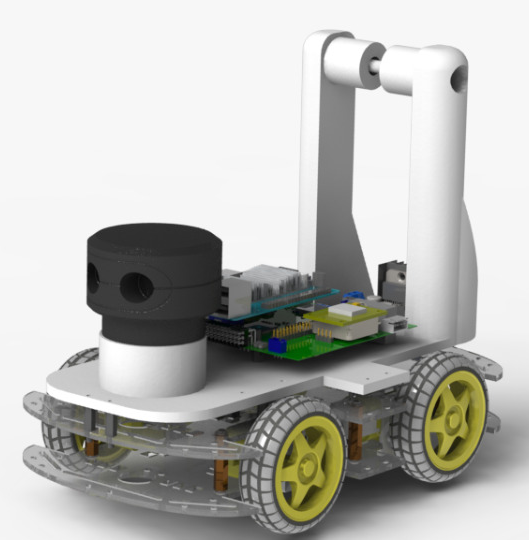
\includegraphics[width=0.45\textwidth]{Img/3DRobot.png}}
    \caption{Robot desarrollado}
    \label{fig:developedrobot}
\end{figure}

Para poder ubicar todos los componentes en la placa, es necesario que la cámara estéreo se encuentre distanciada del suelo, caso contrario dificultaría la triangulación debido al offset de cada una de las cámaras. A su vez, es preferible que el LIDAR tenga la menor cantidad de obstáculos posibles en el camino del láser, consiguiendo así una mayor cantidad de puntos útiles por barrido. A partir de esto, con el uso de una impresora 3D se desarrollaron piezas para cumplir con los requisitos, centrando la placa base en el centro del robot, tal como puede observarse en la Figura \ref{fig:developedrobot}.b. 





\subsection{Calibración de la unidad inercial de medición}
Para la calibración de la unidad inercial presente en el robot, esto es, el MPU9250, se realizó una base de madera fija, con el fin de poder moverlo con mayor facilidad. A su vez, como puede observarse en la Figura \ref{fig:baseboardimucalibrationwithframe}, se montó sobre la placa base una Raspberry Pi mediante el uso de \texttt{rosserial}, y se conectó esta Raspberry con la red WiFi para poder recolectar datos mediante ROS (guardándolos mediante el uso de \texttt{rosbag}), evitando el uso de cables externos, exceptuando al de alimentación.
\begin{figure}
    \centering
    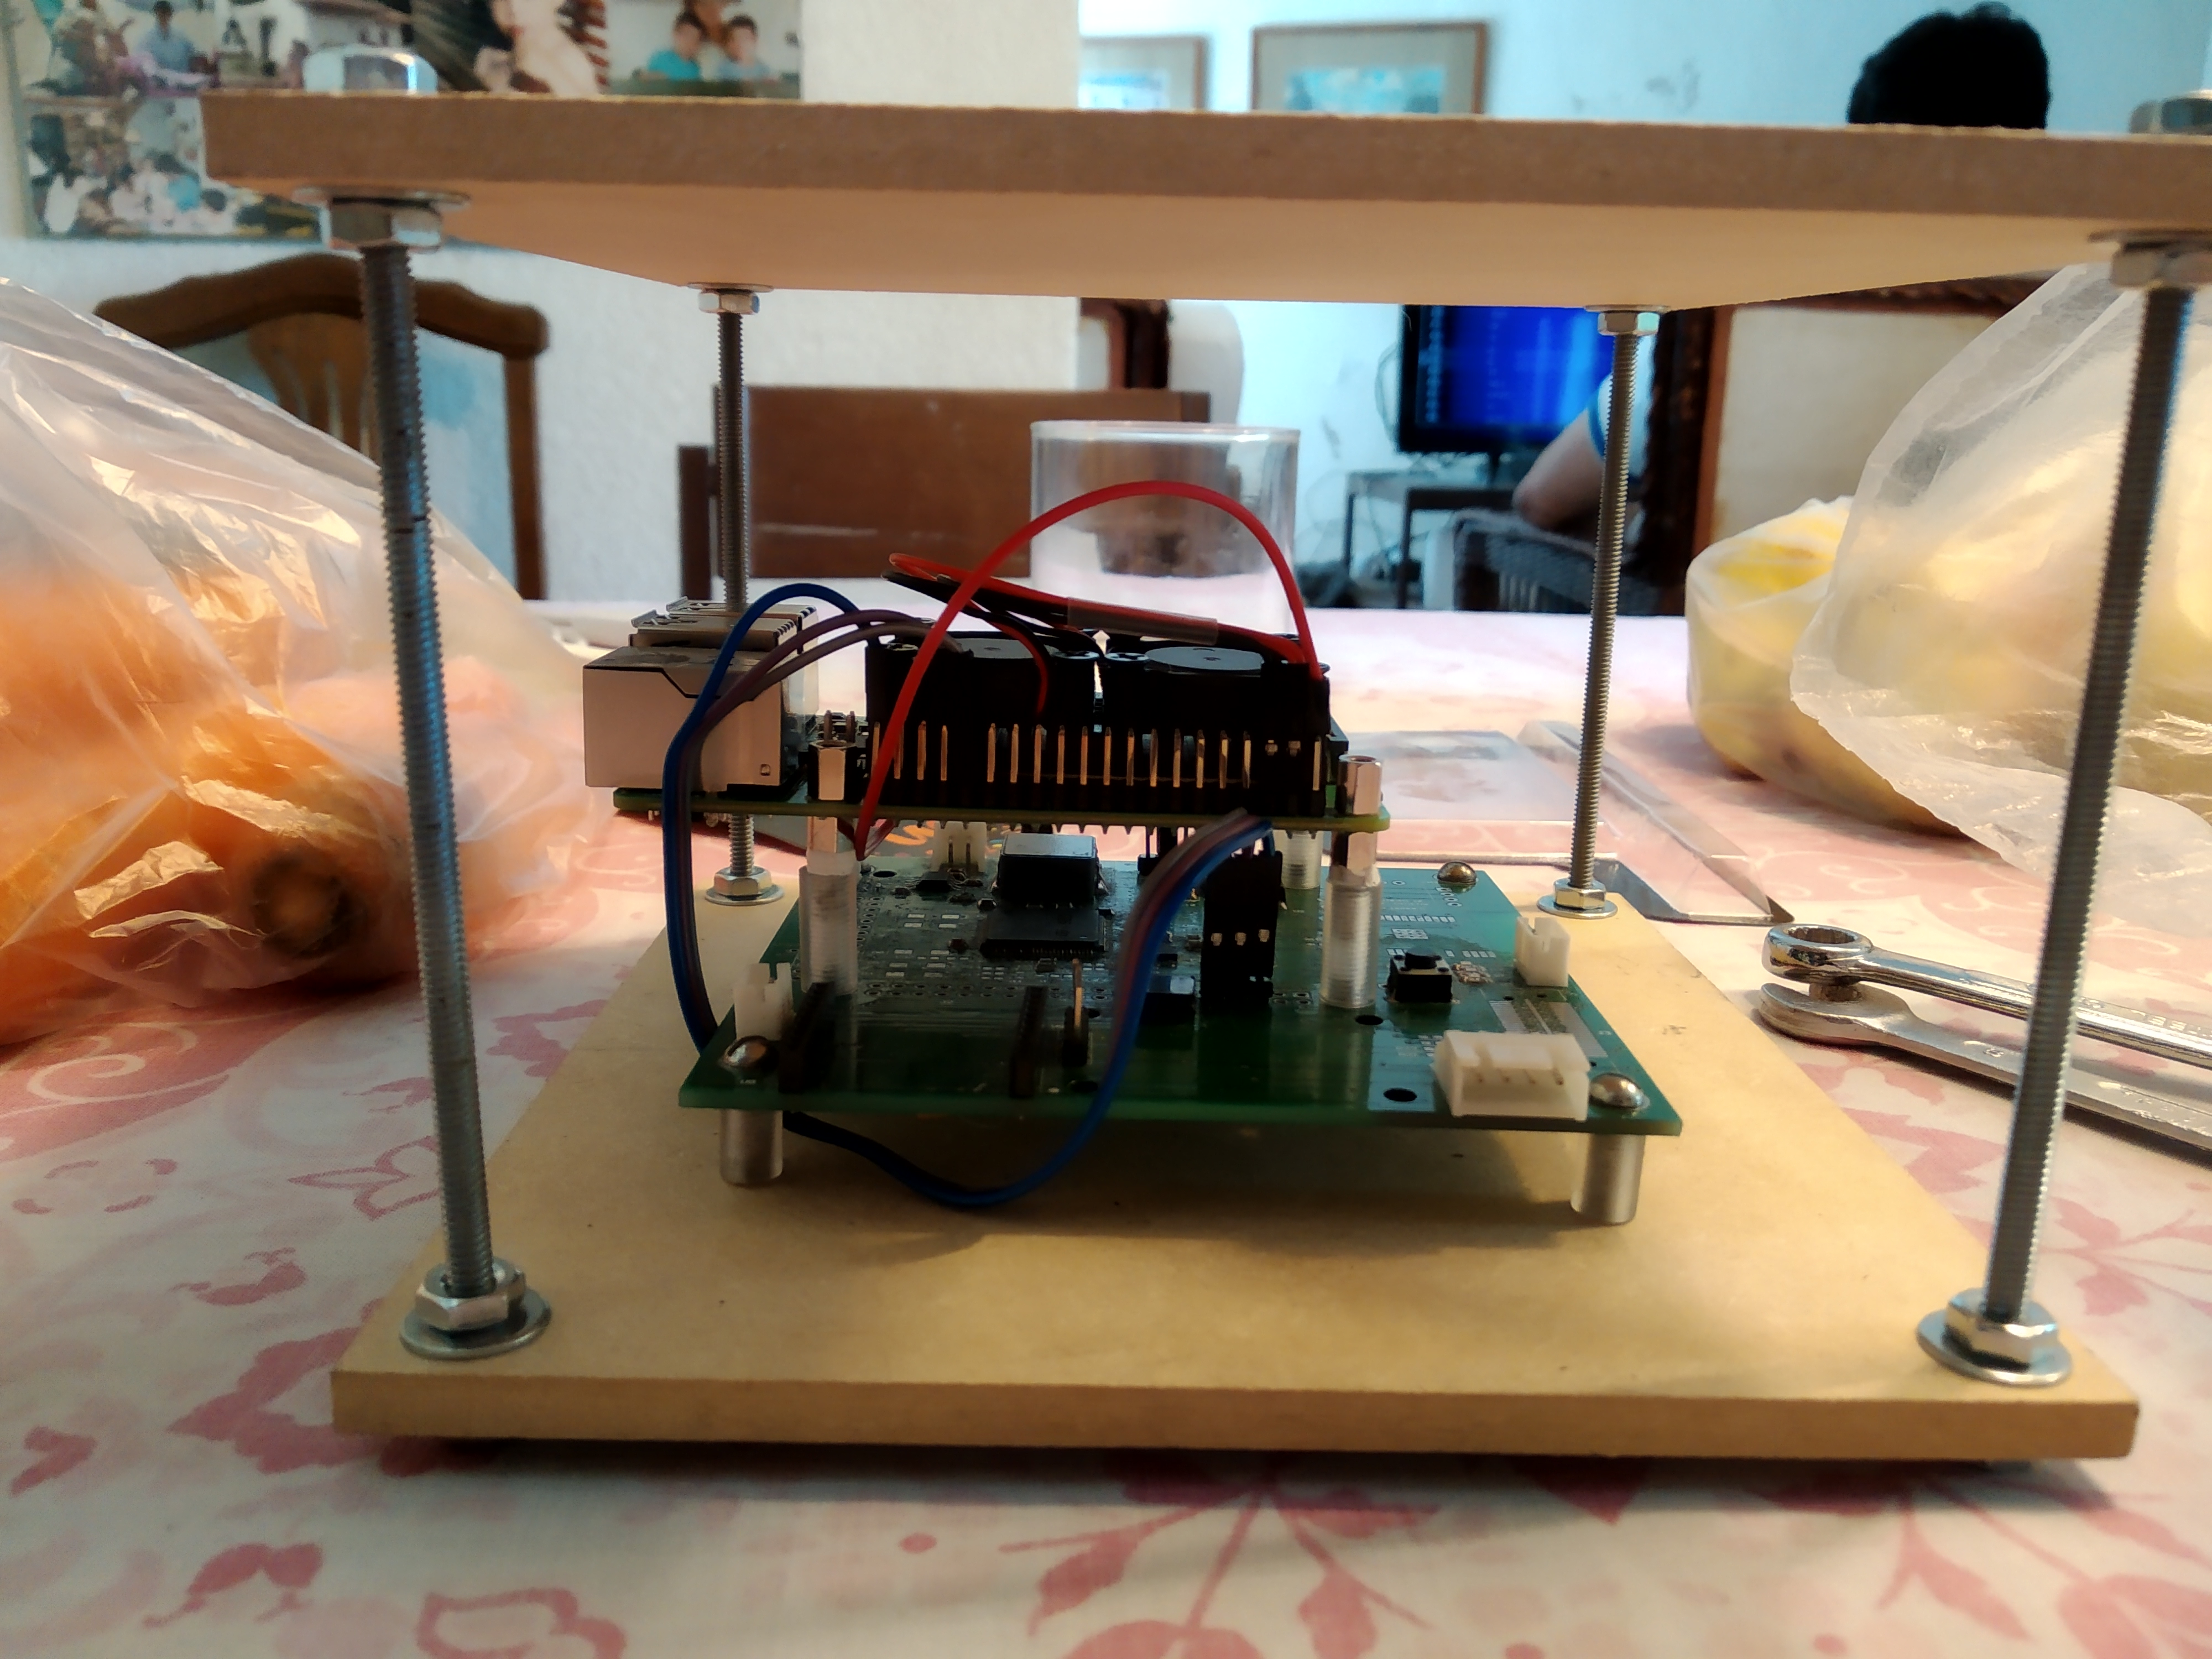
\includegraphics[width=\textwidth]{Img/BaseBoardIMUCalibrationWithFrame.jpg}
    \caption{Placa base con una Raspberry Pi sobre un marco fijo}
    \label{fig:baseboardimucalibrationwithframe}
\end{figure}


\subsubsection{Calibración del acelerómetro y giróscopo}
Tal como se desarrolló en la Sección \ref{sec:sensors}, la calibración del giróscopo se encuentra ligada a la calibración del acelerómetro, por lo que una mala calibración del acelerómetro hará llevará a una calibración inexacta del giróscopo. Además, como se pretende utilizar el mismo dataset para calibrar a ambos sensores, es necesario poder estimar todas las variables previas necesarias para tal fin.

\paragraph{Varianza de Allan para el cálculo de $T_{init}$}
Para poder conocer el tamaño adecuado que permita obtener el \textit{bias} del giróscopo en el instante inicial, se utiliza la \textit{varianza de Allan}[20][8] $\sigma_{Allan}$, la cual mide la varianza de la diferencia entre promedios de intervalos consecutivos, siendo entonces
\begin{align}
    \sigma_{Allan} &= \frac{1}{2} E[(x(\tilde{t},k) - x(\tilde{t},k-1))^2] \\
    &= \frac{1}{2K}\sum_{k=1}^K(x(\tilde{t},k) - x(\tilde{t},k-1))^2
\end{align}
donde $x(\tilde{t},k)$ es el \textit{k-ésimo} intervalo promedio que abarca $\tilde{t}$ segundos, y K es el número de intervalos en que se segmenta el tiempo total considerado. Se computa la varianza de Allan para los tres ejes del giróscopo, y en el intervalo de tiempo en el que los tres convergen a un valor pequeño representa una buena elección para elegir el período de inicialización, $T_{init}$.

Para el banco de ensayos presentado anteriormente, se tomaron mediciones de la unidad sin movimiento alguno pro un largo período de tiempo, obteniendo con la varianza de Allan las curvas de la Figura \ref{fig:imugyrovariance}. En la misma, puede observarse que un valor en el cual convergen las tres mediciones es alrededor de
\begin{equation}
    T_{init} = 8 s
\end{equation}
siendo este entonces el elegido.
\begin{figure}
    \centering
    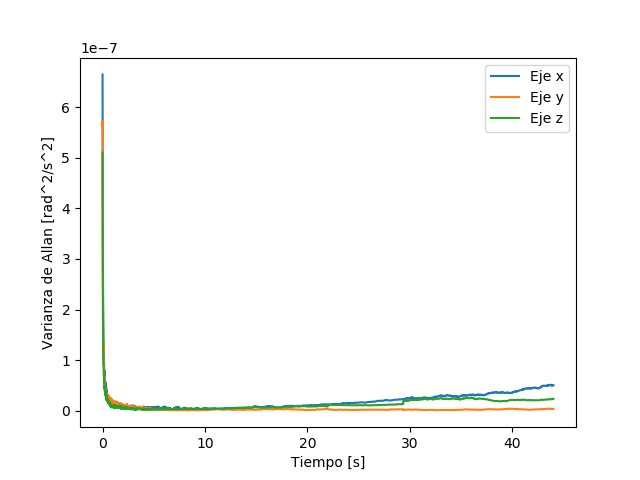
\includegraphics[width=\textwidth]{Img/IMUGyroVariance.png}
    \caption{Varianza de Allan para determinar el $T_{init}$ necesario para calcular el bias del giróscopo}
    \label{fig:imugyrovariance}
\end{figure}

\paragraph{Detector estático}
Como lo que se busca es promediar los datos del acelerómetro cuando el mismo permanece estático, es necesario poder entonces determinar en que momento el banco de pruebas se encuentra inmóvil. Tal como en \textbf{(Tedaldi, 2014)}, se propone el uso de un detector estático basado en la varianza de la aceleración, promediando cada un cierto tiempo $t_p$
\begin{equation}
    \xi(t) = \sqrt{(var_{t_p}\ a_x(t))^2 + (var_{t_p}\ a_y(t))^2 + (var_{t_p}\ a_z(t))^2}
\end{equation}
y luego compararlo con un cierto umbral para verificar de que se trate de un intervalo estático o no. Para ello, aprovechando el $T_{init}$ necesario en la calibración del giróscopo, se calcula primero un $\xi_{init}$ basado en el cálculo de la Expresión para el intervalo de tiempo mencionado, y luego, para cada instante de tiempo, si
\begin{equation}
     k\xi^2(t) < \xi^2_{init}
\end{equation}
el intervalo corresponderá a un estático, caso contrario se tratará de uno en movimiento. El parámetro $k$ se trata de un ajuste empírico para lograr mejores resultados.

Si bien el tiempo estático en que puede estar el banco para la calibración del acelerómetro puede ser extenso\footnote{Mientras más muestras se tengan, mejor será el promediado, aunque produce que se requiera más tiempo de procesamiento}, para el giróscopo es importante de que no alcance un tiempo mayor al expresado por la varianza de Allan, ya que indicaría que el mismo se encontraría en estado estacionario. Por ello, como se busca que el $T_init$ pueda ser expresado en base a los $t_p$ se adopta a este último con
\begin{equation}
    t_p = 1 s
\end{equation}

\paragraph{Calibración del acelerómetro}
En base a todos los parámetros calculados anteriormente, se tomaron las mediciones de la unidad inercial de medición, dejándola primero estática por aproximadamente $T_{init}$, y luego ubicándola en diferentes rotaciones con intervalos estáticos entre las mismas de menos de $T_{init}$. Como se tienen nueve parámetros para poder calibrar tanto el acelerómetro como el giróscopo (detallados en la Expresiones (\ref{eq:accelcalibrationparams}) y (\ref{eq:gyrocalibrationparams})\footnote{Mínimamente se necesitan la misma cantidad de mediciones que de incógnitas, aunque mientras más mediciones haya, mejor será la estimación}), se realizan un gran número de posiciones, obteniendo entonces las aceleraciones observadas en la Figura \ref{fig:imugyroaccelcal}. Junto a dichos datos, se representa el detector de estáticos, ajustado con un
\begin{equation}
    k = 2.0
\end{equation}
\begin{figure}
    \centering
    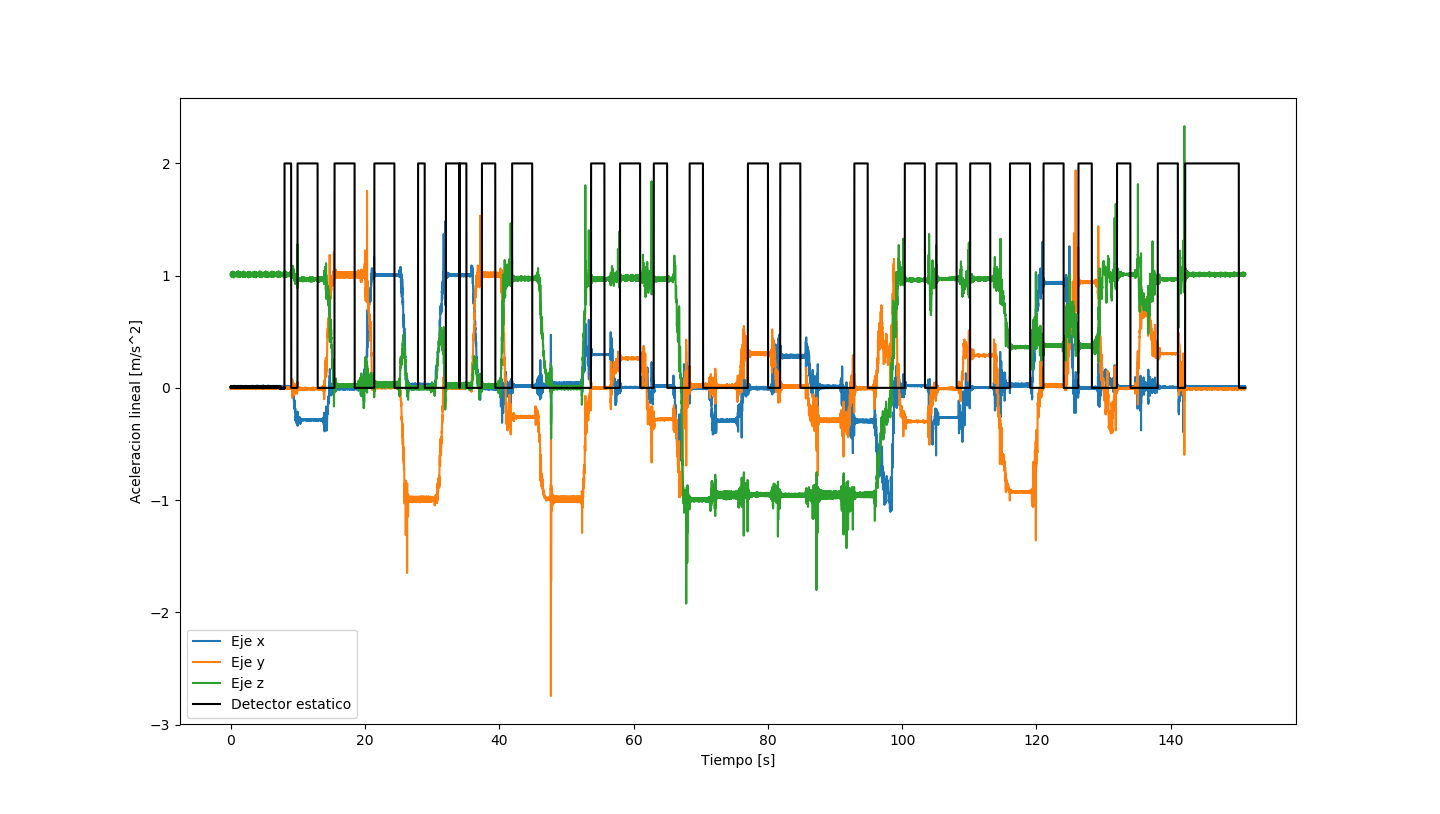
\includegraphics[width=\textwidth]{Img/IMUGyroAccelCal.png}
    \caption{Datos obtenidos del acelerómetro para utilizar en la calibración, incluyendo el detector de estáticos}
    \label{fig:imugyroaccelcal}
\end{figure}

En base a los intervalos estáticos, se procede al promediado de los intervalos, para luego utilizarlos en la función de coste de la Expresión (\ref{eq:generalaccelcostfunction}). Como para este caso particular los datos obtenidos del acelerómetro se encuentran normalizados, dicha Expresión puede simplificarse a la forma
\begin{equation}
    \mathscr{S}(\bm{\epsilon}_{a}) = \sum_{k=1}^M(1-||h(\bm{a}^s_k,\bm{\epsilon}_{a})||^2)^2
    \label{eq:mpu9250accelcostfunction}
\end{equation}
minimizándola mediante el algoritmo de Levenbeg-Marquandt, en base a los intervalos estáticos promediados. De la misma, se obtuvieron los siguientes parámetros
\begin{align}
        \bm{C}_a &=
    \begin{bmatrix}
        1 & -0.0369903 & -0.00491802 \\
        0 & 1 & -0.00370494 \\
        0 & 0 & 1
    \end{bmatrix}
    \\
        \bm{K}_a &=
    \begin{bmatrix}
        1.00014 & 0 & 0 \\
        0 & 0.999156 & 0 \\
        0 & 0 & 0.995609
    \end{bmatrix}
    \\
    \bm{b}_a &=
    \begin{bmatrix}
        -0.00401076 \\
        -0.00737427 \\
        -0.00671314
    \end{bmatrix}
\end{align}

\paragraph{Integración de la velocidad angular}
Como se desarrolló en la Sección \ref{sec:sensors}, la integración de la velocidad angular utilizando cuaterniones no es una tarea sencilla.
Esta función, en concreto, requiere de una integración de la velocidad angular en un tiempo discreto. Si bien existen diferentes métodos de integración numérica, es necesario que el mismo sea robusto y estable para mejorar la exactitud de la calibración. Por eso, el \textit{Runge-Kutta} $4^{th}$ \textit{order normalized method} (RK4n)\textbf{(Vojtesek, 2014)} es el elegido, aunque existen otros métodos que pueden utilizarse para este fin \textbf{(Andrle, 2013)}.

Si la ecuación diferencial que describe a la cinemática del cuaternión se define como
\begin{equation}
    \bm{f}(\bm{q},t) = \dot{\bm{q}} = \frac{1}{2}\bm{\Omega}(\bm{\omega}(t))\bm{q}
\end{equation}
donde $\bm{\Omega}(\bm{\omega}(t))$ es el operador que convierte la velocidad angular tridimensional considerada en la representación de la matriz simétrica oblicua real, esto es,
\begin{equation}
    \bm{\Omega}(\bm{w}) = 
    \begin{bmatrix}
        0 & -w_x & -w_y & -w_z \\
        w_x & 0 & w_z & -w_y \\
        w_y & -w_z & 0 & w_x \\
        w_z & w_y & -w_x & 0
    \end{bmatrix}
\end{equation}
El algoritmo de integración RK4n es
\begin{align}
    \bm{q}_{k} &= \bm{q}_{k-1} + \Delta t\frac{1}{6}(\bm{k}_1 +\bm{k}_2 + \bm{k}_3 + \bm{k}_4) \\
    \bm{k}_i &= \bm{f}(\bm{q}^{(i)},t_{k-1}+c_i\Delta t) \\
    \bm{q}^{(i)} &= \bm{q}_{k-1} &&\text{para} &&&i=1 \\
    \bm{q}^{(i)} &= \bm{q}_{k-1} + \Delta t\sum_{j=1}^{i-1}a_{ij}\bm{k}_j &&\text{para} &&&i>1
\end{align}
donde todos los coeficientes necesarios, $c_i$ y $a_{ij}$ son
\begin{align*}
    c_1 &= 0,\ c_2 = \frac{1}{2},\ c_3 = \frac{1}{2},\ c_4 = 1 \\
    &a_{21} = \frac{1}{2},\ a_{31} = 0,\ a_{41} = 0, \\
    &a_{32} = \frac{1}{2},\ a_{42} = 0,\ a_{43} = 1
\end{align*}

Finalmente, en cada paso, es necesario normalizar el cuaternión \textit{(k+1)-ésimo}, ya que puede exceder el valor unitario
\begin{equation}
    \bm{q}_{k+1} \rightarrow \frac{\bm{q}_{k+1}}{||\bm{q}_{k+1}||}
\end{equation}

\paragraph{Calibración del giróscopo}
\textbf{REVISAR LOS k y k+1!!!!!!!!}
Una vez calibrado el acelerómetro, se procede a la calibración del giróscopo utilizando el mismo dataset. Para ello, en primer lugar se obtiene el bias de giróscopo mediante el promedio de cada eje en el instante inicial $T_{init}$, obteniendo entonces
\begin{equation}
    \bm{b}_g =
    \begin{bmatrix}
         -0.00145159 \\
         0.00136245 \\
         0.0196623
    \end{bmatrix}
\end{equation}

A partir de estos valores, se plantea la resolución de la ecuación diferencial ordinaria mediante el algoritmo RK4n, y luego al cuaternión resultante se lo transforma en una matriz de rotación $\bm{\Lambda}(\bm{q}_{k+1})$ para ser aplicada al versor gravedad
\begin{equation}
    \bm{u}_{a,k-1} = \bm{g} =
    \begin{bmatrix}
        0 \\
        0 \\
        1
    \end{bmatrix}
\end{equation}
obteniendo entonces
\begin{equation}
    \bm{u}_{g,k} = \bm{\Lambda}(\bm{q}_{k+1})\bm{g}
\end{equation}

Finalmente, se reemplaza dicha magnitud dentro de la función de coste
\begin{equation}
    \mathscr{S}(\bm{\epsilon}_{g}) = \sum_{k=2}^M ||\bm{u}_{a,k} - \bm{u}_{g,k}||^2
\end{equation}
la cual se minimiza utilizando el algoritmo de Levenberg-Marquandt. Del mismo, se obtienen las matrices
\begin{align}
        \bm{C}_g &=
    \begin{bmatrix}
        1 & 0.0568771 & 0.0558162 \\
        0.253165 & 1 & -0.0749733 \\
        0.0284105 & -0.103141 & 1
    \end{bmatrix}
    \\
        \bm{K}_g &=
    \begin{bmatrix}
        1.19264 & 0 & 0 \\
        0 & 0.97173 & 0 \\
        0 & 0 & 1.0037
    \end{bmatrix}
\end{align}

\subsubsection{Calibración del magnetómetro}
asdasdsa

\subsection{Calibración de la cámara estéreo}
Siguiendo la metodología explicada en la Sección \ref{sec:sensors}, para la calibración de la cámara Minoru se utilizó un chessboard de 8x6, con cuadrículas de 10,8cm de lado, tal como la matriz presentada en el tutorial de calibración estéreo del paquete \texttt{camera\_calibration}\footnote{\url{http://wiki.ros.org/camera_calibration/Tutorials/StereoCalibration}}. Siendo que tanto en ROS como en OpenCV los extremos se buscan horizontalmente, es recomendable presentar el chessboard con la mayor cantidad de bordes de manera horizontal, tal como se observa en las calibraciones instantáneas de la Figura \ref{fig:minorurightleft}.

\begin{figure}[!ht]
    \centering
    \subfloat{{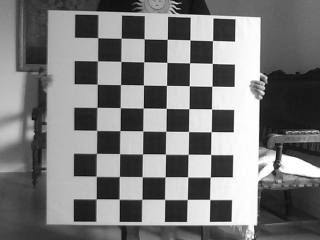
\includegraphics[width=0.45\textwidth]{Img/MinoruLeft.png}}}%
    \qquad
    \subfloat{{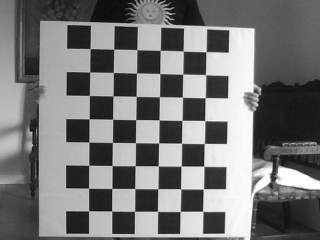
\includegraphics[width=0.45\textwidth]{Img/MinoruRight.png}}}%
    \caption{Imágenes izquierda y derecha de la calibración de la cámara Minoru}
    \label{fig:minorurightleft}
\end{figure}

Por razones de ancho de banda de USB 2.0, se configuraron las cámaras para trabajar en la resolución 320x240 a 30fps, consiguiendo entonces una imagen fluída, pero con una resolución limitada. A su vez, como la cámara utilizada no se encuentra sincronizada, es necesario realizar una aproximación entre ambas cámaras para tener mejores resultados en la calibración. Luego de un set de mediciones, se obtuvieron los datos de calibración de cada cámara, todos expuestos en dos archivos YAML, uno para la cámara derecha (Código \ref{lst:rightcamerayaml}) y otro para la cámara izquierda (Código \ref{lst:leftcamerayaml}).
\begin{lstlisting}[caption=YAML de la calibración de la cámara derecha mediante ROS, label=lst:rightcamerayaml]
image_width: 320
image_height: 240
camera_name: right_camera
camera_matrix:
  rows: 3
  cols: 3
  data: [ 435.736  ,    0.     ,  163.48678,
            0.     ,  436.74973,  117.12178,
            0.     ,    0.     ,    1.     ]
camera_model: plumb_bob
distortion_coefficients:
  rows: 1
  cols: 5
  data: [-0.139272, 0.228863, 0.000443, 0.002089, 0.000000]
rectification_matrix:
  rows: 3
  cols: 3
  data: [ 0.99997044, -0.00746816,  0.00182902,
          0.00746328,  0.99996861,  0.00266238,
         -0.00184884, -0.00264865,  0.99999478]
projection_matrix:
  rows: 3
  cols: 4
  data: [ 453.19158,    0.     ,  159.7411 ,  -27.55073,
            0.     ,  453.19158,  110.3157 ,    0.     ,
            0.     ,    0.     ,    1.     ,    0.     ]
\end{lstlisting}
\begin{lstlisting}[caption=YAML de la calibración de la cámara izquierda mediante ROS, label=lst:leftcamerayaml]
image_width: 320
image_height: 240
camera_name: left_camera
camera_matrix:
  rows: 3
  cols: 3
  data: [ 431.44958,    0.     ,  151.48809,
            0.     ,  432.60045,  103.73964,
            0.     ,    0.     ,    1.     ]
camera_model: plumb_bob
distortion_coefficients:
  rows: 1
  cols: 5
  data: [-0.088844, -0.120207, 0.001345, -0.002007, 0.000000]
rectification_matrix:
  rows: 3
  cols: 3
  data: [ 0.99989833, -0.0080206 , -0.01178974,
          0.00798926,  0.99996443, -0.0027027 ,
          0.011811  ,  0.00260823,  0.99992685]
projection_matrix:
  rows: 3
  cols: 4
  data: [ 453.19158,    0.     ,  159.7411 ,    0.     ,
            0.     ,  453.19158,  110.3157 ,    0.     ,
            0.     ,    0.     ,    1.     ,    0.     ]
\end{lstlisting}

\fi

\ifimagenes
\subsection{Experimentación con cámara estéreo}
Con el fin de utilizar datos reales, en principio se optó por usar la cámara estéreo Minoru 3D Webcam, la cual puede observarse en la Figura \ref{fig:minoru3dwebcam}. La misma cuenta con una interfaz USB 2.0 y una resolución de hasta 640x480, pudiendo además proporcionar hasta 30fps.
\begin{figure}
    \centering
    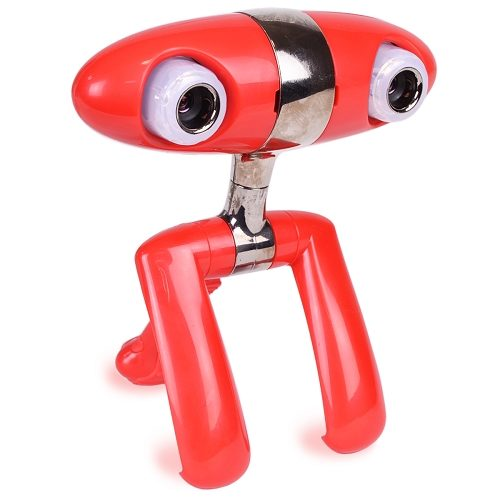
\includegraphics[width=0.2\textwidth]{Img/Minoru.jpeg}
    \caption{Cámara estéreo Minoru 3D Webcam}
    \label{fig:minoru3dwebcam}
\end{figure}

A pesar de estas especificaciones mencionadas anteriormente, no podría obtenerse una resolución de 640x480 a 30fps, debido a la limitación propia del USB 2.0. Por eso, se optó por trabajar con una resolución de 320x240 para poder mantener los fps.

\subsubsection{Calibración de la cámara}
Como la Minoru presenta la posibilidad de cambiar el enfoque de cada una de las cámaras monoculares, es necesario realizar una calibración de la misma cada vez que se realice un ajuste en dichos focos. Como en primera instancia se desconocía la calibración actual de dicha cámara, se optó por elegir un enfoque dado para luego calibrarla mediante el paquete de ROS \texttt{camera\_calibration}, presentado en la Sección \ref{sec:marcoteorico}. Para esto, se utilizó un chessboard de 8x6 con cuadrículas de 10,8cm de lado. Siendo que tanto en ROS como en OpenCV los extremos se buscan horizontalmente, es recomendable presentar el chessboard con la mayor cantidad de bordes de manera horizontal.

Luego de mover a la cámara en distintas orientaciones y consiguiendo por ende una buena cantidad de correlaciones entre las imágenes observadas en distintos patrones, se procede a la calibración de los datos obtenidos. Además de proveer con los archivos de calibración correspondientes, el paquete de ROS otorga las imágenes que fue tomando en cada caso (tanto izquierda como derecha) para cada una de las correspondencias que encontró en las imágenes. Por ejemplo, en la Figura \ref{fig:minorurightleft} puede observarse las vistas izquierda y derecha de cuando el algoritmo encontró una correspondencia entre ambas imágenes.

\begin{figure}[!ht]
    \centering
    \subfloat{{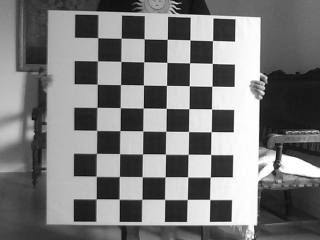
\includegraphics[width=0.45\textwidth]{Img/MinoruLeft.png}}}%
    \qquad
    \subfloat{{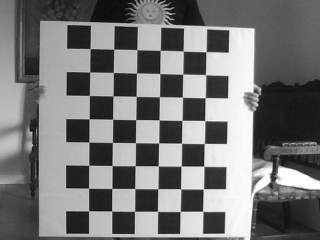
\includegraphics[width=0.45\textwidth]{Img/MinoruRight.png}}}%
    \caption{Imágenes izquierda y derecha de la calibración de la cámara Minoru}
    \label{fig:minorurightleft}
\end{figure}

\subsubsection{Nube de puntos obtenida}
Luego de la calibración, con el paquete de ROS \texttt{stereo\_image\_proc} se puede obtener el mapa de profundidades de la cámara. Además, como se mencionaba anteriormente, dicho paquete cuenta con una opción gráfica para poder configurar los parámetros de las correspondencias estéreo, facilitando la configuración del mismo. Finalmente, con dichos ajustes se obtiene la nube de puntos observada en la Figura \ref{fig:minorupointcloud}, donde en se encuentran las imágenes en crudo de las cámaras izquierda y derecha, la nube de disparidad calculada, y la nube de puntos final obtenida.

\begin{figure}[!ht]
    \centering
    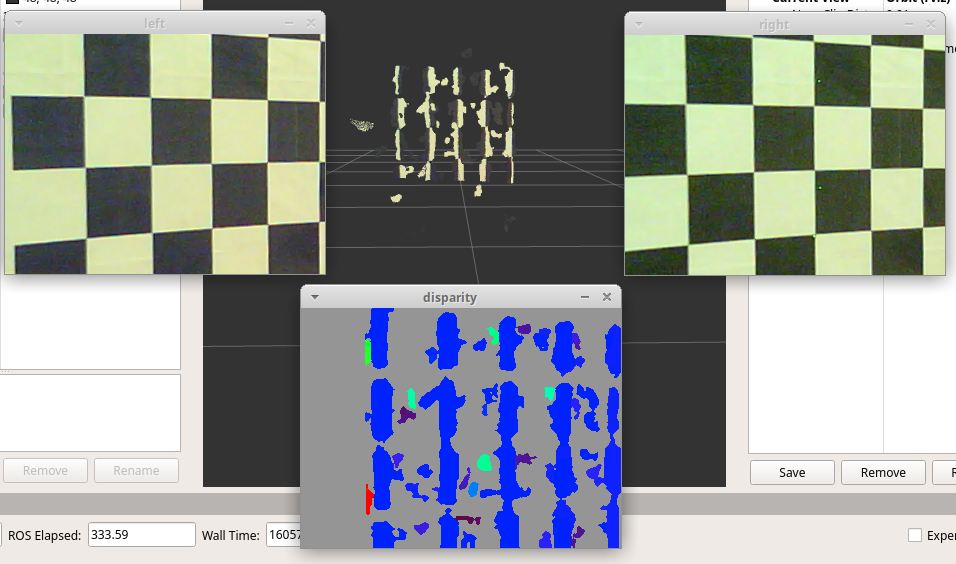
\includegraphics[width=\linewidth]{Img/MinoruPointCloud.png}
    \caption{Imágenes izquierda y derecha, disparidades y nube de puntos conseguida a partir de la cámara Minoru}
    \label{fig:minorupointcloud}
\end{figure}

Si bien la nube de puntos adquirida por el sensor presenta discontinuidades, con el procesamiento adecuado puede mitigarse este problema. Sin embargo, como las cámaras no están sincronizadas por hardware entre sí, y sumado a que al mover a la misma se aprecia una demora entre la imágen izquierda y derecha, la nube de puntos generada en movimiento no puede tomarse como válida, debido a no poder obtener una representación significativa del entorno con la misma.
% Si bien los resultados no sean ideales, a la hora de mover la cámara la misma presenta una demora, haciendo que lleguen retrasadas las imágenes izquierda y derecha y, por lo tanto, desincronizadas. Luego de llegar a este punto, se estudió el caso de la Minoru en particular y ambas cámaras no están sincronizadas por hardware, haciendo que el proceso sea complejo de realizarse en aplicaciones que requieran a un robot en movimiento.

\subsection{Registro de las nubes de puntos}
En base a datos de simulaciones en Gazebo, y tomando de base el Rosbot 3.0, se obtuvieron un set de grabaciones, en base a los datos arrojados por la Microsoft Kinect del mismo. Debido a que es una simulación, se tomó directamente la nube de profundidades dada por dicho 
\ifimagenespaper
modelo.
\else
modelo, aunque puede realizarse un proceso similar al descripto en el anexo del documento para obtener dicha nube de puntos de profundidad 3D.
\fi

\else
\subsection{Algoritmo SLAM propuesto}
Como los sensores exteroceptivos utilizados (LIDAR 2D y cámara estéreo) pueden generar mapas diferentes (aunque relacionados), para la implementación del algoritmo SLAM se propone el diagrama visible en la Figura \ref{fig:slamalgorithmblockdiagram}, donde se plantea un filtro de Kalman ''integrador'' para calcular la pose del vehículo, tomando en la etapa de predicción los datos de sensores propioceptivos, mientras que para la etapa de corrección utiliza cada estimación proporcionada por los sensores exteroceptivos (calculada en conjunto con sensores propioceptivos y el estado anterior estimado). Esta etapa de corrección se realiza cada vez que alguno de estos sensores exteroceptivos tiene una nueva estimación de la pose del vehículo.
\begin{figure}
    \centering
    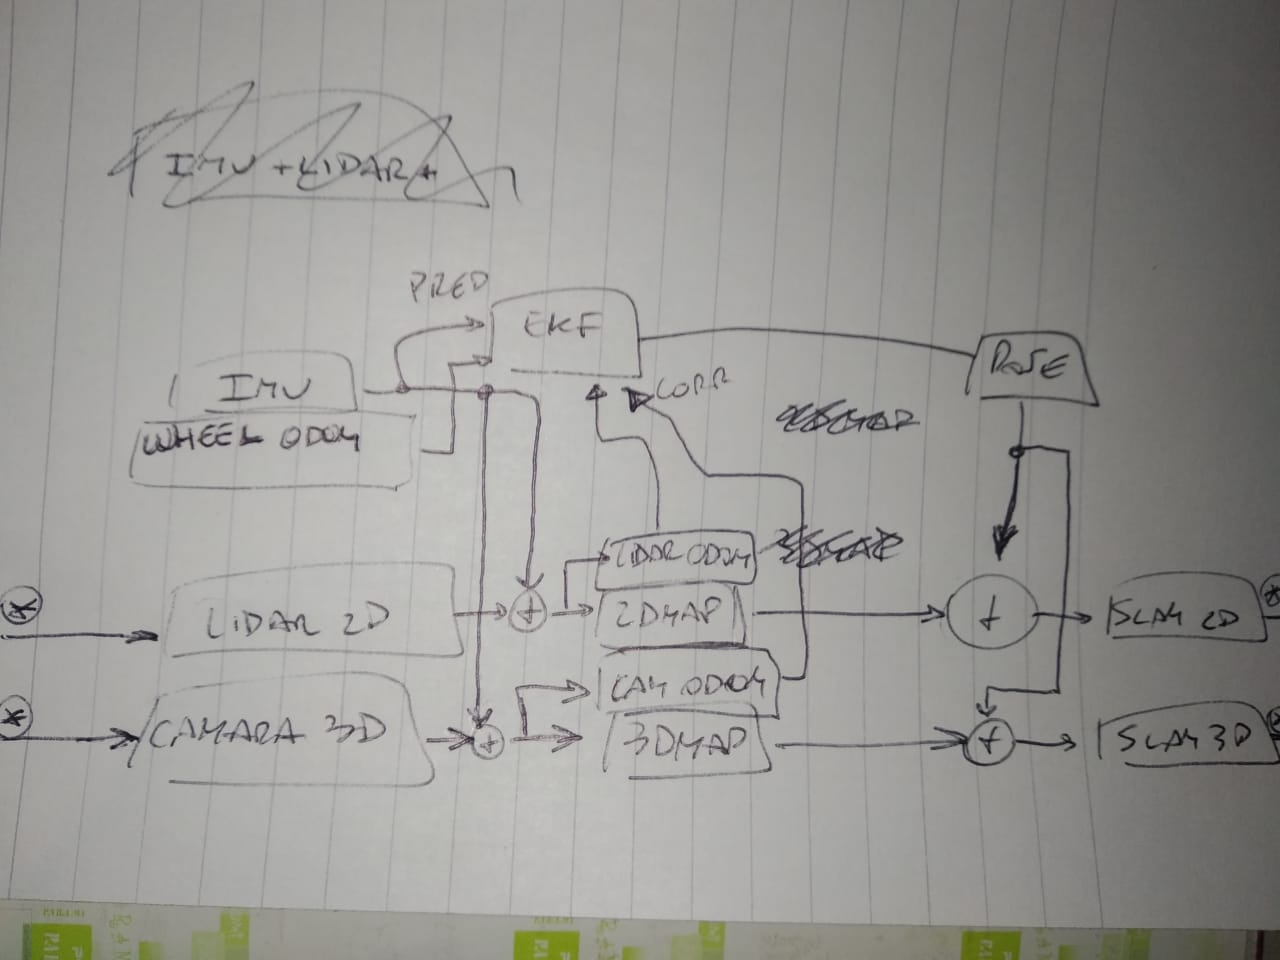
\includegraphics[width=\textwidth]{Img/SLAMAlgorithmBlockDiagram.jpeg}
    \caption{Diagrama en bloques del algoritmo SLAM propuesto}
    \label{fig:slamalgorithmblockdiagram}
\end{figure}

A continuación se presentarán los distintos algoritmos utilizados, al principio como cada uno por separado, para luego juntarlos en el EKF final.

\subsubsection{SLAM 2D}

\subsubsection{SLAM 3D}
\fi
Una vez con las nubes de puntos de profundidad provenientes de la cámara, el próximo paso refiere a la generación del mapa y la localización del robot en el entorno, utilizando el denominado \textit{registration pipeline} (presentado en la Sección \ref{sec:marcoteorico}). A continuación, se desarrollan los pasos realizados a estas nubes de puntos, los cuales pueden verse en la Figura \ref{fig:3dalgorithmblockdiagram}.

\begin{figure}
    \centering
    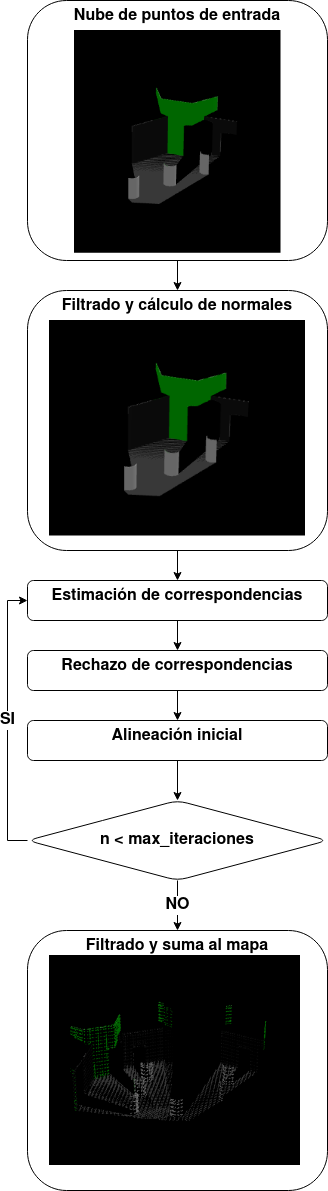
\includegraphics[scale=0.45]{Img/3DAlgorithmBlockDiagram.png}
    \caption{Diagrama en bloques del pipeline realizado para el registro de nube de puntos tridimensionales y su posterior actualización del mapa 3D}
    \label{fig:3dalgorithmblockdiagram}
\end{figure}

\subsubsection{Etapa de selección de datos}
Debido a que se utiliza una resolución de 640x480, hay una gran cantidad de puntos, haciendo que el costo computacional sea muy alto por cada corrida del algoritmo. Para ello, lo primero que se hace es un filtrado de dichos datos. Tal como se menciona en \cite{holz2015}, es importante conservar los bordes, por lo que el filtro bilateral es una buena opción. En PCL es implementado mediante \lstinline{pcl::FastBilateralFilter}.

Como vimos en la Sección \ref{sec:marcoteorico}, las normales de los puntos ayudan no solo en la etapa de rechazo de correspondencias, sino también puede ser útil en la etapa de filtrado, como es el caso de \textit{normal space sampling}. Debido a que los datos originales son del tipo \lstinline{pcl::PointXYZRGB}, es necesario calcular dichas normales. Un método rápido para hacer esto es mediante el uso de imágenes integrales \cite{holzer2012}. La ventaja de este método es que solo requiere una etapa de preprocesamiento lineal al tiempo que permite calcular los vectores medios y las normas dentro de un área rectangular de la imagen en tiempo constante. Por lo tanto, en primera instancia mediante la implementación de PCL \lstinline{pcl::IntegralImageNormalEstimation} se calculan las normales, para luego realizar el \textit{normal space sampling}.

Como el algoritmo de \textit{normal space sampling} requiere de una nube de puntos ordenada, luego de este proceso se procede a la remoción de los datos inválidos de las nubes de puntos, mediante la implementación de PCL \lstinline{pcl::removeNaNFromPointCloud}.

\subsubsection{Estimación de correspondencias}
Una vez obtenidos los puntos filtrados y con sus respectivas normales (dando lugar entonces a puntos del tipo \lstinline{pcl::PointXYZRGBNormal}), se procede al cálculo de las correspondencias entre las nubes de puntos.

\subsubsection{Rechazo de correspondencias}
Como se tienen tanto los datos de la posición como de la normal de cada punto, se emplean dos filtros de correspondencias
\begin{itemize}
    \item uno para filtrar la distancia mediante el uso de la mediana, dando lugar al \lstinline{pcl::registration::CorrespondenceRejectorMedianDistance}, y
    \item  un segundo filtro en base a las superficies normales, esto es, \lstinline{pcl::registration::CorrespondenceRejectorSurfaceNormal}, asignando un peso a las correspondencias en base al error que presentan las cámaras RGB-D \cite{nguyen2012}, el cual puede generalizarse al modelo presente en la Ecuación \ref{eq:weightcorrespondences}, considerando dos puntos $\bm{p}$ y $\bm{q}$
    \begin{align}
        w(\bm{p},\bm{q}) &= max(\sigma_z({\bm{p}_z}), \sigma_z(\bm{q}_z))
        \label{eq:weightcorrespondences} \\
        \text{con }\sigma_z(z) &= 0.0012+0.0019\cdot (z-0.4)^2
    \end{align}
\end{itemize}

En concreto, primero se realiza el filtro de mediana, y luego el filtro en base a la información de las normales.

\subsubsection{Alineación}
Finalmente, con las correspondencias restantes se procede al cálculo de la transformación que responde a las dos nubes de puntos. Para ello, se utiliza el principio de punto a plano, debido a su rápida convergencia y buena precisión comparado con el método de punto a punto. Por ello, utilizando la función de PCL \lstinline{pcl::registration::TransformationEstimationPointToPlaneWeighted} se llega a la transformación que describe en una primera instancia el movimiento realizado por el robot.

\subsubsection{Refinamiento y actualización}
Debido a los posibles mínimos locales encontrados en lugar del mínimo global, para poder encontrar la transformación adecuada, se itera en los pasos de estimación de correspondencias, el rechazo de las mismas y el cálculo de la transformada, realizando la transformación de la nube de puntos fuente (filtrada y con sus respectivas normales) en base al resultado anterior, para luego calcular dichos valores nuevamente.

Finalmente, con la tranformación calculada se aplica la misma a la nube de puntos fuente para, luego de un nuevo filtrado para reducir su tamaño, agregarla al mapa generado en base a las nubes de puntos previas. En PCL, haciendo simplemente una suma de dicha nube de puntos transformada con el mapa se consigue el objetivo.

\subsection{Resultados}
Debido a los problemas mencionados de la cámara Minoru para generar los mapas, sumado a que no se dispone del dato real de la trayectoria del robot para poder contrastarla con el algoritmo desarrollado, se cambió el enfoque del trabajo y se optó por obtener los datos en base a un entorno de simulación que, como se mencionó anteriormente, fue Gazebo el elegido. 

Dentro de los modelos que se encuentran disponibles, se tomó el modelo del robot terrestre  \textit{Rosbot 3.0}\footnote{https://github.com/husarion/rosbot\_description} para realizar las simulaciones, el cual cuenta con una Microsoft Kinect, además de contar con un LIDAR 2D, IMU y encoders. A su vez, el mismo fabricante proporciona mapas simulados para la realización de pruebas, y con el agregado de los mapas presentes en el robot \textit{Turtlebot3}\footnote{https://github.com/ROBOTIS-GIT/turtlebot3} se consiguen una suficiente cantidad de entornos para ensayar el algoritmo descripto. A continuación, se detallan los resultados en base a uno de los mapas y el \textit{Rosbot 3.0}.

Para el caso, se evaluó el mapa \textit{turtlebot3 world}, que se observa en la Figura \ref{fig:turtlebotworldoriginalmap}, además de observarse también el modelo simulado del Rosbot 3.0. A partir de dicha simulación, se movió al robot sin un patrón específico, tratando de que pueda mapearse todo el lugar, guardando los tópicos de interés en un contenedor de ROS (\textit{rosbag}) para luego poder procesar y evaluar la misma información con el fin de poder ajustar el algoritmo. En base a esto, se fue construyendo el mapa con cada una de las nubes de puntos entrantes, comparado a cada una con la nube de puntos anterior y sumando entonces la nueva nube transformada al mapa generado, mediante el \textit{registration pipeline} descrito anteriormente. En base a esto, se consiguieron los resultados que se observan en la Figura \ref{fig:turtlebotworldestimatedmap}, donde la traza roja representa a la trayectoria real del robot (dato proporcionado por la simulación), mientras que la trayectoria azul se trata de la trayectoria estimada por el algoritmo realizado.
\begin{figure}[!ht]
    \centering
    {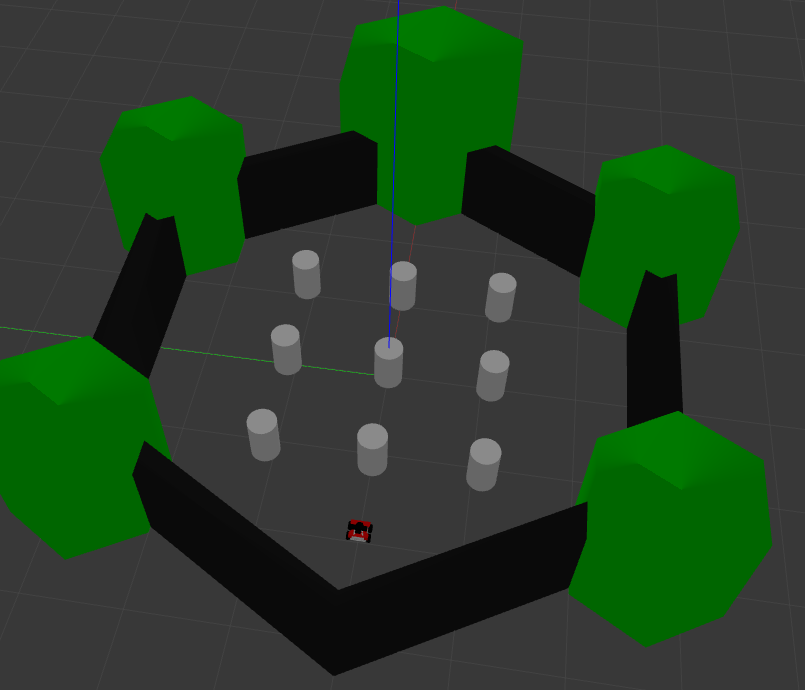
\includegraphics[width=\linewidth]{Img/TurtleBotWorldMap3D.png}}
    \caption{Entorno simulado \textit{turtlebot3 world}}
    \label{fig:turtlebotworldoriginalmap}
\end{figure}
\begin{figure}[!ht]
    \centering
    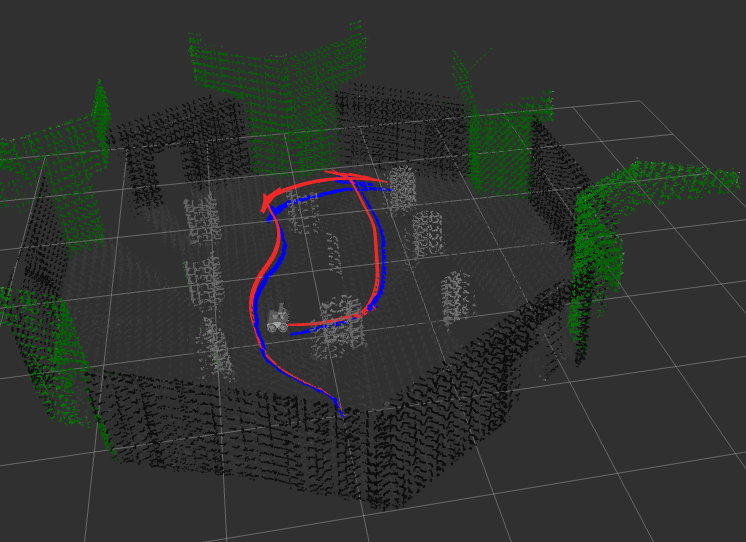
\includegraphics[width=\linewidth]{Img/TurtleBotWorldMap3DEstimated.png}%
    \caption{Mapa reconstruido en base a la cámara RGB-D del entorno simulado, junto a la trayectoria real y estimada por el algoritmo}
    \label{fig:turtlebotworldestimatedmap}
\end{figure}
Como el tiempo de procesamiento en una computadora de 4 núcleos (2.0 GHz) ronda el segundo, se redujo la tasa de ejecución del contenedor de ROS para poder procesar todas las nubes de puntos, ya que se consiguen datos cada medio segundo. 


Como se pretende realizar luego una fusión sensorial, combinando un LIDAR 2D y una IMU, una opción para que pueda llevarse al tiempo real es procesando cada cierto tiempo las nubes, ignorando entonces parte de ellas. Como el LIDAR 2D da información respecto a la pose del vehículo, se conseguirían entonces resultados aproximados, ya que para cada paso del algoritmo se partiría de la última transformación estimada, ya sea de la cámara, del LIDAR o de un algoritmo externo, como puede ser el filtro de Kalman.
        \section{Conclusiones}
\label{sec:5_concl}
\ifimagenes
En el trabajo presentado se logró en primera instancia realizar las comprobaciones prácticas en una cámara estereo para luego realizar un algoritmo de SLAM en base a los datos de una cámara RGB-D, con la capacidad de poder reconstruir un mapa símil al real, y obteniendo las poses relativas de cada iteración. Si bien es cierto que se realizaron las mediciones en base a simulaciones, el hecho de haber incorporado ROS permite que el código pueda adaptarse fácilmente no solo a un entorno real, sino también a cualquier robot, permitiendo entonces una gran flexibilidad a la hora de utilizarlo. 

Respecto a los tiempos de procesamiento del algoritmo, los mismos son suficientes para el movimiento de robots en velocidades moderadas, en cambio si se pretende utilizar al mismo a una gran velocidad es posible que no pueda obtener los resultados esperados, debido a que el algoritmo espera que la nube de puntos anterior no esté muy alejada de la nueva nube de puntos. 

\section{Trabajos futuros}
Este trabajo forma parte de un trabajo final de carrera en desarrollo, el cual pretende realizar un SLAM 2D y 3D aprovechando otros sensores para obtener el mapa final, en particular, una IMU y un LIDAR 2D. Por dicha razón es que el documente presentado es adecuado para dicha tarea ya que, por ejemplo, con los datos de un LIDAR 2D a la hora de correr el algoritmo en tiempo real, la pose anterior será la estimada por el LIDAR, haciendo que el punto de partida no esté muy lejos del resultado final, evitando así errores por no encontrar el mínimo global.

Como este proyecto se engloba dentro de un problema de SLAM con fusión sensorial entre la cámara, LIDAR 2D e IMU, se pretende que el algoritmo mejore considerablemente a la hora de realizar dicha fusión.
\else
En el trabajo presentado se logró, en primera instancia, el desarrollo de una plataforma versátil para aplicaciones robóticas en general. 

Luego, se realizaron distintas calibraciones de sensores de interés en las distintas áreas de la robótica, tal como la IMU y las cámaras.

A continuación, se realizaron las comprobaciones prácticas en una cámara estéreo para luego realizar un algoritmo de SLAM 3D en base a los datos de una cámara RGB-D, con la capacidad de poder reconstruir un mapa símil al real, y obteniendo las poses relativas de cada iteración. 

A su vez, con el uso de un LIDAR 2D ayudado por los datos de una IMU se consiguió resolver el problema de SLAM 2D, con tiempos considerables como para que el mismo pueda implementarse en tiempo real.

Si bien es cierto que se realizaron las mediciones en base a simulaciones, el hecho de haber incorporado ROS permite que el código pueda adaptarse fácilmente no solo a un entorno real, sino también a cualquier robot, permitiendo entonces una gran flexibilidad a la hora de utilizarlo. 

%Respecto a los tiempos de procesamiento del algoritmo, los mismos son suficientes para el movimiento de robots en velocidades moderadas, en cambio si se pretende utilizar al mismo a una gran velocidad es posible que no pueda obtener los resultados esperados, debido a que el algoritmo espera que la nube de puntos anterior no esté muy alejada de la nueva nube de puntos. 

\fi
        \bibliographystyle{unsrt}
        \bibliography{thebibliography}
    \else
        \centering
        \begin{figure}[t]
        	\centering
        	
\includegraphics[scale=0.15]{utn.jpg}
            \vspace{0.5cm}
        \end{figure}%
    \fi
\fi

\ifimagenes
	{\LARGE Procesamiento digital de imágenes\par}
    {\LARGE 2020\par}
	\vspace{1cm}
	{\huge\bfseries SLAM 3D basado en cámara RGB-D y PCL\par}
\else
	{\LARGE Proyecto Final\par}
    {\LARGE 2020\par}
	\vspace{1cm}
	{\huge\bfseries Robots con detección de entorno\par}
	\vspace{1cm}
    {\LARGE Trabajo final de carrera\par}
\fi
    \vspace{1cm}
	{\Large\itshape Domínguez, Francisco\par}
	\vfill
\end{titlepage}

\tableofcontents

\newpage
\listoffigures
\ifimagenes
\else
    \newpage
    \listoftables
    \newpage
    \section*{Objeto del Documento}
\label{sec:0_objeto}
El objeto del presente es hacer un análisis exhaustivo del estado de las plataformas de Hardware presentes en el mercado actual, de manera de diseñar a partir de dicho análisis una plataforma versátil para el usuario que permita extender el rango de aplicaciones de las plataformas ya existentes, permitiendo así, por ejemplo, el montaje de sensores adicionales a la placa. En base a dicho diseño, se implementa una solución al problema de la localización y mapeo simultáneos (SLAM).
\fi

\newpage
\section*{Abstract}
\label{sec:1_abstract}

En los últimos años, los robots han recibido una mayor atención de la comunidad de investigación, en especial debido a la aparición de los vehículos aéreos no tripulados.

El presente trabajo describe el desarrollo de una plataforma de control de robots. Dicha plataforma cuenta con la posibilidad de expandir sus funcionalidades gracias al estándar de hardware PC/104 presente en la industria, logrando así poder desarrollar a partir de la misma tanto vehículos aéreos no tripulados (UAV) como robots terrestres, entre otros. En base a la misma, se desarrollará un robot capaz de estimar tanto su posición como el contorno del mapa en el cual se encuentra.


\newpage
\section{Introducción}
\label{sec:2_marcoteorico}
Si bien el uso de robots tiene sus orígenes principalmente en fábricas para el ensamblaje de automóviles, en los últimos años la electrónica moderna ha permitido introducirlos en otras áreas, ya sea desde electrodomésticos y juguetes de la vida cotidiana, hasta viajes espaciales con el fin de explorar planetas desconocidos. Esta expansión es debido a que los mismos permiten reducir la interacción humana no solo en tareas que presentan un riesgo a la integridad de la persona, sino también en aquellas que tienen cierto grado de repetitividad.

Yendo a un caso más concreto, en el último tiempo muchas personas han adquirido los llamados robots aspiradoras, como el que se observa en la Figura \ref{fig:vaccumrobot}.a, los cuales consiguen limpiar la superficie de las casas en un tiempo medianamente razonable, aunque este tiempo no suele ser una preocupación ya que al ser el mismo completamente autónomo, uno puede seguir con sus actividades cotidianas. 

No obstante, si se analiza el recorrido que realizan la mayoría de estos robots, se puede apreciar que el mismo suele ser completamente aleatorio, y por ende se tendería a creer que no podrá pasar por toda la superficie y limpiarla completamente. La realidad es que, como están mucho tiempo circulando, logran pasar por todos los rincones de la superficie, pero esto genera que circulen más veces por unos lugares que por otros, tal como se observa en la Figura \ref{fig:vaccumrobot}.b, haciendo ineficiente el trabajo.

\begin{figure}[!ht]
    \centering
    \subfloat[Robot aspiradora comercial]{{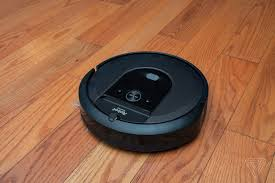
\includegraphics[width=0.47\textwidth]{Img/Roomba}}}%
    \qquad
    \subfloat[Ejemplo del recorrido de un robot aspiradora comercial]{{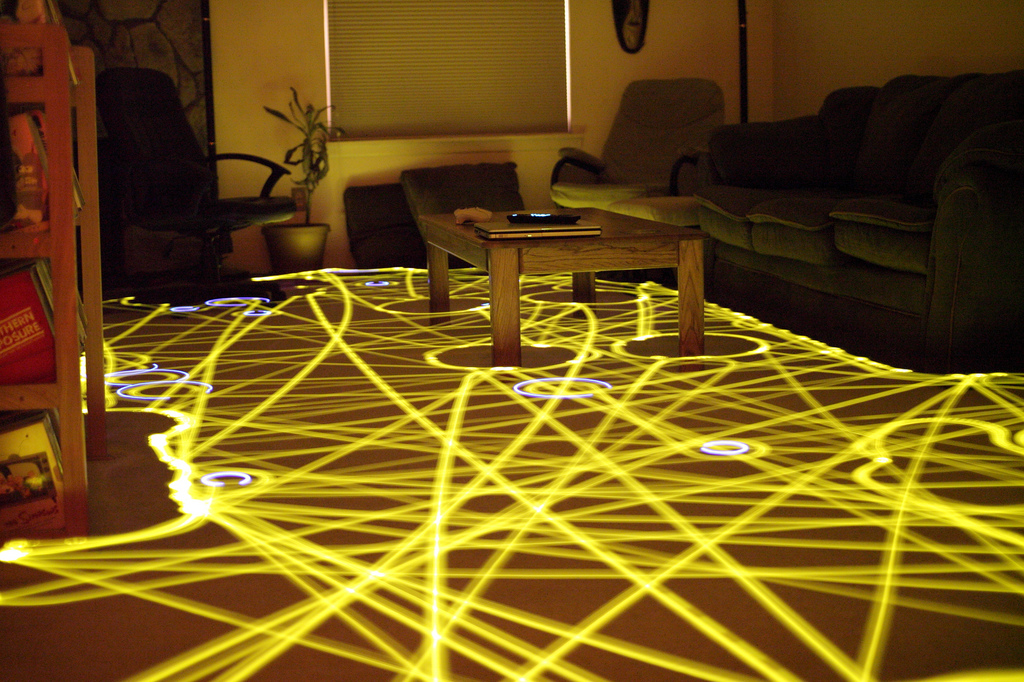
\includegraphics[width=0.47\textwidth]{Img/VaccumRobot.png}}}%
    \caption{El robot aspiradora}
    \label{fig:vaccumrobot}
\end{figure}

\ifimagenes
Si lo que se pretende es optimizar el recorrido del robot, la
\else
A pesar de que se busque reducir la interacción humana bajo estas circunstancias, no todos los robots hoy en día son autónomos, principalmente debido a la falta de robustez del algoritmo de control involucrado en el proceso. Tomando por caso el ejemplo anterior, si bien el robot aspiradora es autónomo, su eficiencia respecto a la forma óptima de realizar la tarea no es una garantía en todos los casos.

Es útil distinguir entre robots que están inmóviles, como un brazo robótico en una fábrica, y robots que son móviles, como un auto sin conductor. En este trabajo se hará hincapié en los robots móviles. Usamos este término para describir un robot impulsado por sus propios medios que puede moverse cinemáticamente entre ubicaciones en su entorno. A su vez, cuando se habla de la posición y orientación combinadas del robot, esto se define como su \textit{pose}.

Los robots móviles pueden referirse a robots que se mueven sobre el suelo, bajo el agua, a través del aire y en entornos de microgravedad, tales como los que pueden observarse en la Figura \ref{fig:mobilerobots}. Si bien este trabajo busca aplicar en parte a cualquiera de estos entornos, el enfoque del mismo se refiere principalmente a los robots móviles que permanecen en contacto con el suelo. Cada uno de ellos presentan su propia terminología para definirlos y diferenciarlos del resto, por ejemplo, el término vehículos terrestres no tripulados o UGV (del inglés \textit{unmanned ground vehicles}) a menudo se usa más específicamente para describir robots móviles terrestres, mientras que el término vehículos aéreos no tripulados o UAV (del inglés \textit{unmanned aerieal vehicles}) refieren principalmente a los drones.

Los robots móviles se mueven a través de entornos grandes y potencialmente dinámicos, lo que hace que la percepción sea mucho más difícil que los robots industriales con entornos de trabajo limitados y parámetros operativos rígidos. Por lo tanto, los robots móviles requieren sensores adicionales, una mejor percepción y mayores grados de autonomía para operar en entornos del mundo real que cambian con frecuencia.


\begin{figure}%
    \centering
    \subfloat[Wheeled robot]{{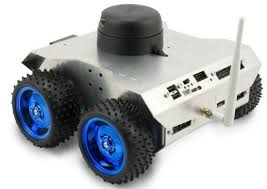
\includegraphics[width=0.25\linewidth]{Img/WheeledRobot.jpeg}}}%
    \qquad
    \subfloat[Legged robot]{{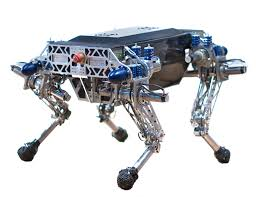
\includegraphics[width=0.25\linewidth]{Img/LeggedRobot.jpeg}}}%
    \qquad
    \subfloat[Tracked robot]{{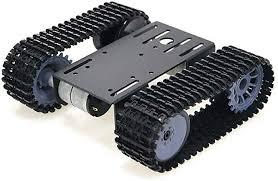
\includegraphics[width=0.25\linewidth]{Img/TrackedRobot.jpeg}}}%
    \qquad
    \subfloat[Drone]{{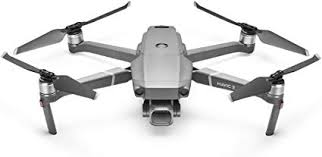
\includegraphics[width=0.3\linewidth]{Img/Drone.jpeg}}}%
    \qquad
    \subfloat[Water-based robot]{{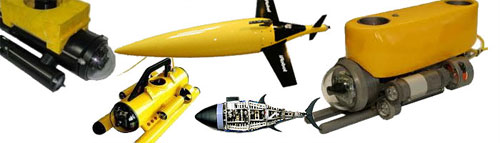
\includegraphics[width=0.5\linewidth]{Img/WaterBasedRobot.jpg}}}%
    \caption{Tipos de robot móviles}
    \label{fig:mobilerobots}
\end{figure}

Dentro de lo que respecta a robótica móvil, uno de sus desafíos actuales es lograr la completa autonomía del vehículo. Una gran parte de las empresas de la industria automotriz han dedicado mucho tiempo y dinero para lograr el objetivo. La investigación ha avanzado hasta el punto de que en la actualidad hay autos semi-autónomos disponibles en el mercado, y se cree ampliamente que en el futuro cercano casi todos los vehículos serán completamente autónomos. Para lograr esto, obviamente hay una necesidad de sensores y funciones avanzadas. Uno de los principales problemas es el hecho de que el vehículo debe ser consciente de su posición actual dentro de un entorno desconocido. Este proceso de determinar no solo su posición, sino también el mapa que lo rodea se conoce como la \textit{localización y mapeo simultáneos}, comúnmente abreviado como \textit{SLAM} (del inglés, \textit{simultaneous localization and mapping}).

El SLAM es un problema difícil de solucionar, así como lo fue para los humanos en el pasado. Tiempo atrás, los marineros usaban los llamados registros de fichas para estimar su velocidad y extrapolaban esta velocidad con el tiempo para calcular su pose. Este proceso de navegación por estima (en inglés, \textit{dead reckoning}) conduce inevitablemente a errores graves de posicionamiento con el tiempo y, por lo tanto, siempre se ha respaldado mediante el uso de puntos de referencia (o \textit{landmarks}) para la navegación. Quedándonos en este caso particular, con el uso de las estrellas los marineros lograban saber donde estaba el Norte, permitiendo corregir su dirección. Sin embargo, no siempre se podía observar este patrón por días debido al cielo nublado, entonces tenían que confiar solamente en su navegación por estima, haciendo que la incertidumbre crezca día tras día. Para el caso de los robots, cuando el mismo recorre un mapa completamente desconocido, acumulará error debido a las predicciones que debe tomar respecto a su pose y entorno en el que está, hasta el momento en que entra a un área con puntos de referencia conocidos, pudiendo así corregir su estimación de posición.

Volviendo al ejemplo del robot de limpieza, si el mismo conociera el mapa en el que se encuentra, podría entonces trazar la ruta mas óptima para realizar la limpieza del lugar. Como no todos los ambientes son iguales y cada uno tiene, por ejemplo, muebles ubicados en distintos lugares, dicho robot podría hacer primero un reconocimiento del lugar previo a la limpieza para tener una noción de todo el espacio, o bien obtener el mapa y la ubicación en la que se encuentra en base al movimiento que realiza, pasando por los lugares que le faltaron aspirar. Para cualquiera de las dos opciones, por lo tanto, necesitará tanto tomar los datos del lugar como controlar al vehículo para que vaya circulando por el ambiente.

La
\fi
estimación de la pose, entonces, es una parte no separable de aplicaciones como el control del vehículo y el mapeo. Varios sensores se utilizan comúnmente para estimar la pose de un robot. Las unidades de medición inercial (IMU), la cámara, la odometría de las ruedas\footnote{Se mide la rotación de las ruedas para estimar cambios de la posición del vehículo a lo largo del tiempo} para el caso de ciertos robots móviles y el LiDAR se encuentran entre los sensores más populares para la localización en interiores \cite{delrosario2016}, mientras que para exteriores suele sumarse el GPS a estos sensores, corrigiendo al mismo mediante acción de la IMU \cite{caron2006}.


\ifimagenes
\else
En la localización al aire libre, la señal del sistema de posicionamiento global (GPS) suele estar disponible y, dado que la posición se puede obtener con precisión mediante GPS, es la opción común para la fusión con los datos obtenidos de la IMU \cite{engel2014}. Sin embargo, en un entorno denegado por GPS, como dentro de un edificio, se deben usar otros sensores para corregir las estimaciones de la IMU. Un enfoque común para abordar este problema son la fusión IMU-cámara \cite{mirzaei2008}, \cite{hesch2009}, \cite{chambers2014}, \cite{hesch2013}, así como también el uso de LiDAR \cite{lee2016}.

Un algoritmo SLAM robusto es esencial para que cualquier robot móvil navegue de manera segura a través de un entorno no estructurado. El algoritmo SLAM con frecuencia define un marco de coordenadas global para que el robot opere; uno que generalmente es utilizado por todas las funcionalidades de alto nivel, como navegación, planificación de rutas, exploración, identificación de objetos, seguimiento de objetos y manipulación de los mismos. Estas dependencias hacen que el algoritmo SLAM sea una parte central de cualquier arquitectura de robot móvil, y las fallas irrecuperables son altamente indeseables. Es probable que cualquier robot desorientado por una falla de SLAM no pueda realizar su tarea, o peor, puede poner en peligro a los humanos, a sí mismo o al medio ambiente.

%Si bien se han demostrado varios algoritmos SLAM en laboratorios, es más difícil producir soluciones robustas en entornos no estructurados del mundo real. El deslizamiento de las ruedas, por ejemplo, puede producir mediciones de odometría ruidosas, mientras que los sensores del sistema de posicionamiento global (GPS) a menudo producen una localización global con saltos muy pronunciados para la misma posición. El SLAM robusto del mundo real se vuelve aún más difícil cuando estos errores de detección aleatorios y sistemáticos ocurren en entornos que tienen geometrías redundantes u objetos en movimiento. Por ejemplo, en el caso de los LIDAR bidimensionales, los algoritmos empleados con los mismos suelen presuponer que el robot se encuentra terrestre se encuentra sobre una superficie plana, tal como puede ser el cuarto de un hogar. Si la superficie presenta irregularidades muy marcadas, la tarea de mapeo en dos dimensiones del mismo aumentaría su complejidad, ya que no podría encontrar las relaciones entre los datos anteriores con los actuales (no coincidirían) por si solo, y dependería de sensores adicionales, como una IMU.

%Para poder realizar las tareas en tiempo real, es necesario contar con una capacidad de cómputo suficiente para no sólo adquirir todos los datos de los sensores, sino también procesarlos para conseguir el mapa junto a la pose en cada momento. En el presente trabajo, se desarrolla una plataforma de Hardware capaz de realizar dicha actividad, a su vez de describir dos algoritmos de SLAM, uno basado en la combinación de un LIDAR 2D junto a una IMU, y el otro basado en una cámara RGB-D, obteniendo entonces un SLAM tridimensional.
\fi



En particular, para el caso de la localización y mapeo tridimensional (SLAM 3D), los LIDAR 3D han adquirido bastante popularidad en el último tiempo con la llegada de los vehículos autónomos, aunque son muy costosos. Si se pretende entonces una opción más económica, las cámaras estéreo y RGB-D (\textit{D: Depth - profundidad}) son de las más utilizadas para esto, a su vez de poder obtener datos de color de las mismas. Los sensores RGB-D como la \textit{Microsoft Kinect} proporcionan directamente mapas de profundidad densos e imágenes en color. En general, los enfoques SLAM que operan en imágenes RGB-D son estructuralmente diferentes de los sistemas estéreo, ya que la entrada es RGB-D de profundidad en lugar de dos imágenes de color. A pesar de esto, pueden obtenerse nubes de puntos de profundidad a partir de ambos sensores con el procesamiento
\ifimagenes
\ifimagenespaper
adecuado, como los presentados por la librería OpenCV \cite{kaehler2017}.
\else
adecuado, lo cual se desarrolla en el apéndice.
\fi
\else
adecuado, como los presentados por la librería OpenCV \cite{kaehler2017}.
\fi

Una vez obtenidas las nubes de puntos de profundidad, una de las formas de calcular la posición y orientación del robot (conocido como la \textit{pose} del robot) a lo largo del tiempo es mediante la comparación entre dos nubes de puntos contiguas (una con los datos recientes y otra con los datos de la nube de puntos anterior), buscando en definitiva la transformación necesaria para que la nube de puntos actual pueda alinearse (o sea, que coincida lo mejor posible) con la nube de puntos anterior. Este proceso se lo conoce como el \textit{registro de la nube de puntos}, y suele llevar una serie de pasos, lo cual se desarrollará más adelante. Para poder facilitar el uso de nubes de puntos, existen librerías específicas para trabajar con dicha información, siendo algunas de ellas la \textit{Point Cloud Library} y \textit{Open3D}, las cuales implementan no sólo distintos algoritmos, sino también estructuras para facilitar el manejo de las nubes de puntos.

Si bien hay muchos robots móviles hoy en día en el mercado, gran parte de ellos son costosos, y sobre todo los que se encuentran equipados para realizar SLAM 3D. Para poder evaluar los algoritmos necesarios sin tener que ponerse en gasto, existen entornos de simulación pensados, entre otras cosas, para robots, consiguiendo resultados comparables con los reales. Unos de los más conocidos en el ámbito son \textit{V-REP} y \textit{Gazebo}, siendo este último el elegido para realizar el trabajo.

\subsection{Contribuciones}
En el presente trabajo, 
\ifimagenes
se desarrolla un algoritmo de registro de nube de puntos en base a los datos obtenidos de una cámara RGB-D en movimiento dentro de un ambiente estático, bajo el entorno de simulación Gazebo. En base a la transformación obtenida en cada iteración, se aplica la misma a la nube de puntos entrante, para luego sumarla al mapa 3D generado.

Como el trabajo presentado forma parte de una tesis de grado en desarrollo sobre SLAM 2D y 3D, se pretende que el mismo pueda fusionarse con los datos provenientes de otros sensores, en particular la IMU y el LIDAR 2D, para obtener una mejor estimación de la posición y, por consiguiente, obtener un mapa más exacto.

\else
se presenta una plataforma de Hardware capaz de realizar las tareas de SLAM que incluyen una gran cantidad de sensores, a su vez de contar la misma con un factor de forma de Hardware para que la misma pueda expandir sus funcionalidades en base a lo que requiera el usuario.

Luego, e describen dos algoritmos de SLAM, uno basado en la combinación de un LIDAR 2D junto a una IMU, y el otro basado en una cámara RGB-D, obteniendo entonces un SLAM tridimensional, ambos considerando un entorno estático. Debido a la falta de sensores capaces de brindar la información reuqerida, se realizaron las pruebas del mismo bajo el entorno de simulación Gazebo, con el fin de poder luego llevarlas a un escenario real cuando se tenga el robot completo.
\fi

A su vez, se provee de un código compatible con \textit{ROS}, un framework pensado para utilizar en robótica, permitiendo portabilidad y versatilidad a la hora de proporcionar los datos de los sensores, ya que el mismo utiliza un sistema de mensajes que permite vincular a dos procesos sin importar el método de adquisición o procesamiento de los datos, mientras los mismos respeten el tipo de mensaje en sí.

\subsection{Estructura del documento}
El presente documento se compone de las siguientes secciones
\ifimagenespaper
\else
y apéndices
\fi
\begin{itemize}
    \item \textbf{Introducción}: esta sección hace una breve introducción al SLAM, presentando los distintos sensores utilizados normalmente, a su vez de dar una primera aproximación al registro de nubes de puntos con los sensores RGB-D para realizar dicha tarea. A su vez, se mencionan las contribuciones realizadas.
    \ifimagenespaper
    \item \textbf{Marco teórico}:
    \else
    \item \textbf{Herramientas para el desarrollo de robots}: En esta sección se da una introducción al framework \textit{ROS}, en particular a su estructura y su modo de vinculación entre los distintos paquetes. Finalmente, se da una breve descripción de Gazebo.
        \ifimagenes
    \item \textbf{Marco teórico}:
        \else
    \item \textbf{Geometría tridimensional y marcos de referencia}: en esta sección se desarrollan los conceptos de la geometría tridimensional necesarias para abordar los temas del trabajo realizado, a su vez de mencionar distintos marcos de referencia usualmente utilizados.
    \item \textbf{Análisis de regresión}: en esta sección se desarrolla el denominado análisis de regresión, abarcando tanto la regresión lineal como la no lineal.
    \item \textbf{Estimación de estado}: siguiendo con el análisis de regresión, en esta sección se desarrollan distintos algoritmos de estimación de estado, siendo uno de los mas conocidos el filtro de Kalman.
    \item \textbf{Sensores}: en esta sección se mencionan distintos sensores utilizados comúnmente en lo que refiere al SLAM, a su vez de presentar distintos métodos de calibración de algunos de ellos y características importantes.
    \item \textbf{Simultaneous Localization And Mapping}: en esta sección se profundiza en lo que refiere al SLAM, mencionando no sólo distintos algoritmos que existen, sino también mencionando características importantes de la técnica en si.
    \item \textbf{Reconstrucción del entorno}:
        \fi
    \fi 
    en esta sección se describe tanto el flujo de trabajo del registro de nubes de puntos asi como también los distintos algoritmos utilizados comúnmente a la hora de realizarlo, asociando a los mismos con su implementación en la librería PCL. A su vez, se comenta como conseguir las nubes de puntos en base a los sensores utilizados comúnmente en este tipo de
    \ifimagenes
    aplicaciones, además de una calibración de los mismos.
    \item \textbf{Experimentos}: En base a la sección anterior, en esta se describe el flujo del algoritmo realizado, además de presentar los resultados obtenidos en base a la simulación realizada
    \else
    aplicaciones.
    \item \textbf{Plataformas disponibles}: en base a los sensores y datos necesarios, en esta sección se realiza un relevamiento de las distintas plataformas disponibles en el mercado, comparando cada una de ellas.
    \item \textbf{Resolución}: en esta sección se mencionan los métodos utilizados para lograr el objetivo del trabajo, basándose en las secciones anteriores. A su vez, se muestran los resultados obtenidos.
    \fi
    \item \textbf{Conclusiones}: En esta sección se desarrolla la finalidad conseguida del trabajo, evaluando distintos puntos de interés.
    \ifimagenes
    \item \textbf{Trabajos futuros}: en esta sección se mencionan distintos aspectos para lo que sigue luego de este trabajo.
    \else
    \item \textbf{Apéndices}: en esta sección se incluye información útil, como el esquemático de la placa realizada.
        \ifimagenespaper
        \else
    \item \textbf{Anexo}: Finalmente, se incluye un anexo con información útil a la hora de querer llevar a cabo una implementación con sensores físicos, utilizando los datos proporcionados por los mismos.
        \fi
    \fi
\end{itemize}

\subsection{Resumen}
En esta Sección se dio una introducción respecto a los temas que va a abordar el trabajo realizado, a su vez de mencionar las contribuciones por el mismo y, finalmente, mencionar las distintas secciones que se incluyen.

\newpage
\section{ROS}

Robot Operating System (ROS) es un \textit{framework} open source pensado para escribir software orientado a robots. Este software está estructurado como un gran número de pequeños programas que se pasan rápidamente los mensajes entre sí. Este paradigma fue elegido para fomentar la reutilización de software de robótica fuera del robot y del entorno en particular que impulsó su creación. Es por ello que cuenta con librerías, herramientas y convenciones que buscan facilitar la tarea de realizar comportamientos robustos y complejos de casi cualquier tipo de robot existente.

\ifimagenes
\else
    \newpage
    \section{Geometría tridimensional y marcos de referencia}
En la presente sección se presentará la geometría tridimensional y específicamente el concepto de rotación y traslación, junto con algunas de sus representaciones. Si se quiere profundizar en este tema, puede referirse a Barfoot \cite{barfoot2020}.%\textbf{(Barfoot, 2016)}.

Los robots móviles generalmente son libres de trasladarse y rotar. Matemáticamente, tienen seis grados de libertad: tres en traslación y tres en rotación. Esta configuración geométrica de seis grados de libertad se conoce como la \textit{pose} (posición y orientación) del robot. Algunos robots pueden tener múltiples cuerpos conectados entre sí; en este caso cada cuerpo tiene su propia pose. Consideraremos solo el caso de un solo cuerpo en el presente trabajo.

\subsection{Rotaciones}
El vector, $\undervec{r}$, es un objeto geométrico que tiene magnitud y dirección. Este vector puede ser expresado en un \textit{marco de referencia}, $\undervec{\bm{\mathcal{F}}}_a$, como
\begin{align}
    \undervec{r} &= r_1\undervec{a}_1+ r_2\undervec{a}_2 + r_3\undervec{a}_3 \\
    &= 
    \begin{bmatrix}
    r_1 & r_2 & r_3
    \end{bmatrix}
    \begin{bmatrix}
    \undervec{a}_1 \\ 
    \undervec{a}_2 \\
    \undervec{a}_3
    \end{bmatrix}
    \\
    &= \bm{r}_a^T\undervec{\bm{\mathcal{F}}}_a
\end{align}
donde $\undervec{\bm{\mathcal{F}}}_a$ contiene a los \textit{vectores base}, formando así el marco de referencia $a$, mientras que $\bm{r}_a$ es una matriz columna que contiene los \textit{componentes} o \textit{coordenadas} de $\undervec{r}$ en el marco de referencia $\undervec{\bm{\mathcal{F}}}_a$. De forma análoga, el vector $\undervec{r}$ puede ser escrito como
\begin{equation}
    \undervec{r} = \undervec{\bm{\mathcal{F}}}_a^T \bm{r}_a
\end{equation}

\subsubsection{Matriz de rotación}
Si se quisiera expresar al vector $\undervec{r}$ para dos marcos de coordenadas distintos, como puede verse en la Figura \ref{fig:rotatedcoordinateframes}, para cada uno de los marcos dicho vector será representado como
\begin{align}
    \undervec{\bm{\mathcal{F}}}_a &\rightarrow \bm{r}_a \\
    \undervec{\bm{\mathcal{F}}}_b &\rightarrow \bm{r}_b
\end{align}
% \begin{figure}
%     \centering
%     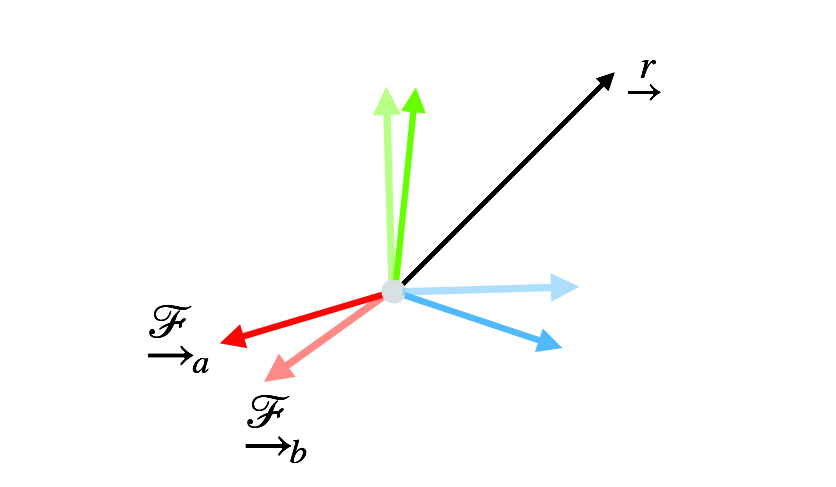
\includegraphics[width=\textwidth]{Img/RotatedCoordinateFrames.png}
%     \caption{Dos marcos de coordenadas con un vector en el espacio fijo}
%     \label{fig:rotatedcoordinateframes_old}
% \end{figure}

\begin{figure}
    \centering
    \tdplotsetmaincoords{50}{140}
\begin{tikzpicture}[scale=4,baseline,tdplot_main_coords]
    \coordinate (O) at (0,0,0);
    
    \draw[thick,->] (0,0,0) -- (1,0,0) node[anchor=north west]{$\undervec{\bm{\mathcal{F}}}_a$};
    \draw[thick,->] (0,0,0) -- (0,1,0);
    \draw[thick,->] (0,0,0) -- (0,0,1);
    
    \draw[thick,->,blue] (0,0,0) -- (0,1,1) node[anchor=north west]{$\undervec{\bm{r}}$};
    
    \pgfmathsetmacro{\ax}{2}
    \pgfmathsetmacro{\ay}{2}
    \pgfmathsetmacro{\az}{1}
    
    \tdplotsetrotatedcoords{20}{20}{0}
    
    \draw[->,tdplot_rotated_coords,red] (0,0,0) -- (.7,0,0) node[anchor=north west]{$\undervec{\bm{\mathcal{F}}}_b$};
    \draw[->,tdplot_rotated_coords,red] (0,0,0) -- (0,.8,0);
    \draw[->,tdplot_rotated_coords,red] (0,0,0) -- (0,0,1.2);
    
    \tdplotgetpolarcoords{\ax}{\ay}{\az}
    
    \tdplotsetthetaplanecoords{\tdplotresphi}
    
    
\end{tikzpicture}
    \caption{Dos marcos de coordenadas con un vector en el espacio fijo}
    \label{fig:rotatedcoordinateframes}
\end{figure}


Ya que para este caso el origen de ambos marcos es el mismo, las coordenadas del vector están relacionadas mediante una \textit{matriz de rotación}
\begin{equation}
    \bm{r}_b = \bm{C}_{ba}\bm{r}_a
\end{equation}
donde
\begin{align}
    \bm{C}_{ba} &= \undervec{\bm{\mathcal{F}}}_b\cdot \undervec{\bm{\mathcal{F}}}_a^T \\
    &=
    \begin{bmatrix}
    \undervec{b}_1 \\
    \undervec{b}_2 \\
    \undervec{b}_3 \\
    \end{bmatrix}
    \cdot
    \begin{bmatrix}
    \undervec{a}_1 & \undervec{a}_2 & \undervec{a}_3
    \end{bmatrix} \\
    &=
    \begin{bmatrix}
    \undervec{b}_1 \cdot \undervec{a}_1 & \undervec{b}_1 \cdot \undervec{a}_2 & \undervec{b}_1 \cdot \undervec{a}_3 \\
    \undervec{b}_2 \cdot \undervec{a}_1 & \undervec{b}_2 \cdot \undervec{a}_2 & \undervec{b}_2 \cdot \undervec{a}_3 \\
    \undervec{b}_3 \cdot \undervec{a}_1 & \undervec{b}_3 \cdot \undervec{a}_2 & \undervec{b}_3 \cdot \undervec{a}_3
    \end{bmatrix}
\end{align}
siendo $\cdot$ el \textit{producto escalar} o \textit{producto interno}, esta matriz toma las coordenadas en el marco $a$ y las gira en el marco $b$. Estas matrices tienen como característica de ser \textit{ortonormales}, ya que su inversa es equivalente a su transpuesta. Por lo tanto, se cumple que
\begin{equation}
    \bm{C}_{ba}\bm{C}_{ba}^T = \bm{C}_{ba}\bm{C}_{ab} = 1
\end{equation}

Si, por ejemplo, se tuviesen tres marcos de referencia, $\undervec{\bm{\mathcal{F}}}_a$, $\undervec{\bm{\mathcal{F}}}_b$, $\undervec{\bm{\mathcal{F}}}_c$, con las componentes de cada uno para representar al vector $\undervec{r}$ siendo $\bm{r}_a$, $\bm{r}_b$ y $\bm{r}_c$ respectivamente, entonces
\begin{equation}
    \bm{r}_c = \bm{C}_{cb}\bm{r}_b = \bm{C}_{cb}\bm{C}_{ba}\bm{r}_a
\end{equation}
y como $\bm{r}_c = \bm{C}_{ca}\bm{r}_a$, entonces
\begin{equation}
    \bm{C}_{ca} = \bm{C}_{cb}\bm{C}_{ba}
\end{equation}{}

La matriz de rotación describe la orientación tanto global como única. Esto requiere nueve parámetros, los cuales no son independientes. Sin embargo, existen otras alternativas a la hora de representar una orientación de un marco de referencia respecto a otro.

\subsubsection{Rotaciones principales}
Antes de entrar en rotaciones más complejas, hay que tomar por caso las rotaciones elementales, o sea, las que se efectúan tomando un eje de coordenadas. La situación donde $\undervec{\bm{\mathcal{F}}}_b$ ha sido rotado de $\undervec{\bm{\mathcal{F}}}_a$ a través de una rotación sobre los tres ejes, lo que puede observarse en la Figura \ref{fig:rotations}.

% \begin{figure}[!h]
%     \centering
%     \subfloat[Rotación alrededor de $z$]{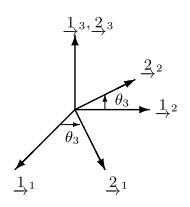
\includegraphics[width=.33\textwidth]{Img/RotationInX.png}}
%     \hfill
%     \subfloat[Rotación alrededor de $y$]{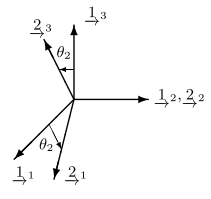
\includegraphics[width=.33\textwidth]{Img/RotationInY.png}}
%     \hfill
%     \subfloat[Rotación alrededor de $x$]{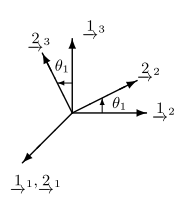
\includegraphics[width=.33\textwidth]{Img/RotationInZ.png}}
%     \caption{Rotaciones principales}
%     \label{fig:rotations_old}
% \end{figure}

\begin{figure}
    \centering
    \subfloat[Rotación alrededor de $x$]{\tdplotsetmaincoords{50}{140}
\begin{tikzpicture}[scale=2,tdplot_main_coords]
    \draw[thick,->] (0,0,0) -- (1,0,0) node[anchor=north east]{$x$};
    \draw[thick,->] (0,0,0) -- (0,1,0) node[anchor=north west]{$y$};
    \draw[thick,->] (0,0,0) -- (0,0,1) node[anchor=south]{$z$};
    
    \pgfmathsetmacro{\ax}{-.75}
    \pgfmathsetmacro{\ay}{2.5}
    \pgfmathsetmacro{\az}{0}
    
    \tdplotsetrotatedcoords{20}{40}{00}
    
    \draw[thick,color=red,tdplot_rotated_coords,->] (0,0,0) -- (.7,0,0) node[anchor=east]{$x’$};
    \draw[thick,color=green!50!black,tdplot_rotated_coords,->] (0,0,0) -- (0,.7,0) node[anchor=west]{$y’$};
    \draw[thick,color=blue,tdplot_rotated_coords,->] (0,0,0) -- (0,0,.7) node[anchor=south]{$z’$};
    
    \tdplottransformrotmain{\ax}{\ay}{\az}
    
    \draw[tdplot_main_coords,->,blue!50] (0,0,0) -- (\tdplotresx,\tdplotresy,\tdplotresz);
    \node[tdplot_rotated_coords,anchor=north] at (\ax,\ay,\az){Rotated coords: (\ax, \ay, \az)};
    \node[tdplot_main_coords,anchor=south] at (\tdplotresx,\tdplotresy,\tdplotresz){Main coords: (\tdplotresx, \tdplotresy, \tdplotresz)};

\end{tikzpicture}}
    \quad
    \subfloat[Rotación alrededor de $y$]{\tdplotsetmaincoords{50}{140}
\begin{tikzpicture}[scale=4,baseline,tdplot_main_coords]
    \coordinate (O) at (0,0,0);
    
    \draw[thick,->] (0,0,0) -- (1,0,0) node[anchor=north west]{$x$};
    \draw[thick,->] (0,0,0) -- (0,1,0) node[anchor=north west]{$y$};
    \draw[thick,->] (0,0,0) -- (0,0,1) node[anchor=north west]{$z$};
    
    \pgfmathsetmacro{\ax}{2}
    \pgfmathsetmacro{\ay}{2}
    \pgfmathsetmacro{\az}{1}
    
    \tdplotsetrotatedcoords{20}{20}{0}
    
    \draw[->,tdplot_rotated_coords,red] (0,0,0) -- (.7,0,0) node[anchor=south]{$x'$};
    \draw[->,red] (0,0,0) -- (0,1,0) node[anchor=north east]{$y'$};
    \draw[->,tdplot_rotated_coords,red] (0,0,0) -- (0,0,1) node[anchor=north east]{$z'$};
    
    \tdplotgetpolarcoords{\ax}{\ay}{\az}
    
    \tdplotsetthetaplanecoords{\tdplotresphi}
    
    % \tdplotdrawarc[tdplot_rotated_coords]{(0,0,0)}{1}{0}%
    % % tdplotdrawarc[tdplot_rotated_coords]{(0,0,0)}{1}{0}%
    % {\tdplotrestheta}{anchor=west}{$\theta = \tdplotrestheta$}
    \tdplotdrawarc{(0,0,0)}{0.5}{230}{241}{anchor=south}{$\theta_2$}
    \tdplotdrawarc{(0,0,0)}{0.5}{0}{30}{anchor=north east}{$\theta_2$}
    
\end{tikzpicture}}
    \quad
    \subfloat[Rotación alrededor de $z$]{\tdplotsetmaincoords{50}{140}
\begin{tikzpicture}[scale=4,baseline,tdplot_main_coords]
    \coordinate (O) at (0,0,0);
    
    \draw[thick,->] (0,0,0) -- (1,0,0) node[anchor=north east]{$x$};
    \draw[thick,->] (0,0,0) -- (0,1,0) node[anchor=north west]{$y$};
    \draw[thick,->] (0,0,0) -- (0,0,1) node[anchor=north west]{$z$};
    
    \pgfmathsetmacro{\ax}{2}
    \pgfmathsetmacro{\ay}{2}
    \pgfmathsetmacro{\az}{1}
    
    \tdplotsetrotatedcoords{20}{20}{0}
    
    \draw[->,tdplot_rotated_coords,red] (0,0,0) -- (.7,0,0) node[anchor=north east]{$x'$};
    \draw[->,tdplot_rotated_coords,red] (0,0,0) -- (0,.7,0) node[anchor=north west]{$y'$};
    \draw[->,red] (0,0,0) -- (0,0,\az) node[anchor=north east]{$z'$};
    
    \tdplotgetpolarcoords{\ax}{\ay}{\az}
    
    \tdplotsetthetaplanecoords{\tdplotresphi}
    
    % \tdplotdrawarc[tdplot_rotated_coords]{(0,0,0)}{1}{0}%
    % % tdplotdrawarc[tdplot_rotated_coords]{(0,0,0)}{1}{0}%
    % {\tdplotrestheta}{anchor=west}{$\theta = \tdplotrestheta$}
    \tdplotdrawarc{(0,0,0)}{0.5}{0}{30}{anchor=north}{$\theta_3$}
    \tdplotdrawarc{(0,0,0)}{0.5}{90}{110}{anchor=north west}{$\theta_3$}
    
\end{tikzpicture}}
    \caption{Rotaciones principales}
    \quad
    \label{fig:rotations}
\end{figure}

La matriz de rotación para el caso de la Figura \ref{fig:rotations}.a, el cual corresponde a una sobre el eje $x$, es
\begin{equation}
    \bm{C}_1 = 
    \begin{bmatrix}
        1 & 0 & 0 \\
        0 & \cos \theta_1 & \sin \theta_1 \\
        0 & -\sin \theta_1 & \cos \theta_1
    \end{bmatrix}
\end{equation}

En cambio, la matriz de rotación para el eje $y$, como se aprecia en la Figura \ref{fig:rotations}.b,
\begin{equation}
    \bm{C}_2 = 
    \begin{bmatrix}
        \cos \theta_2 & 0 & - \sin \theta_2 \\
        0 & 1 & 0 \\
        \sin \theta_2 & 0 & \cos \theta_2
    \end{bmatrix}
\end{equation}

Finalmente, la rotación en $z$ vista en la Figura \ref{fig:rotations}.c

\begin{equation}
    \bm{C}_3 = 
    \begin{bmatrix}
        \cos \theta_3 & \sin \theta_3 & 0 \\
        -\sin \theta_3 & \cos \theta_3 & 0 \\
        0 & 0 & 1
    \end{bmatrix}
\end{equation}


\subsubsection{Ángulos de Euler}
La orientación de un marco de referencia respecto a otro puede, también, ser especificada como una secuencia de tres rotaciones principales. Dependiendo el orden con el que se hagan dichas rotaciones, se conseguirán resultados distintos. Esto es debido a que las rotaciones en tres dimensiones no pertenecen a un espacio vectorial (y, por lo tanto, no pueden ser representadas por una), y suele considerárselas como un \textit{grupo}, el cual es una abstracción matemática. %Existen dentro de la literatura numerosos textos que tratan el tema, como pueden ser \textbf{PONER COSAS QUE HABLEN DE SO(3) SU(2) ETC ETC}.

En concreto, una secuencia muy utilizada en aplicaciones aeroespaciales realiza
\begin{enumerate}
    \item Una rotación $\theta_1$ sobre el eje original $1$ (rotación en ''roll'')
    \item Una rotación $\theta_2$ sobre el eje intermedio $2$ (rotación en ''pitch'')
    \item Una rotación $\theta_3$ sobre el eje transformado $3$ (rotación en ''yaw'')
\end{enumerate}
la cual suele ser llamada la secuencia 1-2-3 de actitud o la convención ''roll-pitch-yaw''. En este caso, la matriz de rotación del marco 1 al marco 2 está dada por
\begin{align}
    \bm{C}_{21}(\theta_3,\theta_2,\theta_1) &= \bm{C}_3(\theta_3)\bm{C}_2(\theta_2)\bm{C}_1(\theta_1) \\
    &=
    \begin{bmatrix}
        c_2c_3 & c_1s_3+s_1s_2c_3 & s_1s_3 - c_1s_2c_3 \\
        -c_2s_3 & c_1c_3 - s_1s_2s_3 & s_1c_3 + c_1s_2s_3 \\
        s_2 & -s_1c_2 & c_1c_2
    \end{bmatrix}
    \label{eq:rpyrotation}
\end{align}
donde $s_i = \sin{\theta_i}$ y $c_i = \cos{\theta_i}$.

Todas las secuencias de Euler tienen singularidades. Para la secuencia 1-2-3, una singularidad existe en $\theta_2 = \pi/2$. En este caso,

\begin{equation}
    \bm{C}_{21}(\theta_3,\frac{\pi}{2},\theta_1) = 
    \begin{bmatrix}
        0 & \sin{(\theta_1 + \theta_3)} & -\cos{(\theta_1 + \theta_3)} \\
        0 & \cos{(\theta_1 + \theta_3)} & \sin{(\theta_1 + \theta_3)} \\
        1 & 0 & 0
    \end{bmatrix}
\end{equation}

Por lo tanto, $\theta_1$ y $\theta_3$ se asocian con la misma rotación. Sin embargo, esto es solo un problema si se quieren recuperar los ángulos de  rotación de la matriz de rotación.

\paragraph{Rotaciones infinitesimales} Si los ángulos $\theta_1$, $\theta_2$, $\theta_3$ son pequeños, puede aproximarse que $c_i \approx 1$, $s_i \approx \theta_i$ y que, por ende, $\theta_i\theta_j$ es despreciable respecto a $1$. Entonces, para la transformación 1-2-3, la Expresión (\ref{eq:rpyrotation}) resulta
\begin{equation}
    \bm{C}_{21} \approx
    \begin{bmatrix}
        1 & \theta_3 + \theta_1\theta_2 & \theta_1\theta_3 - \theta_2 \\
        -\theta_3 & 1 & \theta_1 + \theta_2\theta_3 \\
        \theta_2 & -\theta_1 & 1
    \end{bmatrix}
    \label{eq:rpyinfinitesimal}
\end{equation}
ya que $\theta_1\theta_2$ es despreciable respecto a $1$.

Si además se desprecian los productos de ángulos pequeños $\theta_i\theta_j \approx 0$
\begin{align}
    \bm{C}_{21} &\approx
    \begin{bmatrix}
        1 & \theta_3 & -\theta_2 \\
        -\theta_3 & 1 & \theta_1 \\
        \theta_2 & -\theta_1 & 1
    \end{bmatrix}
    \label{eq:rpyinfinitesimalreduced}
    \\
    &\approx \bm{1} - \left[\bm{\theta}\right]_\times
\end{align}
siendo $\bm{\theta}$ el \textit{vector de rotación}, donde
\begin{align}
    \bm{\theta} &=
    \begin{bmatrix}
        \theta_1 \\
        \theta_2 \\
        \theta_3
    \end{bmatrix}
    \\
    \left[\bm{a}\right]_\times &= 
    \begin{bmatrix}
        0 & -a_z & a_y \\
        a_z & 0 & -a_x \\
        -a_y & a_x & 0
    \end{bmatrix}
\end{align}

\subsubsection{Cuaterniones}
Un cuaternión es una extensión de los números complejos, con tres raíces cuadradas de $-1$ ($ijk$) en lugar de solo una ($i$). Un cuaternión puede ser representado como un vector cuatridimensional de longitud unitaria, donde la primer componente es un número escalar real, mientras que las otras tres componentes forman un vector en el espacio $ijk$ siguiendo la regla de la mano derecha. 
\begin{equation}
    \bm{q} = q_w + q_i i + q_j j + q_k = q_w k = q_w \bm{q}_v
\end{equation}
siendo $q_w$ la \textit{parte real} y $\bm{q}_v$ a la \textit{parte vectorial}, cumpliéndose que
\begin{equation}
    i^2=j^2=k^2=ijk=-1
\end{equation}

Usualmente, se representa al mismo como un vector $\bm{q}$ de cuatro componentes
\begin{equation}
    \bm{q} =
    \begin{bmatrix}
    q_w \\
    \bm{q}_v
    \end{bmatrix}
\end{equation}
y al ser de interés en este trabajo los cuaterniones para expresar rotaciones, los mismos son \textit{unitarios} o \textit{normalizados}
\begin{align}
    \bm{q}(\hat{\bm{u}},\phi) =
    \begin{bmatrix}
    q_w(\phi) \\
    \bm{q}_v(\hat{\bm{u}},\phi)
    \end{bmatrix}
    &=
    \begin{bmatrix}
        \cos{\frac{\phi}{2}} \\
        \hat{\bm{u}}\sin{\frac{\phi}{2}}
    \end{bmatrix}
    \\
    ||\bm{q}(\hat{\bm{u}},\phi)|| &= 1
\end{align}

% \textbf{PONER O NO ESTO?????}
% En otras palabras, dicho cuaternión parametriza una rotación sobre un eje definido por el vector $\hat{\bm{u}}$, y un ángulo $\phi$ sobre ese vector, como puede verse en la Figura \ref{fig:quaternions}.
% \begin{figure}
%     \centering
%     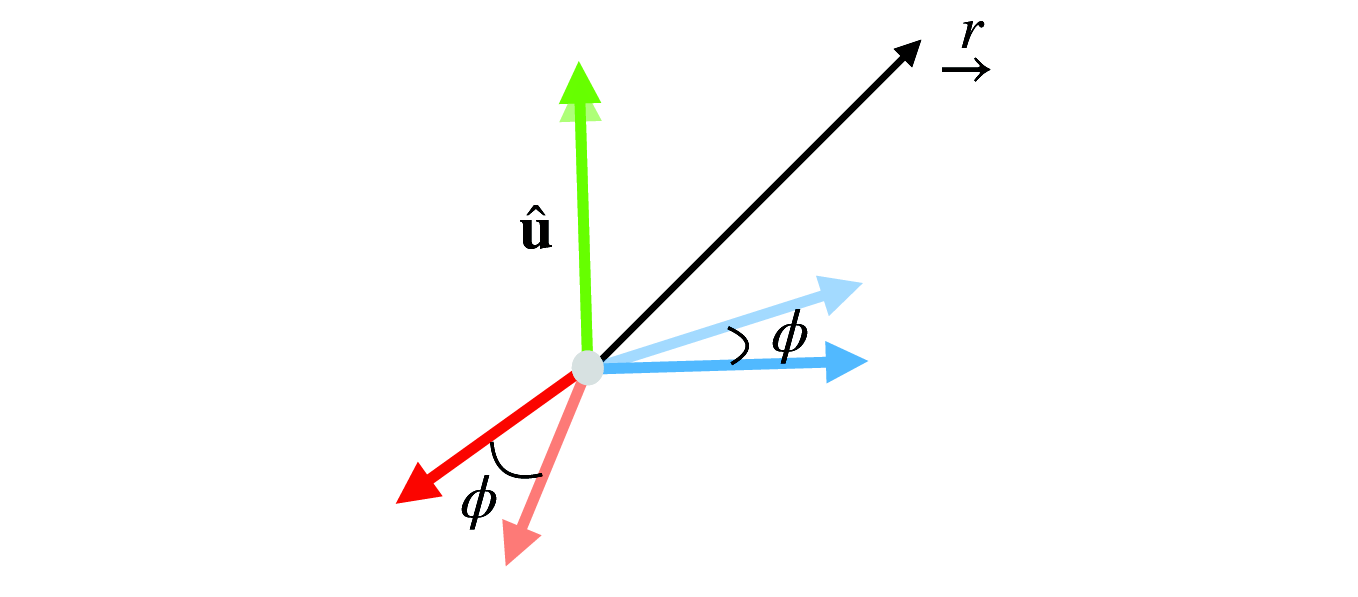
\includegraphics[width=\textwidth]{Img/Quaternions.png}
%     \caption{Rotación sobre un eje definido?}
%     \label{fig:quaternions}
% \end{figure}

\paragraph{Propiedades de los cuaterniones}
A continuación, se evaluarán algunas de las propiedades de los cuaterniones.
\subparagraph{Suma}
Tanto la suma como la resta son de forma directa
\begin{equation}
    \bm{p} \pm \bm{q} =
    \begin{bmatrix}
        p_w + q_w \\
        \bm{p}_v + \bm{q}_v
    \end{bmatrix}
\end{equation}

La suma, entonces, es \textit{conmutativa} y \textit{asociativa}
\begin{align}
    \bm{p} + \bm{q} &= \bm{q} + \bm{p} \\
    \bm{p} + (\bm{q} + \bm{s}) &= (\bm{p} + \bm{q}) + \bm{s}
\end{align}

\subparagraph{Producto}
Denotado con $\otimes$, el producto resulta
\begin{equation}
    \bm{p}\otimes\bm{q} = 
    \begin{bmatrix}
        p_wq_w - p_xq_x - p_yq_y - p_zq_z \\
        p_wq_x + p_xq_w + p_yq_z - p_zq_y \\
        p_wq_y - p_xq_z + p_yq_w + p_zq_x \\
        p_wq_z + p_xq_y - p_yq_x + p_zq_w
    \end{bmatrix}
\end{equation}

Por inspección, puede escribirse como un producto matricial
\begin{align}
    \bm{p}\otimes\bm{q} &= 
    \begin{bmatrix}
        q_w & -q_x & -q_y & -q_z \\
        q_x & q_w & q_z & -q_y \\
        q_y & -q_z & q_w & q_x \\
        q_z & q_y & -q_x & q_w
    \end{bmatrix}
    \begin{bmatrix}
        p_w \\
        p_x \\
        p_y \\
        p_z
    \end{bmatrix}
    \\
    &= 
    [\bm{q}]_R \bm{p}
    \label{eq:quaternionproductright}
\end{align}
y de forma análoga
\begin{align}
    \bm{p}\otimes\bm{q} &= 
    \begin{bmatrix}
        p_w & -p_x & -p_y & -p_z \\
        p_x & p_w & -p_z & p_y \\
        p_y & p_z & p_w & -p_x \\
        p_z & -p_y & p_x & p_w
    \end{bmatrix}
    \begin{bmatrix}
        q_w \\
        q_x \\
        q_y \\
        q_z
    \end{bmatrix}
    \\
    &= [\bm{p}]_L\bm{q}
    \label{eq:quaternionproductleft}
\end{align}
donde se definen a las matrices de producto de cuaterniones izquierda y derecha como
\begin{align}
    [\bm{q}]_R &= q_w\bm{I} +
    \begin{bmatrix}
        0 & -\bm{q_v}^T \\
        \bm{q}_v & -[\bm{q}_v]_\times
    \end{bmatrix}
    \label{eq:quaternionproductmatrixright}
    \\
    [\bm{q}]_L &= q_w\bm{I} +
    \begin{bmatrix}
        0 & -\bm{q_v}^T \\
        \bm{q}_v & [\bm{q}_v]_\times
    \end{bmatrix}
    \label{eq:quaternionproductmatrixleft}
\end{align}

El producto, entonces, es \textit{no conmutativo} en el caso general. Sin embargo, es \textit{asociativo}, además de \textit{distributivo sobre la suma}
\begin{align}
    \bm{p}\otimes\bm{q} &\neq \bm{q}\otimes\bm{p} \\
    (\bm{p}\otimes\bm{q})\otimes\bm{s} &= \bm{p}\otimes(\bm{q}\otimes\bm{s}) \\
    \bm{p}\otimes(\bm{q} + \bm{s}) &= \bm{p}\otimes\bm{q} + \bm{p}\otimes\bm{s} \\
    (\bm{p} + \bm{q})\otimes\bm{s} &= \bm{p}\otimes\bm{s} + \bm{q}\otimes\bm{s}
\end{align}
\subparagraph{Conjugado}
El conjugado de un cuaternión se define como
\begin{equation}
    \bm{q}^* = q_w - \bm{q_v}
\end{equation}
y tiene las propiedades de
\begin{align}
    \bm{q}\otimes\bm{q}^* = \bm{q^*}\otimes\bm{q} &= q_w^2 + q_x^2 + q_y^2 + q_z^2 \\
    (\bm{p}\otimes\bm{q})^* &= \bm{q}^*\otimes\bm{p}^*
\end{align}

\subparagraph{Norma}
La norma se define como
\begin{equation}
    ||\bm{q}|| = \sqrt{\bm{q}\otimes\bm{q}^*} = \sqrt{q_w^2 + q_x^2 + q_y^2 + q_z^2}
\end{equation}
y tiene la propiedad de
\begin{equation}
    ||\bm{p}\otimes\bm{q}|| = ||\bm{q}\otimes\bm{p}|| = ||\bm{p}|| \ ||\bm{q}||
\end{equation}

\subparagraph{Inversa}
La inversa de un cuaternión es aquella que si se realiza la multiplicación del cuaternion con la misma se obtiene la identidad.
\begin{equation}
    \bm{q}\otimes\bm{q}^{-1} = \bm{q}^{-1}\otimes\bm{q} = 1
    \label{eq:quaternioninverse}
\end{equation}
cuya expresión es
\begin{equation}
    \bm{q}^{-1} = \frac{\bm{q}^*}{||\bm{q}||^2}
\end{equation}

Si se trata de un \textit{cuaternión unitario}, esto es, $||\bm{q}|| = 1$, entonces
\begin{equation}
    \bm{q}^{-1} = \bm{q}^*    
\end{equation}

\subparagraph{Conmutador}
El \textit{conmutador} de un cuaternión se define como
\begin{equation}
    [\bm{p},\bm{q}] = \bm{p}\otimes\bm{q} - \bm{q}\otimes\bm{p} = \bm{p}_v\otimes\bm{q}_v - \bm{q}_v\otimes\bm{p}_v = 2\bm{p}_v\times\bm{q}_v
    \label{eq:quaternioncommutator}
\end{equation}

\paragraph{Rotaciones con cuaterniones}
Si se tiene un vector en el marco $a$ definido como $\bm{r}_a$, y al mismo se lo quiere llevar al marco $b$, del cual solo se diferencia por una rotación, esto puede hacerse con un cuaternión $\bm{q}$ que describa esa rotación mediante
\begin{equation}
    \bm{r}_b = \bm{q}\otimes\bm{r}_a\otimes\bm{q}^{-1}
    \label{eq:quaternionvectorrotation}
\end{equation}
donde tanto $\bm{r}_a$ como $\bm{r}_b$ corresponden a los vectores expresados en su forma de cuaternión, esto es,
\begin{equation}
    \bm{r} = 
    \begin{bmatrix}
    0 \\
    \bm{r}
    \end{bmatrix}
    \label{eq:vectorquaternionform}
\end{equation}

De forma análoga, puede convertirse un cuaternión a una matriz de rotación utilizando
\begin{align}
    \bm{r}_b &= \bm{C}(\bm{q}_{ba})\bm{r}_a \\
    \bm{C}(\bm{q}) &= (q_w^2 - \bm{q}_v^T\bm{q}_v)\bm{1} + 2\bm{q}_v\bm{q}_v^T + 2q_w\left[\bm{q}_v\right]_\times
\end{align}

\subsubsection{Resumen}
El punto principal para darse cuenta de las diferentes representaciones de las rotaciones es que siempre hay solo tres grados de libertad. Aquellas que tienen más de tres parámetros deben tener restricciones asociadas para limitar el número de grados de libertad a tres. Las representaciones que tienen exactamente tres parámetros tienen singularidades asociadas. No existe una representación perfecta que sea mínima (es decir, que tenga solo tres parámetros) y que también esté libre de singularidades\cite{stuelpnagle1964}.% \textbf{[Stuelpnagel, 1964]}.

De las tres representaciones vistas, esto es, la \textit{matriz de rotación}, los \textit{ángulos de Euler} y los \textit{cuaterniones}, cada una tiene ventajas como desventajas, reflejadas en la Tabla (\ref{tab:rotationrepresentations}).

\begin{table}[!ht]
\centering
\begin{tabular}{c|c|c|c}
                        & \textbf{\begin{tabular}[c]{@{}c@{}}Matriz \\ de rotación\end{tabular}} &  \textbf{\begin{tabular}[c]{@{}c@{}}Ángulos \\ de Euler\end{tabular}} & \textbf{Cuaterniones} \\ \hline \hline
\textit{Expresión}      & $\bm{C}$   & $\{\theta_3,\theta_2,\theta_1\}$     & $\bm{q} = 
    \begin{bmatrix}
        \cos{\frac{\phi}{2}} \\
        \hat{\bm{u}}\sin{\frac{\phi}{2}}
    \end{bmatrix}$  \\ \hline
\textit{Parámetros}     & 9          & 3                  & 4                                             \\ \hline 
\textit{Restricciones}  & $\bm{C}\bm{C}^T = \bm{1}$ &    No & $||\bm{q}|| = 1$                        \\ \hline 
\textit{Singularidades} & No             & Si                       
              & No                   \end{tabular}
\caption{Resumen de las representaciones de rotaciones vistas}
\label{tab:rotationrepresentations}
\end{table}

\subsection{Poses}
Como se ha hablado anteriormente a la rotación, ahora se presenta a la notación de \textit{traslación}. Juntos, la traslación y rotación de un cuerpo se denomina \textit{pose}. Los problemas de estimación de la pose a menudo tienen que ver con la transformación de las coordenadas de un punto, $P$, entre un marco de vehículo en movimiento (en traslación y rotación) y un marco estacionario, como se muestra en la Figura \ref{fig:pose}.
% \begin{figure}[!b]
%     \centering
%     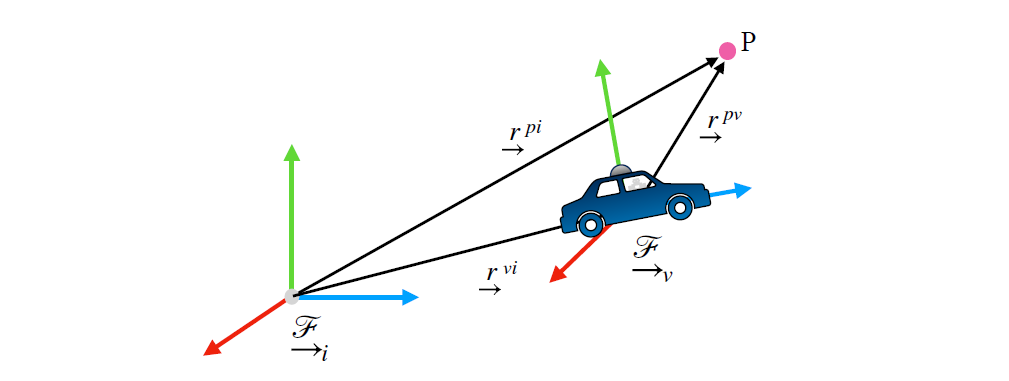
\includegraphics[width=\textwidth]{Img/Pose.png}
%     \caption{Estimación de la pose de un vehículo}
%     \label{fig:pose_old}
% \end{figure}

\begin{figure}
    \centering
    \tdplotsetmaincoords{60}{110}
\begin{tikzpicture}[scale=4,baseline,tdplot_main_coords]
    \draw[thick,->] (0,0,0) -- (.7,0,0) node[anchor=north east]{$\undervec{\bm{\mathcal{F}}}_i$};
    \draw[thick,->] (0,0,0) -- (0,.7,0);
    \draw[thick,->] (0,0,0) -- (0,0,.7);
    
    \coordinate (Shift) at (1,1.5,1);
    \coordinate (Point) at (2,2.4,3);
    \draw[thick,->,blue] (0,0,0) -- (Shift) node[midway,anchor=north west]{$\undervec{\bm{r}}^{vi}$};
    
    
    \draw[thick,->,blue] (0,0,0) -- (Point) node[midway,anchor=south east]{$\undervec{\bm{r}}^{pi}$};
    
    \draw[thick,->,blue] (Shift) -- (Point) node[midway,anchor=north west]{$\undervec{\bm{r}}^{pv}$};
    
    \draw[fill=black] (Point) circle (0.03) node[above right] {$p$};
    \tdplotsetrotatedcoords{20}{-10}{10}
    
    \tdplotsetrotatedcoordsorigin{(Shift)}
    
    \draw[thick,color=red,tdplot_rotated_coords,->] (0,0,0)-- (1,0,0) node[anchor=north east]{$\undervec{\bm{\mathcal{F}}}_v$};
    \draw[thick,color=red,tdplot_rotated_coords,->] (0,0,0)-- (0,.7,0);
    \draw[thick,color=red,tdplot_rotated_coords,->] (0,0,0)-- (0,0,.7);
    
\end{tikzpicture}
    \caption{Estimación de la pose de un vehículo}
    \label{fig:pose}
\end{figure}

Pueden relacionarse los vectores de dicha Figura como
\begin{equation}
    \undervec{r}^{pi} = \undervec{r}^{pv}+\undervec{r}^{vi}
\end{equation}
donde no fue elegido todavía ningún marco de referencia particular en el cual expresar la relación. Escribiendo la relación en el marco estacionario, $\undervec{\bm{\mathcal{F}}}_i$, se tiene
\begin{equation}
    \bm{r}_i^{pi} = \bm{r}_i^{pv} + \bm{r}_i^{vi}
\end{equation}

Si el punto $P$ se encuentra adjunto al vehículo, se conocen típicamente sus coordenadas en $\undervec{\bm{\mathcal{F}}}_v$, el cual está rotado respecto a $\undervec{\bm{\mathcal{F}}}_i$. Siendo $\bm{C}_{iv}$ la representación de esta rotación, puede reescribirse la relación como
\begin{equation}
    \bm{r}_i^{pi} = \bm{C}_{iv}\bm{r}_v^{pv} + \bm{r}_i^{vi}
    \label{eq:poseconvertion}
\end{equation}
que indica cómo convertir las cordenadas de $P$ en $\undervec{\bm{\mathcal{F}}}_v$ a las coordenadas de $\undervec{\bm{\mathcal{F}}}_i$, conociendo la traslación, $\bm{r}_i^{vi}$, y la rotación, $\bm{C}_{iv}$ entre los dos marcos. Finalmente, se refiere a la \textit{pose} del vehículo al conjunto
\begin{equation}
    \{\bm{r}_i^{vi},\bm{C}_{iv}\}
\end{equation}

\subsubsection{Matrices de transformación}
La Expresión (\ref{eq:poseconvertion}) puede reescribirse como
\begin{align}
    \begin{bmatrix}
        \bm{r}_i^{pi} \\
        1
    \end{bmatrix}
    &=
    \begin{bmatrix}
        \bm{C}_{iv} & \bm{r}_i^{vi} \\
        \bm{0}^T & 1
    \end{bmatrix}
    \begin{bmatrix}
        \bm{r}_v^{pv} \\
        1
    \end{bmatrix} \\
    &=
    \bm{T}_{iv}
    \begin{bmatrix}
        \bm{r}_v^{pv} \\
        1
    \end{bmatrix}
\end{align}
siendo $\bm{T}_{iv}$ una \textit{matriz de transformación} de $4x4$.

Para hacer uso de una matriz de transformación, es necesario agregar un $1$ a las coordenadas del punto, o sea
\begin{equation}
    \begin{bmatrix}
        x \\
        y \\
        z \\
        1
    \end{bmatrix}
\end{equation}
conocida como la representación \textit{homogénea} del punto. En este tipo de representación, cada entrada puede ser multiplicada por un \textit{factor de escala}, $s$
\begin{equation}
    \begin{bmatrix}
        sx  \\
        sy  \\
        sz  \\
        s
    \end{bmatrix}
\end{equation}

Para recuperar las coordenadas $(x,y,z)$ originales, es necesario dividir las primeras tres entradas por la cuarta. De este modo, mientras el factor de escala se aproxime a $0$, pueden representarse puntos arbitrariamente lejos del origen.

Para transformar las coordenadas de vuelta al otro lado, se necesita aplicar la inversa de la matriz de transformación
\begin{equation}
    \begin{bmatrix}
        \bm{r}_v^{pv} \\
        1
    \end{bmatrix}
    =
    \bm{T}_{iv}^{-1}
    \begin{bmatrix}
        \bm{r}_i^{pi} \\
        1
    \end{bmatrix}
\end{equation}
donde
\begin{equation}
    \bm{T}_{iv}^{-1} = \bm{T}_{vi}
\end{equation}

Además de esto, pueden realizarse matrices de transformación compuestas
\begin{equation}
    \bm{T}_{iv} = \bm{T}_{ia}\bm{T}_{ab}\bm{T}_{bv}
\end{equation}
lo que facilita encadenar un número arbitrario de cambios de pose juntos.

\subsubsection{Transformaciones en ROS}
Si, por ejemplo, se tiene un robot móvil dispuesto con un LIDAR y una unidad inercial, cada uno de estos sensores estarán en una cierta ubicación dentro del robot, la cual no necesariamente será en el centro del mismo, o en el punto \textit{base} elegido como centro de coordenadas del robot. Para poder relacionarlos, a cada uno de los sensores y componentes involucrados se les asocia un marco de referencia. Por ello, para poder asociar los datos de cada uno de estos sensores, es importante conocer la pose del marco de referencia de los mismos respecto a un punto o referencia en común como, por ejemplo, la base del robot.

Hay muchas formas de administrar marcos de coordenadas y transformaciones entre ellos. En ROS, continuando con la filosofía de mantener las cosas pequeñas y modulares, se trata de un enfoque distribuido, utilizando tópicos de ROS para compartir datos de transformación. Cualquier nodo puede ser la autoridad que publica la información actual para algunas transformaciones, y cualquier nodo puede suscribirse para transformar datos, obteniendo de todas las diversas autoridades una imagen completa del robot. Este sistema se implementa en el paquete \texttt{tf}\footnote{\url{http://wiki.ros.org/tf}}. Este paquete es relativamente complejo, y hay una variedad de formas en que las cosas pueden salir mal. En consecuencia, hay una serie de herramientas de depuración e introspección específicas de tf para ayudarlo a comprender lo que está sucediendo, desde imprimir una sola transformación en la consola hasta representar una vista gráfica de toda la jerarquía de transformación.

\subsection{Marcos de referencia}

% \begin{figure}
%     \centering
%     \subfloat[El marco \textit{e} en una cierta ubicación de la Tierra, el marco \textit{e} rotando con la Tierra, y el marco \textit{i}]{{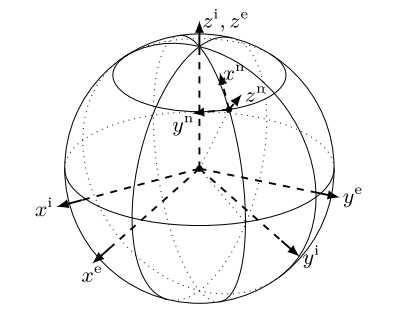
\includegraphics[width=0.47\textwidth]{Img/CoordinateFramesnei.png}}}%
%     \qquad
%     \subfloat[El marco \textit{s} del LIDAR dentro del robot móvil, y el marco \textit{b} en el centro de masa del mismo]{{\includegraphics[width=0.47\textwidth]{Img/CoordinateFramesbs.png}}}%
%     \caption{Marcos de referencia presentados}
%     \label{fig:coordinateframes}
% \end{figure}
Con el fin de poder combinar todos los sensores a utilizar con sus respectivas referencias para formar la estimación de estado y el mapa, es necesario introducir una serie de marcos de coordenadas:
\begin{itemize}
    \item \textbf{Marco del vehículo (vehicle frame)$\undervec{\bm{\mathcal{F}}}_v$ o marco del cuerpo (body frame)} $\undervec{\bm{\mathcal{F}}}_b$: Es el marco de coordenadas del robot en movimiento. Su origen suele encontrarse en el centro de masa.
    \item \textbf{Marco sensorial (sensor frame)} $\undervec{\bm{\mathcal{F}}}_s$: Adjunto rígidamente a un sensor como, por ejemplo, el LIDAR, GPS o la unidad inercial de medición. Para localización, se suele ignorar la diferencia entre el el marco del robot móvil y el sensorial, ya que se asume que si se puede rastrear al sensor, es posible entonces rastrear cualquier punto en el robot móvil con la calibración adecuada.
    \item \textbf{Marco de navegación (navigation frame)} $\undervec{\bm{\mathcal{F}}}_n$: es un marco geográfico local en el que se quiere navegar. En otras palabras, es de interés en la posición y orientación del marco $\undervec{\bm{\mathcal{F}}}_v$ con respecto a este marco. Para la mayoría de las aplicaciones se define estacionaria con respecto a la Tierra. Sin embargo, en los casos en que se espera que el sensor se mueva a grandes distancias, se acostumbra mover y rotar el marco $\undervec{\bm{\mathcal{F}}}_n$ a lo largo de la superficie de la Tierra. Un marco de navegación típico es aquel que se encuentra adjunto a un punto de partida pertinente, y se encuentra alineado con el Norte, Este y Abajo (NED, de sus siglas en inglés).
    \item \textbf{Marco inercial (inertial frame)} $\undervec{\bm{\mathcal{F}}}_i$: Es un marco estacionario. La unidad inercial de medición, por ejemplo, mide la aceleración lineal y la velocidad angular con respecto a este marco. Su origen se encuentra en el centro de la Tierra y sus ejes $x$ e $y$ se encuentran fijos respecto a las estrellas distantes, mientras que el eje $z$ apunta al Norte verdadero. Esto quiere decir que, aunque la Tierra gire alrededor del eje $z$, los ejes $x$ e $y$ no se mueven.
    \item \textbf{Marco de la Tierra (Earth frame)} $\undervec{\bm{\mathcal{F}}}_e$: Coincide con el marco $\undervec{\bm{\mathcal{F}}}_i$, pero gira con la Tierra. Es decir, tiene su origen en el centro de la Tierra y los ejes que se fijan con respecto a la Tierra. En particular, el eje $x$ se alinea con el Ecuador, el eje $y$ está asociado a la regla de la mano derecha, y el eje $z$ apunta al Norte verdadero.
\end{itemize}

% Las coordenadas correspondientes a los marcos de la Tierra, de navegación e inercial pueden observarse en la Figura \ref{fig:coordinateframes}.a, mientras que las correspondientes al marco sensorial de, por ejemplo, un LIDAR, y al marco del vehículo se observan en la Figura \ref{fig:coordinateframes}.b. Estos serán de relevancia en las siguientes secciones.
    \newpage
    % Regression analysis o state estimation?
\section{Estimación de estado}
La estimación de estado consiste en determinar el estado no medible de un sistema dinámico a partir de las mediciones de entrada y salida de dicho sistema. Lamentablemente, las mediciones no son perfectas, lo que conduce a una inexactitud inherente en el valor de la medición. Para tener en cuenta estos errores, la estimación de estado procesa todas las mediciones disponibles y utiliza un \textit{análisis de regresión} para identificar el estado real probable del sistema.

El análisis de regresión es un análisis estadístico para predecir el valor de una variable cuantitativa continua. Basándose en un conjunto de variables independientes, se busca estimar la relación de las mismas con una variable dependiente, mediante la obtención de una curva que mejor se ajuste a los datos disponibles, sin que necesariamente pase por todos ellos. En concreto, el modelo de regresión puede representarse como
\begin{equation}
    y_i = f(\bm{x}_i; \bm{\beta}) + v_i,
    \label{eq:regressionmodel}
\end{equation}
donde la variable $y_i$ corresponde a la respuesta o medición para el caso $i$, con $i = 1, 2, ..., m$, $\bm{x}_i = (x_{i1}, x_{i2}, ..., x_{in})$ corresponde al conjunto de valores, fijos o aleatorios, utilizados para explicar o predecir el comportamiento de $y_i$, conocidos como las \textit{variables regresivas} o independientes, $\bm{\beta} = (\beta_1, \beta_2, ..., \beta_n)$ a los parámetros desconocidos\footnote{A diferencia de un estado, el que se define como una magnitud física que varía a través del tiempo, el parámetro es constante a través del tiempo.} a estimar, y $v_i$ a la componente de ruido propia para ese caso.

En base a esto, lo que se busca es estimar la función $f$ que mejor se ajuste a los datos, conocida como \textit{función de expectativa} para el modelo de regresión. Para ello, primero lo que debe hacerse es determinar la forma de dicha función. En base a la forma que adquiera la misma, se puede clasificar en \textit{regresión lineal} y \textit{regresión no lineal}.

Existen diferentes métodos dentro del análisis de regresión para poder estimar los parámetros desconocidos $\beta$, por lo que en las siguientes subsecciones se presentarán algunos de ellos, los cuales son de relevancia para el seguimiento de la tesis.

% En cambio, cuando la función que modela al sistema \textit{no puede expresarse como una combinación lineal de los parámetros desconocidos} $\bm{\beta}$, se trata entonces de una regresión no lineal, y debe realizarse un proceso iterativo para encontrar la curva que mejor se adapte al sistema.

% La información de tales relaciones se efectúa a partir de información muestral acerca de los valores tomados por $y$, $x_1$, $x_2$, $x_3$, ..., $x_n$, y trata de cuantificar la magnitud de la dependencia entre ellas.

\subsection{Regresión lineal}
En regresión lineal, la variable $y$ \textit{es una combinación lineal} de los parámetros, es decir,
\begin{align}
    y_i &= \beta_1 x_{i1} + \beta_2 x_{i2} + \beta_3 x_{i3} + ... + \beta_n x_{in} + v_i \\
      &= \bm{x}_i \bm{\beta} + v_i
\end{align}

Con el fin de hallar los parámetros desconocidos, uno de los métodos más utilizados corresponde al \textit{método de cuadrados mínimos}, el cual plantea que el valor más probable de los parámetros desconocidos será aquel que minimiza la suma de los errores cuadráticos entre lo que se observa y lo que se espera. Este método es una variante especial del problema más general, en el que dada una función $f:\mathbb{R}^n\rightarrow\mathbb{R}$ se busca un argumento de $f$ que de el mínimo valor de la llamada \textit{función de coste}
\begin{equation}
    \hat{x} = argmin_x f(x)
    \label{eq:globalminimizer}
\end{equation}
llamado tambien como el \textit{minimzador global}.

\subsubsection{Cuadrados mínimos ordinario}
Si se quiere, por ejemplo, medir el peso de una bolsa de naranjas, cuyo valor real es $x$, con el uso de una balanza de poca precisión, el valor medido $y$ puede modelarse como el valor real corrompido por ruido, $v$, linealmente mediante la ecuación
\begin{equation}
    y = x + v
    \label{eq:linearmeasmodel}
\end{equation}

Para cada una de las mediciones, se define un término escalar de ruido que es independiente de los otros términos de error ya que, para este caso, se asume que el ruido es independiente y de distribución uniforme. Ahora, si se define el error entre cada medición y el valor verdadero de la bolsa de naranjas, se obtiene el denominado \textit{criterio de error} de cada medición, esto es,
\begin{equation}
    e_i = y_i - x
\end{equation}

Con estos errores definidos, el método de cuadrados mínimos define que la mejor estimación del valor $x$ es la que minimiza el \textit{criterio de error cuadrático},
\begin{equation}
    \hat{x}_{LS} = argmin_x(e_1^2+e_2^2+e_3^2+e_4^2+e_5^2) = \mathscr{L}_{LS}(x),
    \label{eq:squarederrorcriterion}
\end{equation}
aunque a veces también llamada \textit{función de coste de error cuadrático} o \textit{función de pérdida}.

% Luego de un set de cinco mediciones realizadas por separado y en forma secuencial, se obtienen los valores que se observan en la Tabla \ref{tab:naranjasbalanza}, junto con sus modelos de medición y errores cuadráticos.

% \begin{table}[]
\centering
\begin{tabular}{c|c|c|c}
\textbf{Medición} & \textbf{Peso {[}g{]}} & \textbf{Modelo de medición} & \textbf{Error} \\ \hline
1                       & 1012                  & $y_1 = x + v_1$        & $e_1 = y_1 - x$      \\ \hline
2                       & 989                   & $y_2 = x + v_2$        & $e_2 = y_2 - x$      \\ \hline
3                       & 1008                  & $y_3 = x + v_3$        & $e_3 = y_3 - x$      \\ \hline
4                       & 1030                  & $y_4 = x + v_4$        & $e_4 = y_4 - x$      \\ \hline
5                       & 971                   & $y_5 = x + v_5$        & $e_5 = y_5 - x$           
\end{tabular}
\caption{Peso de una bolsa de naranjas para cada medición realizada}
\label{tab:naranjasbalanza}
\end{table}

Para poder minimizar la función de coste, suponiendo que fueron tomadas cinco mediciones realizadas por separado y en forma secuencial, primero hay que reescribir a la función de error en su forma matricial, siendo entonces
\begin{align}
    \bm{e} &= \bm{y} - \bm{H}\cdot x \\
    \begin{bmatrix}
        e_1\\ e_2\\ e_3\\ e_4\\ e_5
    \end{bmatrix}
    &= 
    \begin{bmatrix}
        y_1\\ y_2\\ y_3\\ y_4\\ y_5
    \end{bmatrix}
    -
    \begin{bmatrix}
        1\\ 1\\ 1\\ 1\\ 1
    \end{bmatrix}
    x
\end{align}
siendo $\bm{H}$ la \textit{matriz Jacobiana}. Dicha matriz tiene las dimensiones de $m\times n$, donde \textit{m} es el número de mediciones y \textit{n} es el número de parámetros que se desean estimar. Por ello, \textit{x} si bien en este caso es un escalar, puede ser un vector en el caso que se tengan múltiples indeterminaciones. En base a esto, se puede redefinir a la función de costo como

\begin{align}
    \mathscr{L}_{LS}(x) &= \bm{e}^T\bm{e} \\
                        &= (\bm{y} - \bm{H}x)^T(\bm{y} - \bm{H}x) \\
                        &= \bm{y}^T\bm{y} - x^T\bm{H}^T\bm{y} - \bm{y}^T\bm{H}x + x^T\bm{H}^T\bm{H}x
\end{align}

Para minimizar esta ecuación, se procede a computar la derivada parcial de la función de costo respecto a la incertidumbre $x$ para luego igualarla a cero.
\begin{align}
    \frac{\partial \mathscr{L}}{\partial x}\bigg\rvert_{x=\hat{x}} = -\bm{y}^T\bm{H} - \bm{y}^T\bm{H} + 2\hat{x}^T\bm{H}^T\bm{H} &= 0 \\
    -2\bm{y}^T\bm{H} + 2\hat{x}^T\bm{H}^T\bm{H} &= 0
\end{align}

Despejando, se llega al valor del peso de la bolsa de naranjas que minimiza el criterio de error cuadrático
\begin{equation}
    \hat{x}_{LS} = (\bm{H}^T\bm{H})^{-1}\bm{H}^T\bm{y}
\end{equation}

Esta expresión tiene solución si y solo si existe $(\bm{H}^T\bm{H})^{-1}$, o sea, si la matriz tiene inversa. Si tenemos \textit{m} mediciones y \textit{n} parámetros,
\begin{align*}
    \bm{H} &\in \Re^{m\times n} \\
    \bm{H}^T\bm{H} &\in \Re^{n\times n}
\end{align*}

Por lo tanto, para que $(\bm{H}^T\bm{H})^{-1}$ exista es necesario que se dispongan mínimamente de la misma cantidad de mediciones que variables a estimar, esto es
\begin{equation*}
    m \geq n
\end{equation*}

\subsubsection{Cuadrados mínimos ponderado}

Volviendo al ejemplo de la bolsa de naranjas, si se toman mediciones con distintas balanzas, es lógico pensar que mientras mayor sea la precisión de cada una, mayor importancia tendrá su valor indicado para determinar el peso de la bolsa. Si se considera al modelo de medición lineal con \textit{m} mediciones y \textit{n} incertidumbres,
\begin{align}
    \begin{bmatrix}
        y_1 \\ . \\ . \\ . \\ y_m
    \end{bmatrix}
    &=
    \bm{H}
    \begin{bmatrix}
        x_1 \\ . \\ . \\ . \\ x_n
    \end{bmatrix}
    +
    \begin{bmatrix}
        v_1 \\ .\\ . \\ . \\ v_m
    \end{bmatrix} \\
    \bm{y} &= \bm{H} \bm{x} + \bm{v}
\end{align}

En cuadrados mínimos ordinarios, se asume implícitamente que cada término de error, $v_i$, posee el mismo desvío estándar, $\sigma$. En cambio, si se toma que cada término de error es independiente pero con distinto desvío estándar,
\begin{equation}
    \mathbb{E}_{[v_i^2]} = \sigma_i^2 \hspace{0.5cm}(i=1,...,m)\hspace{1cm}\bm{R}=\mathbb{E}_{[\bm{v}\bm{v}^T]} = 
    \begin{bmatrix}
        \sigma_1^2  &        &     0      \\
                    & \ddots &            \\
            0       &        & \sigma_m^2
    \end{bmatrix}
\end{equation}
se puede definir a partir de esto el \textit{criterio de cuadrados mínimos ponderado} como
\begin{align}
    \mathscr{L}_{WLS}(x) &= \bm{e}^T\bm{R}^{-1}\bm{e} \\
                         &= \frac{e_1^2}{\sigma_1^2} + \frac{e_2^2}{\sigma_2^2} + ... + \frac{e_m^2}{\sigma_m^2}
\end{align}

Mientras mayor sea el ruido esperado, menor será el peso que tenga en la medición. En el caso que todos los desvíos sean iguales, \textit{no afecta el valor estimado final}, ya que pasa a ser una constante dividiendo a todos los errores.

Expandiendo el nuevo criterio,
\begin{align}
    \mathscr{L}_{WLS}(x) &= \bm{e}^T\bm{R}^{-1}\bm{e} \\
                         &= (\bm{y} - \bm{H}\bm{x})^T\bm{R}^{-1}(\bm{y}-\bm{H}\bm{x})
\end{align}

Como en el caso de los cuadrados mínimos ordinarios, la ecuación MONGO puede minimizarse realizando el gradiente en este caso al ser que se cuentan con \textit{n} incógnitas.
\begin{equation}
    \frac{\partial \mathscr{L}}{\partial \bm{x}}\bigg\rvert_{\bm{x}=\hat{\bm{x}}} = -\bm{y}^T\bm{R}^{-1}\bm{H} + \hat{\bm{x}}^T\bm{H}^T\bm{R}^{-1}\bm{H} = 0
\end{equation}

obteniendo entonces las ecuaciones normales ponderadas
\begin{equation}
    \hat{\bm{x}}_{WLS} = (\bm{H}^T\bm{R}^{-1}\bm{H})^{-1} \bm{H}^T\bm{R}^{-1}\bm{y}
\end{equation}

\subsubsection{Cuadrados mínimos recursivo}

Hasta el momento, todos los datos de las mediciones se encontraban disponibles. Ahora, si lo que se tiene es, por ejemplo, un sensor que entrega datos cada cierto tiempo, con el razonamiento utilizado hasta el momento se tendería a pensar que es necesario correr alguno de los métodos vistos cada vez que llega un dato nuevo con todo el set completo. Se puede apreciar que claramente esto produciría un aumento de costo computacional a medida que transcurre el tiempo, haciendo que en un punto llegue a ser un problema.

Para evitar este problema, lo que se busca es un método recursivo que mantenga un estimador actual del parámetro óptimo para todas las mediciones que se han recolectado hasta ese momento, y luego actualizar dicho estimador dada la medición en el intervalo de tiempo actual. Para lograr esto, se puede utilizar entonces un \textit{estimador lineal recursivo}.

Suponiendo que se tiene un estimador óptimo $\hat{\bm{x}}_{k-1}$ de los parámetros desconocidos en el tiempo $k-1$ con ruido blanco Gaussiano aditivo. Al llegar la nueva medición en el tiempo $k$,
\begin{equation}
    \bm{y}_k = \bm{H}_k \bm{x} + \bm{v}_k
\end{equation}

Por lo tanto, el objetivo es poder computar $\hat{\bm{x}}_k$ como una función de $\bm{y}_k$ y $\hat{\bm{x}}_{k-1}$.

Un estimador lineal recursivo está dado por
\begin{equation}
    \hat{\bm{x}}_k = \hat{\bm{x}}_{k-1} + \bm{K}_k (\bm{y}_k - \bm{H}_k \hat{\bm{x}}_{k-1})
\end{equation}

donde $\bm{K}_k$ es una matriz de ganancia del estimador, el término entre paréntesis se denomina la innovación, y cuantifica que tan bien la medición actual se equipara con el mejor estimador previo. Aún sin conocer la matriz $\bm{K}_k$, en dicha ecuación puede observarse que el nuevo estimador es la suma del estimador anterior y el término correctivo basado en la diferencia entre lo esperado de la medición y lo que acutalmente se midió. Si la innovación fuese igual a cero, se mantendría el estimador anterior.

Finalmente, para el término $\bm{K}_k$, lo que se busca es minimizar el \textit{valor esperado de la suma de errores cuadráticos} del estimador actual en el tiempo \textit{k}. Para un solo parámetro escalar,
\begin{align}
    \mathscr{L}_{RLS}(x) &= \mathbb{E}_{[(x_k - \hat{x}_k)^2]} \\
                         &= \sigma_k^2
\end{align}

En cambio, si se tienen \textit{n} parámetros desconocidos en el tiempo \textit{k}
\begin{align}
    \mathscr{L}_{RLS}(x) &= \mathbb{E}_{[(x_{1k} - \hat{x}_{1k})^2 + ... + (x_{nk} - \hat{x}_{nk})^2]} \\
                         &= tr(\bm{P}_k)
\end{align}

siendo $tr()$ la \textit{traza} (o \textit{trace})\footnote{Corresponde a la suma de los elementos de la diagonal principal de la matriz} de la matriz de covarianza $\bm{P}_k$. En lugar de minimizar directamente el error, lo que se minimiza es su valor esperado, el cual es la varianza del estimador. A menor varianza, mayor será el grado de confianza del estimador.

Al igual que antes, es posible expresar a la covarianza en función de $\bm{K}_k$ utilizando la formulación lineal recursiva
\begin{equation}
    \bm{P}_k = (\bm{1} - \bm{K}_k\bm{H}_k)\bm{P}_{k-1}(\bm{1}-\bm{K}_k\bm{H}_k)^T + \bm{K}_k\bm{R}_k\bm{K}_k^T
\end{equation}

Mediante el uso de cálculo matricial y derivadas parciales, se puede llegar a que este término se minimiza cuando
\begin{equation}
    \bm{K}_k = \bm{P}_{k-1}\bm{H}_k^T(\bm{H}_k\bm{P}_{k-1}\bm{H}_k^T + \bm{R}_k)^{-1}
\end{equation}

En base a esto, es posible reescribir la ecuación de la matriz de covarianza como
\begin{align}
    \bm{P}_k &= \bm{P}_{k-1} - \bm{K}_k\bm{H}_k\bm{P}_{k-1} \\
                 &= (\bm{1} - \bm{K}_k\bm{H}_k)\bm{P}_{k-1}
\end{align}

De este último término se puede observar que cuanto más grande sea la matriz de ganancia $\bm{K}$, será más pequeña la nueva covarianza del estimador. Por lo tanto, se puede decir que la covarianza \textit{se encoge} con cada medición.

Resumiendo, el algoritmo de los cuadrados mínimos recursivos consta de tres pasos
\begin{enumerate}
    \item Inicializar los parámetros desconocidos y la matriz de covarianza. Esta predicción inicial, por ejemplo, puede obtenerse a partir de la primer medición que se toma y la covarianza puede venir de especificaciones técnicas.
        \begin{align}
            \hat{\bm{x}}_0 &= \mathbb{E}_{[\bm{x}]} \\
            \bm{P}_0 &= \mathbb{E}_{[(\bm{x} - \hat{\bm{x}}_0)(\bm{x} - \hat{\bm{x}}_0)^T]}
        \end{align}
    \item Definir el Jacobiano y la matriz de covarianza de la medición
        \begin{equation}
          \bm{y}_k = \bm{H}_k\bm{x}+\bm{v}_k
        \end{equation}
    \item Actualizar el valor estimado de $\hat{\bm{x}}_k$ y la covarianza $\bm{P}_k$
        \begin{align}
            \bm{K}_k &= \bm{P}_{k-1}\bm{H}_k^T(\bm{H}_k\bm{P}_{k-1}\bm{H}_k^T + \bm{R}_k)^{-1} \\
            \hat{\bm{x}}_k &= \hat{\bm{x}}_{k-1} + \bm{K}_k(\bm{y}_k - \bm{H}_k\hat{\bm{x}}_{k-1}) \\
            \bm{P}_k &= (\bm{1} - \bm{K}_k\bm{H}_k)\bm{P}_{k-1}
        \end{align}
\end{enumerate}

\subsubsection{Método de máxima verosimilitud}

En lugar de escribir una pérdida, puede aproximarse el problema de la estimación de parámetros óptimos al buscar qué parámetro hacen que las mediciones obtenidas sean las más probables. En otras palabras, cuál \textit{x} maximiza la probabilidad condicional de $\bm{y}$
\begin{equation}
    \hat{x} = argmax_x p(y|x)
\end{equation}

Volviendo al ejemplo de la bolsa de naranjas, si se tienen cuatro posibles valores de dicho peso, como se observa en la Figura \ref{fig:mostlikelyproba}, el valor que maximiza la verosimilitud condicional dada la medición $y_med$ corresponde a $x_b$, ya que es la densidad de probabilidad mayor en la ubicación medida.
\begin{figure}
    \centering
    \includegraphics[width=\textwidth]{Img/MostLikelyProba.png}
    \caption{Posibles valores del peso de la bolsa de naranjas y su valor real $y_{med}$}
    \label{fig:mostlikelyproba}
\end{figure}

Tomando en cuenta el modelo de medición presente en la Ecuación (\ref{eq:linearmeasmodel}), el mismo puede ser expresado como una probabilidad condicional de la medición, asumiendo alguna densidad de probabilidad para $v$, por ejemplo, ruido blanco Gaussiano aditivo
\begin{equation}
    v \sim \mathcal{N}(0,\sigma^2)
\end{equation}

entonces, el parámetro desconocido, $x$, resulta ser la media de esta densidad, y la varianza corresponde a la varianza de ruido.
\begin{equation}
    p(y|x) = \mathcal{N}(x,\sigma^2)
\end{equation}

Teniendo en cuenta que la función densidad de probabilidad de una Gaussiana es
\begin{equation}
    \mathcal{N}(z;\mu,\sigma^2) = \frac{1}{\sigma \sqrt{2\pi}} e^{\frac{-(z-\mu)^2}{2\sigma^2}}
\end{equation}

puede expresarse la medición de verosimilitud para una de las mediciones como
\begin{align}
    p(y|x) &= \mathscr{N}(y;x,\sigma^2) \\
           &= \frac{1}{\sqrt{2\pi\sigma^2}} e^{\frac{-(y-x)^2}{2\sigma^2}}
\end{align}

Si se tienen múltiples mediciones múltiples independientes, entonces
\begin{align}
    p(\bm{y}|x) &\propto \mathscr{N}(y_1;x,\sigma^2)\cdot\mathscr{N}(y_2;x,\sigma^2)\cdot...\cdot\mathscr{N}(y_m;x,\sigma^2) \\
            &= \frac{1}{\sqrt{(2\pi)^m\sigma^{2m}}} \exp\left({\frac{-\sum_{i=1}^m(y_i-x)^2}{2\sigma^2}}\right)
\end{align}

El estimador de máxima verosimilitud (MLE) está dado por
\begin{equation}
    \hat{x}_{MLE} = argmax_x p(\bm{y}|x)
\end{equation}

En lugar de tratar de optimizar el verosímil directamente, puede aplicarse el logaritmo
\begin{align}
    \hat{x}_{MLE} = argmax_x \log p(\bm{y}|x)
\end{align}

El logaritmo aumenta monotónicamente. Resulta entonces
\begin{equation}
    \log p(\bm{y}|x) = -\frac{1}{2\sigma^2}\left((y_1-x)^2+...+(y_m-x)^2\right)+C
\end{equation}

Esta ecuación es muy parecida a la suma de los errores cuadráticos. La constante $C$ en esta expresión refiere a términos que no son funciones de $x$ y pueden ser ignorados.

Luego, como el argmax de la función f es equivalente al argmin del negativo de dicha función, 
\begin{equation}
    argmax_z f(z) = argmin_z \left(-f(z)\right)
\end{equation}

el problema del verosímil máximo puede ser escrito como
\begin{align}
    \hat{x}_{MLE} &= argmin_x -\left(\log p(\bm{y}|x)\right) \\
                  &= argmin_x \frac{1}{2\sigma^2}\left((y_1-x)^2+...+(y_m-x)^2\right)
\end{align}

Por lo tanto, es posible realizar la maximización de la verosimilitud mediante una minimización de la suma de errores cuadráticos. Esto es válido ya que se asume que las mediciones se encuentran corrompidas por ruido blanco Gaussiano independiente aditivo de igual varianza.

Finalmente, si se asume que cada medición tiene una varianza distinta, se llega al mismo criterio que en cuadrados mínimos ponderados
\begin{equation}
    \hat{x}_{MLE} = argmin_x \frac{1}{2}\left(\frac{(y_1-x)^2}{\sigma_1^2}+...+\frac{(y_m-x)^2}{\sigma_m^2}\right)
\end{equation}

Resumiendo, en ambos casos, el estimador de máxima verosimilitud para ruido blanco Gaussiano es equivalente a las soluciones de los cuadrados mínimos ordinarios o ponderados.
\begin{equation}
    \hat{x}_{MLE} = \hat{x}_{LS} = argmin_x\mathscr{L}_{LS}(x) = argmin_x\mathscr{L}_{MLE}(x)
\end{equation}

Esto cobra importancia en sistemas realistas, los cuales presentan una gran cantidad de fuentes de ruido. Recordando el teorema central del límite, que establece que cuando se suman variables aleatorias independientes, su suma normalizada tenedrá a una distribución normal, y teniendo en cuenta que el método de cuadrados mínimos es equivalente a calcular la máxima verosimilitud\footnote{Siempre asumiendo que se está en presencia de ruido blanco Gaussiano aditivo}, es posible calcular el mejor estimador de una forma computacionalmente sencilla.

Sin embargo, una consideración importante a tener en cuenta con el método de cuadrados mínimos es cuando se presenta un valor atípico, esto es, los que se encuentran en las "colas" de la Gaussiana, provocando que el estimador final se aleje del valor verdadero. Por ello es importante cuantificar la distribución de error antes de aplicar ciegamente máxima verosimilitud o cuadrados mínimos.

\subsection{Regresión no lineal}

La regresión lineal es un método poderoso para analizar los datos descriptos por modelos que son lineales en los parámetros. Sin embargo, muchas veces las formas de las curvas que mejor ajustan a los datos obtenidos son no lineales en los parámetros. En estos casos, el modelo de regresión sigue siendo de la misma forma que el de la Expresión (\ref{eq:regressionmodel}), a diferencia de que al menos una de las derivadas de la función de expectativa con respecto a los parámetros depende de al menos uno de los parámetros\footnote{Por ejemplo, si derivo $\theta_1 \theta_2 x_1$ respecto a cualquiera de esos dos parámetros, dicha derivada parcial dependerá del parámetro no derivado}.

Para diferenciar entre modelos lineales y no lineales, los parámetros para este último caso se definen con $\bm{\theta}$,
\begin{equation}
    y_i = f(\bm{x}_i, \bm{\theta}) + v_i
    \label{eq:nonlinearregressionmodel}
\end{equation}

El criterio de error cuadrático para modelos no lineales es uno general, del cual puede derivarse la Expresión (\ref{eq:squarederrorcriterion})
\begin{align}
    \mathscr{S}(\bm{\theta}) &= \sum_{i=1}^n (y_i - f(\bm{x}_i;\bm{\theta}))^2 \\
                   &= (\bm{y} - \bm{f}(\bm{\theta}))^T\bm{R}^{-1}(\bm{y} - \bm{f}(\bm{\theta})) \\
                   &= \bm{y}^T \bm{R}^{-1}\bm{y} - 2\bm{y}^T\bm{R}^{-1}\bm{f}(\bm{\theta}) + \bm{f}(\bm{\theta})^T\bm{R}^{-1}\bm{f}(\bm{\theta})
    \label{eq:generalsquarederrorcriterion}
\end{align}
donde $\bm{f}(\bm{\theta}) = (f_1(\bm{\theta}), f_2(\bm{\theta}), ..., f_n(\bm{\theta}))$ y $f_i(\bm{\theta}) = f(\bm{x}_i;\bm{\theta})$.

A diferencia de la situación de cuadrados mínimos lineales, $\mathscr{S}(\bm{\theta})$ puede tener varios mínimos relativos además del mínimo absoluto $\hat{\bm{\theta}}$. Por ello, si bien el \textit{minimizador global} presentado en la Expresión (\ref{eq:globalminimizer}) es válido para este tipo de modelos, este problema es muy difícil de resolver en general, por lo que se presentan sólo métodos para resolver el problema más simple de encontrar un minimizador local para $f$, un vector de argumento que proporciona un valor mínimo de $f$ dentro de una determinada región cuyo tamaño está dado por $\gamma$, donde $\gamma$ es pequeño y positivo. Entonces, debe cumplirse que

\begin{equation}
    f(\theta^*) \leq f(\theta)\hspace{1cm}\text{para}\hspace{1cm}||\theta - \theta^*|| < \gamma
    \label{eq:localminimizer}
\end{equation}
conocido como el \textit{minimizador local}.

La minimización de $\mathscr{S}$ respecto a sus parámetros debe ser realizada iterativamente.
%El objetivo de cada iteración es encontrar una perturbación $\bm{\delta}$ a los parámetros $\bm{\theta}$ que reduzca $\mathscr{S}$.
Desde un punto inicial $\bm{\theta}_0$, el método produce una serie de vectores $\bm{\theta}_1$, $\bm{\theta}_2$, ..., los cuales se espera que converjan a $\bm{\theta}^*$, un minimizador local para la función dada. La mayoría de los métodos tienen medidas que imponen la \textit{condición descendente}
\begin{equation}
    \bm{f}_{i+1}(\bm{\theta}) < \bm{f}_{i}(\bm{\theta})
    \label{eq:descendingcondition}
\end{equation}

Esto evita la convergencia a un maximizador y también hace menos probable que se converja hacia un punto de silla\footnote{Punto sobre una superficie en el que la pendiente es cero pero no se trata de un extremo local, sino que la elevación es máxima en una dirección y mínima en la dirección perpendicular.}. Si la función dada tiene varios minimizadores, el resultado dependerá del punto de partida $\theta_0$. No se sabe a priori cuál de los minimizadores se encontrarán, por lo que no es necesariamente el minimizador más cercano a $\theta_0$.

En muchos casos, el método produce vectores que convergen hacia el minimizador en dos etapas claramente diferentes. Cuando $\theta_0$ está lejos de la solución, se busca que el método produzca iteraciones que se muevan constantemente hacia $\theta^*$. En esta ''etapa global'' de la iteración, es necesario que los errores no aumenten, excepto en los primeros pasos, es decir
\begin{equation}
    ||e_{k+1}|| < ||e_k||\hspace{1cm}\text{para}\hspace{1cm}k<K
\end{equation}
donde $e_k$ responde a la función de error
\begin{equation}
    e_k = \theta_k - \theta^*
\end{equation}

En la etapa final de la iteración, donde $\theta_k$ es cercano a $\theta^*$, se quiere una convergencia más rápida. A partir de esto pueden distinguirse tres casos
\begin{itemize}
    \item \textit{Convergencia lineal}
    \begin{equation}
            ||e_{k+1}|| \leq a||e_k||\hspace{1cm}\text{cuando $||e_k||$ es pequeño}\hspace{1cm}0<a<1
    \end{equation}
    \item \textit{Convergencia cuadrática}
    \begin{equation}
        ||e_{k+1}||=O(||e_k||^2)\hspace{1cm}\text{cuando $||e_k||$ es pequeño}
    \end{equation}
    \item \textit{Convergencia superlineal}
    \begin{equation}
        \frac{||e_{k+1}||}{||e_k||}\rightarrow 0\hspace{1cm}\text{para $k\rightarrow 0$}
    \end{equation}
\end{itemize}

Estos métodos presentados son \textit{métodos de descenso} que satisfacen la condición descendiente de la Expresión (\ref{eq:descendingcondition}) en cada paso de la iteración. Un paso del iterador actual consiste en
\begin{itemize}
    \item Encontrar una \textit{dirección de descenso} $\bm{\delta}_d$, el cual lo será para $\bm{f}$ en $\bm{\theta}$ si $\bm{\delta}^T\bm{f}'(\bm{\theta}) < 0$. En caso de no existir $\bm{\delta}$, entonces $\bm{f}'(\bm{\theta}) = 0$, representando en este caso que $\bm{\theta}$ es estacionario.
    \item Si existe $\bm{\delta}$, hallar una longitud de paso que de una buena disminución en el valor $\bm{f}$ en la dirección dada por $\bm{\delta}_d$, con tal de obtener una disminución en el valor de la función objetivo.
\end{itemize}

Una forma de hacer esto mediante el proceso llamado \textit{búsqueda de línea}, el cual consiste en hallar una aproximación a
\begin{equation}
    \alpha_e = argmin_{\alpha > 0} \bm{f}(\bm{\theta}+\alpha \bm{\delta})
\end{equation}

\subsubsection{Método de descenso de gradiente}

El método de descenso de gradiente es un método de minimización general que actualiza los valores de los parámetros en la dirección de descenso más pronunciada, esto es, la dirección opuesta al gradiente de la función objetivo. El método de descenso de gradiente converge bien para problemas con funciones objetivas simples. Para problemas con muchos parámetros, este método es a veces la única opción viable.

Volviendo al caso de la Expresión (\ref{eq:generalsquarederrorcriterion}), el gradiente de dicha función con respecto a los parámetros es
\begin{align}
    \frac{\partial \mathscr{S}}{\partial \bm{\theta}}\bigg\rvert_{\bm{\theta}=\hat{\bm{\theta}}} &= 2(\bm{y} - \bm{f}(\hat{\bm{\theta}}))^T \bm{R}^{-1}\frac{\partial}{\partial \bm{\theta}}(\bm{y} - \bm{f}(\hat{\bm{\theta}}) \\
    &= -2(\bm{y} - \bm{f}(\hat{\bm{\theta}}))^T \bm{R}^{-1}\left[\frac{\partial \bm{f}(\hat{\bm{\theta}})}{\partial \hat{\bm{\theta}}}\right] \\
    &= -2(\bm{y} - \bm{f}(\hat{\bm{\theta}}))^T \bm{R}^{-1}\bm{J}
\end{align}
donde la \textit{matriz Jacobiana} $\bm{J}$ representa la sensibilidad local de la función $\bm{f}$ a variaciones de los parámetros $\hat{\bm{\theta}}$. Tener en cuenta que en los modelos que son lineales en los parámetros, $\bm{f} = \bm{X}\bm{\theta}$, el Jacobiano es la matriz de los vectores base del modelo, $\bm{X}$. La actualización de parámetros $\bm{\delta}$ que mueve los parámetros en la dirección del \textit{descenso más pronunciado} viene dada por
\begin{equation}
    \bm{\delta}_{gd} = \alpha\bm{J}^T\bm{R}^{-1}(\bm{y} - \bm{f}(\hat{\bm{\theta}}))
\end{equation}
donde el escalar positivo $\alpha$ determina la longitud del escalón en la dirección de descenso más pronunciada.

\subsubsection{Método de Gauss-Newton}
El método de Gauss-Newton es un método para minimizar una función objetivo de suma de cuadrados. Presume que la función objetivo es aproximadamente cuadrática en los parámetros cercanos a la solución óptima. Para problemas de tamaño moderado, el método de Gauss-Newton generalmente converge mucho más rápido que el método de descenso de gradiente.

La función evaluada con parámetros de modelo perturbados puede aproximarse localmente a través de una expansión de la serie Taylor de primer orden.
\begin{equation}
    \bm{f}(\hat{\bm{\theta}+\bm{\delta}}) \approx \bm{f}(\hat{\bm{\theta}}) + \left[\frac{\partial \bm{f}}{\partial \hat{\bm{\theta}}}\right]\bm{\delta} = \bm{f}(\hat{\bm{\theta}}) + \bm{J}\bm{\delta}
    \label{eq:gaussnewtontaylor}
\end{equation}

Substituyendo la Expresión (\ref{eq:gaussnewtontaylor}) en (\ref{eq:generalsquarederrorcriterion}) para $\mathscr{S}(\bm{\theta} + \bm{\delta})$
\begin{equation}
    \begin{aligned}
        \mathscr{S}(\bm{\theta}+\bm{\delta}) \approx{} &\bm{y}^T\bm{R}^{-1}\bm{y} + \bm{f}(\bm{\theta})^T\bm{R}^{-1}\bm{f}(\bm{\theta}) - 2\bm{y}^T\bm{R}^{-1}\bm{f}(\bm{\theta}) - \\
        & -2\left(\bm{y} - \bm{f}(\bm{\theta})\right)^T\bm{R}^{-1}\bm{J}\bm{\delta} + \bm{\delta}^T\bm{J}^T\bm{R}^{-1}\bm{J}\bm{\delta}
    \end{aligned}
\end{equation}
La aproximación de Taylor de primer orden  de la Expresión (\ref{eq:gaussnewtontaylor}) da como resultado una aproximación para $\mathscr{S}$ que es cuadrática en $\bm{\delta}$. Por lo tanto, el $\bm{\delta}$ que minimiza a $\mathscr{S}$ se encuentra cuando $\frac{\partial \mathscr{S}}{\partial \bm{\delta}} = 0$
\begin{equation}
    \frac{\partial}{\partial \bm{\delta}}\mathscr{S}(\bm{\theta} + \bm{\delta}) \approx -2\left(\bm{y} - \bm{f}(\bm{\theta})\right)^T\bm{R}^{-1}\bm{J} + 2\bm{\delta}^T\bm{J}^T\bm{R}^{-1}\bm{J}
\end{equation}
y las ecuaciones normales resultantes para la actualización de Gauss-Newton son
\begin{equation}
    \left[\bm{J}^T\bm{R}^{-1}\bm{J}\right]\bm{\delta}_{gn} = \bm{J}^T\bm{R}^{-1}(\bm{y} - \bm{f}(\bm{\theta})
\end{equation}

\subsubsection{Método de Levenberg-Marquardt}
El algoritmo de Levenberg-Marquardt varía adaptativamente las actualizaciones de parámetros entre la actualización de descenso de gradiente y la actualización de Gauss-Newton,
\begin{equation}
    \left[\bm{J}^T\bm{R}^{-1}\bm{J} + \lambda\bm{I}\right]\bm{\delta}_{lm} = \bm{J}^T\bm{R}^{-1}\left(\bm{y} - \bm{f}(\bm{\theta}\right)
\end{equation}{}
donde pequeños valores del \textit{parámetro de amortiguación} $\lambda$ resultan en una actualización de Gauss-Newton, mientras que valores grandes de $\lambda$ llevan a una actualización de descenso de gradiente. El parámetro de amortiguación $\lambda$ se inicializa para que sea grande, de modo que las primeras actualizaciones sean pequeños pasos en la dirección de descenso más pronunciada. Si alguna iteración resulta en una peor aproximación $(\mathscr{S}(\bm{\theta} + \bm{\delta}_{lm}) > \mathscr{S}({\bm{\theta}}))$, entonces $\lambda$ se aumenta. De lo contrario, a medida que la solución mejora, $\lambda$ disminuye, haciendo que el método de Levenberg-Marquardt se aproxima al método de Gauss-Newton, y la solución generalmente se acelera al mínimo local.

En la relación de actualización de Marquardt
\begin{equation}
    \left[\bm{J}^T\bm{R}^{-1}\bm{J} + \lambda\;  diag(\bm{J}^T\bm{R}^{-1}\bm{J})\right]\bm{\delta}_{lm} = \bm{J}^T\bm{R}^{-1}\left(\bm{y} - \bm{f}(\bm{\theta})\right)
\end{equation}{}
los valores de $\lambda$ se normalizan a los valores de $\bm{J}^T\bm{R}^{-1}\bm{J}$.

En sistemas donde solo hay un mínimo, el método de Levenberg-Marquardt convergerá al mínimo global incluso si la suposición inicial es arbitraria. En cambio, en sistemas con mínimos múltiples, es más probable que el método encuentre el mínimo global si la suposición inicial ya está cerca de la solución. Sin embargo, el mismo permite que la selección de valores iniciales esté más lejos de la solución que el método de Gauss-Newton.

Si bien existen numerosas implementaciones de este método, se presentará a continuación la solución propuesta por la \textit{librería Eigen}.

    % LO PONGO O NO LO PONGO?!?!?!??!?!
% \ifslamext
    \newpage
    \section{Estimación de estado}
La estimación de estado consiste en determinar el estado no medible de un sistema dinámico a partir de las mediciones de entrada y salida de dicho sistema, esto es, dado un estado inicial $\bm{x}_0$ y las observaciones $\bm{y}_1, \bm{y}_2, ..., \bm{y}_k$ conocidas en el tiempo $k$, el problema de estimación de estado en el paso de tiempo $k$ se basa en construir un estimador $\hat{\bm{x}}_k$ de $\bm{x}_k$.

Lamentablemente, las mediciones no son perfectas, lo que conduce a una inexactitud inherente en el valor de la medición. Para tener en cuenta estos errores, la estimación de estado procesa todas las mediciones disponibles y utiliza un \textit{análisis de regresión} para identificar el estado real probable del sistema.

\subsection{Filtro de Kalman}
El filtro de Kalman es un filtro Gaussiano con transición de estado y función de medición \textit{lineales}. Se le atribuye a {\big[\textbf{Kalman, 1960}]} y {\big[\textbf{Swerling, 1958}]} y se ha aplicado por primera vez al seguimiento por radar de objetivos aéreos, pero se ha utilizado en una gran cantidad de otros problemas de estimación desde entonces. El filtro de Kalman y sus diversos derivados son casi ubicuos en las aplicaciones de fusión de sensores.

El objetivo de este filtro, entonces, es computar $\{\hat{\bm{x}}_k,\hat{\bm{P}_k}\}$ utilizando toda la información disponible, incluyendo la presente en el tiempo $k$. Mientras el método de cuadrados mínimos recursivo actualiza la estimación de un parámetro estático, el filtro de Kalman es capaz de actualizar la estimación de un estado en evolución. Como se deriva del filtro general de Bayes{\Big[\textbf{REF BAYES}]}, el objetivo de este filtro es tomar una estimación probabilística de este estado y actualizarla en tiempo real usando dos pasos, \textit{predicción} y \textit{corrección}.

Para poder entender mejor el filtro, se considera el problema de estimar la posición de un vehículo en una dimensión. Iniciando de una estimación probabilística en el tiempo $k-1$, el objetivo es predecir el nuevo estado mediante un modelo de moción, el cual puede ser derivado, por ejemplo, de la odometría de las ruedas o de las mediciones de una unidad inercial. Luego, con el modelo de observación derivado de, por ejemplo, los datos del GPS, se corrige esa predicción de la posición del vehículo en el tiempo $k$, tal como se observa en la Figura \ref{fig:kalmanfilter}. Cada una de estas componentes, la estimación inicial, el estado predicho, y el estado final corregido son todas variables aleatorias especificadas por sus valores medios y covarianzas. De este modo, puede pensarse al Filtro de Kalman como una técnica para fusionar información de diferentes sensores para producir una estimación final de un estado desconocido, tomando en cuenta incertidumbres en el moción y en las mediciones\footnote{Para identificar estados predichos de corregidos, por ejemplo en la matriz de covarianza $\bm{P}$, para el primer caso se utiliza la notación $\check{\bm{P}}$, mientras que para el segundo caso $\hat{\bm{P}}$.}.

\begin{figure}
    \centering
    \includegraphics[width=\textwidth]{Img/KalmanFilter.png}
    \caption{Filtro de Kalman en una dimensión}
    \label{fig:kalmanfilter}
\end{figure}

En concreto, el filtro de Kalman requiere de un modelo de moción
\begin{equation}
    \bm{x}_k = \bm{F}_{k-1}\bm{x}_{k-1} + \bm{G}_{k-1}\bm{u}_{k-1} + \bm{w}_{k-1},
\end{equation}
y un modelo de medición lineal
\begin{equation}
    \bm{y}_k = \bm{H}_k\bm{x}_k + \bm{v}_k,
\end{equation}
siendo $\bm{u}_{k-1}$ una \textit{entrada de control} externa que afecta la evolución del estado del sistema, $\bm{v}_{k-1}$ el \textit{ruido de la medición} y $\bm{w}_{k-1}$ el \textit{rudo del proceso} que gobierna la incertidumbre de las entradas de control
\begin{equation}
    \bm{v}_k \sim \mathcal{N}(\bm{0},\bm{R}_k)\hspace{2cm}\bm{w}_k \sim \mathcal{N}(\bm{0},\bm{Q}_k)
\end{equation}

Puede decirse que el filtro de Kalman \textit{es muy similar a un estimador de cuadrados mínimos recursivo que incluye un modelo de moción} el cual indica cómo el estado evoluciona a través del tiempo. El mismo consta de dos pasos
\begin{enumerate}
    \item \textbf{Predicción}. Primero, se utiliza el modelo del proceso o moción para predecir como los estados evolucionaron desde el último paso de tiempo, y se propaga la incertidumbre.
    \begin{align}
        \check{\bm{x}}_k &= \bm{F}_{k-1}\bm{x}_{k-1}+\bm{G}_{k-1}\bm{u}_{k-1} \\
        \check{\bm{P}}_k &= \bm{F}_{k-1}\hat{\bm{P}}_{k-1}\bm{F}_{k-1}^T + \bm{Q}_{k-1}
    \end{align}
    \item \textbf{Actualización}. En el mismo se utiliza el modelo de medición y puede dividirse en dos pasos
    \begin{enumerate}
        \item \textit{Ganancia óptima}. Se utiliza la medición para corregir la predicción basada en el residuo o innovación de la medición y la ganancia óptima
        \begin{equation}
            \bm{K}_k = \check{\bm{P}}_{k}\bm{H}_k^T\left(\bm{H}_k\check{\bm{P}}_k\bm{H}_k^T + \bm{R}_k\right)^{-1}
        \end{equation}
        \item \textit{Corrección}. Se utiliza la ganancia para propagar la covarianza de estado de la predicción a la estimación corregida.
        \begin{align}
            \hat{\bm{x}}_k &= \check{\bm{x}}_k + \bm{K}_k\left(\bm{y}_k - \bm{H}_k\check{\bm{x}}_k\right) \\
            \hat{\bm{P}}_k &= (\bm{1} - \bm{K}_k\bm{H}_k)\check{\bm{P}}_k
        \end{align}
        siendo $(\bm{y}_k - \bm{H}_k\check{\bm{x}}_k)$ la llamada \textit{innovación de la medición}.
    \end{enumerate}
\end{enumerate}

Se dice que un estimador o filtro es \textit{insesgado} (en inglés, \textit{unbiased}) si produce un error promedio de cero para todo paso de tiempo k
\begin{equation}
    E[\hat{p}_k-p_k] = 0
\end{equation}
donde $\hat{p}_k$ denota al valor estimado y $p_k$ al valor verdadero.

Considerando la dinámica de error, siendo el error de estado predicho
\begin{equation}
    \check{\bm{e}}_k = \check{\bm{x}}_k - \bm{x}_k
\end{equation}
y el error de estimación corregido
\begin{equation}
    \hat{\bm{e}}_k = \hat{\bm{x}}_k - \bm{x}_k
\end{equation}
se puede obtener mediante el uso de las ecuaciones del filtro de Kalman que
\begin{align}
    \check{\bm{e}}_k &= \bm{F}_{k-1}\check{e}_{k-1} - \bm{w}_k \\
    \check{\bm{e}}_k &= \left(\bm{1} - \bm{K}_k\bm{H}_k\right)\check{\bm{e}}_k + \bm{K}_k\bm{v}_k
\end{align}

Si se tiene ruido blanco no correlacionado con media cero y
\begin{equation*}
    E[\hat{\bm{e}}_0] = \bm{0}\hspace{0.5cm}\land\hspace{0.5cm}E[\bm{v}] = \bm{0}\hspace{0.5cm}\land\hspace{0.5cm}E[\bm{w}] = \bm{0}
\end{equation*}
se llega a que el valor esperado de estos errores es cero para todo $k$
\begin{align}
    E[\check{\bm{e}}_k] &= \bm{F}_{k-1}E[\check{\bm{e}}_{k-1}] - E[\bm{w}_k] = \bm{0} \\
    E[\hat{\bm{e}}_k] &= \left(\bm{1} - \bm{K}_k\bm{H}_k\right)E[\check{\bm{e}}_k] + \bm{K}_k E[\bm{v}_k] = \bm{0}
\end{align}

Por consistencia se dice a que, para todos los pasos de tiempo $k$, la covarianza del filtro, $P_k$, equivale al valor esperado del cuadrado del error
\begin{equation}
    E[\hat{e}_k^2] = E[(\hat{p}_k - p_k)^2] = \hat{P}_k
\end{equation}
Esto quiere decir que el filtro no es ni demasiado seguro (optimista) ni inseguro respecto a la estimación que ha producido.

Se puede demostrar que, si se tiene ruido blanco y
\begin{equation*}
    E[\hat{\bm{e}}_0\hat{\bm{e}}_0^T] = \check{\bm{P}}_0\hspace{0.5cm}\land\hspace{0.5cm}E[\bm{v}] = \bm{0}\hspace{0.5cm}\land\hspace{0.5cm}E[\bm{w}] = \bm{0}
\end{equation*}
las predicciones serán consistentes
\begin{equation*}
    E[\check{\bm{e}}_k\check{\bm{e}}_k^T] = \check{\bm{P}_k}\hspace{1cm}\land\hspace{1cm}E[\hat{\bm{e}}_k\hat{\bm{e}}_k^T] = \hat{\bm{P}}_k
\end{equation*}

En conclusión, si el ruido es blanco no correlacionado con media cero, el filtro de Kalman es \textit{no sesgado} y \textit{consistente}. Debido a estos dos hechos, se dice que el filtro de Kalman es el \textit{mejor estimador lineal no sesgado} (o \textit{BLUE} por sus siglas en inglés), ya que produce estimaciones no sesgadas con la menor varianza posible.

\subsection{Filtro de Kalman Extendido}
Si bien el filtro de Kalman es el mejor estimador lineal no sesgado, por lo general los sistemas reales no son lineales. El concepto principal del filtro de Kalman Extendido es el de linealizar un sistema no lineal, esto es, elegir un punto de operación $a$ y hallar una aproximación lineal a la función no lineal en la vecindad del punto. En dos dimensiones refiere a encontrar la recta tangente, por ejemplo. Se llega a esto matemáticamente realizando la serie de Taylor de la función y tomando solo los términos de primer orden, esto es
\begin{equation}
    f(x)\approx f(a) + \frac{\delta f(x)}{\delta x}\bigg\rvert_{x=a}(x-a)
\end{equation}

Para el caso del filtro de Kalman Extendido, se elige como punto de operación al estimador de estado más reciente, entonces, el modelo de moción linealizado
\begin{equation}
    \begin{aligned}
        \bm{x}_k &= \bm{f}_{k-1}(\bm{x}_{k-1},\bm{u}_{k-1},\bm{w}_{k-1})\\
        &\approx \bm{f}_{k-1}(\hat{\bm{x}}_{k-1},\bm{u}_{k-1},\bm{0}) + \bm{F}_{k-1}\left(\bm{x}_{k-1} - \hat{\bm{x}}_{k-1}\right) + \bm{L}_{k-1}\bm{w}_{k-1}
    \end{aligned}
\end{equation}
y el modelo de medición linealizado
\begin{equation}
    \bm{y}_k = \bm{h}_k(\bm{x}_k,\bm{v}_k)\approx \bm{h}_k(\check{\bm{x}}_k,\bm{0}) + \bm{H}_k(\bm{x}_k - \check{\bm{x}}_k) + \bm{M}_k \bm{v}_k
\end{equation}
siendo
\begin{align}
    \bm{F}_{k-1} &= \frac{\delta \bm{f}_{k-1}}{\delta \bm{x}_{k-1}}\bigg\rvert_{\hat{\bm{x}}_{k-1},\bm{u}_{k-1},\bm{0}} \\
    \bm{L}_{k-1} &= \frac{\delta \bm{f}_{k-1}}{\delta \bm{w}_{k-1}}\bigg\rvert_{\hat{\bm{x}}_{k-1},\bm{u}_{k-1},\bm{0}} \\
    \bm{H}_k &= \frac{\delta \bm{h}_k}{\delta \bm{x}_k}\bigg\rvert_{\check{\bm{x}}_{k},\bm{0}} \\
    \bm{M}_k &= \frac{\delta \bm{h}_k}{\delta \bm{v}_k}\bigg\rvert_{\check{\bm{x}}_{k}\bm{0}}
\end{align}
las llamadas matrices Jacobianas del sistema.

Finalmente, teniendo en cuenta los modelos linealizados y las matrices Jacobianas, se llega a los pasos del filtro de Kalman Extendido
\begin{enumerate}
    \item \textbf{Predicción}
        \begin{align}
            \check{\bm{x}}_k &= \bm{f}_{k-1}(\hat{\bm{x}}_{k-1},\bm{u}_{k-1},\bm{0})\\
            \check{\bm{P}}_k &= \bm{F}_{k-1}\hat{\bm{P}}_{k-1}\bm{F}_{k-1}^T + \bm{L}_{k-1}\bm{Q}_{k-1}\bm{L}_{k-1}^T
        \end{align}
    \item \textbf{Actualización}
    \begin{enumerate}
        \item \textit{Ganancia óptima}
            \begin{equation}
                \bm{K}_k = \check{\bm{P}}_k\bm{H}_k^T(\bm{H}_k\check{\bm{P}}_k\bm{H}_k^T + \bm{M}_k\bm{R}_k\bm{M}_k^T)^{-1}
            \end{equation}
        \item \textit{Correción}
            \begin{align}
                \hat{\bm{x}}_k &= \check{\bm{x}}_k + \bm{K}_k(\bm{y}_k - \bm{h}_k(\check{\bm{x}}_k,\bm{0}))\\
                \hat{\bm{P}}_k &= (\bm{1} - \bm{K}_k\bm{H}_k)\check{\bm{P}}_k
            \end{align}
    \end{enumerate}
\end{enumerate}
% \fi
    \newpage
    \section{Sensores}
\label{sec:sensors}
Para navegar de manera robusta a través de entornos desconocidos y no estructurados, los robots deben poder percibir y modelar su entorno. Es por esto que lo que se busca es construir mapas precisos y ubicarse en los mismos utilizando solo sensores a bordo. Dentro de los mismos pueden diferenciarse dos grandes grupos
\begin{itemize}
    \item En primer lugar, los sensores necesarios para obtener información de los \textit{alrededores} del robot, como pueden ser el LIDAR y la cámara. Estos se los denominan \textit{sensores exteroceptivos}. Un sistema SLAM mínimo requiere al menos de uno de ellos para poder realizar dicha tarea.
    \item Opcionalmente, aquellos sensores que miden el movimiento propio del robot, como pueden ser los acelerómetros y encoders, los que se denominan \textit{sensores propioceptivos}.
\end{itemize}

\subsection{LiDAR}
Light Detection And Ranging, conocido como LiDAR, es una tecnología que tiene su origen en la fusión de la tecnología láser junto con la tecnología RADAR (Radio Detection And Ranging), lo cual ha permitido mejorar en gran medida la precisión de los sistemas de detección, dando lugar a nuevas aplicaciones. Los sensores LIDAR son actualmente una de las opciones más confiables para SLAM robótico tanto en ambientes interiores como exteriores. Los mismos exhibien fuentes y tipos de ruido similares que pueden modelarse libremente como Gaussianos \textbf{[133]}.

Muchos investigadores tienen sensores LiDAR de exploración servo-montados en configuraciones de cabeceo \textbf{[116, 117]} o de barrido \textbf{[118]} (Figura \ref{fig:lidars}.a) para producir exploraciones tanto planares como 3D, aunque para este último caso el mismo entrega escaneos cada 1Hz o menos. Este campo de visión, sobre todo el 3D, tiene el costo de una mayor complejidad (sincronización servo temporal) y una menor cobertura en direcciones críticas.
\textbf{[pfingsthron2012] [newman2006] [bosse2009]}

Con el fin de aumentar la frecuencia de recolección de datos, existen sensores que integran múltiples LiDAR en una sola unidad de escaneo (Figura \ref{fig:lidars}.b), de modo que se pueden obtener escaneados en 3D completos a altas velocidades.

\begin{figure}[!b]
    \centering
    \subfloat[Scanse Sweep]{\includegraphics[width=.35\textwidth]{Img/scanse-sweep}}
    \qquad
    \subfloat[Velodyne VLP-16]{\includegraphics[width=.5\textwidth]{Img/vlp-16}}
    \caption{Algunos LIDAR comerciales}
    \label{fig:lidars}
\end{figure}

\subsubsection{Principio de funcionamiento}
El  fundamento de los dispositivos basados en la tecnología LIDAR es el cálculo del tiempo de vuelo (\textit{ToF - Time  Of Flight}) de los pulsos láser, de manera que, conociendo la velocidad del mismo, las características angulares con las que fue emitido, y la diferencia de tiempos entre el rayo emitido y el reflejado, se puede determinar de manera sencilla la distancia a la que se encuentra el obstáculo/objeto con el que el rayo impactó. Esto permite, con gran exactitud, conocer las coordenadas de la posición de objetos o superficies con respecto del sistema de coordenadas del propio dispositivo.

A medida que cada pulso láser diverge, traza un volumen que es aproximadamente cónico. Si alguna parte de este volumen cónico se cruza con un objeto, parte de la luz reflejada puede regresar a través de la lente del LIDAR. Una vez que la parte frontal del receptor del LIDAR ha recogido suficiente luz (es decir, con un umbral) registra el retorno y calcula la distancia. Esta señal de entrada introduce efectos de acortamiento y alargamiento de rango.

\subsubsection{Fuentes de ruido}
Algunas de las fuentes de ruido que afectan a la medición del LIDAR son
\begin{itemize}
    \item \textit{Ángulo de incidencia:} Si un pulso LIDAR golpea una superficie perpendicularmente, todo el frente de la onda láser se refleja al mismo tiempo. Sin embargo, a medida que aumenta el ángulo de incidencia, parte del frente de onda se refleja antes y la señal recibida activará el umbral, tarde o temprano, dependiendo del diseño del detector frontal. A medida que el ángulo de incidencia se acerca a los 90 grados, una configuración común para el lidar montado horizontalmente, los pulsos lidar viajan casi paralelos al suelo. Estos retornos de ''pastoreo en el suelo'' son extremadamente sensibles al tono del robot, las variaciones en la superficie y otros ruidos. En esta configuración, incluso un robot sin movimiento puede producir mediciones lidar con medidores de ruido de rango. Estos retornos de pastoreo pueden presentar un desafío para SLAM con un lidar montado horizontalmente.
    \item \textit{Efectos de contorno:} están estrechamente relacionados con los retornos de pastoreo, los retornos espurios pueden ocurrir en el límite de los objetos, donde el frente de onda elíptica puede intersecar parte de uno o más objetos a medida que viaja. La medición del rango resultante a menudo se promedia y se crea una medición espuria "colgando" en el espacio vacío entre los objetos. La figura 2.4 demuestra este efecto.
    \item \textit{Propiedades de la superficie del objeto:} causa que la cantidad de luz láser reflejada varíe mucho. Un objeto altamente especular, como un espejo o agua quieta, reflejará la mayor parte de la luz láser y, a menudo, devolverá las mediciones a objetos más distantes (en el rumbo incorrecto). Cuanto más difusamente un objeto refleje la luz, mejor se puede medir en un rango más amplio de ángulos y distancias. Los objetos que absorben la luz infrarroja (que generalmente se ve negra para los humanos) a menudo no pueden reflejar suficiente luz, lo que limita los rangos de medición. Además, en algunos sensores lidar, los objetos blancos pueden aparecer un poco más cerca que los objetos negros, ya que el umbral del receptor se activa un poco antes [133].
    \item \textit{Luz ambiental:} La mayoría de los sensores comerciales LIDAR utilizan filtros de muesca infrarrojos para aumentar la relación señal a ruido. Si bien esto les permite funcionar al aire libre, la luz ambiental intensa, como la luz solar directa, disminuirá su alcance. Cuando la luz reflejada de un pulso lidar no es lo suficientemente fuerte como para activar una medición, un modelo de sensor típico supone que hay espacio libre hasta una fracción del rango máximo del sensor. Esta suposición de espacio libre debe variar según los niveles de luz ambiental, sin embargo, sin sensores adicionales, no es posible determinar cuándo la medición de lidar faltante se debe al espacio libre real o a la luz ambiental excesiva.
    \item \textit{Sincronización temporal:} cuando se monta en un robot en movimiento, el origen de un lidar se moverá a medida que el sensor giratorio complete cada escaneo. Moviéndose a $1m/s$, por ejemplo, un lidar de 40 Hz producirá hasta 25 mm de sesgo si no se compensa. La compensación se puede realizar utilizando un modelo de movimiento continuo, como [134], sin embargo, esto requiere una sincronización rigurosa y una marca de tiempo de los datos del sensor. La figura 2.4 muestra una nube de puntos tridimensional coloreada generada a partir de un lidar montado en un servomotor de movimiento rápido, con una cámara de obturación global y sincronización de microsegundos.
\end{itemize}

\subsubsection{Calibración}
La calibración de los LIDAR puede realizarse mediante el uso de planos conocidos \textbf{(Habib, 2010)}, aunque también mediante el uso de sensores adicionales, siendo el más común la cámara, ya que de la misma pueden asociarse los puntos relacionados entre ambos sensores \textbf{(An, 2020)}, e incluso con el agregado de sensores adicionales \textbf{(Domhof, 2019)}. Sin embargo, la ubicación en la que se encuentra cada sensor exactamente puede ser una tarea complicada, pero existen en la literatura diferentes enfoques para realizarlo \textbf{(Kim, 2020)}.

\subsection{Cámara}
Las cámaras en su versión más simple tienen la característica de ser más económicas y sencillas de montar respecto al resto de los sensores utilizados para el SLAM (tal como el LiDAR), además de no emitir señales al entorno para obtener las características del mismo. A la hora de realizar el SLAM. el modelo de sensado de las cámaras consiste básicamente en un mapeo entre el entorno tridimencional y el plano de la imagen bidimensional. Dependiendo del tipo de cámara (monocular, estéreo, omnidireccional, RGB-D, entre otras), es posible utilizar diferentes modelos matemáticos que permitan relacionar puntos del mundo con su respectiva representación en la imagen.

Para las cámaras monoculares, la línea de base entre las imágenes debe estimarse a partir de la odometría, lo que da lugar al problema de SLAM monocular bien estudiado [124, 125]. Otra forma de realizarlo es mediante la percepción de alto nivel, donde se pueden utilizar señales como el tamaño relativo de un objeto para estimar la escala de la imagen y, por lo tanto, la profundidad [126].

En cambio, para las cámaras RGB-D (\textit{D: Depth} - Profundidad) (Figura \ref{fig:camaras}.b), uno de los métodos presentados en la literatura para la realización del SLAM a partir de las mismas [ENDERS2012] consiste en primero extraer características visuales de las imágenes de color entrantes. Luego, se comparan estas características con las características de imágenes anteriores. Al evaluar las imágenes de profundidad en las ubicaciones de estos puntos de características, se obtienen un conjunto de correspondencias 3D puntuales entre dos cuadros cualquiera. Basándose en estas correspondencias, se estima la transformación relativa entre los marcos utilizando RANSAC \textbf{[Trivedi,2013]}.

Por otro lado, las técnicas de visión estéreo utilizan dos cámaras con una separación entre las mismas fija y conocida (Figura \ref{fig:camaras}.a). Las correspondencias de características de la imagen se identifican entre las imágenes mediante la geometría epipolar[REF DE CASTRO] [111], y los rangos se calculan cuando se han medido las disparidades de imagen. Los enfoques pasivos sufren desde muchos modos de falla, desde agujeros de profundidad en áreas de imagen sin características visuales, hasta escenas que crean ambigüedades [123].

\begin{figure}
    \centering
    \includegraphics[width=.9\textwidth]{Img/bumblekinect}
    \caption{Cámaras: (a) Bumblebee 2, (b) Kinect}
    \label{fig:camaras}
\end{figure}

\subsubsection{Visión artificial}
La visión artificial consiste en la transformación de la información de una cámara quieta o de video en una decisión o una nueva representación. La decisión puede ser la detección de un patrón en la imagen, mientras que una nueva representación podría ser convertir una imagen en color a una en escala de grises.

\subsubsection{OpenCV}
OpenCV\footnote{http://opencv.org} es una librería open source multiplataforma que busca brindar una infraestructura de visión artificial fácil de usar y que pueda utilizarse para aplicaciones de tiempo real, por lo que hace hincapié en la optimización. Para ello, OpenCV cuenta con un set de más de 500 funciones\textbf{[Asano, 2012]} que abarcan muchas áreas en visión, tales como calibración de cámaras, visión estéreo y robótica.

\subsubsection{Cámara monocular}
La visión comienza con la detección de luz del ambiente. La geometría del viaje de los rayos de un objeto a través de la lente de la cámara, y el generador de imágenes es de particular importancia en visión artificial.


\paragraph{Modelo de la cámara}
Comenzando con el modelo ideal de la cámara, el cual es el agujero de alfiler (o \textit{pinhole}), aunque también llamada cámara estenopeica, como se observa en la Figura \ref{fig:pinholecamera} \textbf{REEMPLAZAR 1 POR $f$}. En la realidad, el plano de la imagen se encuentra detrás del pinhole, pero se muestra en el frente para evitar trabajar con imagenes giradas. Este es el denominado \textit{modelo de proyección frontal}. El eje $\undervec{\bm{s}}_3$ de $\undervec{\bm{\mathcal{F}}}_s$, llamado el \textit{eje 
óptico}, es ortogonal al plano de la imagen, y la distancia entre el pinhole, $S$, y el centro de plano de imagen, $C$,  se denomina la \textit{distancia focal}, $f$.
\begin{figure}
    \centering
    \includegraphics[width=\textwidth]{Img/PinholeCamera.png}
    \caption{Modelo de la cámara estenopeica}
    \label{fig:pinholecamera}
\end{figure}

Como los píxeles individuales de un generador de imágenes de bajo costo son rectangulares en lugar de ser cuadrados, las distancias focales para cada eje serán distintas. Por ejemplo, la distancia focal $f_x$ es el producto entre la distancia focal física del lente y el tamaño $s_x$ de los elementos individuales del generador de imágenes. De forma análoga, puede plantearse $f_y$.

Si las coordenadas de $P$ en $\undervec{\bm{\mathcal{F}}}_s$ son
\begin{equation}
    \bm{\rho} = \bm{r}_s^{ps} = 
    \begin{bmatrix}
        x \\
        y \\
        z
    \end{bmatrix}
\end{equation}
con el eje $\undervec{s}_3$ ortogonal al plano de la imagen, luego las coordenadas de $O$ en el plano de la imagen son
\begin{align}
    x_n = f_x \frac{x}{z} \\
    y_n = f_y \frac{y}{z}
\end{align}
denominadas las \textit{coordenadas de imagen normalizadas} \textbf{(ES POR EL $w=1$ O POR EL $f=1$ QUE ES NORMALIZADO?)}, y suelen representarse en la forma homogénea como
\begin{equation}
    \bm{p} =
    \begin{bmatrix}
        x_n \\
        y_n \\
        1
        \label{eq:homogeneousnormalizedimagecoordinates}
    \end{bmatrix}
\end{equation}

Sin embargo, el centro del generador de imágenes no se encuentra usualmente en el eje óptico. Para tener en cuenta este corrimiento, se introducen $c_x$ y $c_y$. En consecuencia, las coordenadas normalizadas de la imagen resultan
\begin{align}
    x_n = f_x \frac{x}{z} + c_x
    \label{eq:x_n}
    \\
    y_n = f_y \frac{y}{z} + c_y
    \label{eq:y_n}
\end{align}

Teniendo en cuenta estas últimas Expresiones, puede representarse al punto $P$ en la pantalla de proyección $O$ con coordenadas $(x_i,y_i)$ mediante una multiplicación matricial
\begin{equation}
    \bm{o}=
    \begin{bmatrix}
        x_i \\
        y_i \\
        w_i
    \end{bmatrix}
    =\bm{M}\bm{\rho}
\end{equation}
donde $\bm{M}$ es denominada la \textit{matriz intrínseca de la cámara}
\begin{equation}
    \bm{M} = 
    \begin{bmatrix}
        f_x & 0 & c_x \\
        0 & f_y & c_y \\
        0 & 0 & 1
    \end{bmatrix}
\end{equation}
Nótese que si se dividen a $\bm{o}$ por $w_i$, se llega entonces a la Expresión (\ref{eq:homogeneousnormalizedimagecoordinates}).

\paragraph{Distorsiones de la lente}
Las lentes, debido a problemas en la fabricación, en la realidad no son perfectas. Dichos problemas pueden clasificarse en
\begin{itemize}
    \item \textit{Distorsión radial}: surge como un resultado de la forma del lente, produciendo que los píxeles cerca de los bordes del generador de imágenes se distorsionen (conocido como el efecto ''ojo de pez''). En la práctica, esta distorsión es pequeña y puede caracterizarse por los primeros términos de la serie de Taylor alrededor del radio $r=0$. Para cámaras económicas suelen utilizarse los dos primeros términos, $k_1$ y $k_2$. Para cámaras muy distorsionadas, puede utilizarse un tercer término de distorsión radial, $k_3$. En concreto, la ubicación radial de un punto en el generador de imágenes se reescala mediante
        \begin{align}
            x_{corr} &= x_i (1 + k_1 r^2 + k_2 r^4 + k_3 r^6) \\
            y_{corr} & = y_i  (1 + k_1 r^2 + k_2 r^4 + k_3 r^6) 
        \end{align}
    \item \textit{Distorsión tangencial}: surge del proceso de ensamblaje de la cámara en su conjunto. Esta distorsión se caracteriza mínimamente con dos parámetros adicionales, $p_1$ y $p_2$, tales que
        \begin{align}
            x_{corr} &= x + \left[2p_1xy + p_x(r^2 + 2x^2)\right] \\
            y_{corr} &= y + \left[p_1(r^2+2y^2) + 2p_2xy\right]
        \end{align}
\end{itemize}

Por lo tanto, en total se cuentan con cinco coeficientes de distorsión. A partir de esto, se denomina al \textit{vector de distorsión} como
\begin{equation}
    \bm{D} = 
    \begin{bmatrix}
    k_1 & k_2 & p_1 & p_2 & k_3
    \end{bmatrix}
    \label{eq:distortionvector}
\end{equation}

\paragraph{Calibración}
La calibración de la cámara es importante para relacionar las mediciones de la misma con las mediciones del mundo real. Este proceso de calibración pretende calcular tanto la matriz intrínseca de la cámara, $\bm{M}$, como el vector de distorsión, $\bm{D}$. Para ello, la librería de OpenCV dispone de la función \texttt{cv::calibrateCamera()}, del que necesita de una estructura que tiene una cierta cantidad de puntos identificables e individuales, tal como puede ser un tablero de ajedrez (o \textit{chessboard}), como el observado en la Figura \ref{fig:chessboardcalibration}.a. Al observar esta estructura desde distintos ángulos, puede computarse la ubicación relativa y orientación de la cámara en el momento de cada imagen, así como los parámetros intrínsecos de la misma. Para proveer con vistas múltiples, suele rotarse y trasladarse el objeto, tomando las diferentes imágenes del mismo en cada uno de estas posiciones, como se observa en la Figura \ref{fig:chessboardcalibration}.b, mediante el uso de diversas funciones de OpenCV útiles para el caso\textbf{(Asano, 2012)}

\begin{figure}
    \centering
    \subfloat[Tablero de ajedrez de 8x6 utilizado para la calibración de cámaras]{{\includegraphics[width=0.45\textwidth]{Img/Chessboard.png}}}%
    \qquad
    \subfloat[Distintas posiciones del tablero de ajedrez]{{\includegraphics[width=0.35\textwidth]{Img/ChessboardVariousOrientations.png}}}%
    \caption{Tablero de ajedrez utilizado para la calibración de cámaras junto a sus distintas posiciones}
    \label{fig:chessboardcalibration}
\end{figure}

Como las dimensiones del objeto deben ser conocidas, para el caso del tablero suelen definirse el tamaño de los cuadrados y las intersecciones internas del mismo. Por ello, en la Figura \ref{fig:chessboardcalibration}.a el mismo es de 8x6.

\subparagraph{Calibración mediante ROS}
Para calibrar cámaras monoculares mediante ROS, se encuentra el paquete disponible \textit{camera calibration}\footnote{\url{http://wiki.ros.org/camera_calibration}}, el cual utiliza funciones de OpenCV para realizar dicha calibración, necesitando únicamente las dimensión del lado de los cuadrados del tablero utilizado (por ejemplo, 0.108 metros) y la dimensión del mismo (por ejemplo, 8x6). Una vez con dichos datos, se ejecuta el paquete, obteniéndose una pantalla como puede verse en la Figura \ref{fig:monocularcameracalibration}, y se procede a la recolección de datos en las distintas posiciones, indicando como se muestra dicha Figura cuando se detecta una posición nueva. Cuando haya suficiente de ellas, se habilitará la opción de calibración (botón \textit{Calibrate}), finalizando el proceso con un archivo YAML del que se obtienen los datos de disparidad e intrínsecos de la cámara, como por ejemplo en el Código \ref{lst:monocularyaml}. En el mismo, el campo \texttt{camera\_matrix} corresponde a la matriz intrínseca $\bm{M}$, mientras que \texttt{distortion\_coefficients} corresponde a al vector de distorsión $\bm{D}$.

\begin{figure}
    \centering
    \includegraphics[width=\textwidth]{Img/MonocularCameraCalibration.png}
    \caption{Menú de calibración ROS para cámras monoculares}
    \label{fig:monocularcameracalibration}
\end{figure}

\begin{lstlisting}[caption=Resultado de la calibración en ROS de ejemplo para cámaras monoculares, label=lst:monocularyaml]
image_width: 640
image_height: 480
camera_name: prosilica
camera_matrix:
  rows: 3
  cols: 3
  data: [4827.94,0,1223.5,0,4835.62,1024.5,0,0,1]
distortion_model: plumb_bob
distortion_coefficients:
  rows: 1
  cols: 5
  data: [-0.41527,0.31874,-0.00197,0.00071,0]
rectification_matrix:
  rows: 3
  cols: 3
  data: [1,0,0,0,1,0,0,0,1]
projection_matrix:
  rows: 3
  cols: 4
  data: [4827.94,0,1223.5,0,0,4835.62,1024.5,0,0, 0,1,0]
\end{lstlisting}

\subsubsection{Cámara estéreo}
\textbf{REVISAR TODO ESTO}
Con el fin de poder simular el efecto de la percepción humana, las cámaras estéreo se ubican separadas una distancia fija y, por lo general, alineadas horizontalmente, como se observa en la Figura \ref{fig:stereocamerarig}. Al tener dos fuentes de imágenes distintas y ubicadas en una posición relativa conocida, es posible a partir de las mismas determinar la profundidad en la que se encuentran los objetos que ven entre ambas. 
\begin{figure}[!ht]
    \centering
    \includegraphics[width=\textwidth]{Img/StereoCameraRig.png}
    \caption{Equipo de cámara estéreo observando un objeto}
    \label{fig:stereocamerarig}
\end{figure}

Si bien esto es posible realizarlo con una cámara monocular, el mismo cuenta de una mayor complejidad y con ciertas restricciones\footnote{Por ejemplo, sería necesario conocer una cierta cantidad de puntos claves del objeto para que, estando el mismo en una pose distinta a la analizada a priori, sea posible determinar la pose del objeto mediante estos puntos claves.}, aunque puede solventarse mediante el agregado de sensores que utilicen otro principio de medición\footnote{Las cámaras RGB-D, por ejemplo, cuentan con una cámara y sensores de distancia para determinar la ubicación de determinados píxeles.}.

Para poder conseguir una imagen estéreo mediante el uso de dos cámaras, deben seguirse una serie de pasos\textbf{(Asano, 2012)}
\begin{enumerate}
    \item Remover las distorsiones de la lente, proceso conocido como \textit{undistortion}\textbf{(QUE PONGO POR UNDISTORTION?)}, explicado anteriormente.
    \item Ajustar las distancias y ángulos entre las cámaras, conocido como \textit{rectificación}.
    \item Encontrar las mismas características en ambas cámaras, proceso conocido como \textit{correspondencia}. A partir de este se consigue un \textit{mapa de disparidad} (o \textit{disparity map}), donde las disparidades son las diferencias en la coordenada x de los planos de la imagen de la misma característica vista en las cámaras izquierda y dercha.
    \item Si se conoce el arreglo geométrico de las cámaras, puede cambiarse el mapa de disparidad en distancias por \textit{triangulación}. Este paso es denominado \textit{proyección}, y el resultado es un mapa de profundidad.
\end{enumerate}

Para obtener buenos resultados, es necesario que las cámaras estén sincronizadas, caso contrario los objetos en movimiento serán un problema.

\paragraph{Matrices características}
Para conocer el arreglo de las cámaras, se utilizan dos matrices características en cámaras estéreo: la \textit{matriz escencial} $E$ y la \textit{matriz fundamental} $F$. La matriz esencial es puramente geométrica, relacionando la ubicación en coordenadas físicas, esto es, rotación y traslación, como se ve en la Figura \ref{fig:essentialgeometry}, del punto $P$ como visto por la cámara izquierda a la ubicación del mismo punto visto por la cámara derecha. En cambio, la matriz fundamental tiene los mismos datos que la matriz esencial, además de relacionar los puntos en el plano de la imagen de una de las cámaras en la otra en coordenadas de imagen.
\begin{figure}
    \centering
    \includegraphics[width=\textwidth]{Img/EssentialGeometry.png}
    \caption{Geometría esencial de la imagen estéreo, recolectada por la matriz esencial $E$}
    \label{fig:essentialgeometry}
\end{figure}

\paragraph{Calibración}
La calibración estéreo depende de hallar la matriz de rotación y la traslación entre las dos cámaras, lo que puede realizarse mediante la función de OpenCV \texttt{cv::stereoCalibrate()}, similar a la función \texttt{cv::cameraCalibrate()} vista anteriormente. En el mismo, se busca una sola matriz de rotación y un vector de traslación que relacione la cámara derecha con la cámara izquierda
\subparagraph{Calibración estéreo mediante ROS}
Para la calibración en ROS puede utilizarse al igual que en cámaras monoculares el paquete \texttt{camera\_calibration}, el cual en este caso recibirá parámetros distintos. La interfaz gráfica para la calibración será similar al de cámaras monoculares, con la diferencia que en este caso aparecen ambas cámaras, aunque el principio de calibración del lado usuario es prácticamente la misma, teniendo en cuenta que ahora en ambas cámaras debe verse el patrón buscado, tal como se observa en la Figura \ref{fig:stereocalibrationchessboard}.
\begin{figure}
    \centering
    \includegraphics[width=\textwidth]{Img/StereoCalibrationChessboard.png}
    \caption{Calibración estéreo mediante ROS}
    \label{fig:stereocalibrationchessboard}
\end{figure}

En este caso, se obtienen dos archivos YAML, uno para cada cámara, como en el caso de la cámara monocular, aunque las matrices de rectificación y de proyección cobran importancia. La matriz de rectificación es una matriz de rotación que alinea el sistema de coordenadas de la cámara con el plano de imagen estéreo ideal para que las líneas epipolares \textbf{(HABLAR DE EPILOLARES)} en ambas imágenes estéreo sean paralelas. La matriz de proyección

\paragraph{Rectificación estéreo}
Si los planos de ambas cámaras no se encuentran perfectamente alineados, la disparidad estéreo aumenta su complejidad. Para poder mitigar este problema, lo que se busca es reproyectar los planos de la imagen de ambas camaras para que residan en el mismo plano, conocido como \textit{rectificación estéreo}. Dentro de OpenCV, existen numerosas formas de obtenerlo, como pueden ser los algoritmos de Hartley o de Bouguet. El algoritmo de Hartley permite evitar la calibración de la cámara, en cambio para el segundo es necesaria.

Una vez que se obtengan los términos de la calibración estéreo, se pueden calcular previamente los mapas de rectificación izquierda y derecha por separado utilizando para cada uno \texttt{cv::initUndistortRectifyMap()}. El proceso de rectificación estéreo que realiza dicha función puede observarse en la Figura \ref{fig:stereorectification}. Estos pueden luego ser aplicados a cada una de las imágenes mediante un \texttt{cv::remap()}.
\begin{figure}
    \centering
    \includegraphics[width=\textwidth]{Img/StereoRectification.png}
    \caption{Rectificación estéreo: Para las cámaras izquierda y derecha, la imagen original (a) se undistorted\textbf{(CHINGAWHAT?!?)} (b) y rectifica (c) y finalmente recortada (d) para enfocarse en áreas superpuestas entre las dos cámaras; el cálculo de rectificación funciona en realidad al revés, o sea, de (c) a (a).}
    \label{fig:stereorectification}
\end{figure}

\subparagraph{Rectificación mediante ROS}
En ROS, el paquete utilizado para dicha tarea es el denominado \texttt{stereo\_image\_proc}\footnote{\url{http://wiki.ros.org/stereo_image_proc}}, que permite obtener un mapa de profundidades.

\paragraph{Correspondencia estéreo}
La correspondencia estéreo, esto es, coincidir un punto tridimensional en las vistas de ambas cámaras, requiere que estos puntos de ambas cámaras se solapen. Para ello, OpenCV implementa dos algoritmos distintos para correspondencias, convirtiendo dos imágenes (izquierda y derecha) en una sola imagen de profundidad
\begin{itemize}
    \item \textit{Block matching (BM) algorithm}, implementada mediante \texttt{cv::StereoBM()}, el cual es rápido y efectivo, aunque en escenas de baja textura presenta problemas. 
    \item \textit{Semi-global block matching (SGBM)}, implementada mediante \texttt{cv::StereoSGBM()}, el cual presenta una mayor exactitud que el BM, pero es computacionalmente más demandante.
\end{itemize}
\subparagraph{Correspondencia utilizando ROS}
Para el caso de ROS, dentro del paquete \texttt{stereo\_image\_proc} se encuentra el ejecutable \texttt{dynamic\_reconfigure}\footnote{\url{http://wiki.ros.org/stereo_image_proc/Tutorials/ChoosingGoodStereoParameters}}, el que permite modificar dinámicamente los parámetros de correspondencia, además de elegir el algoritmo a utilizar mediante una interfaz gráfica.

\subsection{Sensores Inerciales}
El término sensor inercial se usa para denotar la combinación de un acelerómetro de tres ejes y un giroscopio de tres ejes. Los dispositivos que contienen estos sensores se denominan comúnmente unidades de medición inercial (IMU, por \textit{intertial measurement unit}), los cuales en muchos casos incluyen también un magnetómetro de tres ejes. Estas unidades sensoriales suelen ser usadas para determinar la orientación y posición de objetos a los cuales se encuentran integrados, permitiendo así la incorporación de los mismos en gran número de aplicaciones [7, 59, 109, 156] [DE KOK2017].

Hoy en día, muchos de estos sensores se basan en la tecnología de sistemas microelectromecánicos (MEMS). Los componentes de MEMS son pequeños, ligeros, económicos, tienen un bajo consumo de energía y tiempos de arranque cortos. Su precisión ha aumentado significativamente con los años.

Un giroscopio mide la velocidad angular del sensor, es decir, la velocidad de cambio de la orientación del sensor. En cambio, un acelerómetro mide la fuerza específica externa que actúa sobre el sensor. La fuerza específica consiste tanto en la aceleración del sensor como en la gravedad de la Tierra. Por otro lado, los magnetómetros son los encargados de medir el campo magnético en el que el objeto se encuentra sumergido, obteniendo así información absoluta del ambiente y no referida únicamente al objeto en si. Todos estos sensores tienen el inconveniente de presentar un \textit{bias} variable en el tiempo que afecta su funcionamiento, errores de \textit{scaling} utilizados para convertir las salidas digitales de los sensores en cantidades físicas reales, desalineaciones entre ellos mismos en caso de que se trate de un circuito integrado incluyendo a dos o más de ellos, entre otros.

\subsubsection{Calibración}
En una IMU ideal, los grupos triaxiales deben compartir los mismos ejes de sensibilidad ortogonal 3D que abarcan un espacio tridimensional, mientras que el factor de escala debe convertir la cantidad digital medida por cada sensor en la cantidad física real. Desafortunadamente, las IMU basadas en MEMS de bajo costo generalmente se ven afectadas por el escalado no preciso, las desalineaciones del eje del sensor, las sensibilidades de los ejes cruzados y los sesgos distintos de cero. La calibración de la IMU se refiere al proceso de identificación de estas cantidades.

Sin embargo, las IMUs comerciales de costo elevado presentan también estos problemas (aunque en menor escala), con la diferencia de que el fabricante brinda los datos de la calibración, el cual es único para cada una de ellas, minimizando así los términos de incertidumbre. El factor de calibración de estas IMUs se suele realizar con métodos estándar, comparando los datos arrojados por la IMU con referencias conocidas, haciendo que el proceso sea lento y costoso debido al equipamiento necesario. A continuación se presentarán propuestas para resolver la calibración de los diferentes sensores

\paragraph{Acelerómetro-Giróscopo}
Para evitar el uso de equipamiento específico, en \textbf{[TEDALDI2014]} se propone utilizar solo el movimiento propio de la IMU y sus estados intermedios estáticos para calibrar tanto el giróscopo como el acelerómetro. Este procedimiento explota la idea básica del método de múltiples posiciones, presentado primero en [7] para la calibración de acelerómetros: en una posición estática, las normas de las aceleraciones medidas son iguales a las magnitudes de la gravedad más un multi-factor de error de origen (es decir, incluye \textit{bias}, desalineación, ruido, entre otros). Todas estas cantidades pueden estimarse a través de la minimización sobre un conjunto de actitudes estáticas. 

Después de la calibración de la tríada del acelerómetro, es posible utilizar las posiciones del vector de gravedad medidas por los acelerómetros como referencia para calibrar la tríada del giroscopio. Es por esto que la exactitud de la calibración del giroscopo depende fuertemente de la exactitud de la calibración del acelerómetro. Al integrar las velocidades angulares entre dos posiciones estáticas consecutivas, se consigue estimar las posiciones de gravedad en la nueva orientación. La calibración de los giroscopios finalmente se obtiene minimizando los errores entre estas estimaciones y las referencias de gravedad dadas por los acelerómetros calibrados.

Para una IMU ideal, los 3 ejes de la tríada de acelerómetros y los 3 ejes de la tríada de giroscopios definen un marco tridimensional único, compartido y ortogonal. En la realidad, en base a lo explicado anteriormente, los marcos de los acelerómetros y de los giróscopos no suelen ser ortogonales. A su vez, si se tiene a ambos dentro de un mismo chip, puede definirse un marco del cuerpo (o body frame), el cual es un marco ortogonal que representa, por ejemplo, el chasis del integrado. Este marco suele ser distinto a los otros dos marcos, pero como esta diferencia está dada por ángulos muy pequeños, la medición $\bm{m}$ tanto del acelerómetro como del giróscopo en un marco no ortogonal (o sea, el marco del sensor) puede llevarse al marco del cuerpo mediante
\begin{equation}
    \bm{m}^b = \bm{C}\bm{m}^s
\end{equation}
siendo $\bm{C}$ la matriz de rotación de la Expresión (\ref{eq:rpyinfinitesimal}).

Si se asume que el marco del cuerpo coincide con el marco ortogonal del acelerómetro, entonces para el caso de la aceleración
\begin{equation}
    \bm{a}^b = \bm{C}_a\bm{a}^s
\end{equation}
siendo
\begin{equation}
    \bm{C}_a =
    \begin{bmatrix}
        1 & \alpha_{12} & \alpha_{13} \\
        0 & 1 & \alpha_{23} \\
        0 & 0 & 1
    \end{bmatrix}
\end{equation}
Como se mencionó anteriormente, tanto las mediciones del acelerómetro como las del giróscopo deberían referir al mismo marco de referencia, en este caso, el marco del cuerpo. Por lo tanto,
\begin{equation}
    \bm{\omega}^b = \bm{C}_g\bm{\omega}^s
\end{equation}
siendo
\begin{equation}
    \bm{C}_g =
    \begin{bmatrix}
        1 & \gamma_{12} & \gamma_{13} \\
        \gamma_{21} & 1 & \gamma_{23} \\
        \gamma_{31} & \gamma_{32} & 1
    \end{bmatrix}
\end{equation}

Debido al error en la conversión, ambos sensores se encuentran afectados por errores de \textit{scaling}
\begin{align}
    \bm{K}_a &=
    \begin{bmatrix}
        sa_x & 0 & 0 \\
        0 & sa_y & 0 \\
        0 & 0 & sa_z
    \end{bmatrix}
    \\
    \bm{K}_g &=
    \begin{bmatrix}
        sg_x & 0 & 0 \\
        0 & sg_y & 0 \\
        0 & 0 & sg_z
    \end{bmatrix}
\end{align}
 y de \textit{bias}
 \begin{align}
    \bm{b}_a &=
    \begin{bmatrix}
        ba_x \\
        ba_y \\
        ba_z
    \end{bmatrix}
    \\
     \bm{b}_a &=
     \begin{bmatrix}
        bg_x \\
        bg_y \\
        bg_z
     \end{bmatrix}
\end{align}

En consecuente, los modelos completos de los sensores resultan
\begin{align}
    \bm{a}^b &= \bm{C}_a\bm{K}_a\left(\bm{a}^s + \bm{b}_a + \bm{v}_a\right) \\
    \bm{\omega}^b &= \bm{C}_g\bm{K}_g\left(\bm{\omega}^s + \bm{b}_g + \bm{v}_g\right)
\end{align}
con $\bm{v}_i$ correspondiendo a los ruidos de medición de cada uno.

En concreto, para cada uno de los sensores se tendrán parámetros a estimar. Para el caso del acelerómetro
\begin{equation}
    \bm{\epsilon}_{a} = [\alpha_{12},\alpha_{13},\alpha_{23},sa_x,sa_y,sa_z,ba_x,ba_y,ba_z]
    \label{eq:accelcalibrationparams}
\end{equation}

Al aplicarse un promediado a cada intervalo de la calibración del acelerómetro, esto permite olvidar el ruido de la medición, y definir entonces
\begin{equation}
    \bm{a}^b = h(\bm{a}^s,\bm{\epsilon}_{a}) = \bm{T}_a\bm{K}_a(\bm{a}^s+\bm{b}_a)    
\end{equation}

Como en [7], se mueve a la IMU un set de $M$ rotaciones independientes y temporalmente estables, obteniendo entonces $M$ aceleraciones $\bm{a}^s_k$, las cuales son promediadas en cada uno de estos intervalos estáticos. La función de coste para minimizar los parámetros este caso es
\begin{equation}
    \mathscr{S}(\bm{\epsilon}_{a}) = \sum_{k=1}^M(||\bm{g}||^2-||h(\bm{a}^s_k,\bm{\epsilon}_{a})||^2)^2
    \label{eq:generalaccelcostfunction}
\end{equation}
donde $||g||^2$ es la magnitud actual del vector de gravedad local, obtenido de tablas específicas.

Para calibrar la triada del giróscopo, puede asumirse al mismo libre de \textit{bias} ya que este sesgo puede obtenerse promediando sobre una cantidad de datos consecutivos de tamaño conveniente en el instante inicial estacionario. Por ello, el vector de parámetro desconocidos resulta
\begin{equation}
    \bm{\epsilon}_{g} = \left[\gamma_{12},\ \gamma_{13},\ \gamma_{21},\ \gamma_{23},\ \gamma_{31},\ \gamma_{32},\ sg_x,\ sg_y,\ sg_z\right]
    \label{eq:gyrocalibrationparams}
\end{equation}

Una vez definido el \textit{bias}, como para la calibración del giróscopo se toma al acelerómetro como referencia conocida, se requiere convertir los datos de dicho giróscopo en un vector de aceleraciones. Para ello, se define el operador $\psi$, 
\begin{equation}
    \bm{u}_{g,k} = \psi\left[\bm{\omega}_i^s,\bm{u}_{a,k-1}\right]
\end{equation}
que toma como entrada una secuencia de $n$ lecturas del giróscopo $\bm{\omega}_i^s$ y el versor de gravedad inicial $\bm{u}_{a,k-1}$ obtenido del acelerómetro ya calibrado, y retorna el versor de gravidad final $\bm{u}_{g,k}$. 
Una vez obtenido $\bm{u}_{g,k}$, para el caso del giróscopo, la función de coste será entonces
\begin{equation}
    \mathscr{S}(\bm{\epsilon}_{g}) = \sum_{k=2}^M ||\bm{u}_{a,k} - \bm{u}_{g,k}||^2
\end{equation}
siendo $M$ el número de los intervalos estáticos, $\bm{u}_{a,k}$ es el versor de la aceleración medido promediando en la ventana temporal obtenida en el $k$-ésimo intervalo estático, y $\bm{u}_{g,k}$ corresponde al versor de aceleración en base a los datos del giróscopo computada anteriormente. Se obtiene, entonces, $\bm{\epsilon}_{g}$ minimizando la Expresión anterior..

\subparagraph{Ecuación diferencial ordinaria de la velocidad angular}
Si se tiene un vector $\bm{r}$ de longitud constante, la velocidad angular del mismo en base a las leyes físicas puede obtenerse realizando la derivada del mismo
\begin{equation}
    \frac{d\bm{r}}{dt} = \bm{\omega}\times \bm{r}
\end{equation}
siendo $\times$ el producto externo. Como para el caso evaluado la velocidad angular es perpendicular al vector $\bm{r}$ (producto intero $\bm{\omega}\cdot\bm{r} = 0$), tal como puede verse en la Figura \ref{fig:angularvelocity}. Por lo tanto, puede escribirse a la misma en la forma de cuaterniones
\begin{equation}
    \frac{d\bm{r}}{dt} = \bm{\omega} \otimes \bm{r}
\end{equation}
teniendo en cuenta que tanto $\bm{\omega}$ como $\bm{r}$ se obtienen mediante la Expresión (\ref{eq:vectorquaternionform}).

\textbf{REVISAR SI ESTA BIEN EL GRAFICO, LA IDEA !!!}
\begin{figure}[!ht]
    \centering
    \includegraphics[width=0.5\textwidth]{Img/AngularVelocity.png}
    \caption{Velocidad angular respecto al vector}
    \label{fig:angularvelocity}
\end{figure}

Ahora, siendo que $\bm{r}$ puede definirse mediante la Expresión (\ref{eq:quaternionvectorrotation}), y teniendo en cuenta las propiedades de los cuaterniones
\begin{align}
    \bm{r} &= \bm{q}\otimes \bm{r}_0 \otimes \bm{q}^{-1} \\
    \frac{d\bm{r}}{dt} &= \frac{d}{dt}\left[\bm{q}\otimes\bm{r}_0\otimes\bm{q}^{-1}\right] \\
    &= \dot{\bm{q}}\otimes\bm{r}_0\otimes\bm{q}^{-1} + \bm{q}\otimes\bm{r}_0\otimes\dot{\bm{q}^{-1}} = \bm{\omega}\otimes\bm{r}
\end{align}

Como $\dot{\bm{q}^{-1}}$ puede generar problemas, es posible obtenerlo realizando la derivada del conjugado del cuaternión con su conjugado
\begin{align}
    \frac{d}{dt}\left(\bm{q}\otimes\bm{q}^{-1}\right) &= \frac{d}{dt}1 \\
    \dot{\bm{q}}\otimes\bm{q}^{-1} + \bm{q}\otimes\dot{\bm{q}^{-1}} &= 0
\end{align}
entonces
\begin{equation}
    \dot{\bm{q}^{-1}} = -\bm{q}^{-1}\otimes\dot{\bm{q}}\otimes\bm{q}^{-1}
\end{equation}
sustituyendo y poniéndolo en función de $\bm{r}$
\begin{equation}
        \frac{d}{dt}\left[\bm{q}\otimes\bm{r}_0\otimes\bm{q}^{-1}\right] = \dot{\bm{q}}\otimes\bm{q}^{-1}\otimes\bm{r} - \bm{r}\otimes\dot{\bm{q}}\otimes\bm{q}^{-1}
\end{equation}
donde dicha Expresión tiene la forma de la operación conmutador $\left[\bm{p},\bm{q}\right]$. Finalmente, puede llegarse a la ecuación diferencial
\begin{align}
    \dot{\bm{q}}\otimes\bm{q}^{-1}\otimes\bm{r} - \bm{r}\otimes\dot{\bm{q}}\otimes\bm{q}^{-1} &= \bm{\omega}\otimes\bm{r} \\
    \left[\dot{\bm{q}}\otimes\bm{q}^{-1},\bm{r}\right] &= \bm{\omega}\otimes\bm{r} \\
    2\dot{\bm{q}}\otimes\bm{q}^{-1}\otimes\bm{r} &= \bm{\omega}\otimes\bm{r} \\
    \dot{\bm{q}} &= \frac{1}{2}\bm{\omega}\otimes\bm{q}
    \label{eq:quaternionedoglobalframe}
\end{align}
donde $\bm{\omega}(t)$ es la velocidad angular en el marco fijo global\textbf{(Sola, 2017)}. En muchos casos es útil formular la Expresión (\ref{eq:quaternionedoglobalframe}) en base a la velocidad angular en el marco del sensor. La velocidad angular en este marco es la velocidad angular global rotada en el marco del cuerpo, dado por la Expresión (\ref{eq:quaternionvectorrotation}). En consecuencia,
\begin{equation}
    \dot{\bm{q}} = \frac{1}{2}\bm{q}\otimes\bm{\omega}^s\otimes\bm{q}^{-1}\otimes\bm{q}
\end{equation}
y recordando la Propiedad (\ref{eq:quaternioninverse})
\begin{equation}
    \dot{\bm{q}} = \frac{1}{2}\bm{q}\otimes\bm{\omega}^s 
\end{equation}
Finalmente, en base a la Expresión (\ref{eq:quaternionproductmatrixright}), se llega a
\begin{equation}
    \dot{\bm{q}} = \frac{1}{2}\bm{\Omega}(\bm{\omega}(t))\bm{q}
    \label{eq:edoquaternion}
\end{equation}
siendo $\bm{\Omega}(\bm{\omega}(t))$ la matriz de rotación en base a la velocidad angular obtenida del giróscopo
\begin{equation}
    \bm{\Omega}(\bm{\omega}(t)) =
    \begin{bmatrix}
        0 & -\bm{\omega} \\
        \bm{\omega}^T & -\left[\bm{\omega}\right]_\times
    \end{bmatrix}
    =
    \begin{bmatrix}
        0 & -\omega_x & -\omega_y & -\omega_z \\
        \omega_x & 0 & \omega_z & -\omega_y \\
        \omega_y & -\omega_z & 0 & \omega_x \\
        \omega_z & \omega_y & -\omega_x & 0
    \end{bmatrix}
\end{equation}

\paragraph{Magnetómetro}
Para la calibración del magnetómetro, en cambio, los enfoques tradicionales suponen que hay un sensor de referencia disponible que puede proporcionar información de rumbo precisa. Un ejemplo bien conocido de esto es el balanceo de la brújula [3]. Sin embargo, para permitir que cualquier usuario realice la calibración, se han desarrollado una gran cantidad de enfoques que eliminan la necesidad de una fuente de información de orientación. Una clase de estos algoritmos de calibración de magnetómetro se enfoca en minimizar la diferencia entre la magnitud del campo magnético medido y la del campo magnético local[4]. Este enfoque también se conoce como verificación escalar[5]. Otra clase formula el problema de calibración como un problema de ajuste de elipsoide, es decir, como el problema de mapear un elipsoide de datos a una esfera[6] - [8]. El beneficio de usar esta formulación es que existe una vasta literatura sobre cómo resolver problemas de ajuste de elipsoides,[9][10]. Fuera de estas dos clases, también está disponible un gran número de otros enfoques de calibración[11], donde se consideran diferentes formulaciones del problema de calibración en términos de un problema de máxima verosimilitud. La ventaja de estos métodos es que utilizan sólo la información provista por el magnetómetro.

Sin embargo, si lo que se busca es calibrar un magnetómetro para mejorar la estimación del rumbo en combinación con sensores inerciales, la alineación de los ejes sensoriales de los sensores de inercia y el magnetómetro es crucial en este caso. Se puede ver que esta alineación determina la orientación de la esfera azul de los datos del magnetómetro calibrado en la Fig. 1. Los algoritmos que solo usan datos del magnetómetro pueden asignar el elipsoide rojo de los datos a una esfera, pero sin información adicional, la rotación de esta esfera permanece desconocido.

Varios enfoques más modernos incluyen un segundo paso en el algoritmo de calibración para determinar la desalineación[6], [12] - [14] entre diferentes ejes del sensor. Una opción común para alinear los ejes del sensor de inercia y el magnetómetro es utilizar mediciones de acelerómetro a partir de períodos de aceleraciones bastante pequeñas [12], [13]. La desventaja de este enfoque es que se debe determinar un umbral para usar las mediciones del acelerómetro. Además, se omiten los datos del giroscopio. En [15], por otro lado, el problema se reformula en términos del cambio de orientación, lo que permite el uso directo de los datos del giroscopio. \textbf{[DE KOK 2014]}


\subsection{Encoders}
El objetivo de los encoders es medir las rotaciones relativas de la rueda a la que están asociados. Los encoders normalmente se fijan a la salida del motor o de la caja de cambios, con opciones de diseño que a menudo cambian la resolución angular con la máxima velocidad. Los efectos de resolución y muestreo a menudo producen mediciones ruidosas que requieren filtrado digital. La odometría basada en ruedas supone que no hay deslizamiento entre las ruedas y el terreno. En la práctica, los robots móviles con frecuencia superan la fricción estática y rodante, y cuando una o más ruedas giran o se deslizan, pueden ocurrir grandes errores de odometría. La pendiente del terreno, la fricción y otras propiedades pueden variar, incluso entre ruedas individuales. Los robots de accionamiento diferencial con cuatro ruedas a menudo experimentan grandes errores de odometría cuando giran, ya que se requiere un deslizamiento de las ruedas para girar [150].

\subsection{GPS}
El GPS es un sistema de navegación georreferenciado basado en satélites mediante los cuales estima la latitud, longitud y altitud del objeto en cuestión. Debido a esto, el mismo tiene su campo de aplicación principalmente en ambientes al aire libre, donde mediante la triangulación entre 4 o más satélites puede determinar la ubicación del objeto en cuestión. Debido a esto y a que, entre otros factores, su principio de funcionamiento se basa en medir el tiempo que tardó la señal disparada por un satélite en ser recibida por el propio sensor, el mismo cuenta con precisiones variables dependiendo de la posición de los satélites [162]. Estos sesgos y errores de grandes pasos hacen que la navegación robótica con GPS sea problemática, especialmente con grandes equipos de robots que operan en entornos urbanos y durante muchas horas. [CARLSON2010]
\fi

\ifimagenes
\else
    \newpage
    \section{Simultaneous Localization And Mapping}
\label{sec:slam}
Esta sección describe los conocimientos básicos respecto a la Localización y Mapeo Simultáneos (SLAM), a la vez de introducir parte de los algoritmos y sensores mencionados en secciones anteriores. Si se quiere profundizar más en el tema se recomienda consultar \textbf{(Suenderhauf, 2012)(Reid, 2016)}.

\subsection{Introducción al SLAM}
El problema de localización y mapeo simultáneos (SLAM) se basa en el proceso de un robot que construye un mapa de su entorno desconocido (\textit{mapping}) mientras este lo explora conociendo su ubicación en el mismo (\textit{localization}). Dicho problema puede ser expresado como el dilema del huevo o la gallina, ya que para conocer la ubicación del robot, es necesario determinar el mapa que lo rodea, sin embargo, para que el mismo pueda estimar el mapa en el cual se encuentra, necesita primero conocer su ubicación dentro de ese entorno. 

A partir de la detección y seguimiento de marcas naturales del ambiente (\textit{landmarks}), las técnicas de SLAM  estiman  tanto  la  posición  del  robot  como  la  ubicación  de las marcas en el entorno. El mapa se construye con las estimaciones de las posiciones  de  dichas  marcas,  las  cuales  van  siendo ajustadas  a  medida  que  son observadas desde distintas posiciones. Es necesario que la localización sea precisa, ya que si la misma es inexacta generará problemas a la hora de reconstruir el mapa. Es por esto que el mapeo y la localización dependen uno del otro, y se ejecutan \textit{simultáneamente} de forma entrelazada.

El SLAM es un problema difícil ya que, debido al ruido de los sensores utilizados, ninguna de las mediciones es perfecta. Esto significa que ni el movimiento del robot ni la estructura del entorno se conocen de manera absolutamente precisa, sino solo hasta cierto grado de incertidumbre. Con el fin de hacer frente a estas incertidumbres, el SLAM generalmente se entiende y se aborda mediante técnicas y modelos probabilísticos. Las diferentes formas en que se representan las funciones de densidad probabilística constituyen las diferencias en cada enfoque. 
\textbf{MIRAR LO COMENTADO}
% Muchas de ellas utilizan filtros de Bayes, tal como lo es el Filtro de Kalman Extendido (EKF) 
% \begin{large}
% [DURRANT-WHYTE2006]
% [KALMAN1960]
% \end{large}, o en versiones más modernas, por ejemplo, el Fast-SLAM
% \begin{large}
% [PONER FASTSLAM BIEN]
% \end{large}. 
Sin embargo, el uso de enfoques de estimación de estado para describir el problema de SLAM implica resolver una serie de inconvenientes que se generan a partir del mismo, siendo de los más destacados la \textit{asociación de datos}\textbf{[ref 103 y 104 de reid2016]} y el \textit{cierre de ciclo}.

\subsubsection{Asociación de datos}
Uno de los problemas comunes dentro del SLAM corresponde a la asociación de datos (\textit{data asociation}), el cual es el proceso de asociar los datos de los sensores utilizados con las características del ambiente, generando de esta forma los landmarks. En otras palabras, se busca asociar la medición del sensor con alguno de los \textit{n} landmarks ya extraídos y, en caso de que no pertenezca a ninguno de ellos, se generará un landmark nuevo \textit{n+1}. Es importante poder discernir de cuál landmark se trata o si es en efecto uno nuevo, ya que debido al ruido inherente de los sensores puede que caiga entre dos de ellos, como puede observarse en la Figura \ref{fig:dataassociation}, haciendo que pueda tender equívocamente al incorrecto, o creer que no se tiene dicho landmark cuando en realidad era uno ya medido.

\begin{figure}[!ht]
    \centering
    \includegraphics[width=\textwidth]{Img/DataAssociation.png}
    \caption{El problema de la asociación de datos: dificultad de discernir si el landmark detectado (rojo) corresponde a alguno de los ya existentes, o si en realidad es uno del que no se tuvo registro anteriormente}
    \label{fig:dataassociation}
\end{figure}

\subsubsection{Online SLAM y full SLAM}
Los mapas SLAM se construyen a partir de millones de lecturas de sensores, que se comparan entre sí en un paso de asociación de datos que depende completamente de las estimaciones de pose actuales. Para este caso, en el que tanto la pose como el mapa se expresan sólo en base a las mediciones del paso de tiempo actual, el problema se lo conoce como \textit{online SLAM} y se expresa mediante el posterior
% \bm{p}_t es la pose y m el mapa. z es la medicion y u la variable de control
% seria el maximum likelihood?
\begin{equation}
    p(\bm{p},\bm{m}|\bm{y}_{0:t},\bm{u}_{0:t})
\end{equation}
siendo $\bm{p}$ la pose, $\bm{m}$ el mapa, $\bm{y}$ las mediciones y $\bm{u}$ las variables de control.

En cambio, la evaluación y la reevaluación de estas asociaciones de datos, al mismo tiempo que se calcula y actualiza \textit{todo el historial} de poses del robot, describe el problema de \textit{full SLAM} \textbf{[ref 6 de reid2016]}
\begin{equation}
    p(\bm{p}_{0:t},\bm{m}|\bm{y}_{0:t},\bm{u}_{0:t})
\end{equation}

Si bien este último no puede resolverse para entornos no triviales, los enfoques descritos en la literatura a menudo producen resultados útiles en entornos del mundo real. En concreto, con el fin de reducir la complejidad del algoritmo se toman como supuestos comunes que el \textit{entorno es estático}, es decir, que el mapa no varía con el tiempo, y por segundo que las trayectorias de los robots \textit{pueden predecirse}, logrando así que los modelos de movimiento puedan predecir dónde es probable que esté un robot, permitiendo que la búsqueda de asociaciones de datos comience cerca del óptimo global.

\subsubsection{Cierre de ciclo}
\textbf{[REFS DE REID Y VER CASTRO]}
Si bien lo que se busca es evitar errores principalmente de localización, debido al ruido inherente de los sensores utilizados como se mencionó anteriormente, los algoritmos de SLAM no pueden estimar exactamente tanto la ubicación del robot como el mapa que lo rodea, sino hasta con cierto grado de incertidumbre. Como se ejecuta el algoritmo de manera secuencial, el error se irá acumulando a través del tiempo, resultando en una pésima estimación luego de varias corridas. Una forma de poder mitigar en parte estos errores es mediante el reconocimiento de una posición en la que el robot ya estuvo anteriormente. Tomar conocimiento de que se ha efectuado un ciclo en la trayectoria permite calcular el error cometido en la estimación de la posición y da origen a una serie de procesos que permiten corregir tanto la localización actual del robot como el mapa hasta ese momento construido. Este reconocimiento se lo conoce como \textit{cierre de ciclo} (\textit{loop closure}), el cual puede verse en la Figura \ref{fig:poseloopclcorr}.


\begin{figure}[!ht]
    \centering
    \includegraphics[width=\textwidth]{Img/Pose_LoopClosureCorr.png}
    \caption{Estimación de pose y su correción mediante el loop closure}
    \label{fig:poseloopclcorr}
\end{figure}

% \ifslamext
\subsection{Mapas}
\textbf{DE Suenderhauf 2012}
En base a los sensores extereoceptivos utilizados además del entorno en el que se encuentran los robots y tareas que tengan que realizar, los mapas creados pueden variar considerablemente. \textbf{THRUN 2002, SICILIANO 2008, THRUN 2005} A continuación, se presentan dos tipos de mapas que pueden encontrarse en la literatura.

\subsubsection{Occupancy Grid Maps}
El concepto de esta técnica es la de discretizar el ambiente a mapear, utilizando pequeñas celdas o regiones discretas $m_i$, como puede observarse en la Figura \ref{fig:occupancygridmaps}.a. A cada una de estas celdas se le asocia un valor que expresa la probabilidad
\begin{equation}
    p(m_i|\bm{y}_{0:t},\bm{x}_{0:t})
\end{equation}
de que dicha celda esté ocupada por un obstáculo, dados todos los datos de los sensores hasta el momento ($\bm{y}_{0:t}$) y todas las poses del robot ($\bm{x}_{0:t}$). En caso de que se desconozca el valor de dichas celdas, el valor por defecto de las mismas es de 0.5. 

\begin{figure}[!ht]
    \centering
    \subfloat[Representación de cada celda en base a si la misma se encuentra ocupada, libre o no se tiene información al respecto]{{\includegraphics[width=0.45\textwidth]{Img/OccupancyGrids.png}}}%
    \qquad
    \subfloat[Mapa generado por un LIDAR]{{\includegraphics[width=0.45\textwidth]{Img/LIDAROccupancyGridMap.png}}}%
    \caption{Occupancy Grid Maps}
    \label{fig:occupancygridmaps}
\end{figure}


Un ejemplo de un mapa generado por un LIDAR 2D puede observarse en la Figura \ref{fig:occupancygridmaps}.b, donde los cuadros blancos corresponden a celdas libres, los negros a las ocupadas y, las grises, a las que no se tiene información alguna. A su vez, estos mapas pueden llevarse a la espacio tridimensional para representar datos provenientes de, por ejemplo, LIDAR 3D o cámaras.

\subsubsection{Mapas de características}
A diferencia de los Occupancy Grid Maps, los cuales generan un mapa denso del ambiente, los \textit{mapas de características} contienen sólo la posición de distintos landmarks o características del ambiente, resultando en un mapa disperso. Un ejemplo del mismo puede verse en la Figura \ref{fig:dataassociation} \textbf{O PONGO OTRA IMG?}. Dependiendo del principio de medición del sensor que recolecta estos landmarks, existen diferentes tipos de ellos
\begin{itemize}
    \item \textit{El Rango y el rumbo} se conocen, tal como es el caso de las cámaras estéreo o las cámaras RGB-D, en el que la ubicación del landmark respecto al sensor se encuentra bien definida, resultando ser el más sencillo de los tres tipos. En la Figura \ref{fig:landmarktypes}.a puede observarse al mismo.
    \item \textit{Sólo el rango} es conocido, como se observa en la Figura \ref{fig:landmarktypes}.b, haciendo que sea necesario triangular, por ejemplo, para la señal de WiFi, entre la fuerza de la señal recibida de diferentes routers y así conseguir la ubicación del robot en base a estos.
    \item \textit{Sólo el rumbo} es conocido, observado en la Figura \ref{fig:landmarktypes}.c, como es el caso de las cámaras monoculares, haciendo difícil medir la profundidad de cada punto.
\end{itemize}

\begin{figure}[!ht]
    \centering
    \subfloat[Se tiene rango y rumbo]{{\includegraphics[width=0.3\textwidth]{Img/LandmarkRangeBearing.png}}}%
    \qquad
    \subfloat[Se tiene sólo el rango]{{\includegraphics[width=0.3\textwidth]{Img/LandmarkRange.png}}}%
    \subfloat[Se tiene sólo el rumbo]{{\includegraphics[width=0.3\textwidth]{Img/LandmarkBearing.png}}}%
    \caption{Tipos de landmarks}
    \label{fig:landmarktypes}
\end{figure}

% \subsubsection{Grafos de pose}
% Los grafos de pose representan la trayectoria del robot como una estructura grafos donde los nodos representan las poses del robot y los bordes entre los nodos representan las conexiones espaciales entre estas poses. Los bordes contienen, por ejemplo, información de odometría o expresan cierres de ciclo. En la Figura puede verse el esquema de un grafo de pose, donde la trayectoria del robot es representada por los grafos donde los nodos son las poses del robot en un punto concreto de tiempo.
% \begin{figure}[!ht]
%     \centering
%     \includegraphics[width=\textwidth]{Img/PoseGraphStructure.png}
%     \caption{Esquema de un grafo de pose}
%     \label{fig:posegraphstructure}
% \end{figure}

% Si bien los landmarks explícitos u otra información sobre el medio ambiente no son parte del grafo de pose en sí, dicha información se puede adjuntar a los nodos en el grafo, lo que permite que el grafo de pose exprese occupancy grids en 2D o 3D o mapas de características y cualquier combinación de ellos.

\ifimagenes
\else
\subsection{Algoritmos de SLAM}
Puede decirse que un algoritmo de SLAM consiste en tres operaciones básicas, las cuales se repiten en cada paso de tiempo
\begin{itemize}
    \item El robot se mueve por el entorno, hasta alcanzar un nuevo punto de vista de la escena, que debido al ruido inherente de los sensores ocasiona que aumente la incertidumbre en la localización del mismo.
    \item El robot descubre landmarks en el ambiente, los que requieren ser incorporados al mapa.
    \item El robot observa el mapa que fue mapeado anteriormente y lo utiliza para corregir tanto la localización de dicho landmark como la del propio robot.
\end{itemize}

Si bien existen numerosos algoritmos para realizar el problema de SLAM, a continuación se describen dos de los enfoques que se encuentran en la literatura respecto al tema en cuestión.

\subsubsection{EKF-SLAM}
El enfoque del EKF para solucionar el problema de SLAM se trata de un problema orientado al online SLAM mediante el uso de datos de sensores recopilados a partir del movimiento y la rotación del robot. Esto se puede hacer, por ejemplo, utilizando encoders y una IMU. Además, también es necesario recopilar información del entorno mediante, por ejemplo, el uso de un LIDAR. Con estos datos, el algoritmo realiza un seguimiento del lugar donde probablemente se ubica el robot dentro de un mapa, así como un seguimiento de los puntos de referencia específicos observados. Es por esto que se utiliza un mapa de características para este caso.

Al considerar un mapa estático, el único factor variante en el tiempo es el movimiento del robot. Por lo tanto, se tienen diferentes comportamientos para cada parte del vector de estados. El mismo en este caso se define como
\begin{equation}
    \bm{x} = 
    \begin{bmatrix}
        \bm{p} \\
        \bm{\mathcal{M}}
    \end{bmatrix}
\end{equation}
donde $\bm{p}$ corresponde a la pose del robot\footnote{Por lo general se suele incorporar la velocidad, ya que se utilizan las ecuaciones de la física clásica. Para la orientación puede utilizarse la forma de cuaterniones mediante la Expresión (\ref{eq:edoquaternion}).} y $\bm{\mathcal{M}}=(\mathcal{L}_1,...,\mathcal{L}_n)$ corresponde a los estados de los landmarks, siendo $n$ la cantidad de ellos detectados. En base a este, el resto de los parámetros del filtro de Kalman Extendido se modificarán respecto al visto en la Sección \ref{sec:stateestimation}\textbf{[SOLA 2014]}. Puede verse que a medida que el mapa aumenta, el costo computacional se incrementará, ya que se tendrán cada vez más landmarks.

Además de la complejidad cuadrática, este filtro cuando se aplica al problema SLAM tiene como desventaja sustancial \textbf{[Csorba 1997 DE SU - FAST-SLAM]}
la sensibilidad a fallas que presenta en las asociaciones de datos. Este problema con el EKF se aplica en situaciones en las que se desconocen las asociaciones de datos. El EKF mantiene una única hipótesis de asociación de datos por observación, típicamente elegida usando una heurística de máxima verosimilitud. Si la asociación de datos elegida por esta heurística es incorrecta, el efecto de incorporar esta observación en el EKF nunca se puede eliminar.

% \subsubsection{FastSLAM}


\subsubsection{GraphSLAM}
Utilizando un grafo de poses, el GraphSLAM se orienta a un problema de full SLAM que consta de dos restricciones. Primero, necesita de datos de odometría (que suelen ser las entradas de control $\bm{u}$) que conecten los estados de las poses $\bm{x}_k$ y $\bm{x}_{k+1}$ como puede ser mediante los datos de un LIDAR o la odometría propia de los encoders
\begin{equation}
    \bm{x}_{k+1} \sim \mathcal{N}(f(\bm{x}_{k},\bm{u}_k),\bm{R}_k)
\end{equation}
donde $\bm{\Sigma}_k$ corresponde a la matriz covarianza en el paso de tiempo $k$.

Segundo, para poder detectar un cierre de ciclo, dos poses, que pueden no ser contiguas, se conectan mediante una Gaussiana,
\begin{equation}
    \bm{x}_j \sim \mathcal{N}(f(\bm{x}_k,\bm{c}_{kj}), \bm{Q}_{kj})
\end{equation}
siendo $\bm{c}_{kj}$ el cierre de ciclo.

La solución para este tipo de SLAM se basa en el método del máximo a posteriori (MAP), siendo $\bm{x}^*$ el punto donde la distribución tiene su máximo
\begin{equation}
    \bm{x}^* = argmax_x\ p(\bm{x}|\bm{u})
\end{equation}

Siendo que tanto la odometría como el cierre de ciclo cuentan con distribuciones Gaussianas independientes, el posterior puede factorizarse como
\begin{equation}
    p(\bm{x}|\bm{u},\bm{c}) \propto \underbrace{\prod_k p(\bm{x}_{k+1}|\bm{x}_{k},\bm{u}_k)}_{\text{\parbox{10em}{\centering Restricciones de odometría}}}\ \underbrace{\prod_{kj}p(\bm{x}_j|\bm{x}_k,\bm{c}_{kj})}_{\text{\parbox{10em}{\centering Restricciones de cierres de ciclo}}}
\end{equation}
que, aplicando el logaritmo como en la Expresión (\ref{eq:mlewithlog}), y teniendo en cuenta la analogía con los cuadrados mínimos ponderados
\begin{align}
    \bm{x}^* &= argmax_x\ p(\bm{x}|\bm{u},\bm{c}) \\
    &= argmin_x\ -log(\bm{x}|\bm{u},\bm{c}) \\
     &= argmin_x\ \bm{e}_k^T\bm{R}_k^{-1}\bm{e}_k + \bm{e}_{kj}^T\bm{Q}_{kj}\bm{e}_{kj} \\
     &= argmin_x\ \underbrace{\sum_{i} ||f(\bm{x}_i,\bm{u}_i)-\bm{x}_{i+1})||^2_{\bm{R}_i}}_{\text{{\centering Restricciones de odometría}}} + \underbrace{\sum_{kj} ||f(\bm{x}_i,\bm{c}_{kj}) - \bm{x}_{j}||^2_{\bm{Q}_{kj}}}_{\text{{\centering Restricciones de cierres de ciclo}}}
\end{align}
siendo $||a-b||^2_{\bm{O}} = (a - b)^T\bm{O}^{-1}(a-b)$ la definición de la distancia Mahalanobis. Esta puede minimizarse con algunas de las regresiones vistas en la Sección \ref{sec:regressionanalysis}, dependiendo de la morfología de la señal $f$.

\fi

% \fi

\subsection{Resumen}
En esta Sección se presentaron algunos conceptos importantes referidos a SLAM, los cuales serán abordados en secciones posteriores.
\fi
\newpage
\section{Marco teórico}
\label{sec:marcoteorico}
En esta sección se presentan distintos métodos para poder realizar una reconstrucción del entorno en base a las nubes de puntos, además de dar una introducción a la librería de nube de puntos (PCL) y su vínculo con ROS, utilizados para el desarrollo del trabajo.

\subsection{Reconstrucción del entorno}
En base a los datos provistos por los sensores exteroceptivos (LIDAR, cámaras, entre otros), el objetivo principal del trabajo consiste en recolectar dicha información para poder reconstruir el entorno en el cual se encuentra sumergido el robot, además de poder estimar su posición. Sin embargo, estos tipos de sensores proveen un campo de visión limitado, por lo que no es posible describir el mundo real como un todo en base a una sola medición de estos sensores, sino que solo puede mencionarse a una pequeña porción del mismo, denominada \textit{escena}.

A su vez, el tipo de dato que se tome de la escena dependerá del tipo de sensor extereoceptivo que los provea. Por ejemplo, una cámara monocular es capaz de otorgar imágenes 2D, mientras que con una cámara estéreo se consigue una nube de puntos 
\ifimagenes
\ifimagenespaper
tridimensional.
\else
tridimensional, tal como se describe en el apéndice.
\fi

\subsection{Point cloud}
Una \textit{nube de puntos}, o de su terminología en inglés, \textit{point cloud}, se utiliza para describir a un conjunto de puntos de datos en un espacio dado. Las nubes de puntos 3D, por ejemplo, se tratan de un conjunto de puntos tridimensionales que se caracterizan por tener principalmente cordenadas espaciales XYZ, y opcionalmente pueden dar información de intensidad, color, entre otras.

Como se mencionaba anteriormente, la nube de puntos de la escena adquirida dependerá del principio de medición del sensor utilizado. En concreto, puede categorizarse en: \cite{weinmann2016}
\begin{itemize}
    \item \textit{Técnicas pasivas}, donde la luz ambiental se encuentra presente, permitiendo utilizar sensores como cámaras estéreo para obtener las imágenes propias del entorno.
    \item \textit{Técnicas activas} donde los sensores emiten radiaciones electromagnéticas, tal como es el caso de los LIDAR o las cámaras infrarrojas.
\end{itemize}

Dependiendo de la técnica de adquisición involucrada y el dispositivo utilizado, los datos de la nube de puntos adquiridos pueden corromperse con más o menos ruido y, además de la información espacial en forma de coordenadas XYZ, los atributos de los puntos respectivos, como la información de color o intensidad también puede adquirirse, como se mencionaba anteriormente.

\subsection{Point Cloud Library (PCL)}
La \textit{Point Cloud Library (PCL)} se trata de un proyecto abierto desarrollado en \textit{C++} que ofrece herramientas para procesar imágenes o nubes de puntos tanto 2D como 3D. El framework PCL contiene numerosos algoritmos que realizan filtrado, estimación de características, reconstrucción de superficies, registro, ajuste de modelos y segmentación. Con estos métodos, es posible procesar la nube de puntos, extraer keypoints para reconocer objetos en el mundo en función de su apariencia geométrica, crear superficies a partir de las nubes de puntos y visualizarlas.

En general, PCL contiene una estructura de datos muy importante, que es $pcl::PointCloud$. Esta estructura de datos está diseñada como una clase de template que toma el tipo de punto que se utilizará como parámetro. Como resultado de esto, la clase de nube de puntos no es mucho más que un contenedor de puntos que incluye toda la información común requerida por todas las nubes de puntos independientemente de su tipo de punto. Algunos de los tipos de puntos más utilizados son
\begin{itemize}
    \item $pcl::PointXYZ$, el cual es el más simple que posee la librería, almacenando la información en XYZ únicamente
    \item $pcl::PointXYZRGB$, almacena además de la posición XYZ, el color en formato RGB de cada punto.
    \item $pcl::PointNormal$, representa la superficie normal en un punto dado y la medida de su curvatura, además de las coordenadas XYZ.
    \item $pcl::PointXYZI$, que a las coordenadas XYZ les asocia también información de intensidad del punto.
\end{itemize}

Debido al gran número de tipos de puntos que existen en la librería, cada algoritmo implementado en la misma refiere a una clase perteneciente a una jerarquía de clases con puntos en común específicos. Gracias a ello, dichos algoritmos pueden ser parametrizados en base a lo que necesite el usuario. 

\ifimagenes
\ifimagenespaper
\else
\subparagraph{Interfaz con ROS}
\fi
\fi
La interfaz PCL para ROS proporciona los medios necesarios para comunicar las estructuras de datos PCL a través del sistema de comunicación basado en mensajes proporcionado por ROS. Para hacerlo, hay varios tipos de mensajes definidos para contener nubes de puntos, así como otros productos de datos de los algoritmos PCL. En combinación con estos tipos de mensajes, también se proporciona un conjunto de funciones de conversión para convertir de tipos de datos PCL nativos en mensajes. Uno de los más importantes tipos de mensajes de ROS es el $sensor_msgs::PointCloud2$, el cual contiene una colección de puntos N-dimensionales, que pueden contener información adicional como normales, intensidad, entre otros.

Para relacionar ambos mundos, ROS cuenta con el paquete \textit{pcl\_conversions}\footnote{http://wiki.ros.org/pcl\_conversions}. Por ejemplo, en el Codigo \ref{lst:pc2pcl} se convierte un mensaje del tipo \lstinline{sensor_msgs::PointCloud2} a \lstinline{pcl::PointCloud<pcl::PointXYZRGB>}.

\begin{lstlisting}[caption=Conversión de mensaje ROS a PCL, label=lst:pc2pcl]
  // ROS PointCloud2
  sensor_msgs::PointCloud2 &pc2;
  
  // Output Cloud
  pcl::PointCloud<pcl::PointXYZRGB>::Ptr cloud_out(new pcl::PointCloud<pcl::PointXYZRGB>);
  // PCL PointCloud2
  pcl::PCLPointCloud2 pcl_pc2;   

  // Convert from ROS message to PCL data
  pcl_conversions::toPCL(pc2, pcl_pc2);
  pcl::fromPCLPointCloud2(pcl_pc2, *cloud_out);
\end{lstlisting}


\subsection{Adquisición de la nube de puntos}
Como se menciona en el documento, dependiendo del sensor utilizado para obtener los datos, se conseguirán las nubes de puntos asociadas dependiendo del principio de medición. A continuación se menciona en primera instancia una librería usada comúnmente en este tipo de aplicaciones (OpenCV), además de los sensores utilizados generalmente en este tipo de aplicaciones.

\subsubsection{OpenCV}
OpenCV\footnote{http://opencv.org} es una librería open source multiplataforma que busca brindar una infraestructura de visión artificial fácil de usar y que pueda utilizarse para aplicaciones de tiempo real, por lo que hace hincapié en la optimización. Para ello, OpenCV cuenta con un set de más de 500 funciones \cite{kaehler2017} que abarcan muchas áreas en visión, tales como calibración de cámaras, visión estéreo y robótica.

\subsubsection{Cámara estéreo}
Con el fin de poder simular el efecto de la percepción humana, las cámaras estéreo se ubican separadas una distancia fija y, por lo general, alineadas horizontalmente, como se observa la Bumblebee 2 en la Figura \ref{fig:stereoandrgbdcameras}.a. Al tener dos fuentes de imágenes distintas y ubicadas en una posición relativa conocida, es posible a partir de las mismas determinar la profundidad en la que se encuentran los objetos que ven entre ambas. 

Si bien se puede realizar con una cámara monocular, la técnica cuenta con mayor complejidad y con ciertas restricciones\footnote{Por ejemplo, sería necesario conocer una cierta cantidad de puntos claves del objeto para que, estando el mismo en una pose distinta a la analizada a priori, sea posible determinar la pose del objeto mediante estos puntos claves.}, aunque puede solventarse mediante el agregado de sensores que utilicen otro principio de medición\footnote{Las cámaras RGB-D, por ejemplo, cuentan con una cámara y sensores de distancia para determinar la ubicación de determinados píxeles.}.

Para poder conseguir una nube de puntos mediante el uso de dos cámaras, deben seguirse una serie de pasos \cite{kaehler2017}
\begin{enumerate}
    \item \textit{Remover las distorsiones} de la lente.
    \item Ajustar las distancias y ángulos entre las cámaras, conocido como \textit{rectificación}.
    \item Encontrar las mismas características en ambas cámaras, proceso conocido como \textit{correspondencia}. A partir de este se consigue un \textit{mapa de disparidad} (o \textit{disparity map}), donde las disparidades son las diferencias en la coordenada x de los planos de la imagen de la misma característica vista en las cámaras izquierda y dercha.
    \item Si se conoce el arreglo geométrico de las cámaras, puede cambiarse el mapa de disparidad en distancias por \textit{triangulación}. Este paso es denominado \textit{proyección}, y el resultado es un mapa de profundidad.
\end{enumerate}

Para obtener mejores resultados, es necesario que las cámaras estén sincronizadas entre sí, caso contrario los objetos en movimiento serán un problema.

\begin{figure}
    \centering
    \includegraphics[width=.9\linewidth]{Img/bumblekinect}
    \caption{Cámaras: (a) Bumblebee 2, (b) Microsoft Kinect}
    \label{fig:stereoandrgbdcameras}
\end{figure}

\paragraph{Calibración}
La calibración estéreo depende de hallar la matriz de rotación y la traslación entre las dos cámaras previamente calibradas \cite{kaehler2017}, lo que puede realizarse mediante la función de OpenCV \texttt{cv::stereoCalibrate()}. En el mismo, se busca una sola matriz de rotación y un vector de traslación que relacione la cámara derecha con la cámara izquierda

Para la calibración en ROS se puede utilizar, al igual que en cámaras monoculares, el paquete \texttt{camera\_calibration}, el cual en este caso recibirá parámetros distintos. La interfaz gráfica para la calibración será similar al de cámaras monoculares, con la diferencia que en este caso aparecen ambas cámaras, aunque el principio de calibración del lado usuario es prácticamente el mismo, teniendo en cuenta que ahora en ambas cámaras debe visualizarse el patrón buscado, tal como se observa en la Figura \ref{fig:stereocalibrationchessboardrosexample}.
\begin{figure}
    \centering
    \includegraphics[width=\linewidth]{Img/StereoCalibrationChessboard.png}
    \caption{Calibración estéreo mediante ROS}
    \label{fig:stereocalibrationchessboardrosexample}
\end{figure}


\paragraph{Rectificación estéreo}
Si los planos de ambas cámaras no se encuentran perfectamente alineados, la disparidad estéreo aumenta su complejidad. Para poder mitigar este problema, lo que se busca es reproyectar los planos de la imagen de ambas cámaras para que residan en el mismo plano, conocido como \textit{rectificación estéreo}. Dentro de OpenCV, existen numerosas formas de obtenerlo, como pueden ser los algoritmos de Hartley o de Bouguet. El algoritmo de Hartley permite evitar la calibración de la cámara, en cambio para el segundo es necesaria.

Una vez que se obtienen los términos de la calibración estéreo, se pueden calcular los mapas de rectificación izquierda y derecha por separado utilizando para cada uno \texttt{cv::initUndistortRectifyMap()}.

En ROS, el paquete utilizado para dicha tarea es el denominado \texttt{stereo\_image\_proc}\footnote{\url{http://wiki.ros.org/stereo_image_proc}}, que permite obtener un mapa de profundidades. 

\paragraph{Correspondencia estéreo}
La correspondencia estéreo, esto es, coincidir un punto tridimensional en las vistas de ambas cámaras, requiere que estos puntos de ambas cámaras se solapen. Para ello, OpenCV implementa dos algoritmos distintos para correspondencias, convirtiendo dos imágenes (izquierda y derecha) en una sola imagen de profundidad
\begin{itemize}
    \item \textit{Block matching (BM) algorithm}, implementada mediante \texttt{cv::StereoBM()}, el cual es rápido y efectivo, aunque en escenas de baja textura presenta problemas. 
    \item \textit{Semi-global block matching (SGBM)}, implementada mediante \texttt{cv::StereoSGBM()}, el cual presenta una mayor exactitud que el BM, pero es computacionalmente más demandante.
\end{itemize}

En base a este proceso es que puede obtenerse una \textbf{nube de puntos} del entorno.

Para el caso de ROS, dentro del paquete \texttt{stereo\_image\_proc} se encuentra el ejecutable \texttt{dynamic\_reconfigure}\footnote{\url{http://wiki.ros.org/stereo_image_proc/Tutorials/ChoosingGoodStereoParameters}}, que permite modificar dinámicamente los parámetros de correspondencia, además de elegir el algoritmo a utilizar mediante una interfaz gráfica.

\subsubsection{Cámara RGB-D}
Las cámaras RGB-D\cite{hogman2011} en lugar de poseer dos cámaras monoculares presentan una cámara monocular con la ayuda de sensores infrarrojos para determinar la ubicación de determinados píxeles, siendo un ejemplo conocido de las mismas es la Microsoft Kinect, la cual se observa en la Figura \ref{fig:stereoandrgbdcameras}.b. Para que el mismo pueda obtener la nube de puntos, primero el sensor de distancia proyecta un patrón de moteado infrarrojo. El patrón proyectado es luego capturado por una cámara de infrarrojos en el sensor y comparado parte por parte con patrones de referencia almacenados en el dispositivo. Estos patrones fueron capturados previamente a profundidades conocidas en el proceso de calibración de los mismos. A continuación, el sensor estima la profundidad por píxel en función de los patrones de referencia con los que el patrón proyectado coincide mejor. Los datos de profundidad proporcionados por el sensor de infrarrojos se correlacionan luego con una cámara RGB calibrada. Esto produce una imagen RGB con una profundidad asociada a cada píxel. Una representación unificada popular de estos datos es una nube de puntos: una colección de puntos en un espacio tridimensional, donde cada punto puede tener características adicionales asociadas. Con un sensor RGB-D, el color puede ser una de esas características. Además, las normales de superficie aproximadas también se almacenan a menudo con cada punto en la nube de puntos resultante.

\subsection{Point cloud registration}
Si bien un primer paso es obtener la nube de puntos en base al sensor utilizado, uno de los principales enfoques utilizados en robots móviles con los mismos es el llamado \textit{registro de nube de puntos} o, de su terminología en inglés, \textit{point cloud registration}. Dicho proceso responde a encontrar una transformación espacial que alinee dos nubes de puntos generalmente contiguas en el tiempo.

En concreto, dada una nube de puntos fuente (tambíen llamada \textit{input} o \textit{source}) $P$ con puntos $p \in P$, y una nube de puntos objetivo $Q$ (llamada \textit{target}) con puntos $q \in Q$, el problema del registro se basa en encontrar correspondencias entre $P$ y $Q$, y estimar una transformación $T$ que, cuando se aplica a $P$, se alinea todos los pares de puntos correspondientes ($p_i \in P$, $q_j \in Q$). Un problema fundamental del registro es que estas correspondencias generalmente no se conocen y deben ser determinadas por el algoritmo de registro. Dadas las correspondencias correctas, hay diferentes formas de calcular la transformación óptima con respecto a la métrica de error utilizada, como se detalla a continuación.

El registro de dos nubes de puntos puede dividirse en una serie de pasos, los cuales se observan en la Figura \ref{fig:registrationpipeline} y conforman el denominado \textit{registration pipeline}. El mismo si bien puede extenderse para un caso más general \cite{garcia2017}, en este caso se da una estructura representativa del trabajo presente, siendo dichos pasos la \textit{selección}, \textit{matcheo}, \textit{rejection} y \textit{alineación}.

\begin{figure}[!ht]
    \centering
    \includegraphics[width=0.45\linewidth]{Img/3DRegistrationPipeline.png}
    \caption{Registration pipeline}
    \label{fig:registrationpipeline}
\end{figure}

En primera instancia, debido a la gran densidad de puntos que presentan las nubes de puntos, además del ruido inherente de los sensores utilizados, es necesario realizar un proceso de \textit{selección} de los datos de interés, no solo para que el \textit{proceso de registro} pueda converger al valor óptimo, sino también para reducir el tiempo que tarda el algoritmo en completar el procesamiento.

Una vez que se tienen los datos seleccionados de cada una de las nubes de puntos a alinear, es necesario encontrar las correspondencias entre las mismas, esto es, encontrar un conjunto de puntos (los cuales suelen ser los \textit{keypoints}) en la nube de puntos fuente que se pueden \textit{identificar como los mismos puntos} en la nube de puntos objetivo.

En el proceso descripto anteriormente, normalmente una gran proporción de las correspondencias consideradas como tales en realidad son desajustes debidos al cambio de punto de vista, oclusión \cite{barazzetti2018}, entre otros. Estos desajustes suelen ser suficientes para arruinar los métodos de estimación tradicionales. Por lo tanto, es necesario eliminar o reducir la influencia indebida de los desajustes. Por ello, luego del pareo de los puntos característicos es necesario \textit{rechazar} las correspondencias para reducir el número de valores atípicos.

Finalmente, con las correspondencias filtradas, se busca la transformación que se ajusta mejor a ambas nubes de puntos mediante un proceso conocido como \textit{alineación}.

\ifimagenes
\else
%% VA O NO VA?????
A partir de la clasificación anterior, pueden diferenciarse dos tipos de algoritmos de registro, el \textit{registro basado en características (features)}, y los \textit{algoritmos de registro iterativos}, que se observan en la Figura \ref{fig:registrationprocess} y se detallan a continuación.
\begin{itemize}
    \item \textit{Registro basado en características (features)}, para calcular alineaciones iniciales, y
    \item \textit{Algoritmos de registro iterativos}, siguiendo el principio del algoritmo ICP para iterativamente registrar nube de puntos (que ya se encuentran relativamente alineadas).
\end{itemize}

\begin{figure}[!ht]
    \centering
    \includegraphics[width=\linewidth]{Img/RegistrationProcess.png}
    \caption{Registration process}
    \label{fig:registrationprocess}
\end{figure}

Para el registro basado en características, los descriptores de características geométricas se calculan y combinan en algún espacio de alta dimensión. Cuanto más descriptivos, únicos y persistentes sean estos descriptores, mayor será la probabilidad de que todas las \textit{coincidencias} (o \textit{correspondencias}) encontradas sean pares de puntos que realmente se correspondan entre sí.

En el algoritmo ICP de Besl y McKay \cite{besl1992} no se calculan descriptores de características, sino que se considera que los puntos más cercanos en el espacio cartesiano se corresponden entre sí. Se estima una transformación que minimiza las distancias euclidianas entre pares encontrados de puntos más cercanos en el sentido de mínimos cuadrados. El proceso de determinar los puntos correspondientes en los dos conjuntos de datos y calcular la transformación que los alinea se repite iterativamente. Se espera que el conjunto de puntos de origen converja hacia el conjunto de destino a medida que las correspondencias sean cada vez mejores. Simultáneamente, Chen y Medioni \cite{chen1992} formularon un algoritmo similar, pero en lugar de minimizar las distancias euclidianas al cuadrado entre los puntos correspondientes, aplicaron una métrica de error de punto a plano.
%%%%%
\fi
A continuación, se desarrollan los pasos nombrados anteriormente.

\subsubsection{Selección}
Como la información suele ser redundate y lo suficientemente densa como para necesitar un gran costo computacional a la hora de procesar los datos, es necesario filtrar las nubes de puntos quitando la información irrelevante, reduciendo así el tiempo de ejecución de los algoritmos. Si bien existen en la literatura muchos criterios para decidir cuales puntos tomar y cuales no, en principio se pueden distinguir dos métodos de reducción de datos, siendo el primero el de extraer automáticamente un pequeño conjunto de keypoints únicos y repetibles, mientras que el otro se basa en muestrear los datos originales con respecto a una distribución objetivo deseada. Mientras que el primero está destinado a la alineación inicial basada en características \cite{merino2016}, el segundo se puede utilizar para reducir de manera eficiente la cantidad de datos para los algoritmos de registro iterativos. PCL implementa varios de estos métodos de muestreo, en particular, el muestreo en el espacio índice (simplemente tomando cada n-ésimo punto), submuestreo uniforme en el espacio 3D de entrada (para capturar mejor las estructuras ambientales detectadas) y muestreo en el espacio de normales de superficie (para muestrear puntos en todas las orientaciones de la superficie). A continuación se presentan dos métodos que suelen emplearse en este tipo de tareas
\begin{itemize}
    \item \textit{Normal space sampling}: Al tratar generalmente con modelos suaves con pequeñas irregularidades (por ejemplo, un plano), el proceso puede resultar en el muestreo de muchos puntos que contienen esencialmente la misma información en términos de vectores normales. Por ello, la estrategia de \textit{normal space sampling} pretende dar uso a esta información \cite{rusinkiewicz2001}, y la misma consiste en, en primera instancia, agrupar puntos en ''cubos'' de acuerdo con los ángulos entre sus vectores normales (considerados en la esfera unitaria) y los ejes de coordenadas, y luego muestrear uniformemente sobre los cubos resultantes, proporcionando un submuestreo de los puntos con más vectores normales "frecuentes". Dentro de PCL, este algoritmo se encuentra implementado en el método \lstinline{pcl::NormalSpaceSampling}.
    \item \textit{Harris 3D}: El operador de Harris \cite{harris1988} se trata de un detector de puntos de interés para imágenes. El método es una técnica popular debido a su fuerte invariancia a la rotación, escala, variación de iluminación, y ruido de imagen \cite{schmid2000}. El detector de Harris se basa en la función de autocorrelación local de una señal, que mide los cambios locales de la señal con parches desplazados una pequeña cantidad en diferentes direcciones. El mismo se ha utilizado en muchas aplicaciones en procesamiento de imágenes y visión artificial por su sencillez y eficiencia. Sin embargo, el problema con los datos 3D es que la topología es arbitraria y no está claro cómo calcular las derivadas. Para solucionar este problema, en \cite{sipiran2011} proponen transformar a los puntos de la nube de la siguiente manera
    \begin{enumerate}
        \item Por cada punto de la nube, se define un \textit{punto vecino} del mismo, y se calcula el centroide de este último
        \item Todos los puntos de la nube se trasladan para que el centroide coincida con el origen de coordenadas
        \item Luego, se calcula un plano de ajuste a los puntos traslada
        \item Se aplica el \textit{análisis de componentes principales} (PCA de sus siglas en inglés) \cite{jollife2016} al conjunto de puntos y se elige el \textit{eigenvector} con el \textit{eigenvalue} asociado más bajo como la normal del plano de ajuste.
        \item Se rotan los puntos hasta que la normal al plano coincide con el eje z.
        \item El plano XY resultante se utiliza para calcular las derivadas. Estas derivadas se calculan utilizando una superficie cuadrática de seis términos (paraboloide) ajustada al conjunto de puntos transformados.
    \end{enumerate}
    Dentro de PCL, en el método \lstinline{pcl::HarrisKeypoint3D} se encuentra una implementación de dicho algoritmo.
\end{itemize}

\subsubsection{Estimación}
La estimación de correspondencias es el proceso de emparejar los puntos $p_i$ desde la nube de puntos fuente $P$ con sus vecinos más cercanos $q_j$ en la nube objetivo $Q$. 

En PCL, con la función \lstinline{pcl::registration::DetermineCorrespondences} se obtiene el conjunto de pares de correspondencia encontrados entre el la nubes de puntos fuente y objetivo. Cada par consta del índice del punto en la nube de origen y el índice de la coincidencia encontrada en la nube de puntos de destino. 

En el caso de datos de entrada provenientes de sensores que cumplen con el modelo de cámara estenopeica \cite{kaehler2017}, el procedimiento de estimación de correspondencia puede acelerarse significativamente con la contraparte de perder algo de precisión. Estos sensores incluyen cámaras RGB-D populares como Microsoft Kinect, y recopilan información del entorno en forma de imágenes de profundidad y color. En árboles PCL para búsquedas de vecinos más cercanos en el espacio 3D, es posible utilizar la naturaleza proyectiva de las imágenes de profundidad para obtener una aproximación razonable. Cada punto de la nube corresponde a un píxel en la imagen de profundidad, lo que permite proyecciones desde puntos de origen en coordenadas mundiales hasta el plano de la cámara del marco de destino mediante el uso de parámetros de cámara intrínsecos y extrínsecos. Este enfoque es rápido, pero impreciso para nubes de puntos con grandes discontinuidades de profundidad o para cuadros que están muy alejados entre sí. Es por eso que se recomienda usar este método solo después de que las dos nubes de puntos se hayan acercado, lo que lo hace bueno para alinear nubes de puntos consecutivas en una secuencia grabada a alta velocidad de cuadros.

%% QUE ONDA CON ESTO???
% Los métodos que extraen pocos keypoints pueden utilizar la fuerza bruta para encontrar correspondencias. Sin embargo, este proceso es computacionalmente costoso. Algunos métodos reducen el tiempo de cálculo minimizando el espacio de búsqueda, como 3D Shape Context [69] que preselecciona los posibles candidatos que satisfacen ciertos criterios y luego aplica fuerza bruta con estos candidatos. No obstante, en la mayoría de las situaciones, se necesitan algoritmos más elaborados para informar los resultados en un período de tiempo razonable.

% Como se necesitan al menos tres puntos no coplanares en cada conjunto para determinar una transformación rígida entre dos conjuntos de puntos 3D sin ambigüedad, el costo asintótico de tales enfoques está en O (n6). En consecuencia, el espacio para navegar en la búsqueda de correspondencias es enorme. Diseñar una estrategia de búsqueda sofisticada que sea capaz de aprovechar la información de detección y descripción tiene el potencial de reducir en gran medida los costos de cálculo y, por lo tanto, aumentar el rango de aplicación de tales algoritmos de registro. Los métodos existentes que implementan estrategias de búsqueda ya logran muy buenos resultados en comparación con los métodos típicos de fuerza bruta.

% A diferencia de los algoritmos de alineación, la finalidad de estas estrategias de coincidencia es lograr solo una alineación aproximada. La idea es identificar la posición arbitraria de las formas de entrada y encontrar las transformaciones entre ellas, lo más rápido posible. La precisión no es, por tanto, el factor más importante. En cambio, la robustez es clave proporcionando garantías para el posterior ajuste fino.
% A continuación se presentan algunos métodos conocidos de la literatura.

% \paragraph{Métodos basados en RANSAC}
% RANdom SAmple and Consesus (RANSAC) es un método iterativo diseñado para encontrar los parámetros de un modelo a partir de un conjunto de datos que contiene valores atípicos (\textit{outliers}). Dada una entrada de datos ruidosos, RANSAC encuentra los parámetros que ajustan los datos de entrada a un modelo dado, descartando los valores atípicos. Este enfoque es la base de una amplia variedad de métodos. Uno de ellos es el enfoque presentado por [34] que se basa en el hecho de que podemos determinar una transformación rígida con solo tres puntos (una base B). La idea es encontrar una base en una de las formas y encontrar la base correspondiente en la otra forma. El algoritmo funciona de la siguiente manera: 
% \begin{itemize}
%     \item primero, determina tres puntos diferentes al azar en la primera superficie: primario (ap), secundario (as) y auxiliar (aa). Considere que las distancias entre estos tres puntos son dps, dpa y dsa. Cada punto en la segunda superficie se considera como el punto correspondiente bp del punto primario ap en la primera superficie.
%     \item Luego, se busca la correspondencia del punto secundario en la segunda superficie a una distancia dps de bp. Si no existe ningún punto alrededor de bp a la distancia dps, descarte bp y comience de nuevo con otro punto primario en la segunda superficie. Sin embargo, si hay un punto secundario bs busque el punto auxiliar ba que satisface las distancias. La transformación entre ambas superficies se puede determinar cuando se identifica la base BB en la segunda superficie. Esta búsqueda se repite para todas las bases encontradas. La mejor transformación es la que tiene el mayor número de puntos correspondientes.
% \end{itemize}

% Aunque este método es robusto incluso con valores atípicos, el principal inconveniente es su tiempo de cálculo. De hecho, este método solo se puede utilizar con una pequeña cantidad de datos de entrada.

% Dentro de PCL, el método \lstinline{pcl::RandomSampleConsensus} representa una implementación del algoritmo RANSAC, tal como se describe en \textbf{[Fischler,1981]}.

% \paragraph{}
%%

%% VER SI PONER O QUE HACER







% \subsubsection{Decimación y filtrado}
% Uno de los grandes problemas que presentan las nubes de puntos al querer hacer un procesamiento de las mismas refieren a la gran densidad de puntos y al\usepackage{comment} ruido en si. Para el primer caso, por ejemplo, si se tiene una nube de 640x480 (estándar), se tendrían que procesar entonces 307200 puntos, generando que se requiera mucho tiempo para completar el procesamiento del algoritmo. El segundo problema, en cambio, genera que se malinterprete la información, provocando resultados incorrectos. 

\subsubsection{Rechazo}
Dado que las correspondencias no válidas pueden afectar negativamente los resultados del registro, la mayoría de los procesos de registro presentan un paso de rechazo. El mismo consiste en filtrar los pares de puntos emparejados en la etapa anterior para facilitar el algoritmo de estimación de la transformación hacia la convergencia al mínimo global. Este paso puede aprovechar la información auxiliar disponible de las nubes de puntos de entrada, como las normales de superficie locales o las estadísticas sobre las correspondencias. A continuación se detallan algunos de los algoritmos más utilizados
\begin{itemize}
    \item \textit{Rechazo de correspondencias basado en la distancia}: en base a un umbral, se filtran las correspondencias que estén a una distancia mayor que dicho límite. En PCL, se implementa mediante \lstinline{pcl::registration::CorrespondenceRejectorDistance}.
    \item \textit{Rechazo en base a la distancia mediana}: a diferencia del método anterior, en este caso el umbral se calcula en base a la mediana de todas las distancias punto a punto en las correspondencias estimadas inicialmente. Se utiliza la mediana ya que suele ser más efectiva en reducir la influencia de valores atípicos. El método \lstinline{pcl::registration::CorrespondenceRejectorMedianDistance} implementa dicha operación.
    \item \textit{Rechazo basado en RANSAC}: Este método aplica el RANdom SAmple Consensus \cite{fischler1981} para estimar una transformación para subconjuntos del conjunto dado de correspondencias y elimina las correspondencias atípicas basadas en la distancia euclidiana entre los puntos después de que la transformación calculada se aplica a la nube de puntos fuente. Es muy eficaz para evitar que el algoritmo ICP converja en mínimos locales, ya que siempre produce correspondencias ligeramente diferentes y es bueno para filtrar valores atípicos. Además, proporciona buenos parámetros iniciales para la estimación de la transformación con todas las correspondencias internas que siguen. El mismo cuenta con el método de PCL \lstinline{pcl::registration::CorrespondenceRejectorSampleConsensus}.
    \item \textit{Rechazo basado en la compatibilidad normal}: este filtro usa la información normal sobre los puntos y rechaza aquellos pares que tienen normales inconsistentes, es decir, el ángulo entre sus normales es mayor que un umbral dado. Puede rechazar pares erróneos que parecen correctos cuando se juzgan solo por la distancia entre los puntos. El mismo es implementado por \lstinline{pcl::registration::CorrespondenceRejectorSurfaceNormal}.
\end{itemize}

\subsubsection{Alineación}
A lo largo de los años, ha habido numerosos enfoques matemáticos para resolver la transformación rígida $T$ que minimiza el error de los pares de puntos. $T$ se compone de una rotación $R$ y una traslación $t$. Tenga en cuenta que, a continuación, cuando se hace referencia a una transformada $T$ y un punto $p$, se utilizarán coordenadas homogéneas. Hay dos métricas de error principales que se deben minimizar y que se han considerado en la literatura: \textit{punto a punto} (Ec. 2) y \textit{punto a plano} (Ec. 3), donde ($p_k$, $q_k$) es el \textit{k-ésimo} de el par $N$ corresponde desde la nube de origen a la nube de destino.
\begin{itemize}
    \item Métrica de error estándar de punto a punto: La métrica de error estándar utilizada en el algoritmo ICP es la métrica de error de punto a punto (Ec. 2). Fue mencionado por primera vez por Arun \cite{arun1987}; los investigadores propusieron varias formas de minimizarlo, seguidas de la introducción del algoritmo ICP \cite{besl1992}. Eggert y col. \cite{eggert1997} evaluó cada uno de estos métodos en términos de estabilidad numérica y precisión, llegando a la conclusión de que tienen un desempeño cercano. PCL ofrece una implementación (\lstinline{pcl::registration::TransformationEstimationSVD}) utilizando \textit{descomposición en valores singulares} (SVD), propuesto en primera instancia por \cite{horn1987}.
    \item \textit{Métrica de error de punto a plano}: Chen y Medioni \cite{chen1992} introdujeron la métrica de punto a plano (Ec. 3) y demostraron que es más estable y converge más rápido que los enfoques anteriores. Utiliza la distancia entre el punto de origen $\bm{p}_k$ y el plano descrito por el punto de destino $\bm{q}_k$ y su normal de superficie local $n_{\bm{q}_k}$. A diferencia de la métrica punto a punto, no tiene una solución de forma cerrada, por lo que la minimización se realiza con solucionadores no lineales (como Levenberg-Marquadt), o linealizándolo \cite{low2004} (bajo el supuesto de ángulos de rotación pequeños, es decir, $sin \theta \sim \theta$ y $cos \theta \sim 1$). Dependiendo de la superficie subyacente y la distribución de puntos, el uso de la métrica de error de punto a plano puede ser considerablemente más robusto. Un procedimiento estándar para minimizarlo se basa en el optimizador no lineal de Levenberg-Marquardt \cite{fitzgibbon2001}. Dicha funcionalidad se emplea en \lstinline{pcl::registration::TransformationEstimationPointToPlane}.
    \item \textit{Métrica de error punto-a-plano ponderada}: Asignar un peso diferente a cada correspondencia puede mejorar la convergencia. La ponderación de los pares de puntos puede verse como un rechazo de correspondencia suave, ajustando la influencia de los puntos correspondientes ruidosos en el proceso de minimización. La ponderación puede ser una función de la distancia punto a punto o punto a plano entre los puntos, una función del ángulo entre las normales correspondientes a los puntos, o una función del modelo de ruido del sensor que se ha usado. Un ejemplo de PCL puede ser \lstinline{pcl::registration::TransformationEstimationPointToPlaneWeighted}.
\end{itemize}




\ifimagenes
\else
    \newpage
    \section{Plataformas disponibles}

En esta sección se evaluarán principalmente diferentes plataformas de hardware disponibles en el mercado\footnote{El relevamiento fue realizado en la fecha 7 de Julio de 2018}. Si bien muchos autores han desarrollado arquitecturas de robots capaces de localización y mapeo simultáneos (SLAM) \cite{engel2012}, \cite{engel2014}, \cite{hausman2016}, las plataformas de control de las mismas no cuentan con un factor de forma de hardware definido que, si bien la cantidad de trabajos que lo utilizan son acotados \cite{qi2009}, esto permite la interconexión de la placa base con nuevos módulos a elegir por el usuario de la plataforma, logrando así expandir sus funcionalidades.

\subsection{Plataformas basadas en FPGA}
\begin{itemize}
    \item \textbf{Phenix Pro DevKit:} está diseñado sobre un System on Chip (SoC) por RobSense Tech, es reconfigurable. El controlador de vuelo (Fig. \ref{fig:fpga_based}.a) incluye el sistema operativo en tiempo real basado en FreeRTOS (UOS) y un Robot Operating System (ROS) basado en Linux. Esta plataforma soporta mas de 20 interfaces incluyendo sensores on-board, mmWave radar, Lidar, entre otros. Permite visión artificial y aplicaciones de algoritmos de Deep Neural Networks \cite{shah2017}.
    
    \item \textbf{Octagonal Pilot on Chip (OcPoc):} desarrollado por Aerotenna Company (Fig. \ref{fig:fpga_based}.b), expande sus capacidades entradas y salidas al incluir pines completamente programables de PWM, PPM y GPIO para integrar con un gran número de diferentes sensores adicionales. Incluye además otros conectores estándar para periféricos tales como GPS y tarjeta SD. El mismo corre la plataforma de software Autopilot \cite{autopilot} e implementa un procesamiento simultáneo, en tiempo real, de los datos de los sensores.
    \begin{figure}[!ht]
        \centering
        \includegraphics[width=.95\textwidth]{Img/fpga_based}
        \caption{Controlador de vuelo: (a) Phoenix Pro DevKit, (b) OcPoc}
        \label{fig:fpga_based}
    \end{figure}
\end{itemize}

\subsection{Plataformas basadas en ARM MCUs}
\begin{itemize}
    \item \textbf{Pixhawk:} consiste en un controlador PX4-Flight Management Unit (FMU) y una PX4-IO integrada en una misma placa con IO adicionales, memoria y otras características (Fig. \ref{fig:pixhawks}.a). Se encuentra dentro del proyecto DroneCode [REF DRONECODE].
    \item \textbf{Pixhawk 2:} Es un cubo pequeño que cuenta con tres IMUs redundantes y hasta tres módulos GPS (Fig. \ref{fig:pixhawks}.b) (Ardupilot). Toda la conección IO del cubo se encuentra en un conector DF17. Su placa portadora posee una interfaz con Intel Edison.
    
    \begin{figure}[!ht]
        \centering
        \includegraphics[width=.95\textwidth]{Img/pixhawks}
        \caption{Controlador de vuelo: (a) Pixhawk, (b) Pixhawk 2}
        \label{fig:pixhawks}
    \end{figure}
    
    \item \textbf{FlightCtrl:} Desarrollada por MikroKopter, su última versíon introducida al mercado, la V3.0 (Fig. \ref{fig:flypaparazzi}.a), cuenta con un microcontrolador avanzado, sistema de telemetría, GPS, entre otros, además de ofrecer sistemas con placas de control de vuelo duplicadas que mantienen el helicóptero estable incluso si hay una falla en la placa primaria de control de vuelo.
    \item \textbf{Paparazzi:} Es el primer proyecto de software y hardware open-source para drones [Brisset]. En marzo de 2017 salió el nuevo autopilot del mismo llamado Chimera (Fig. \ref{fig:flypaparazzi}.b) el cual está basado en el microcontrolador STM32F7.
    \item \textbf{FlyMaple:} basada en el Maple Project, el cual es un procesador Arduino ARM, consiste en una placa controladora para cuadricópteros (Fig. \ref{fig:flypaparazzi}.c). La misma cuenta como aplicaciones típícas las de robots balancines, plataformas móbiles, helicópteros y cuadricópteros que requieren IMUs y controladores en tiempo real de alto rendimiento.
    
    \begin{figure}[!ht]
        \centering
        \includegraphics[width=.95\textwidth]{Img/flypaparazzi}
        \caption{Controlador de vuelo: (a) FlightCtrl v3.0, (b) Paparazzi Chimera, (c) FlyMaple}
        \label{fig:flypaparazzi}
    \end{figure}
    
    \item \textbf{CC3D y Atom:} Son dos controladoras de vuelo que poseen las mismas funcionalidades pero con tamaños diferentes. Los mismos (Figs. \ref{fig:apmatom}.a y \ref{fig:apmatom}.b) tienen todos los tipos de hardware de estabilización que corre el firmware OpenPilot/LibraPilot. Pueden ser configuradas para volar con cualquier frame.
    
    \item \textbf{Ardupilot Mega (APM):} Desarrollada por la comunidad DIY Drones como una mejora de la controladora de vuelo Autopilot, consiste en una plataforma basada en  el Arduino Mega (Fig. \ref{fig:apmatom}.c). Puede controlar multicópteros autónomos, helicópteros tradicionales, entre otros.

    \begin{figure}[!ht]
        \centering
        \includegraphics[width=.95\textwidth]{Img/flypaparazzi}
        \caption{Controlador de vuelo: (a) CC3D, (b) Atom, (c) Ardupilot Mega 2.8}
        \label{fig:apmatom}
    \end{figure}
\end{itemize}

\subsection{Plataformas basadas en Raspberry Pi}
\begin{itemize}
    \item \textbf{Erle-Brain 3:} Consiste en un open pilot para drones basado en Linux desarrollado por Erle Robotics (Fig. \ref{fig:raspi}.a) (Erle-Robotics). Combina una Raspberry Pi junto a PXFmini, contando esta última con sensores, IO y alimentación. Está diseñado sobre el proyecto DroneCode.
    \item \textbf{NAVIO2 Autopilot:} Es una integración de sensores, GPS y alimentación apareado con una Raspberry Pi. Cuenta con doble IMU para mejorar el desempeño y conseguir redundancia (Fig. \ref{fig:raspi}.b).
    
    \begin{figure}[!ht]
        \centering
        \includegraphics[width=.95\textwidth]{Img/raspi}
        \caption{Controlador de vuelo: (a) Erle-Brain 3 Autopilot, (b) NAVIO2 Autopilot}
        \label{fig:raspi}
    \end{figure}
\end{itemize}

\subsection{Plataformas basadas en Qualcomm}
\begin{itemize}
    \item \textbf{Snapdragon Autopilot:} la plataforma Snapdragon Flight (Fig. \ref{fig:snapdragon}) es un piloto automático de gama alta que puede ejecutar el plan de vuelo sobre un sistema operativo en tiempo real DSP utilizando la API DSPAL para la compatibilidad con POSIX. El mismo cuenta con un SoC Snapdragon 801. En comparación con la Pixhawk, sus características incluyen potencia de procesamiento avanzada, control de vuelo en tiempo real en Hexagon DSP, Wi-Fi, conectividad Bluetooth, GPS automotriz, una cámara de flujo óptico y una cámara de video de resolución 4K.    
    \begin{figure}[!ht]
        \centering
        \includegraphics[width=.55\textwidth]{Img/snapdragon}
        \caption{Snapdragon Flight}
        \label{fig:snapdragon}
    \end{figure}
\end{itemize}

\subsection{Comparación entre plataformas existentes}


En el Cuadro \ref{tab:plataformas} (Yang, 2016)(Raj, 2016) se resumen las características principales. En la misma, se observa que la principal diferencia entre ellas es la unidad de procesamiento, además de que no todas ellas presentan redundancia de sensores críticos.

% Please add the following required packages to your document preamble:
% \usepackage{booktabs}
% \usepackage{graphicx}
\begin{table}
\resizebox{\textwidth}{!}{%
\begin{tabular}{@{}|c|c|c|c|c|c|c|@{}}
\toprule
\textbf{Plataforma} & \textbf{Procesador} & \textbf{Sensores} & \textbf{\begin{tabular}[c]{@{}c@{}}Interfaces /\\ Conectividad\end{tabular}} & \textbf{Redundancia} & \textbf{\begin{tabular}[c]{@{}c@{}}Dimensiones \\ (mm)\end{tabular}} & \textbf{Peso (g)} \\ \midrule
Phoenix Pro & \begin{tabular}[c]{@{}c@{}}Xilinx Zynq\\ 7020\end{tabular} & \begin{tabular}[c]{@{}c@{}}Acelerometro,\\ giroscopo,\\ barómetro,\\ GPS\end{tabular} & \begin{tabular}[c]{@{}c@{}}USB, UART, I2C,\\ CAN, SPI, miniHDMI,\\ Camera Link, LVDS,\\ PWM, telemetria\end{tabular} & - & 73,8*55,8*18 & 64 \\ \midrule
OcPoc & \begin{tabular}[c]{@{}c@{}}Xilinx Zynq\\ Z-7010\end{tabular} & \begin{tabular}[c]{@{}c@{}}IMU 9 DOF\\ (MPU9250),\\ Barometro\\ (MS5611)\end{tabular} & \begin{tabular}[c]{@{}c@{}}I2C, USB-OTG,\\ USB-UART, SPI, \\ CSI, GSI, CAN, \\ ADC, PWM\end{tabular} & \begin{tabular}[c]{@{}c@{}}IMU\\ (MPU9250)\end{tabular} & 92*64*21 & 70 \\ \midrule
PIXHAWK & \begin{tabular}[c]{@{}c@{}}ARM\\ Cortex-M4F\end{tabular} & \begin{tabular}[c]{@{}c@{}}Giroscopo\\ (L3GD20H),\\ acelerometro /\\ magnetometro\\ (LSM303D),\\ barometro\\ (MS5611)\end{tabular} & \begin{tabular}[c]{@{}c@{}}UART, CAN, I2C,\\ SPI, ADC, PWM\end{tabular} & \begin{tabular}[c]{@{}c@{}}Giroscopo /\\ acelerometro \\ (MPU6000)\end{tabular} & 50*15,5*81,5 & 38 \\ \midrule
PIXHAWK2 & \begin{tabular}[c]{@{}c@{}}ARM\\ Cortex-M4F\end{tabular} & \begin{tabular}[c]{@{}c@{}}IMU 9 DOF\\ (MPU9250 /\\ ICM20948 /\\ ICM20648 /\\ L3GD20 +\\ LSM303D), \\ Barometro\\ (MS5611)\end{tabular} & \begin{tabular}[c]{@{}c@{}}S.Bus, I2C, SPI, \\ CAN, Carrier board \\ para Intel\\ Edison, ADC, \\ PWM\end{tabular} & \begin{tabular}[c]{@{}c@{}}2x IMU \\ (MPU9250),\\ Barometro\\ (MS5611)\end{tabular} & \begin{tabular}[c]{@{}c@{}}50*15,5*81,6\\ +35*35 (Cube)\end{tabular} & - \\ \midrule
FlightCtrl V3.0 & \begin{tabular}[c]{@{}c@{}}ARM\\ Cortex-M4F\end{tabular} & \begin{tabular}[c]{@{}c@{}}Giroscopo,\\ magnetometro,\\ acelerometro,\\ barometro, GPS\end{tabular} & \begin{tabular}[c]{@{}c@{}}UART, I2C, SPI, \\ ADC, PWM, S.Bus, \\ CAN, telemetria\end{tabular} & - & 67*67*- & 32 \\ \midrule
Paparazzi & STM32F767 & \begin{tabular}[c]{@{}c@{}}IMU 9 DOF\\ (MPU9250),\\ Barometro\\ (MS5611),\\ Sensor de \\ presion\\ (MS4525DO)\end{tabular} & \begin{tabular}[c]{@{}c@{}}UART, I2C, SPI, \\ CAN, USB, PWM,\\ PPM/S.Bus\end{tabular} & - & 89*60*- & - \\ \midrule
CC3D/Atom & STM32F & \begin{tabular}[c]{@{}c@{}}Giroscopio /\\ acelerometro \\ (MPU6000)\end{tabular} & \begin{tabular}[c]{@{}c@{}}UART, I2C,\\ S.Bus/PPM, PWM\end{tabular} & - & \begin{tabular}[c]{@{}c@{}}36*36*-(CC3D)\\ 15*7*- (Atom)\end{tabular} & \begin{tabular}[c]{@{}c@{}}8 (CC3D)\\ 4 (Atom)\end{tabular} \\ \midrule
APM & ATMEGA2560 & \begin{tabular}[c]{@{}c@{}}Giroscopo /\\ acelerometro \\ (MPU6000),\\ barometro(MS5611), \\ GPS\end{tabular} & \begin{tabular}[c]{@{}c@{}}I2C, PWM, UART, \\ OSD, telemetria\end{tabular} & - & 142*96*18 & 55 \\ \midrule
FlyMaple & STM32F103 & \begin{tabular}[c]{@{}c@{}}Giroscopo\\ (ITG-3200),\\ acelerometro\\ (ADXL345),\\ magnetometro\\ (HMC5883L),\\ barometro\\ (BMP085), GPS\end{tabular} & \begin{tabular}[c]{@{}c@{}}PWM, USB, UART, \\ I2C, ADC\end{tabular} & - & 50*50*12 & 15 \\ \midrule
Erle-Brain 3 & \begin{tabular}[c]{@{}c@{}}ARMv8\\ Quad-Core\\ (Raspberry PI 3)\end{tabular} & \begin{tabular}[c]{@{}c@{}}Giroscopo,\\ magnetometro,\\ acelerometro,\\ barometro, GPS,temperatura\end{tabular} & \begin{tabular}[c]{@{}c@{}}I2C, UART, USB, \\ HDMI, Ethernet, PWM, \\ PPM/S.Bus,ADC, \\ Bluetooth, Audio Jack\end{tabular} & - & 95*70*23,8 & 100 \\ \midrule
NAVIO2 & \begin{tabular}[c]{@{}c@{}}ARMv8\\ Quad-Core\\ (Raspberry PI 3)\end{tabular} & \begin{tabular}[c]{@{}c@{}}IMU 9 DOF \\ (MPU9250), \\ barometro, \\ GPS, RC I/O\end{tabular} & \begin{tabular}[c]{@{}c@{}}I2C, UART,\\ PWM, S.Bus\end{tabular} & \begin{tabular}[c]{@{}c@{}}IMU 9 DOF\\ (LSM9DS1)\end{tabular} & 55*65*- (shield) & 23 (shield) \\ \midrule
Snapdragon & \begin{tabular}[c]{@{}c@{}}Snapdragon\\ 801\end{tabular} & \begin{tabular}[c]{@{}c@{}}IMU 9 DOF\\ (MPU9250),\\ barometro\\ (BMP280),\\ optical flow\\ (OV7251), GPS\end{tabular} & \begin{tabular}[c]{@{}c@{}}Wifi, USB, PWM, \\ UART, I2C\end{tabular} & - & 68*52*- & - \\ \bottomrule
\end{tabular}%
}
\caption{Comparativa entre distintas plataformas disponibles}
\label{tab:plataformas}
\end{table}

En muchas de las plataformas analizadas, puede observase la presencia de sensores duplicados, tal como es el caso de giroscopos y acelerómetros. Dicha \textit{redundancia} permite al sistema aumentar su \textit{confiabilidad}, logrando así reducir las posibles fallas del sistema, sobre todo en los sensores más críticos.
\begin{large}
[PONER DE $https://www.ncbi.nlm.nih.gov/pmc/articles/PMC6165073/$]
[$https://link.springer.com/chapter/10.1007/978-1-4612-3148-6_8$]
\end{large}
\subsection{Estándar de Hardware}

A partir del relevamiento realizado, se puede establecer que los métodos de conexión que presentan las plataformas existentes en el mercado no cuentan con un estándar de hardware definido, sino que cada una tiene su interfaz de conexión propia. Esto trae como inconveniente que, si se requiere expandir su funcionalidad agregando, por ejemplo, más sensores, en base a la plataforma que se tenga dependerá el hardware asociado a realizarse.

\subsubsection{PC/104}
PC/104 es una familia de estándares de computadoras embebidas que definen tanto los factores de forma como los buses de sistema. El mismo está diseñado para entornos especializados donde se requiere un sistema informático pequeño y resistente. El estándar es modular, permitiendo \textit{stackear} placas de una gran variedad de fabricantes con tal de producir un sistema integrado personalizado \cite{pc104}.

Las placas PC/104 se apilan unas sobre otras como bloques de construcción. La especificación PC/104 define cuatro orificios de montaje en las esquinas de cada módulo, lo que permite que las tablas se sujeten entre sí mediante separadores. El tamaño de la placa compacta contribuye aún más a la robustez del factor de forma al reducir la posibilidad de flexión de PCB bajo impacto y vibración.

\begin{figure}[!ht]
    \centering
    \includegraphics[width=\textwidth]{Img/pci104threebank}
    \caption{Board Layouts de PCI/104-Express y PCIe/104}
    \label{fig:pci104threebank}
\end{figure}

Las estructuras de buses definidos son los que dan lugar a las familias de estándares conocidos del mismo, siendo:

\begin{itemize}
    \item \textbf{PC/104:} Este bus original deriva del bus ISA. Incluye todas las señales encontradas en el mismo, con pines de tierra adicionales agregados para garantizar la integridad del bus.
    \item \textbf{PC/104-Plus:} El mismo agrega soporte para el bus PCI, además del bus ISA del estándar PC/104.
    \item \textbf{PCI-104:} Incluye el conector PCI, pero no el conector PC/104, para aumentar el espacio disponible de la placa. A pesar de que el conector PCI tiene 120 pines en lugar de 104, se mantuvo el nombre establecido. La ubicación del conector PCI y el pinout son idénticos a PC/104-Plus. Dado que se omite el bus ISA, una placa PCI-104 es incompatible con el módulo periférico PC/104. Sin embargo, PCI-104 y PC/104-Plus son compatibles, ya que ambos utilizan el bus PCI. La mayoría de las placas PC/104-Plus pueden fabricarse como PCI-104 simplemente no rellenando el conector PC/104. PCI-104 utiliza el mismo esquema de selección de Número de Ranura PCI que PC/104-Plus. Cada dispositivo debe asignarse a un número de ranura único.
    \item \textbf{PCI/104-Express:} Incorpora el bus PCI Express (PCIe) además del bus PCI de la generación anterior. La especificación define un conector de montaje en superficie de 156 pines para las señales PCI Express. El nuevo conector ocupa la misma ubicación de la placa que el conector ISA PC/104 heredado. Además de PCI Express, las especificaciones también definen los pines en el conector para buses modernos adicionales, como USB y SATA.
    \item \textbf{PCIe/104:} Similar al estándar PCI/104-Express, pero omite el bus PCI heredado para aumentar el espacio disponible en la placa (similar a la relación entre PC/104-Plus y PCI-104). La ubicación del conector PCI Express y las opciones de asignación de patillas son las mismas que para PCI/104-Express (Tipo 1 y Tipo 2). Debido a que se omite el conector de bus PCI, una placa PCIe/104 es incompatible con los sistemas PC/104-Plus y PCI-104 (a menos que se use un dispositivo de puente PCIe a PCI).
\end{itemize}

El factor de forma 104 define el tamaño de la placa (90 * 96 mm), con orificios de montaje en las cuatro esquinas de la placa. Las especificaciones también permiten un área de 0.5 pulgadas (13 mm) más allá del borde de la PCB para los conectores de entrada y salida. La especificación PCI/104-Express y PCIe/104 introdujo el nombre ''104'' para distinguir el factor de forma del bus PC/104 heredado. A su vez, dichas especificaciones aceptan las opciones de uno (Fig. \ref{fig:pci104threebank}) o tres (Fig. \ref{fig:pci104onebank}) \textit{bancos}, agregando mayor flexibilidad al diseñador \cite{pci104express}.

\begin{figure}[!ht]
    \centering
    \includegraphics[width=\textwidth]{Img/pci104onebank}
    \caption{Board Layouts de PCI/104-Express y PCIe/104 con conector OneBank}
    \label{fig:pci104onebank}
\end{figure}
    

\fi

\newpage
\section{Experimentos}
\ifimagenes
A continuación, se presentan los experimentos realizados en base a los datos de una cámara estéreo que se dispuso físicamente, mencionando los inconvenientes de la misma para poder obtener los resultados esperados. Luego, se describe el pipeline utilizado para el registro de nube de puntos y, finalmente, se presentan los resultados obtenidos a partir de una simulación, mediante sets de datos previamente validados.
\else
\subsection{Plataforma de Hardware base desarrollada}
A partir del relevamiento realizado en la Sección \ref{sec:platforms}, se desarrolló la plataforma observada en la Figura \ref{fig:baseboardv2_1}, con el propósito de que la misma pueda utilizarse no sólo para la realización del trabajo, sino también para un gran número de aplicaciones dentro del area de la robótica. En el Apéndice \textbf{(MONGO)} puede encontrarse el esquemático completo del mismo.

\begin{figure}[!ht]
    \centering
    \includegraphics[width=\textwidth]{Img/BaseBoardV2_1.png}
    \caption{Plataforma base}
    \label{fig:baseboardv2_1}
\end{figure}

\subsubsection{Factor de forma}
En primer lugar, el tamaño de las plataformas suele ser un factor importante a la hora de querer conseguir una nueva. Por ello, los fabricantes generalmente siempre buscan tener el menor posible. Para este caso, como se hace hincapié en la versatilidad de la placa, se adopta el factor de forma PC104, en especial el PCIe104 OneBank, del cual se aprovechan las conectividades de SMBus y dos de USB. Debido a esto, el tamaño de la placa resulta ser de aproximadamente 10cmx10cm, haciendo que la placa no sea lo más pequeña posible, pero permitiendo entonces dicha versatilidad en base a un estándar ya definido.

\subsubsection{Alimentación}
Para poder alimentar la placa, el mismo permite hasta 18V de tensión de entrada, ya que cuenta con el regulador Buck sincrónico TPS54627\footnote{\url{http://www.ti.com/lit/ds/symlink/tps54627.pdf}}, el cual entrega una tensión de 5V y permite hasta 6A de corriente. De la salida del mismo se cuenta con un conector de alimentación para, por ejemplo, poder alimentar una Raspberry Pi sin necesidad de otra entrada de alimentación para la misma\footnote{Dichos microprocesadores suelen recomendar una alimentación de 3A promedio, el cual depende de los periféricos conectados a la misma, quedando en el peor de los casos 3A para el uso de la placa base en sí con todos sus perisféricos adicionales.}. Cabe destacar que, en caso que se tenga una Raspberry Pi montada en el conector pensado para la misma, en consecuencia no se podrá tener el una placa con factor de forma PC104 en la parte superior de la misma por temas de espaciado entre ellas.

\subsubsection{Unidad de procesamiento}
Si bien para el trabajo presente es necesario de un microprocesador para realizar tareas de alto rendimiento, tal como la recolección de imágenes de una cámara estéreo, en la presente se incluye como base un microcontrolador Cortex-M4, ya que el mismo está pensado para utilizarse en las tareas críticas del robot, como puede ser un control básico. Si bien para un robot terrestre esto puede no ser necesario, en el caso de querer realizar un drone, por ejemplo, la estabilidad del mismo al estar en vuelo es vital para evitar inconvenientes. En caso que se requiera mayor poder de cómputo, la placa cuenta cun una base para montar una Raspberry Pi compatible. Mas allá de que muchas de las plataformas vistas en la Sección \ref{sec:platforms} cuentan sólo con microprocesadores, se pretende en este caso aumentar la tolerancia a fallos al separar las tareas en dos unidades de procesamiento distintas, enfocando una de ellas a las tareas de control y funciones básicas, y la otra, por ejemplo, a realizar el SLAM.

\subsubsection{Conectividad}
Como se anticipó anteriormente, el mismo cuenta con el estándar de Hardware PCIe/104 OneBank, contando con comunicaciones de SMBus y USB por el mismo. Además de esto, el mismo dispone de conectores para
\begin{itemize}
    \item UART
    \item I2C
    \item GPIOs, además de salidas PWM con conectores propios pensadas para utilizar en distintos ESCs o controladores de motores
    \item Cuenta con pines específicos para montar una placa Raspberry Pi compatible, utilizando como medios de comunicaciones entre las mismas los protocolos UART e I2C.
\end{itemize}

\subsubsection{Sensores integrados}
Como existe una gran cantidad de sensores distintos dentro de las aplicaciones robóticas, en la placa base se montaron los más utilizados en las plataformas estudiadas en la Sección \ref{sec:platforms}.
\paragraph{Unidad de medición inercial (IMU)}
Siendo la IMU el sensor más utilizado dentro de la robótica aérea para el control del mismo, este sensor puede ser utilizado para un gran número de aplicaciones distintas, como por ejemplo para la corrección de la señal de GPS para calcular la posición del robot \textbf{(REF GPS IMU)}. Si bien existe una gran cantidad de IMUs distinta, tanto sea a nivel precio como en base a la cantidad de sensores que tengan (acelerómetro-giróscopo, acelerómetro-giróscopo-magnetómetro), dentro de la placa se dispone de una MPU9250\footnote{\url{https://invensense.tdk.com/wp-content/uploads/2015/02/PS-MPU-9250A-01-v1.1.pdf}}, la cual cuenta con nueve grados de libertad (9 \textit{degrees of freedom - DOF}), ya que posee un juego de acelerómetro, giróscopo y magnetómetro de tres ejes cada uno. Este integrado es una mejora del MPU6050, el cual se trata de un un giróscopo y un acelerómetro (6 DOF), resultando entonces en un \textit{multi-chip module} (MCM) de dos obleas, una correspondiente a un acelerómetro y un giróscopo, y la otra corresponde al magnetómetro AK8963. En concreto, las orientaciones de referencia de ambas obleas difieren, como puede verse en la Figura \ref{fig:mpu9250orientations}. Como se trata de un sensor de bajo costo, el mismo no suele tener todos sus sensores alineados correctamente.
\begin{figure}
    \centering
    \subfloat[Orientación de la oblea correspondiente al giróscopo  y el acelerómetro]{{\includegraphics[width=0.45\textwidth]{Img/MPU9250GyroAccel.png}}}%
    \qquad
    \subfloat[Orientación de la oblea correspondiente al magnetómetro]{{\includegraphics[width=0.45\textwidth]{Img/MPU9250Mag.png}}}%
    \caption{Orientaciones dentro del integrado MPU9250}
    \label{fig:mpu9250orientations}
\end{figure}

Generalmente, es recomendable que la IMU se encuentre en el centro de masa del robot. Sin embargo, debido a que la placa puede personalizarse con el agregado de módulos externos, se eligió el centro de coordenadas de la placa para la ubicación de la IMU.

\paragraph{Barómetro}
Si bien para el trabajo presentado puede no ser de utilidad, los barómetros son muy utilizados en los vehículos aéreos, ya que debido a las alturas elevadas que pueden alcanzar, el uso de un ultrasonido para medir la distancia al suelo sirve sólo para una corta distancia, mientras que los barómetros económicos son útiles a considerables alturas, siendo ambos métodos utilizados para tal fin. Al igual que el magnetómetro, la medición del barómetro respecta a una magnitud externa al robot, la presión atmosférica, y los datos del mismo suelen utilizarse en combinación con una IMU para conseguir una mejor estimación de la altitud\textbf{(Tanigawa, 2008)}, así como también para corregir la estimación de altitud del GPS\textbf{(Zaliva, 2014)}.

En concreto, para la placa se optó por el uso del barómetro BMP280\footnote{\url{https://cdn-shop.adafruit.com/datasheets/BST-BMP280-DS001-11.pdf}}, el cual es una mejora de su predecesor, el BMP180, aunque ambos tienen una precisión de aproximadamente un metro.

\paragraph{GPS}
Si bien el circuito integrado no se encuentra soldado en la placa base, en la misma se encuentra un soporte para poder colocar el módulo U-Blox GPS NEO6MV2, observada en la Figura \ref{fig:gpsneo6mv2}, el cual puede conseguirse fácilmente en el mercado local, aunque, como el resto de los sensores utilizados, presenta un error considerable en caso de que se quiera utilizarlo en soledad para calcular la posición global del robot, además de contar con una frecuencia de datos máxima de $1Hz$.
\begin{figure}
    \centering
    \includegraphics[scale=0.2]{Img/GPSNEO6MV2.jpg}
    \caption{Módulo U-Blox GPS NEO6MV2}
    \label{fig:gpsneo6mv2}
\end{figure}

\subsubsection{Sensores externos}
Si bien los sensores pueden agregarse mediante cualquiera de los pines de conectividad presentes en la placa, el mismo cuenta con la posibilidad de utilizar la interfaz DCMI, común en cámaras de baja resolución. Esto pude ser de utilidad en caso que se quiera tomar imágenes sólo con el uso del microcontrolador presente en la placa base.

Como gran parte de las aplicaciones robóticas cuentan con más de dos ultrasonidos, en la placa existen pines específicos para conectar hasta cinco de los mismos, ya que si bien la señal de Trigger para cada uno de los ultrasonidos es independiente, la señal de Echo es compartida, teniendo sólo que controlar un sólo pin, y en base a la señal de Trigger enviada puede conocerse cúal de ellos fue el que respondió. En caso que se requieran agregar más de estos sensores, puede hacerse utilizando los GPIOs disponibles.
\subsubsection{Sistemas de comunicaciones}
Para poder comunicar al robot, el mismo cuenta con
\begin{itemize}
    \item El módulo WiFi ATWINC1500\footnote{\url{http://ww1.microchip.com/downloads/en/DeviceDoc/ATWINC15x0-MR210xB-IEEE-802.11-b-g-n-SmartConnect-IoT-Module-Data-Sheet-DS70005304C.pdf}}, el cual es un módulo de bajo consumo bajo el estándar IEEE 802.11, conectado al microcontrolador mediante SPI.
    \item El módulo XBee-PRO S2C\footnote{\url{https://www.digi.com/resources/documentation/digidocs/pdfs/90002002.pdf}} mediante UART que, a diferencia del módulo WiFi, se trata de la versión Through-Hole, debido a la complicación que presentaba incluir su versión SMD y cumplir con los requisitos del estándar PC104.
    \item Al tener varios GPIOs disponibles, puede utilizarse un gran número de conectividades para radiocontrol (RC), tales como PPM y PWM. A su vez, se cuenta con la capacidad de incorporar un sistema Futaba S.Bus, ya que cuenta con un inversor de señal en una de sus entradas de UART. Sin embargo, para todos ellos es necesario agregar el receptor requerido.
\end{itemize}


\subsection{Robot desarrollado}
Antes de poder llegar al modelo final del robot, primero deben abordarse los aspectos considerados necesarios para la elaboración del mismo.

\subsubsection{Unidad de procesamiento}
Para que el robot pueda realizar tareas de SLAM, el mismo requiere de sensores exteroceptivos, en concreto de un LIDAR y una cámara estéreo, por lo que la unidad de procesamiento base (el Cortex-M4) no sería suficiente. Por ello, se adiciona al soporte específico del mismo una Raspberry Pi 4, buscando no sólo poder recolectar la información de estos sensores, sino también extender la capacidad de cómputo.

\subsubsection{Sensores útiles integrados en la plataforma base}
Como se pretende utilizar la placa base presentada anteriormente, ya que se busca realizar un robot terrestre, de la misma para el desarrollo de SLAM es de interés especialmente la IMU integrada en el mismo, dejando de lado el barómetro por no despegarse del piso. Si bien el GPS puede ser de gran utilidad para calcular la posición georeferenciada, se pretende poder realizar un \textit{SLAM indoor}, esto es, un SLAM dentro de un espacio cerrado, donde la señal de GPS se encuentra denegada.

\subsubsection{Módulos y sensores externos}
Como se mencionó anteriormente, en el robot se pretende utilizar un LIDAR y una cámara estéreo como sensores extereoceptivos. Como los mismos suelen ser costosos, se utilizaron provistos por la facultad, los cuales son
\begin{itemize}
    \item Scanse Sweep Laser Scanner\footnote{\url{https://s3.amazonaws.com/scanse/Sweep_user_manual.pdf}} (Figura \ref{fig:externalmodulesandsensors}.a): Se trata de un sensor LIDAR montado sobre una pieza giratoria, permitiendo entonces el sensado en 360 grados. Cuenta con una recolección de 1000 muestras por segundo, con un rango máximo de hasta 40 metros segun especificación. La frecuencia de escaneo máxima respecta a 10Hz.
    \item Minoru 3D Webcam\footnote{\url{https://www.robotshop.com/media/files/pdf/user-guide-3d-webcam.pdf}} (Figura \ref{fig:externalmodulesandsensors}.b): Se trata de una cámara estéreo, la cual se comunica mediante USB 2.0, presentando entonces un compromiso de resolución-marcos por segundo debido a la transferencia máxima del protocolo. Las cámaras no se encuentran sincronizadas, teniendo un desvío máximo de 16.5ms.
\end{itemize}
\begin{figure}
    \centering
    \subfloat[Scanse Sweep Laser Scanner]{\includegraphics[width=0.2\textwidth]{Img/scanse-sweep.jpg}}
    \qquad
    \subfloat[Minoru Webcam]{\includegraphics[width=0.2\textwidth]{Img/Minoru.jpeg}}
    \qquad
    \subfloat[Móudlo LM298]{\includegraphics[width=0.2\textwidth]{Img/LM298.jpeg}}
    \qquad
    \subfloat[Móudlo LM2596]{\includegraphics[width=0.22\textwidth]{Img/LM2596.jpeg}}
    \caption{Módulos y sensores externos}
    \label{fig:externalmodulesandsensors}
\end{figure}

Como es necesario poder controlar los motores, se incluyó un puente H para proveer a los mismos, utilizando el módulo comercial LM298, correspondiente a la Figura \ref{fig:externalmodulesandsensors}.c. Como la placa base proporciona una tensión regulada de 5V, para el puente H esto no es de gran utilidad, ya que el mismo requiere de 6 a 12V de alimentación. Para poder solucionar esto, se agregó también un módulo regulador del LM2596 ajustable, como el de la Figura \ref{fig:externalmodulesandsensors}.d.

\begin{figure}
    \centering
    \includegraphics[width=0.5\textwidth]{Img/LiPo3S.jpg}
    \caption{Batería LiPo comercial utilizada en diferentes robots}
    \label{fig:lipobattery}
\end{figure}
\subsubsection{Estructura}
Siendo que tanto los sensores como la placa son relativamente voluminosos, es necesario que la estructura del robot permita ubicarlos a todos ellos sin estorbarse entre sí. Además de esto, al disponer de una batería LiPo de 3 celdas (Figura \ref{fig:lipobattery}), la misma debe tener un espacio dedicado no sólo para poder ubicarla, sino también que ofrezca algún tipo de resguardo, para evitar daños debido a efectos indeseados y corriendo el riesgo de que la misma pueda deteriorarse. Por estos motivo, se optó por el uso del chasis Auto Robot Smart Car 4WD, el cual cuenta con cuatro ruedas y motores, como se observa en la Figura \ref{fig:developedrobot}.a.
\begin{figure}
    \centering
    \subfloat[Chasis elegido para el robot terrestre]{\includegraphics[width=0.45\textwidth]{Img/AutoRobotSmartCar4WD.jpeg}}
    \qquad
    \subfloat[Robot con piezas 3D montadas]{\includegraphics[width=0.45\textwidth]{Img/3DRobot.png}}
    \caption{Robot desarrollado}
    \label{fig:developedrobot}
\end{figure}

Para poder ubicar todos los componentes en la placa, es necesario que la cámara estéreo se encuentre distanciada del suelo, caso contrario dificultaría la triangulación debido al offset de cada una de las cámaras. A su vez, es preferible que el LIDAR tenga la menor cantidad de obstáculos posibles en el camino del láser, consiguiendo así una mayor cantidad de puntos útiles por barrido. A partir de esto, con el uso de una impresora 3D se desarrollaron piezas para cumplir con los requisitos, centrando la placa base en el centro del robot, tal como puede observarse en la Figura \ref{fig:developedrobot}.b. 





\subsection{Calibración de la unidad inercial de medición}
Para la calibración de la unidad inercial presente en el robot, esto es, el MPU9250, se realizó una base de madera fija, con el fin de poder moverlo con mayor facilidad. A su vez, como puede observarse en la Figura \ref{fig:baseboardimucalibrationwithframe}, se montó sobre la placa base una Raspberry Pi mediante el uso de \texttt{rosserial}, y se conectó esta Raspberry con la red WiFi para poder recolectar datos mediante ROS (guardándolos mediante el uso de \texttt{rosbag}), evitando el uso de cables externos, exceptuando al de alimentación.
\begin{figure}
    \centering
    \includegraphics[width=\textwidth]{Img/BaseBoardIMUCalibrationWithFrame.jpg}
    \caption{Placa base con una Raspberry Pi sobre un marco fijo}
    \label{fig:baseboardimucalibrationwithframe}
\end{figure}


\subsubsection{Calibración del acelerómetro y giróscopo}
Tal como se desarrolló en la Sección \ref{sec:sensors}, la calibración del giróscopo se encuentra ligada a la calibración del acelerómetro, por lo que una mala calibración del acelerómetro hará llevará a una calibración inexacta del giróscopo. Además, como se pretende utilizar el mismo dataset para calibrar a ambos sensores, es necesario poder estimar todas las variables previas necesarias para tal fin.

\paragraph{Varianza de Allan para el cálculo de $T_{init}$}
Para poder conocer el tamaño adecuado que permita obtener el \textit{bias} del giróscopo en el instante inicial, se utiliza la \textit{varianza de Allan}[20][8] $\sigma_{Allan}$, la cual mide la varianza de la diferencia entre promedios de intervalos consecutivos, siendo entonces
\begin{align}
    \sigma_{Allan} &= \frac{1}{2} E[(x(\tilde{t},k) - x(\tilde{t},k-1))^2] \\
    &= \frac{1}{2K}\sum_{k=1}^K(x(\tilde{t},k) - x(\tilde{t},k-1))^2
\end{align}
donde $x(\tilde{t},k)$ es el \textit{k-ésimo} intervalo promedio que abarca $\tilde{t}$ segundos, y K es el número de intervalos en que se segmenta el tiempo total considerado. Se computa la varianza de Allan para los tres ejes del giróscopo, y en el intervalo de tiempo en el que los tres convergen a un valor pequeño representa una buena elección para elegir el período de inicialización, $T_{init}$.

Para el banco de ensayos presentado anteriormente, se tomaron mediciones de la unidad sin movimiento alguno pro un largo período de tiempo, obteniendo con la varianza de Allan las curvas de la Figura \ref{fig:imugyrovariance}. En la misma, puede observarse que un valor en el cual convergen las tres mediciones es alrededor de
\begin{equation}
    T_{init} = 8 s
\end{equation}
siendo este entonces el elegido.
\begin{figure}
    \centering
    \includegraphics[width=\textwidth]{Img/IMUGyroVariance.png}
    \caption{Varianza de Allan para determinar el $T_{init}$ necesario para calcular el bias del giróscopo}
    \label{fig:imugyrovariance}
\end{figure}

\paragraph{Detector estático}
Como lo que se busca es promediar los datos del acelerómetro cuando el mismo permanece estático, es necesario poder entonces determinar en que momento el banco de pruebas se encuentra inmóvil. Tal como en \textbf{(Tedaldi, 2014)}, se propone el uso de un detector estático basado en la varianza de la aceleración, promediando cada un cierto tiempo $t_p$
\begin{equation}
    \xi(t) = \sqrt{(var_{t_p}\ a_x(t))^2 + (var_{t_p}\ a_y(t))^2 + (var_{t_p}\ a_z(t))^2}
\end{equation}
y luego compararlo con un cierto umbral para verificar de que se trate de un intervalo estático o no. Para ello, aprovechando el $T_{init}$ necesario en la calibración del giróscopo, se calcula primero un $\xi_{init}$ basado en el cálculo de la Expresión para el intervalo de tiempo mencionado, y luego, para cada instante de tiempo, si
\begin{equation}
     k\xi^2(t) < \xi^2_{init}
\end{equation}
el intervalo corresponderá a un estático, caso contrario se tratará de uno en movimiento. El parámetro $k$ se trata de un ajuste empírico para lograr mejores resultados.

Si bien el tiempo estático en que puede estar el banco para la calibración del acelerómetro puede ser extenso\footnote{Mientras más muestras se tengan, mejor será el promediado, aunque produce que se requiera más tiempo de procesamiento}, para el giróscopo es importante de que no alcance un tiempo mayor al expresado por la varianza de Allan, ya que indicaría que el mismo se encontraría en estado estacionario. Por ello, como se busca que el $T_init$ pueda ser expresado en base a los $t_p$ se adopta a este último con
\begin{equation}
    t_p = 1 s
\end{equation}

\paragraph{Calibración del acelerómetro}
En base a todos los parámetros calculados anteriormente, se tomaron las mediciones de la unidad inercial de medición, dejándola primero estática por aproximadamente $T_{init}$, y luego ubicándola en diferentes rotaciones con intervalos estáticos entre las mismas de menos de $T_{init}$. Como se tienen nueve parámetros para poder calibrar tanto el acelerómetro como el giróscopo (detallados en la Expresiones (\ref{eq:accelcalibrationparams}) y (\ref{eq:gyrocalibrationparams})\footnote{Mínimamente se necesitan la misma cantidad de mediciones que de incógnitas, aunque mientras más mediciones haya, mejor será la estimación}), se realizan un gran número de posiciones, obteniendo entonces las aceleraciones observadas en la Figura \ref{fig:imugyroaccelcal}. Junto a dichos datos, se representa el detector de estáticos, ajustado con un
\begin{equation}
    k = 2.0
\end{equation}
\begin{figure}
    \centering
    \includegraphics[width=\textwidth]{Img/IMUGyroAccelCal.png}
    \caption{Datos obtenidos del acelerómetro para utilizar en la calibración, incluyendo el detector de estáticos}
    \label{fig:imugyroaccelcal}
\end{figure}

En base a los intervalos estáticos, se procede al promediado de los intervalos, para luego utilizarlos en la función de coste de la Expresión (\ref{eq:generalaccelcostfunction}). Como para este caso particular los datos obtenidos del acelerómetro se encuentran normalizados, dicha Expresión puede simplificarse a la forma
\begin{equation}
    \mathscr{S}(\bm{\epsilon}_{a}) = \sum_{k=1}^M(1-||h(\bm{a}^s_k,\bm{\epsilon}_{a})||^2)^2
    \label{eq:mpu9250accelcostfunction}
\end{equation}
minimizándola mediante el algoritmo de Levenbeg-Marquandt, en base a los intervalos estáticos promediados. De la misma, se obtuvieron los siguientes parámetros
\begin{align}
        \bm{C}_a &=
    \begin{bmatrix}
        1 & -0.0369903 & -0.00491802 \\
        0 & 1 & -0.00370494 \\
        0 & 0 & 1
    \end{bmatrix}
    \\
        \bm{K}_a &=
    \begin{bmatrix}
        1.00014 & 0 & 0 \\
        0 & 0.999156 & 0 \\
        0 & 0 & 0.995609
    \end{bmatrix}
    \\
    \bm{b}_a &=
    \begin{bmatrix}
        -0.00401076 \\
        -0.00737427 \\
        -0.00671314
    \end{bmatrix}
\end{align}

\paragraph{Integración de la velocidad angular}
Como se desarrolló en la Sección \ref{sec:sensors}, la integración de la velocidad angular utilizando cuaterniones no es una tarea sencilla.
Esta función, en concreto, requiere de una integración de la velocidad angular en un tiempo discreto. Si bien existen diferentes métodos de integración numérica, es necesario que el mismo sea robusto y estable para mejorar la exactitud de la calibración. Por eso, el \textit{Runge-Kutta} $4^{th}$ \textit{order normalized method} (RK4n)\textbf{(Vojtesek, 2014)} es el elegido, aunque existen otros métodos que pueden utilizarse para este fin \textbf{(Andrle, 2013)}.

Si la ecuación diferencial que describe a la cinemática del cuaternión se define como
\begin{equation}
    \bm{f}(\bm{q},t) = \dot{\bm{q}} = \frac{1}{2}\bm{\Omega}(\bm{\omega}(t))\bm{q}
\end{equation}
donde $\bm{\Omega}(\bm{\omega}(t))$ es el operador que convierte la velocidad angular tridimensional considerada en la representación de la matriz simétrica oblicua real, esto es,
\begin{equation}
    \bm{\Omega}(\bm{w}) = 
    \begin{bmatrix}
        0 & -w_x & -w_y & -w_z \\
        w_x & 0 & w_z & -w_y \\
        w_y & -w_z & 0 & w_x \\
        w_z & w_y & -w_x & 0
    \end{bmatrix}
\end{equation}
El algoritmo de integración RK4n es
\begin{align}
    \bm{q}_{k} &= \bm{q}_{k-1} + \Delta t\frac{1}{6}(\bm{k}_1 +\bm{k}_2 + \bm{k}_3 + \bm{k}_4) \\
    \bm{k}_i &= \bm{f}(\bm{q}^{(i)},t_{k-1}+c_i\Delta t) \\
    \bm{q}^{(i)} &= \bm{q}_{k-1} &&\text{para} &&&i=1 \\
    \bm{q}^{(i)} &= \bm{q}_{k-1} + \Delta t\sum_{j=1}^{i-1}a_{ij}\bm{k}_j &&\text{para} &&&i>1
\end{align}
donde todos los coeficientes necesarios, $c_i$ y $a_{ij}$ son
\begin{align*}
    c_1 &= 0,\ c_2 = \frac{1}{2},\ c_3 = \frac{1}{2},\ c_4 = 1 \\
    &a_{21} = \frac{1}{2},\ a_{31} = 0,\ a_{41} = 0, \\
    &a_{32} = \frac{1}{2},\ a_{42} = 0,\ a_{43} = 1
\end{align*}

Finalmente, en cada paso, es necesario normalizar el cuaternión \textit{(k+1)-ésimo}, ya que puede exceder el valor unitario
\begin{equation}
    \bm{q}_{k+1} \rightarrow \frac{\bm{q}_{k+1}}{||\bm{q}_{k+1}||}
\end{equation}

\paragraph{Calibración del giróscopo}
\textbf{REVISAR LOS k y k+1!!!!!!!!}
Una vez calibrado el acelerómetro, se procede a la calibración del giróscopo utilizando el mismo dataset. Para ello, en primer lugar se obtiene el bias de giróscopo mediante el promedio de cada eje en el instante inicial $T_{init}$, obteniendo entonces
\begin{equation}
    \bm{b}_g =
    \begin{bmatrix}
         -0.00145159 \\
         0.00136245 \\
         0.0196623
    \end{bmatrix}
\end{equation}

A partir de estos valores, se plantea la resolución de la ecuación diferencial ordinaria mediante el algoritmo RK4n, y luego al cuaternión resultante se lo transforma en una matriz de rotación $\bm{\Lambda}(\bm{q}_{k+1})$ para ser aplicada al versor gravedad
\begin{equation}
    \bm{u}_{a,k-1} = \bm{g} =
    \begin{bmatrix}
        0 \\
        0 \\
        1
    \end{bmatrix}
\end{equation}
obteniendo entonces
\begin{equation}
    \bm{u}_{g,k} = \bm{\Lambda}(\bm{q}_{k+1})\bm{g}
\end{equation}

Finalmente, se reemplaza dicha magnitud dentro de la función de coste
\begin{equation}
    \mathscr{S}(\bm{\epsilon}_{g}) = \sum_{k=2}^M ||\bm{u}_{a,k} - \bm{u}_{g,k}||^2
\end{equation}
la cual se minimiza utilizando el algoritmo de Levenberg-Marquandt. Del mismo, se obtienen las matrices
\begin{align}
        \bm{C}_g &=
    \begin{bmatrix}
        1 & 0.0568771 & 0.0558162 \\
        0.253165 & 1 & -0.0749733 \\
        0.0284105 & -0.103141 & 1
    \end{bmatrix}
    \\
        \bm{K}_g &=
    \begin{bmatrix}
        1.19264 & 0 & 0 \\
        0 & 0.97173 & 0 \\
        0 & 0 & 1.0037
    \end{bmatrix}
\end{align}

\subsubsection{Calibración del magnetómetro}
asdasdsa

\subsection{Calibración de la cámara estéreo}
Siguiendo la metodología explicada en la Sección \ref{sec:sensors}, para la calibración de la cámara Minoru se utilizó un chessboard de 8x6, con cuadrículas de 10,8cm de lado, tal como la matriz presentada en el tutorial de calibración estéreo del paquete \texttt{camera\_calibration}\footnote{\url{http://wiki.ros.org/camera_calibration/Tutorials/StereoCalibration}}. Siendo que tanto en ROS como en OpenCV los extremos se buscan horizontalmente, es recomendable presentar el chessboard con la mayor cantidad de bordes de manera horizontal, tal como se observa en las calibraciones instantáneas de la Figura \ref{fig:minorurightleft}.

\begin{figure}[!ht]
    \centering
    \subfloat{{\includegraphics[width=0.45\textwidth]{Img/MinoruLeft.png}}}%
    \qquad
    \subfloat{{\includegraphics[width=0.45\textwidth]{Img/MinoruRight.png}}}%
    \caption{Imágenes izquierda y derecha de la calibración de la cámara Minoru}
    \label{fig:minorurightleft}
\end{figure}

Por razones de ancho de banda de USB 2.0, se configuraron las cámaras para trabajar en la resolución 320x240 a 30fps, consiguiendo entonces una imagen fluída, pero con una resolución limitada. A su vez, como la cámara utilizada no se encuentra sincronizada, es necesario realizar una aproximación entre ambas cámaras para tener mejores resultados en la calibración. Luego de un set de mediciones, se obtuvieron los datos de calibración de cada cámara, todos expuestos en dos archivos YAML, uno para la cámara derecha (Código \ref{lst:rightcamerayaml}) y otro para la cámara izquierda (Código \ref{lst:leftcamerayaml}).
\begin{lstlisting}[caption=YAML de la calibración de la cámara derecha mediante ROS, label=lst:rightcamerayaml]
image_width: 320
image_height: 240
camera_name: right_camera
camera_matrix:
  rows: 3
  cols: 3
  data: [ 435.736  ,    0.     ,  163.48678,
            0.     ,  436.74973,  117.12178,
            0.     ,    0.     ,    1.     ]
camera_model: plumb_bob
distortion_coefficients:
  rows: 1
  cols: 5
  data: [-0.139272, 0.228863, 0.000443, 0.002089, 0.000000]
rectification_matrix:
  rows: 3
  cols: 3
  data: [ 0.99997044, -0.00746816,  0.00182902,
          0.00746328,  0.99996861,  0.00266238,
         -0.00184884, -0.00264865,  0.99999478]
projection_matrix:
  rows: 3
  cols: 4
  data: [ 453.19158,    0.     ,  159.7411 ,  -27.55073,
            0.     ,  453.19158,  110.3157 ,    0.     ,
            0.     ,    0.     ,    1.     ,    0.     ]
\end{lstlisting}
\begin{lstlisting}[caption=YAML de la calibración de la cámara izquierda mediante ROS, label=lst:leftcamerayaml]
image_width: 320
image_height: 240
camera_name: left_camera
camera_matrix:
  rows: 3
  cols: 3
  data: [ 431.44958,    0.     ,  151.48809,
            0.     ,  432.60045,  103.73964,
            0.     ,    0.     ,    1.     ]
camera_model: plumb_bob
distortion_coefficients:
  rows: 1
  cols: 5
  data: [-0.088844, -0.120207, 0.001345, -0.002007, 0.000000]
rectification_matrix:
  rows: 3
  cols: 3
  data: [ 0.99989833, -0.0080206 , -0.01178974,
          0.00798926,  0.99996443, -0.0027027 ,
          0.011811  ,  0.00260823,  0.99992685]
projection_matrix:
  rows: 3
  cols: 4
  data: [ 453.19158,    0.     ,  159.7411 ,    0.     ,
            0.     ,  453.19158,  110.3157 ,    0.     ,
            0.     ,    0.     ,    1.     ,    0.     ]
\end{lstlisting}

\fi

\ifimagenes
\subsection{Experimentación con cámara estéreo}
Con el fin de utilizar datos reales, en principio se optó por usar la cámara estéreo Minoru 3D Webcam, la cual puede observarse en la Figura \ref{fig:minoru3dwebcam}. La misma cuenta con una interfaz USB 2.0 y una resolución de hasta 640x480, pudiendo además proporcionar hasta 30fps.
\begin{figure}
    \centering
    \includegraphics[width=0.2\textwidth]{Img/Minoru.jpeg}
    \caption{Cámara estéreo Minoru 3D Webcam}
    \label{fig:minoru3dwebcam}
\end{figure}

A pesar de estas especificaciones mencionadas anteriormente, no podría obtenerse una resolución de 640x480 a 30fps, debido a la limitación propia del USB 2.0. Por eso, se optó por trabajar con una resolución de 320x240 para poder mantener los fps.

\subsubsection{Calibración de la cámara}
Como la Minoru presenta la posibilidad de cambiar el enfoque de cada una de las cámaras monoculares, es necesario realizar una calibración de la misma cada vez que se realice un ajuste en dichos focos. Como en primera instancia se desconocía la calibración actual de dicha cámara, se optó por elegir un enfoque dado para luego calibrarla mediante el paquete de ROS \texttt{camera\_calibration}, presentado en la Sección \ref{sec:marcoteorico}. Para esto, se utilizó un chessboard de 8x6 con cuadrículas de 10,8cm de lado. Siendo que tanto en ROS como en OpenCV los extremos se buscan horizontalmente, es recomendable presentar el chessboard con la mayor cantidad de bordes de manera horizontal.

Luego de mover a la cámara en distintas orientaciones y consiguiendo por ende una buena cantidad de correlaciones entre las imágenes observadas en distintos patrones, se procede a la calibración de los datos obtenidos. Además de proveer con los archivos de calibración correspondientes, el paquete de ROS otorga las imágenes que fue tomando en cada caso (tanto izquierda como derecha) para cada una de las correspondencias que encontró en las imágenes. Por ejemplo, en la Figura \ref{fig:minorurightleft} puede observarse las vistas izquierda y derecha de cuando el algoritmo encontró una correspondencia entre ambas imágenes.

\begin{figure}[!ht]
    \centering
    \subfloat{{\includegraphics[width=0.45\textwidth]{Img/MinoruLeft.png}}}%
    \qquad
    \subfloat{{\includegraphics[width=0.45\textwidth]{Img/MinoruRight.png}}}%
    \caption{Imágenes izquierda y derecha de la calibración de la cámara Minoru}
    \label{fig:minorurightleft}
\end{figure}

\subsubsection{Nube de puntos obtenida}
Luego de la calibración, con el paquete de ROS \texttt{stereo\_image\_proc} se puede obtener el mapa de profundidades de la cámara. Además, como se mencionaba anteriormente, dicho paquete cuenta con una opción gráfica para poder configurar los parámetros de las correspondencias estéreo, facilitando la configuración del mismo. Finalmente, con dichos ajustes se obtiene la nube de puntos observada en la Figura \ref{fig:minorupointcloud}, donde en se encuentran las imágenes en crudo de las cámaras izquierda y derecha, la nube de disparidad calculada, y la nube de puntos final obtenida.

\begin{figure}[!ht]
    \centering
    \includegraphics[width=\linewidth]{Img/MinoruPointCloud.png}
    \caption{Imágenes izquierda y derecha, disparidades y nube de puntos conseguida a partir de la cámara Minoru}
    \label{fig:minorupointcloud}
\end{figure}

Si bien la nube de puntos adquirida por el sensor presenta discontinuidades, con el procesamiento adecuado puede mitigarse este problema. Sin embargo, como las cámaras no están sincronizadas por hardware entre sí, y sumado a que al mover a la misma se aprecia una demora entre la imágen izquierda y derecha, la nube de puntos generada en movimiento no puede tomarse como válida, debido a no poder obtener una representación significativa del entorno con la misma.
% Si bien los resultados no sean ideales, a la hora de mover la cámara la misma presenta una demora, haciendo que lleguen retrasadas las imágenes izquierda y derecha y, por lo tanto, desincronizadas. Luego de llegar a este punto, se estudió el caso de la Minoru en particular y ambas cámaras no están sincronizadas por hardware, haciendo que el proceso sea complejo de realizarse en aplicaciones que requieran a un robot en movimiento.

\subsection{Registro de las nubes de puntos}
En base a datos de simulaciones en Gazebo, y tomando de base el Rosbot 3.0, se obtuvieron un set de grabaciones, en base a los datos arrojados por la Microsoft Kinect del mismo. Debido a que es una simulación, se tomó directamente la nube de profundidades dada por dicho 
\ifimagenespaper
modelo.
\else
modelo, aunque puede realizarse un proceso similar al descripto en el anexo del documento para obtener dicha nube de puntos de profundidad 3D.
\fi

\else
\subsection{Algoritmo SLAM propuesto}
Como los sensores exteroceptivos utilizados (LIDAR 2D y cámara estéreo) pueden generar mapas diferentes (aunque relacionados), para la implementación del algoritmo SLAM se propone el diagrama visible en la Figura \ref{fig:slamalgorithmblockdiagram}, donde se plantea un filtro de Kalman ''integrador'' para calcular la pose del vehículo, tomando en la etapa de predicción los datos de sensores propioceptivos, mientras que para la etapa de corrección utiliza cada estimación proporcionada por los sensores exteroceptivos (calculada en conjunto con sensores propioceptivos y el estado anterior estimado). Esta etapa de corrección se realiza cada vez que alguno de estos sensores exteroceptivos tiene una nueva estimación de la pose del vehículo.
\begin{figure}
    \centering
    \includegraphics[width=\textwidth]{Img/SLAMAlgorithmBlockDiagram.jpeg}
    \caption{Diagrama en bloques del algoritmo SLAM propuesto}
    \label{fig:slamalgorithmblockdiagram}
\end{figure}

A continuación se presentarán los distintos algoritmos utilizados, al principio como cada uno por separado, para luego juntarlos en el EKF final.

\subsubsection{SLAM 2D}

\subsubsection{SLAM 3D}
\fi
Una vez con las nubes de puntos de profundidad provenientes de la cámara, el próximo paso refiere a la generación del mapa y la localización del robot en el entorno, utilizando el denominado \textit{registration pipeline} (presentado en la Sección \ref{sec:marcoteorico}). A continuación, se desarrollan los pasos realizados a estas nubes de puntos, los cuales pueden verse en la Figura \ref{fig:3dalgorithmblockdiagram}.

\begin{figure}
    \centering
    \includegraphics[scale=0.45]{Img/3DAlgorithmBlockDiagram.png}
    \caption{Diagrama en bloques del pipeline realizado para el registro de nube de puntos tridimensionales y su posterior actualización del mapa 3D}
    \label{fig:3dalgorithmblockdiagram}
\end{figure}

\subsubsection{Etapa de selección de datos}
Debido a que se utiliza una resolución de 640x480, hay una gran cantidad de puntos, haciendo que el costo computacional sea muy alto por cada corrida del algoritmo. Para ello, lo primero que se hace es un filtrado de dichos datos. Tal como se menciona en \cite{holz2015}, es importante conservar los bordes, por lo que el filtro bilateral es una buena opción. En PCL es implementado mediante \lstinline{pcl::FastBilateralFilter}.

Como vimos en la Sección \ref{sec:marcoteorico}, las normales de los puntos ayudan no solo en la etapa de rechazo de correspondencias, sino también puede ser útil en la etapa de filtrado, como es el caso de \textit{normal space sampling}. Debido a que los datos originales son del tipo \lstinline{pcl::PointXYZRGB}, es necesario calcular dichas normales. Un método rápido para hacer esto es mediante el uso de imágenes integrales \cite{holzer2012}. La ventaja de este método es que solo requiere una etapa de preprocesamiento lineal al tiempo que permite calcular los vectores medios y las normas dentro de un área rectangular de la imagen en tiempo constante. Por lo tanto, en primera instancia mediante la implementación de PCL \lstinline{pcl::IntegralImageNormalEstimation} se calculan las normales, para luego realizar el \textit{normal space sampling}.

Como el algoritmo de \textit{normal space sampling} requiere de una nube de puntos ordenada, luego de este proceso se procede a la remoción de los datos inválidos de las nubes de puntos, mediante la implementación de PCL \lstinline{pcl::removeNaNFromPointCloud}.

\subsubsection{Estimación de correspondencias}
Una vez obtenidos los puntos filtrados y con sus respectivas normales (dando lugar entonces a puntos del tipo \lstinline{pcl::PointXYZRGBNormal}), se procede al cálculo de las correspondencias entre las nubes de puntos.

\subsubsection{Rechazo de correspondencias}
Como se tienen tanto los datos de la posición como de la normal de cada punto, se emplean dos filtros de correspondencias
\begin{itemize}
    \item uno para filtrar la distancia mediante el uso de la mediana, dando lugar al \lstinline{pcl::registration::CorrespondenceRejectorMedianDistance}, y
    \item  un segundo filtro en base a las superficies normales, esto es, \lstinline{pcl::registration::CorrespondenceRejectorSurfaceNormal}, asignando un peso a las correspondencias en base al error que presentan las cámaras RGB-D \cite{nguyen2012}, el cual puede generalizarse al modelo presente en la Ecuación \ref{eq:weightcorrespondences}, considerando dos puntos $\bm{p}$ y $\bm{q}$
    \begin{align}
        w(\bm{p},\bm{q}) &= max(\sigma_z({\bm{p}_z}), \sigma_z(\bm{q}_z))
        \label{eq:weightcorrespondences} \\
        \text{con }\sigma_z(z) &= 0.0012+0.0019\cdot (z-0.4)^2
    \end{align}
\end{itemize}

En concreto, primero se realiza el filtro de mediana, y luego el filtro en base a la información de las normales.

\subsubsection{Alineación}
Finalmente, con las correspondencias restantes se procede al cálculo de la transformación que responde a las dos nubes de puntos. Para ello, se utiliza el principio de punto a plano, debido a su rápida convergencia y buena precisión comparado con el método de punto a punto. Por ello, utilizando la función de PCL \lstinline{pcl::registration::TransformationEstimationPointToPlaneWeighted} se llega a la transformación que describe en una primera instancia el movimiento realizado por el robot.

\subsubsection{Refinamiento y actualización}
Debido a los posibles mínimos locales encontrados en lugar del mínimo global, para poder encontrar la transformación adecuada, se itera en los pasos de estimación de correspondencias, el rechazo de las mismas y el cálculo de la transformada, realizando la transformación de la nube de puntos fuente (filtrada y con sus respectivas normales) en base al resultado anterior, para luego calcular dichos valores nuevamente.

Finalmente, con la tranformación calculada se aplica la misma a la nube de puntos fuente para, luego de un nuevo filtrado para reducir su tamaño, agregarla al mapa generado en base a las nubes de puntos previas. En PCL, haciendo simplemente una suma de dicha nube de puntos transformada con el mapa se consigue el objetivo.

\subsection{Resultados}
Debido a los problemas mencionados de la cámara Minoru para generar los mapas, sumado a que no se dispone del dato real de la trayectoria del robot para poder contrastarla con el algoritmo desarrollado, se cambió el enfoque del trabajo y se optó por obtener los datos en base a un entorno de simulación que, como se mencionó anteriormente, fue Gazebo el elegido. 

Dentro de los modelos que se encuentran disponibles, se tomó el modelo del robot terrestre  \textit{Rosbot 3.0}\footnote{https://github.com/husarion/rosbot\_description} para realizar las simulaciones, el cual cuenta con una Microsoft Kinect, además de contar con un LIDAR 2D, IMU y encoders. A su vez, el mismo fabricante proporciona mapas simulados para la realización de pruebas, y con el agregado de los mapas presentes en el robot \textit{Turtlebot3}\footnote{https://github.com/ROBOTIS-GIT/turtlebot3} se consiguen una suficiente cantidad de entornos para ensayar el algoritmo descripto. A continuación, se detallan los resultados en base a uno de los mapas y el \textit{Rosbot 3.0}.

Para el caso, se evaluó el mapa \textit{turtlebot3 world}, que se observa en la Figura \ref{fig:turtlebotworldoriginalmap}, además de observarse también el modelo simulado del Rosbot 3.0. A partir de dicha simulación, se movió al robot sin un patrón específico, tratando de que pueda mapearse todo el lugar, guardando los tópicos de interés en un contenedor de ROS (\textit{rosbag}) para luego poder procesar y evaluar la misma información con el fin de poder ajustar el algoritmo. En base a esto, se fue construyendo el mapa con cada una de las nubes de puntos entrantes, comparado a cada una con la nube de puntos anterior y sumando entonces la nueva nube transformada al mapa generado, mediante el \textit{registration pipeline} descrito anteriormente. En base a esto, se consiguieron los resultados que se observan en la Figura \ref{fig:turtlebotworldestimatedmap}, donde la traza roja representa a la trayectoria real del robot (dato proporcionado por la simulación), mientras que la trayectoria azul se trata de la trayectoria estimada por el algoritmo realizado.
\begin{figure}[!ht]
    \centering
    {\includegraphics[width=\linewidth]{Img/TurtleBotWorldMap3D.png}}
    \caption{Entorno simulado \textit{turtlebot3 world}}
    \label{fig:turtlebotworldoriginalmap}
\end{figure}
\begin{figure}[!ht]
    \centering
    \includegraphics[width=\linewidth]{Img/TurtleBotWorldMap3DEstimated.png}%
    \caption{Mapa reconstruido en base a la cámara RGB-D del entorno simulado, junto a la trayectoria real y estimada por el algoritmo}
    \label{fig:turtlebotworldestimatedmap}
\end{figure}
Como el tiempo de procesamiento en una computadora de 4 núcleos (2.0 GHz) ronda el segundo, se redujo la tasa de ejecución del contenedor de ROS para poder procesar todas las nubes de puntos, ya que se consiguen datos cada medio segundo. 


Como se pretende realizar luego una fusión sensorial, combinando un LIDAR 2D y una IMU, una opción para que pueda llevarse al tiempo real es procesando cada cierto tiempo las nubes, ignorando entonces parte de ellas. Como el LIDAR 2D da información respecto a la pose del vehículo, se conseguirían entonces resultados aproximados, ya que para cada paso del algoritmo se partiría de la última transformación estimada, ya sea de la cámara, del LIDAR o de un algoritmo externo, como puede ser el filtro de Kalman.

\newpage
\section{Conclusiones}
\label{sec:5_concl}
\ifimagenes
En el trabajo presentado se logró en primera instancia realizar las comprobaciones prácticas en una cámara estereo para luego realizar un algoritmo de SLAM en base a los datos de una cámara RGB-D, con la capacidad de poder reconstruir un mapa símil al real, y obteniendo las poses relativas de cada iteración. Si bien es cierto que se realizaron las mediciones en base a simulaciones, el hecho de haber incorporado ROS permite que el código pueda adaptarse fácilmente no solo a un entorno real, sino también a cualquier robot, permitiendo entonces una gran flexibilidad a la hora de utilizarlo. 

Respecto a los tiempos de procesamiento del algoritmo, los mismos son suficientes para el movimiento de robots en velocidades moderadas, en cambio si se pretende utilizar al mismo a una gran velocidad es posible que no pueda obtener los resultados esperados, debido a que el algoritmo espera que la nube de puntos anterior no esté muy alejada de la nueva nube de puntos. 

\section{Trabajos futuros}
Este trabajo forma parte de un trabajo final de carrera en desarrollo, el cual pretende realizar un SLAM 2D y 3D aprovechando otros sensores para obtener el mapa final, en particular, una IMU y un LIDAR 2D. Por dicha razón es que el documente presentado es adecuado para dicha tarea ya que, por ejemplo, con los datos de un LIDAR 2D a la hora de correr el algoritmo en tiempo real, la pose anterior será la estimada por el LIDAR, haciendo que el punto de partida no esté muy lejos del resultado final, evitando así errores por no encontrar el mínimo global.

Como este proyecto se engloba dentro de un problema de SLAM con fusión sensorial entre la cámara, LIDAR 2D e IMU, se pretende que el algoritmo mejore considerablemente a la hora de realizar dicha fusión.
\else
En el trabajo presentado se logró, en primera instancia, el desarrollo de una plataforma versátil para aplicaciones robóticas en general. 

Luego, se realizaron distintas calibraciones de sensores de interés en las distintas áreas de la robótica, tal como la IMU y las cámaras.

A continuación, se realizaron las comprobaciones prácticas en una cámara estéreo para luego realizar un algoritmo de SLAM 3D en base a los datos de una cámara RGB-D, con la capacidad de poder reconstruir un mapa símil al real, y obteniendo las poses relativas de cada iteración. 

A su vez, con el uso de un LIDAR 2D ayudado por los datos de una IMU se consiguió resolver el problema de SLAM 2D, con tiempos considerables como para que el mismo pueda implementarse en tiempo real.

Si bien es cierto que se realizaron las mediciones en base a simulaciones, el hecho de haber incorporado ROS permite que el código pueda adaptarse fácilmente no solo a un entorno real, sino también a cualquier robot, permitiendo entonces una gran flexibilidad a la hora de utilizarlo. 

%Respecto a los tiempos de procesamiento del algoritmo, los mismos son suficientes para el movimiento de robots en velocidades moderadas, en cambio si se pretende utilizar al mismo a una gran velocidad es posible que no pueda obtener los resultados esperados, debido a que el algoritmo espera que la nube de puntos anterior no esté muy alejada de la nueva nube de puntos. 

\fi

\newpage
% \section{Bibliografía}
\label{sec:biblio}

\begin{thebibliography}{9}
\bibitem{engel2012}
    J. Engel, J. Sturm, and D. Cremers,
    \textit{''Camera-based navigation of a low-cost quadrocopter''}.
    Conference on Intelligent Robots and Systems (IROS),
    2012.
    
\bibitem{engel2014}
    J. Engel, J. Sturm, and D. Cremers,
    ''\textit{Scale-aware navigation of a low-cost quadrocopter with a monocular camera''}.
    Robotics and Autonomous Systems, 
    2014.

\bibitem{hausman2016}
    K. Hausman, S. Weiss, R. Brockers, L. Matthies, and G.S. Sukhatme,
    \textit{''Self-calibrating multi-sensor fusion with probabilistic measurement validation for seamless sensor switching on a UAV''}.
    IEEE International Conference on Robotics and Automation (ICRA),
    2016.

\bibitem{qi2009}
    J. Qi, D. Song, L. Dai and J. Han,
    ''\textit{Design, Implement and Testing of a Rotorcraft UAV System''}.
    Aerial Vehicles, 
    January 2009.

\bibitem{delrosario2016}
    Del Rosario M, Lovell N, Redmond S,
    \textit{''Quaternion-based Complementary Filter for Attitude Determination of a Smartphone''}.
    IEEE Sensors Journal,
    Jun 2016.

\bibitem{caron2006}
    Caron F, Duflos E, Pomorski D, Vanheeghe P,
    \textit{''GPS/IMU data fusion using multisensor Kalman filtering: introduction of contextual aspects''}.
    Information Fusion,
    2006 Jun 30,
    7(2):221-30.
    
\bibitem{mirzaei2008}
    Mirzaei FM, Roumeliotis S,
    \textit{''A Kalman filter-based algorithm for IMU-camera calibration: Observability analysis and performance evaluation''}.
    Robotics, IEEE Transactions,
    2008 Oct,
    24(5):1143-56.

\bibitem{hesch2009}
    Hesch J, Mirzaei FM, Mariottini GL, Roumeliotis S,
    \textit{''A 3d pose estimator for the visually impaired''}.
    IEEE/RSJ International Conference,
    2009 Oct 10,
    (pp. 2716-2723),
    IEEE.
    
\bibitem{chambers2014}
    Chambers A, Scherer S, Yoder L, Jain S, Nuske S, Singh S,
    \textit{''Robust multi-sensor fusion for micro aerial vehicle navigation in GPS-degraded/denied environments''}.
    InAmerican Control Conference (ACC),
    2014 Jun 4, 
    pp. 1892-1899, IEEE.

\bibitem{hesch2013}
    Hesch JA, Kottas DG, Bowman SL, Roumeliotis SI,
    \textit{''Camera-IMU-based localization: Observability analysis and consistency improvement''}.
    The International Journal of Robotics Research,
    2013.

\bibitem{lee2016}
    S. Lee, D. Har, and D. Kum,
    \textit{''Drone-Assisted Disaster Management: Finding Victims via Infrared Camera and Lidar Sensor Fusion''}.
    3rd Asia-Pacific World Congress on Computer Science and Engineering, 
    2016.

\bibitem{shah2017}
    M. Shah, R. Kapdi,
    \textit{''Object detection using deep neural networks''}.
     International Conference on Intelligent Computing and Control Systems (ICICCS),
     2017.
     
\bibitem{autopilot}
    Aautopilot Project,
    \url{https://autopilot-project.eu/}.
    Última vez accedido el 03-08-2018.

\bibitem{pc104}
    PC/104 Embedded Consortium,
    \textit{''PC/104 Specification''}.
    Version 2.6,
    October 13, 2008.

\bibitem{pci104express}
    PC/104 Consortium,
    \textit{''PCI/104-Express \& PCIe/104 Specification''}.
    Version 3.0,
    February 17, 2015
    
\bibitem{endres2012}
    F. Endres, J. Hess, N. Engelhard,
    \textit{''An Evaluation of the RGB-D SLAM System''}.
    2012 IEEE International Conference on Robotics and Automation,
    2012
    
\bibitem{davison2007}
    A. Davison, I. Reid, O. Stasse
    \textit{''MonoSLAM: Real-Time Single Camera SLAM''},
    IEEE Trans. On Pattern Analysis And Machine Intelligence,
    2007
    
\bibitem{botterill2013}
    T. Botterill, S. Mills, R. Green,
    \textit{''Collecting Scale Drift by Object Recognition in Single-Camera SLAM''},
    IEEE Trans. Cybernetics, vol. 43, no.6, pp. 1767-1780,
    2013

\bibitem{sola2007}
    J. Solà,
    \textit{''Towards Visual Localization, Mapping and Moving Objects Tracking by a Mobile Robot: A Geometric and Probabilistic Approach},
    LAAS, Tolouse,
    2007
    
\bibitem{murray2007}
    G. Klein, D. Murray,
    \textit{''Parallel tracking and mapping for small AR workspaces''},
    Proc. Sixth IEEE and ACM International Symposium on Mixed and augmented Reality,
    2007
    
\bibitem{trivedi2013}
    P. Trivedi, T. Agarwal, K. Muthunagai,
    \textit{''MC-RANSAC: A Pre-processing Model for RANSAC using Monte Carlo method implemented on a GPU''}
    2013 International Conference on Advances in Computing, Communications and Informatics (ICACCI),
    2013
    
\bibitem{kaehler2017}
    A. Kaehler, G. Bradski,
    \textit{''Learning OpenCV3: Computer vision in C++ with the OpenCV library''},
    O'Reilly Media, Inc.,
    2017
    
\bibitem{carlson2010}
    J. Carlson
    \textit{''Mapping Large, Urban Environments with GPS-Aided SLAM''},
    The Robotics Institute, Carnegie Mellon University Pittsburgh, Pennsylvania,
    2010
    
\bibitem{weinmann2016}
    M. Weinmann,
    \textit{''Reconstruction and Analysis of 3D Scenes''},
    Institute of Photogrammetry and Remote Sensing Karlsruhe Institute of Technology Karlsruhe Germany,
    2016
    
\bibitem{garcia2017}
    F. Garcia,
    \textit{''Tools for 3D Point Cloud Registration''},
    Doctoral Program in Technology, Girona,
    2017
    
\bibitem{barazzetti2018}
    L. Barazzetti,
    \textit{''Point cloud occlusion recovery with shallow feedforward neural networks''},
    Advanced Engineering Informatics,
    2018
    
\bibitem{besl1992}
    P. Besl, N. McKay,
    \textit{''A method for registration of 3-D shapes''},
    IEEE Transactions on Pattern Analysis and Machine Intelligence (PAMI), vol. 14, no. 2, pp. 239– 256, 
    1992.
    
\bibitem{chen1992}
    Y. Chen, G. Medioni,
    \textit{''Object modelling by registra- tion of multiple range images''},
    Image Vision Comput., vol. 10, no. 3, pp. 145–155,
    1992
    
\bibitem{rusinkiewicz2001}
    S. Rusinkiewicz, M. Levoy,
    \textit{''Efficient variants of the ICP algorithm''},
    Proceedings Third International Conference on 3-D Digital Imaging and Modeling,
    2001
    
\bibitem{harris1988}
    C. Harris, M. Stephens,
    \textit{''A combined corner and edge detection''},
    4th Alvey Vision Conference, pp. 147-151,
    1988
    
\bibitem{schmid2000}
    C. Schmid, R. Mohr, C. Bauckhage,
    \textit{''Evaluation of interest point detectors''},
    Int. J. Comput. Vis. 37(2), 151–172,
    2000
    
\bibitem{sipiran2011}
    I. Sipiran, B. Bustos,
    \textit{''Harris 3D: A robust extension of the Harris operator for interest point detection on 3D meshes''},
    The Visual Computer,
    2011
    
\bibitem{jollife2016}
    I. Jollife, J. Cadima,
    \textit{''Principal component analysis: A review and recent developments''},
    Philosophical Transactions of the Royal Society A: Mathematical, Physical and Engineering Sciences,
    2016
    
\bibitem{fischler1981}
    M. Fischler, R. Bolles,
    \textit{''Random sample consensus: a paradigm for model fitting with applications to image analysis and automated cartography''},
    Commun. ACM, vol. 24, no. 6, pp. 381–395,
    1981.
    
\bibitem{horn1987}
    B. Horn,
    \textit{''Closed-form solution of absolute ori- entation using unit quaternions''}
    Journal of the Optical Society of America A, vol. 4, no. 4, pp. 629–642,
    1987.
    
\bibitem{arun1987}
    K. Arun, T. Huang, S. Blostein,
    \textit{''Least- squares fitting of two 3-D point sets''},
    IEEE Transactions on Pattern Analysis and Machine Intelligence (PAMI), vol. 9, no. 5, pp. 698–700,
    1987.
    
\bibitem{eggert1997}
    D. Eggert, A. Lorusso, R. Fischer,
    \textit{''Estimating 3-D rigid body transformations: a comparison of four major algorithms''},
    Mach. Vision Appl., vol. 9, no. 5-6, pp. 272–290,
    1997.
    
\bibitem{fitzgibbon2001}
    A. Fitzgibbon,
    \textit{''Robust registration of 2D and 3D point sets''},
    British Machine Vision Conference (BMVC), pp. 411–420,
    2001.
    
\bibitem{low2004}
    K. Low,
    \textit{''Linear least-squares optimization for point- to-plane ICP surface registration''},
    Technical Report TR04-004, Department of Computer Science, University of North Carolina at Chapel Hill,
    2004.
    
\bibitem{holz2015}
    D. Holz, A. Ichim, F. Tombari, R. Rusu, S. Behnke,
    \textit{''Registration with the point cloud library: A modular framework for aligning in 3-D''},
    IEEE Robotics and Automation Magazine,
    2015.
    
\bibitem{holzer2012}
    S. Holzer, R. Rusu, M. Dixon, S. Gedikli, N. Navab,
    \textit{''Real-Time Surface Normal Estimation from Organized Point Cloud Data Using Integral Images''},
    IEEE/RSJInternational Conference on IntelligentRobots and Systems (IROS), Vila Moura, Algarve, Portugal,
    2012.

\bibitem{nguyen2012}
    C. Nguyen, S. Izadi, D. Lovell,
    \textit{''Modeling kinect sensor noise for improved 3d reconstruction and tracking''},
    3D Imaging, Modeling, Processing, Visualiza- tion andTransmission (3DIMPVT), Second International Conference on, pp. 524 –530,
    2012
\end{thebibliography}


\bibliographystyle{unsrt}
\bibliography{thebibliography}

\ifimagenes
% \section{Sensores}
\label{sec:sensors}
Para navegar de manera robusta a través de entornos desconocidos y no estructurados, los robots deben poder percibir y modelar su entorno. Es por esto que lo que se busca es construir mapas precisos y ubicarse en los mismos utilizando solo sensores a bordo. Dentro de los mismos pueden diferenciarse dos grandes grupos
\begin{itemize}
    \item En primer lugar, los sensores necesarios para obtener información de los \textit{alrededores} del robot, como pueden ser el LIDAR y la cámara. Estos se los denominan \textit{sensores exteroceptivos}. Un sistema SLAM mínimo requiere al menos de uno de ellos para poder realizar dicha tarea.
    \item Opcionalmente, aquellos sensores que miden el movimiento propio del robot, como pueden ser los acelerómetros y encoders, los que se denominan \textit{sensores propioceptivos}.
\end{itemize}

\subsection{LiDAR}
Light Detection And Ranging, conocido como LiDAR, es una tecnología que tiene su origen en la fusión de la tecnología láser junto con la tecnología RADAR (Radio Detection And Ranging), lo cual ha permitido mejorar en gran medida la precisión de los sistemas de detección, dando lugar a nuevas aplicaciones. Los sensores LIDAR son actualmente una de las opciones más confiables para SLAM robótico tanto en ambientes interiores como exteriores. Los mismos exhibien fuentes y tipos de ruido similares que pueden modelarse libremente como Gaussianos \textbf{[133]}.

Muchos investigadores tienen sensores LiDAR de exploración servo-montados en configuraciones de cabeceo \textbf{[116, 117]} o de barrido \textbf{[118]} (Figura \ref{fig:lidars}.a) para producir exploraciones tanto planares como 3D, aunque para este último caso el mismo entrega escaneos cada 1Hz o menos. Este campo de visión, sobre todo el 3D, tiene el costo de una mayor complejidad (sincronización servo temporal) y una menor cobertura en direcciones críticas.
\textbf{[pfingsthron2012] [newman2006] [bosse2009]}

Con el fin de aumentar la frecuencia de recolección de datos, existen sensores que integran múltiples LiDAR en una sola unidad de escaneo (Figura \ref{fig:lidars}.b), de modo que se pueden obtener escaneados en 3D completos a altas velocidades.

\begin{figure}[!b]
    \centering
    \subfloat[Scanse Sweep]{\includegraphics[width=.35\textwidth]{Img/scanse-sweep}}
    \qquad
    \subfloat[Velodyne VLP-16]{\includegraphics[width=.5\textwidth]{Img/vlp-16}}
    \caption{Algunos LIDAR comerciales}
    \label{fig:lidars}
\end{figure}

\subsubsection{Principio de funcionamiento}
El  fundamento de los dispositivos basados en la tecnología LIDAR es el cálculo del tiempo de vuelo (\textit{ToF - Time  Of Flight}) de los pulsos láser, de manera que, conociendo la velocidad del mismo, las características angulares con las que fue emitido, y la diferencia de tiempos entre el rayo emitido y el reflejado, se puede determinar de manera sencilla la distancia a la que se encuentra el obstáculo/objeto con el que el rayo impactó. Esto permite, con gran exactitud, conocer las coordenadas de la posición de objetos o superficies con respecto del sistema de coordenadas del propio dispositivo.

A medida que cada pulso láser diverge, traza un volumen que es aproximadamente cónico. Si alguna parte de este volumen cónico se cruza con un objeto, parte de la luz reflejada puede regresar a través de la lente del LIDAR. Una vez que la parte frontal del receptor del LIDAR ha recogido suficiente luz (es decir, con un umbral) registra el retorno y calcula la distancia. Esta señal de entrada introduce efectos de acortamiento y alargamiento de rango.

\subsubsection{Fuentes de ruido}
Algunas de las fuentes de ruido que afectan a la medición del LIDAR son
\begin{itemize}
    \item \textit{Ángulo de incidencia:} Si un pulso LIDAR golpea una superficie perpendicularmente, todo el frente de la onda láser se refleja al mismo tiempo. Sin embargo, a medida que aumenta el ángulo de incidencia, parte del frente de onda se refleja antes y la señal recibida activará el umbral, tarde o temprano, dependiendo del diseño del detector frontal. A medida que el ángulo de incidencia se acerca a los 90 grados, una configuración común para el lidar montado horizontalmente, los pulsos lidar viajan casi paralelos al suelo. Estos retornos de ''pastoreo en el suelo'' son extremadamente sensibles al tono del robot, las variaciones en la superficie y otros ruidos. En esta configuración, incluso un robot sin movimiento puede producir mediciones lidar con medidores de ruido de rango. Estos retornos de pastoreo pueden presentar un desafío para SLAM con un lidar montado horizontalmente.
    \item \textit{Efectos de contorno:} están estrechamente relacionados con los retornos de pastoreo, los retornos espurios pueden ocurrir en el límite de los objetos, donde el frente de onda elíptica puede intersecar parte de uno o más objetos a medida que viaja. La medición del rango resultante a menudo se promedia y se crea una medición espuria "colgando" en el espacio vacío entre los objetos. La figura 2.4 demuestra este efecto.
    \item \textit{Propiedades de la superficie del objeto:} causa que la cantidad de luz láser reflejada varíe mucho. Un objeto altamente especular, como un espejo o agua quieta, reflejará la mayor parte de la luz láser y, a menudo, devolverá las mediciones a objetos más distantes (en el rumbo incorrecto). Cuanto más difusamente un objeto refleje la luz, mejor se puede medir en un rango más amplio de ángulos y distancias. Los objetos que absorben la luz infrarroja (que generalmente se ve negra para los humanos) a menudo no pueden reflejar suficiente luz, lo que limita los rangos de medición. Además, en algunos sensores lidar, los objetos blancos pueden aparecer un poco más cerca que los objetos negros, ya que el umbral del receptor se activa un poco antes [133].
    \item \textit{Luz ambiental:} La mayoría de los sensores comerciales LIDAR utilizan filtros de muesca infrarrojos para aumentar la relación señal a ruido. Si bien esto les permite funcionar al aire libre, la luz ambiental intensa, como la luz solar directa, disminuirá su alcance. Cuando la luz reflejada de un pulso lidar no es lo suficientemente fuerte como para activar una medición, un modelo de sensor típico supone que hay espacio libre hasta una fracción del rango máximo del sensor. Esta suposición de espacio libre debe variar según los niveles de luz ambiental, sin embargo, sin sensores adicionales, no es posible determinar cuándo la medición de lidar faltante se debe al espacio libre real o a la luz ambiental excesiva.
    \item \textit{Sincronización temporal:} cuando se monta en un robot en movimiento, el origen de un lidar se moverá a medida que el sensor giratorio complete cada escaneo. Moviéndose a $1m/s$, por ejemplo, un lidar de 40 Hz producirá hasta 25 mm de sesgo si no se compensa. La compensación se puede realizar utilizando un modelo de movimiento continuo, como [134], sin embargo, esto requiere una sincronización rigurosa y una marca de tiempo de los datos del sensor. La figura 2.4 muestra una nube de puntos tridimensional coloreada generada a partir de un lidar montado en un servomotor de movimiento rápido, con una cámara de obturación global y sincronización de microsegundos.
\end{itemize}

\subsubsection{Calibración}
La calibración de los LIDAR puede realizarse mediante el uso de planos conocidos \textbf{(Habib, 2010)}, aunque también mediante el uso de sensores adicionales, siendo el más común la cámara, ya que de la misma pueden asociarse los puntos relacionados entre ambos sensores \textbf{(An, 2020)}, e incluso con el agregado de sensores adicionales \textbf{(Domhof, 2019)}. Sin embargo, la ubicación en la que se encuentra cada sensor exactamente puede ser una tarea complicada, pero existen en la literatura diferentes enfoques para realizarlo \textbf{(Kim, 2020)}.

\subsection{Cámara}
Las cámaras en su versión más simple tienen la característica de ser más económicas y sencillas de montar respecto al resto de los sensores utilizados para el SLAM (tal como el LiDAR), además de no emitir señales al entorno para obtener las características del mismo. A la hora de realizar el SLAM. el modelo de sensado de las cámaras consiste básicamente en un mapeo entre el entorno tridimencional y el plano de la imagen bidimensional. Dependiendo del tipo de cámara (monocular, estéreo, omnidireccional, RGB-D, entre otras), es posible utilizar diferentes modelos matemáticos que permitan relacionar puntos del mundo con su respectiva representación en la imagen.

Para las cámaras monoculares, la línea de base entre las imágenes debe estimarse a partir de la odometría, lo que da lugar al problema de SLAM monocular bien estudiado [124, 125]. Otra forma de realizarlo es mediante la percepción de alto nivel, donde se pueden utilizar señales como el tamaño relativo de un objeto para estimar la escala de la imagen y, por lo tanto, la profundidad [126].

En cambio, para las cámaras RGB-D (\textit{D: Depth} - Profundidad) (Figura \ref{fig:camaras}.b), uno de los métodos presentados en la literatura para la realización del SLAM a partir de las mismas [ENDERS2012] consiste en primero extraer características visuales de las imágenes de color entrantes. Luego, se comparan estas características con las características de imágenes anteriores. Al evaluar las imágenes de profundidad en las ubicaciones de estos puntos de características, se obtienen un conjunto de correspondencias 3D puntuales entre dos cuadros cualquiera. Basándose en estas correspondencias, se estima la transformación relativa entre los marcos utilizando RANSAC \textbf{[Trivedi,2013]}.

Por otro lado, las técnicas de visión estéreo utilizan dos cámaras con una separación entre las mismas fija y conocida (Figura \ref{fig:camaras}.a). Las correspondencias de características de la imagen se identifican entre las imágenes mediante la geometría epipolar[REF DE CASTRO] [111], y los rangos se calculan cuando se han medido las disparidades de imagen. Los enfoques pasivos sufren desde muchos modos de falla, desde agujeros de profundidad en áreas de imagen sin características visuales, hasta escenas que crean ambigüedades [123].

\begin{figure}
    \centering
    \includegraphics[width=.9\textwidth]{Img/bumblekinect}
    \caption{Cámaras: (a) Bumblebee 2, (b) Kinect}
    \label{fig:camaras}
\end{figure}

\subsubsection{Visión artificial}
La visión artificial consiste en la transformación de la información de una cámara quieta o de video en una decisión o una nueva representación. La decisión puede ser la detección de un patrón en la imagen, mientras que una nueva representación podría ser convertir una imagen en color a una en escala de grises.

\subsubsection{OpenCV}
OpenCV\footnote{http://opencv.org} es una librería open source multiplataforma que busca brindar una infraestructura de visión artificial fácil de usar y que pueda utilizarse para aplicaciones de tiempo real, por lo que hace hincapié en la optimización. Para ello, OpenCV cuenta con un set de más de 500 funciones\textbf{[Asano, 2012]} que abarcan muchas áreas en visión, tales como calibración de cámaras, visión estéreo y robótica.

\subsubsection{Cámara monocular}
La visión comienza con la detección de luz del ambiente. La geometría del viaje de los rayos de un objeto a través de la lente de la cámara, y el generador de imágenes es de particular importancia en visión artificial.


\paragraph{Modelo de la cámara}
Comenzando con el modelo ideal de la cámara, el cual es el agujero de alfiler (o \textit{pinhole}), aunque también llamada cámara estenopeica, como se observa en la Figura \ref{fig:pinholecamera} \textbf{REEMPLAZAR 1 POR $f$}. En la realidad, el plano de la imagen se encuentra detrás del pinhole, pero se muestra en el frente para evitar trabajar con imagenes giradas. Este es el denominado \textit{modelo de proyección frontal}. El eje $\undervec{\bm{s}}_3$ de $\undervec{\bm{\mathcal{F}}}_s$, llamado el \textit{eje 
óptico}, es ortogonal al plano de la imagen, y la distancia entre el pinhole, $S$, y el centro de plano de imagen, $C$,  se denomina la \textit{distancia focal}, $f$.
\begin{figure}
    \centering
    \includegraphics[width=\textwidth]{Img/PinholeCamera.png}
    \caption{Modelo de la cámara estenopeica}
    \label{fig:pinholecamera}
\end{figure}

Como los píxeles individuales de un generador de imágenes de bajo costo son rectangulares en lugar de ser cuadrados, las distancias focales para cada eje serán distintas. Por ejemplo, la distancia focal $f_x$ es el producto entre la distancia focal física del lente y el tamaño $s_x$ de los elementos individuales del generador de imágenes. De forma análoga, puede plantearse $f_y$.

Si las coordenadas de $P$ en $\undervec{\bm{\mathcal{F}}}_s$ son
\begin{equation}
    \bm{\rho} = \bm{r}_s^{ps} = 
    \begin{bmatrix}
        x \\
        y \\
        z
    \end{bmatrix}
\end{equation}
con el eje $\undervec{s}_3$ ortogonal al plano de la imagen, luego las coordenadas de $O$ en el plano de la imagen son
\begin{align}
    x_n = f_x \frac{x}{z} \\
    y_n = f_y \frac{y}{z}
\end{align}
denominadas las \textit{coordenadas de imagen normalizadas} \textbf{(ES POR EL $w=1$ O POR EL $f=1$ QUE ES NORMALIZADO?)}, y suelen representarse en la forma homogénea como
\begin{equation}
    \bm{p} =
    \begin{bmatrix}
        x_n \\
        y_n \\
        1
        \label{eq:homogeneousnormalizedimagecoordinates}
    \end{bmatrix}
\end{equation}

Sin embargo, el centro del generador de imágenes no se encuentra usualmente en el eje óptico. Para tener en cuenta este corrimiento, se introducen $c_x$ y $c_y$. En consecuencia, las coordenadas normalizadas de la imagen resultan
\begin{align}
    x_n = f_x \frac{x}{z} + c_x
    \label{eq:x_n}
    \\
    y_n = f_y \frac{y}{z} + c_y
    \label{eq:y_n}
\end{align}

Teniendo en cuenta estas últimas Expresiones, puede representarse al punto $P$ en la pantalla de proyección $O$ con coordenadas $(x_i,y_i)$ mediante una multiplicación matricial
\begin{equation}
    \bm{o}=
    \begin{bmatrix}
        x_i \\
        y_i \\
        w_i
    \end{bmatrix}
    =\bm{M}\bm{\rho}
\end{equation}
donde $\bm{M}$ es denominada la \textit{matriz intrínseca de la cámara}
\begin{equation}
    \bm{M} = 
    \begin{bmatrix}
        f_x & 0 & c_x \\
        0 & f_y & c_y \\
        0 & 0 & 1
    \end{bmatrix}
\end{equation}
Nótese que si se dividen a $\bm{o}$ por $w_i$, se llega entonces a la Expresión (\ref{eq:homogeneousnormalizedimagecoordinates}).

\paragraph{Distorsiones de la lente}
Las lentes, debido a problemas en la fabricación, en la realidad no son perfectas. Dichos problemas pueden clasificarse en
\begin{itemize}
    \item \textit{Distorsión radial}: surge como un resultado de la forma del lente, produciendo que los píxeles cerca de los bordes del generador de imágenes se distorsionen (conocido como el efecto ''ojo de pez''). En la práctica, esta distorsión es pequeña y puede caracterizarse por los primeros términos de la serie de Taylor alrededor del radio $r=0$. Para cámaras económicas suelen utilizarse los dos primeros términos, $k_1$ y $k_2$. Para cámaras muy distorsionadas, puede utilizarse un tercer término de distorsión radial, $k_3$. En concreto, la ubicación radial de un punto en el generador de imágenes se reescala mediante
        \begin{align}
            x_{corr} &= x_i (1 + k_1 r^2 + k_2 r^4 + k_3 r^6) \\
            y_{corr} & = y_i  (1 + k_1 r^2 + k_2 r^4 + k_3 r^6) 
        \end{align}
    \item \textit{Distorsión tangencial}: surge del proceso de ensamblaje de la cámara en su conjunto. Esta distorsión se caracteriza mínimamente con dos parámetros adicionales, $p_1$ y $p_2$, tales que
        \begin{align}
            x_{corr} &= x + \left[2p_1xy + p_x(r^2 + 2x^2)\right] \\
            y_{corr} &= y + \left[p_1(r^2+2y^2) + 2p_2xy\right]
        \end{align}
\end{itemize}

Por lo tanto, en total se cuentan con cinco coeficientes de distorsión. A partir de esto, se denomina al \textit{vector de distorsión} como
\begin{equation}
    \bm{D} = 
    \begin{bmatrix}
    k_1 & k_2 & p_1 & p_2 & k_3
    \end{bmatrix}
    \label{eq:distortionvector}
\end{equation}

\paragraph{Calibración}
La calibración de la cámara es importante para relacionar las mediciones de la misma con las mediciones del mundo real. Este proceso de calibración pretende calcular tanto la matriz intrínseca de la cámara, $\bm{M}$, como el vector de distorsión, $\bm{D}$. Para ello, la librería de OpenCV dispone de la función \texttt{cv::calibrateCamera()}, del que necesita de una estructura que tiene una cierta cantidad de puntos identificables e individuales, tal como puede ser un tablero de ajedrez (o \textit{chessboard}), como el observado en la Figura \ref{fig:chessboardcalibration}.a. Al observar esta estructura desde distintos ángulos, puede computarse la ubicación relativa y orientación de la cámara en el momento de cada imagen, así como los parámetros intrínsecos de la misma. Para proveer con vistas múltiples, suele rotarse y trasladarse el objeto, tomando las diferentes imágenes del mismo en cada uno de estas posiciones, como se observa en la Figura \ref{fig:chessboardcalibration}.b, mediante el uso de diversas funciones de OpenCV útiles para el caso\textbf{(Asano, 2012)}

\begin{figure}
    \centering
    \subfloat[Tablero de ajedrez de 8x6 utilizado para la calibración de cámaras]{{\includegraphics[width=0.45\textwidth]{Img/Chessboard.png}}}%
    \qquad
    \subfloat[Distintas posiciones del tablero de ajedrez]{{\includegraphics[width=0.35\textwidth]{Img/ChessboardVariousOrientations.png}}}%
    \caption{Tablero de ajedrez utilizado para la calibración de cámaras junto a sus distintas posiciones}
    \label{fig:chessboardcalibration}
\end{figure}

Como las dimensiones del objeto deben ser conocidas, para el caso del tablero suelen definirse el tamaño de los cuadrados y las intersecciones internas del mismo. Por ello, en la Figura \ref{fig:chessboardcalibration}.a el mismo es de 8x6.

\subparagraph{Calibración mediante ROS}
Para calibrar cámaras monoculares mediante ROS, se encuentra el paquete disponible \textit{camera calibration}\footnote{\url{http://wiki.ros.org/camera_calibration}}, el cual utiliza funciones de OpenCV para realizar dicha calibración, necesitando únicamente las dimensión del lado de los cuadrados del tablero utilizado (por ejemplo, 0.108 metros) y la dimensión del mismo (por ejemplo, 8x6). Una vez con dichos datos, se ejecuta el paquete, obteniéndose una pantalla como puede verse en la Figura \ref{fig:monocularcameracalibration}, y se procede a la recolección de datos en las distintas posiciones, indicando como se muestra dicha Figura cuando se detecta una posición nueva. Cuando haya suficiente de ellas, se habilitará la opción de calibración (botón \textit{Calibrate}), finalizando el proceso con un archivo YAML del que se obtienen los datos de disparidad e intrínsecos de la cámara, como por ejemplo en el Código \ref{lst:monocularyaml}. En el mismo, el campo \texttt{camera\_matrix} corresponde a la matriz intrínseca $\bm{M}$, mientras que \texttt{distortion\_coefficients} corresponde a al vector de distorsión $\bm{D}$.

\begin{figure}
    \centering
    \includegraphics[width=\textwidth]{Img/MonocularCameraCalibration.png}
    \caption{Menú de calibración ROS para cámras monoculares}
    \label{fig:monocularcameracalibration}
\end{figure}

\begin{lstlisting}[caption=Resultado de la calibración en ROS de ejemplo para cámaras monoculares, label=lst:monocularyaml]
image_width: 640
image_height: 480
camera_name: prosilica
camera_matrix:
  rows: 3
  cols: 3
  data: [4827.94,0,1223.5,0,4835.62,1024.5,0,0,1]
distortion_model: plumb_bob
distortion_coefficients:
  rows: 1
  cols: 5
  data: [-0.41527,0.31874,-0.00197,0.00071,0]
rectification_matrix:
  rows: 3
  cols: 3
  data: [1,0,0,0,1,0,0,0,1]
projection_matrix:
  rows: 3
  cols: 4
  data: [4827.94,0,1223.5,0,0,4835.62,1024.5,0,0, 0,1,0]
\end{lstlisting}

\subsubsection{Cámara estéreo}
\textbf{REVISAR TODO ESTO}
Con el fin de poder simular el efecto de la percepción humana, las cámaras estéreo se ubican separadas una distancia fija y, por lo general, alineadas horizontalmente, como se observa en la Figura \ref{fig:stereocamerarig}. Al tener dos fuentes de imágenes distintas y ubicadas en una posición relativa conocida, es posible a partir de las mismas determinar la profundidad en la que se encuentran los objetos que ven entre ambas. 
\begin{figure}[!ht]
    \centering
    \includegraphics[width=\textwidth]{Img/StereoCameraRig.png}
    \caption{Equipo de cámara estéreo observando un objeto}
    \label{fig:stereocamerarig}
\end{figure}

Si bien esto es posible realizarlo con una cámara monocular, el mismo cuenta de una mayor complejidad y con ciertas restricciones\footnote{Por ejemplo, sería necesario conocer una cierta cantidad de puntos claves del objeto para que, estando el mismo en una pose distinta a la analizada a priori, sea posible determinar la pose del objeto mediante estos puntos claves.}, aunque puede solventarse mediante el agregado de sensores que utilicen otro principio de medición\footnote{Las cámaras RGB-D, por ejemplo, cuentan con una cámara y sensores de distancia para determinar la ubicación de determinados píxeles.}.

Para poder conseguir una imagen estéreo mediante el uso de dos cámaras, deben seguirse una serie de pasos\textbf{(Asano, 2012)}
\begin{enumerate}
    \item Remover las distorsiones de la lente, proceso conocido como \textit{undistortion}\textbf{(QUE PONGO POR UNDISTORTION?)}, explicado anteriormente.
    \item Ajustar las distancias y ángulos entre las cámaras, conocido como \textit{rectificación}.
    \item Encontrar las mismas características en ambas cámaras, proceso conocido como \textit{correspondencia}. A partir de este se consigue un \textit{mapa de disparidad} (o \textit{disparity map}), donde las disparidades son las diferencias en la coordenada x de los planos de la imagen de la misma característica vista en las cámaras izquierda y dercha.
    \item Si se conoce el arreglo geométrico de las cámaras, puede cambiarse el mapa de disparidad en distancias por \textit{triangulación}. Este paso es denominado \textit{proyección}, y el resultado es un mapa de profundidad.
\end{enumerate}

Para obtener buenos resultados, es necesario que las cámaras estén sincronizadas, caso contrario los objetos en movimiento serán un problema.

\paragraph{Matrices características}
Para conocer el arreglo de las cámaras, se utilizan dos matrices características en cámaras estéreo: la \textit{matriz escencial} $E$ y la \textit{matriz fundamental} $F$. La matriz esencial es puramente geométrica, relacionando la ubicación en coordenadas físicas, esto es, rotación y traslación, como se ve en la Figura \ref{fig:essentialgeometry}, del punto $P$ como visto por la cámara izquierda a la ubicación del mismo punto visto por la cámara derecha. En cambio, la matriz fundamental tiene los mismos datos que la matriz esencial, además de relacionar los puntos en el plano de la imagen de una de las cámaras en la otra en coordenadas de imagen.
\begin{figure}
    \centering
    \includegraphics[width=\textwidth]{Img/EssentialGeometry.png}
    \caption{Geometría esencial de la imagen estéreo, recolectada por la matriz esencial $E$}
    \label{fig:essentialgeometry}
\end{figure}

\paragraph{Calibración}
La calibración estéreo depende de hallar la matriz de rotación y la traslación entre las dos cámaras, lo que puede realizarse mediante la función de OpenCV \texttt{cv::stereoCalibrate()}, similar a la función \texttt{cv::cameraCalibrate()} vista anteriormente. En el mismo, se busca una sola matriz de rotación y un vector de traslación que relacione la cámara derecha con la cámara izquierda
\subparagraph{Calibración estéreo mediante ROS}
Para la calibración en ROS puede utilizarse al igual que en cámaras monoculares el paquete \texttt{camera\_calibration}, el cual en este caso recibirá parámetros distintos. La interfaz gráfica para la calibración será similar al de cámaras monoculares, con la diferencia que en este caso aparecen ambas cámaras, aunque el principio de calibración del lado usuario es prácticamente la misma, teniendo en cuenta que ahora en ambas cámaras debe verse el patrón buscado, tal como se observa en la Figura \ref{fig:stereocalibrationchessboard}.
\begin{figure}
    \centering
    \includegraphics[width=\textwidth]{Img/StereoCalibrationChessboard.png}
    \caption{Calibración estéreo mediante ROS}
    \label{fig:stereocalibrationchessboard}
\end{figure}

En este caso, se obtienen dos archivos YAML, uno para cada cámara, como en el caso de la cámara monocular, aunque las matrices de rectificación y de proyección cobran importancia. La matriz de rectificación es una matriz de rotación que alinea el sistema de coordenadas de la cámara con el plano de imagen estéreo ideal para que las líneas epipolares \textbf{(HABLAR DE EPILOLARES)} en ambas imágenes estéreo sean paralelas. La matriz de proyección

\paragraph{Rectificación estéreo}
Si los planos de ambas cámaras no se encuentran perfectamente alineados, la disparidad estéreo aumenta su complejidad. Para poder mitigar este problema, lo que se busca es reproyectar los planos de la imagen de ambas camaras para que residan en el mismo plano, conocido como \textit{rectificación estéreo}. Dentro de OpenCV, existen numerosas formas de obtenerlo, como pueden ser los algoritmos de Hartley o de Bouguet. El algoritmo de Hartley permite evitar la calibración de la cámara, en cambio para el segundo es necesaria.

Una vez que se obtengan los términos de la calibración estéreo, se pueden calcular previamente los mapas de rectificación izquierda y derecha por separado utilizando para cada uno \texttt{cv::initUndistortRectifyMap()}. El proceso de rectificación estéreo que realiza dicha función puede observarse en la Figura \ref{fig:stereorectification}. Estos pueden luego ser aplicados a cada una de las imágenes mediante un \texttt{cv::remap()}.
\begin{figure}
    \centering
    \includegraphics[width=\textwidth]{Img/StereoRectification.png}
    \caption{Rectificación estéreo: Para las cámaras izquierda y derecha, la imagen original (a) se undistorted\textbf{(CHINGAWHAT?!?)} (b) y rectifica (c) y finalmente recortada (d) para enfocarse en áreas superpuestas entre las dos cámaras; el cálculo de rectificación funciona en realidad al revés, o sea, de (c) a (a).}
    \label{fig:stereorectification}
\end{figure}

\subparagraph{Rectificación mediante ROS}
En ROS, el paquete utilizado para dicha tarea es el denominado \texttt{stereo\_image\_proc}\footnote{\url{http://wiki.ros.org/stereo_image_proc}}, que permite obtener un mapa de profundidades.

\paragraph{Correspondencia estéreo}
La correspondencia estéreo, esto es, coincidir un punto tridimensional en las vistas de ambas cámaras, requiere que estos puntos de ambas cámaras se solapen. Para ello, OpenCV implementa dos algoritmos distintos para correspondencias, convirtiendo dos imágenes (izquierda y derecha) en una sola imagen de profundidad
\begin{itemize}
    \item \textit{Block matching (BM) algorithm}, implementada mediante \texttt{cv::StereoBM()}, el cual es rápido y efectivo, aunque en escenas de baja textura presenta problemas. 
    \item \textit{Semi-global block matching (SGBM)}, implementada mediante \texttt{cv::StereoSGBM()}, el cual presenta una mayor exactitud que el BM, pero es computacionalmente más demandante.
\end{itemize}
\subparagraph{Correspondencia utilizando ROS}
Para el caso de ROS, dentro del paquete \texttt{stereo\_image\_proc} se encuentra el ejecutable \texttt{dynamic\_reconfigure}\footnote{\url{http://wiki.ros.org/stereo_image_proc/Tutorials/ChoosingGoodStereoParameters}}, el que permite modificar dinámicamente los parámetros de correspondencia, además de elegir el algoritmo a utilizar mediante una interfaz gráfica.

\subsection{Sensores Inerciales}
El término sensor inercial se usa para denotar la combinación de un acelerómetro de tres ejes y un giroscopio de tres ejes. Los dispositivos que contienen estos sensores se denominan comúnmente unidades de medición inercial (IMU, por \textit{intertial measurement unit}), los cuales en muchos casos incluyen también un magnetómetro de tres ejes. Estas unidades sensoriales suelen ser usadas para determinar la orientación y posición de objetos a los cuales se encuentran integrados, permitiendo así la incorporación de los mismos en gran número de aplicaciones [7, 59, 109, 156] [DE KOK2017].

Hoy en día, muchos de estos sensores se basan en la tecnología de sistemas microelectromecánicos (MEMS). Los componentes de MEMS son pequeños, ligeros, económicos, tienen un bajo consumo de energía y tiempos de arranque cortos. Su precisión ha aumentado significativamente con los años.

Un giroscopio mide la velocidad angular del sensor, es decir, la velocidad de cambio de la orientación del sensor. En cambio, un acelerómetro mide la fuerza específica externa que actúa sobre el sensor. La fuerza específica consiste tanto en la aceleración del sensor como en la gravedad de la Tierra. Por otro lado, los magnetómetros son los encargados de medir el campo magnético en el que el objeto se encuentra sumergido, obteniendo así información absoluta del ambiente y no referida únicamente al objeto en si. Todos estos sensores tienen el inconveniente de presentar un \textit{bias} variable en el tiempo que afecta su funcionamiento, errores de \textit{scaling} utilizados para convertir las salidas digitales de los sensores en cantidades físicas reales, desalineaciones entre ellos mismos en caso de que se trate de un circuito integrado incluyendo a dos o más de ellos, entre otros.

\subsubsection{Calibración}
En una IMU ideal, los grupos triaxiales deben compartir los mismos ejes de sensibilidad ortogonal 3D que abarcan un espacio tridimensional, mientras que el factor de escala debe convertir la cantidad digital medida por cada sensor en la cantidad física real. Desafortunadamente, las IMU basadas en MEMS de bajo costo generalmente se ven afectadas por el escalado no preciso, las desalineaciones del eje del sensor, las sensibilidades de los ejes cruzados y los sesgos distintos de cero. La calibración de la IMU se refiere al proceso de identificación de estas cantidades.

Sin embargo, las IMUs comerciales de costo elevado presentan también estos problemas (aunque en menor escala), con la diferencia de que el fabricante brinda los datos de la calibración, el cual es único para cada una de ellas, minimizando así los términos de incertidumbre. El factor de calibración de estas IMUs se suele realizar con métodos estándar, comparando los datos arrojados por la IMU con referencias conocidas, haciendo que el proceso sea lento y costoso debido al equipamiento necesario. A continuación se presentarán propuestas para resolver la calibración de los diferentes sensores

\paragraph{Acelerómetro-Giróscopo}
Para evitar el uso de equipamiento específico, en \textbf{[TEDALDI2014]} se propone utilizar solo el movimiento propio de la IMU y sus estados intermedios estáticos para calibrar tanto el giróscopo como el acelerómetro. Este procedimiento explota la idea básica del método de múltiples posiciones, presentado primero en [7] para la calibración de acelerómetros: en una posición estática, las normas de las aceleraciones medidas son iguales a las magnitudes de la gravedad más un multi-factor de error de origen (es decir, incluye \textit{bias}, desalineación, ruido, entre otros). Todas estas cantidades pueden estimarse a través de la minimización sobre un conjunto de actitudes estáticas. 

Después de la calibración de la tríada del acelerómetro, es posible utilizar las posiciones del vector de gravedad medidas por los acelerómetros como referencia para calibrar la tríada del giroscopio. Es por esto que la exactitud de la calibración del giroscopo depende fuertemente de la exactitud de la calibración del acelerómetro. Al integrar las velocidades angulares entre dos posiciones estáticas consecutivas, se consigue estimar las posiciones de gravedad en la nueva orientación. La calibración de los giroscopios finalmente se obtiene minimizando los errores entre estas estimaciones y las referencias de gravedad dadas por los acelerómetros calibrados.

Para una IMU ideal, los 3 ejes de la tríada de acelerómetros y los 3 ejes de la tríada de giroscopios definen un marco tridimensional único, compartido y ortogonal. En la realidad, en base a lo explicado anteriormente, los marcos de los acelerómetros y de los giróscopos no suelen ser ortogonales. A su vez, si se tiene a ambos dentro de un mismo chip, puede definirse un marco del cuerpo (o body frame), el cual es un marco ortogonal que representa, por ejemplo, el chasis del integrado. Este marco suele ser distinto a los otros dos marcos, pero como esta diferencia está dada por ángulos muy pequeños, la medición $\bm{m}$ tanto del acelerómetro como del giróscopo en un marco no ortogonal (o sea, el marco del sensor) puede llevarse al marco del cuerpo mediante
\begin{equation}
    \bm{m}^b = \bm{C}\bm{m}^s
\end{equation}
siendo $\bm{C}$ la matriz de rotación de la Expresión (\ref{eq:rpyinfinitesimal}).

Si se asume que el marco del cuerpo coincide con el marco ortogonal del acelerómetro, entonces para el caso de la aceleración
\begin{equation}
    \bm{a}^b = \bm{C}_a\bm{a}^s
\end{equation}
siendo
\begin{equation}
    \bm{C}_a =
    \begin{bmatrix}
        1 & \alpha_{12} & \alpha_{13} \\
        0 & 1 & \alpha_{23} \\
        0 & 0 & 1
    \end{bmatrix}
\end{equation}
Como se mencionó anteriormente, tanto las mediciones del acelerómetro como las del giróscopo deberían referir al mismo marco de referencia, en este caso, el marco del cuerpo. Por lo tanto,
\begin{equation}
    \bm{\omega}^b = \bm{C}_g\bm{\omega}^s
\end{equation}
siendo
\begin{equation}
    \bm{C}_g =
    \begin{bmatrix}
        1 & \gamma_{12} & \gamma_{13} \\
        \gamma_{21} & 1 & \gamma_{23} \\
        \gamma_{31} & \gamma_{32} & 1
    \end{bmatrix}
\end{equation}

Debido al error en la conversión, ambos sensores se encuentran afectados por errores de \textit{scaling}
\begin{align}
    \bm{K}_a &=
    \begin{bmatrix}
        sa_x & 0 & 0 \\
        0 & sa_y & 0 \\
        0 & 0 & sa_z
    \end{bmatrix}
    \\
    \bm{K}_g &=
    \begin{bmatrix}
        sg_x & 0 & 0 \\
        0 & sg_y & 0 \\
        0 & 0 & sg_z
    \end{bmatrix}
\end{align}
 y de \textit{bias}
 \begin{align}
    \bm{b}_a &=
    \begin{bmatrix}
        ba_x \\
        ba_y \\
        ba_z
    \end{bmatrix}
    \\
     \bm{b}_a &=
     \begin{bmatrix}
        bg_x \\
        bg_y \\
        bg_z
     \end{bmatrix}
\end{align}

En consecuente, los modelos completos de los sensores resultan
\begin{align}
    \bm{a}^b &= \bm{C}_a\bm{K}_a\left(\bm{a}^s + \bm{b}_a + \bm{v}_a\right) \\
    \bm{\omega}^b &= \bm{C}_g\bm{K}_g\left(\bm{\omega}^s + \bm{b}_g + \bm{v}_g\right)
\end{align}
con $\bm{v}_i$ correspondiendo a los ruidos de medición de cada uno.

En concreto, para cada uno de los sensores se tendrán parámetros a estimar. Para el caso del acelerómetro
\begin{equation}
    \bm{\epsilon}_{a} = [\alpha_{12},\alpha_{13},\alpha_{23},sa_x,sa_y,sa_z,ba_x,ba_y,ba_z]
    \label{eq:accelcalibrationparams}
\end{equation}

Al aplicarse un promediado a cada intervalo de la calibración del acelerómetro, esto permite olvidar el ruido de la medición, y definir entonces
\begin{equation}
    \bm{a}^b = h(\bm{a}^s,\bm{\epsilon}_{a}) = \bm{T}_a\bm{K}_a(\bm{a}^s+\bm{b}_a)    
\end{equation}

Como en [7], se mueve a la IMU un set de $M$ rotaciones independientes y temporalmente estables, obteniendo entonces $M$ aceleraciones $\bm{a}^s_k$, las cuales son promediadas en cada uno de estos intervalos estáticos. La función de coste para minimizar los parámetros este caso es
\begin{equation}
    \mathscr{S}(\bm{\epsilon}_{a}) = \sum_{k=1}^M(||\bm{g}||^2-||h(\bm{a}^s_k,\bm{\epsilon}_{a})||^2)^2
    \label{eq:generalaccelcostfunction}
\end{equation}
donde $||g||^2$ es la magnitud actual del vector de gravedad local, obtenido de tablas específicas.

Para calibrar la triada del giróscopo, puede asumirse al mismo libre de \textit{bias} ya que este sesgo puede obtenerse promediando sobre una cantidad de datos consecutivos de tamaño conveniente en el instante inicial estacionario. Por ello, el vector de parámetro desconocidos resulta
\begin{equation}
    \bm{\epsilon}_{g} = \left[\gamma_{12},\ \gamma_{13},\ \gamma_{21},\ \gamma_{23},\ \gamma_{31},\ \gamma_{32},\ sg_x,\ sg_y,\ sg_z\right]
    \label{eq:gyrocalibrationparams}
\end{equation}

Una vez definido el \textit{bias}, como para la calibración del giróscopo se toma al acelerómetro como referencia conocida, se requiere convertir los datos de dicho giróscopo en un vector de aceleraciones. Para ello, se define el operador $\psi$, 
\begin{equation}
    \bm{u}_{g,k} = \psi\left[\bm{\omega}_i^s,\bm{u}_{a,k-1}\right]
\end{equation}
que toma como entrada una secuencia de $n$ lecturas del giróscopo $\bm{\omega}_i^s$ y el versor de gravedad inicial $\bm{u}_{a,k-1}$ obtenido del acelerómetro ya calibrado, y retorna el versor de gravidad final $\bm{u}_{g,k}$. 
Una vez obtenido $\bm{u}_{g,k}$, para el caso del giróscopo, la función de coste será entonces
\begin{equation}
    \mathscr{S}(\bm{\epsilon}_{g}) = \sum_{k=2}^M ||\bm{u}_{a,k} - \bm{u}_{g,k}||^2
\end{equation}
siendo $M$ el número de los intervalos estáticos, $\bm{u}_{a,k}$ es el versor de la aceleración medido promediando en la ventana temporal obtenida en el $k$-ésimo intervalo estático, y $\bm{u}_{g,k}$ corresponde al versor de aceleración en base a los datos del giróscopo computada anteriormente. Se obtiene, entonces, $\bm{\epsilon}_{g}$ minimizando la Expresión anterior..

\subparagraph{Ecuación diferencial ordinaria de la velocidad angular}
Si se tiene un vector $\bm{r}$ de longitud constante, la velocidad angular del mismo en base a las leyes físicas puede obtenerse realizando la derivada del mismo
\begin{equation}
    \frac{d\bm{r}}{dt} = \bm{\omega}\times \bm{r}
\end{equation}
siendo $\times$ el producto externo. Como para el caso evaluado la velocidad angular es perpendicular al vector $\bm{r}$ (producto intero $\bm{\omega}\cdot\bm{r} = 0$), tal como puede verse en la Figura \ref{fig:angularvelocity}. Por lo tanto, puede escribirse a la misma en la forma de cuaterniones
\begin{equation}
    \frac{d\bm{r}}{dt} = \bm{\omega} \otimes \bm{r}
\end{equation}
teniendo en cuenta que tanto $\bm{\omega}$ como $\bm{r}$ se obtienen mediante la Expresión (\ref{eq:vectorquaternionform}).

\textbf{REVISAR SI ESTA BIEN EL GRAFICO, LA IDEA !!!}
\begin{figure}[!ht]
    \centering
    \includegraphics[width=0.5\textwidth]{Img/AngularVelocity.png}
    \caption{Velocidad angular respecto al vector}
    \label{fig:angularvelocity}
\end{figure}

Ahora, siendo que $\bm{r}$ puede definirse mediante la Expresión (\ref{eq:quaternionvectorrotation}), y teniendo en cuenta las propiedades de los cuaterniones
\begin{align}
    \bm{r} &= \bm{q}\otimes \bm{r}_0 \otimes \bm{q}^{-1} \\
    \frac{d\bm{r}}{dt} &= \frac{d}{dt}\left[\bm{q}\otimes\bm{r}_0\otimes\bm{q}^{-1}\right] \\
    &= \dot{\bm{q}}\otimes\bm{r}_0\otimes\bm{q}^{-1} + \bm{q}\otimes\bm{r}_0\otimes\dot{\bm{q}^{-1}} = \bm{\omega}\otimes\bm{r}
\end{align}

Como $\dot{\bm{q}^{-1}}$ puede generar problemas, es posible obtenerlo realizando la derivada del conjugado del cuaternión con su conjugado
\begin{align}
    \frac{d}{dt}\left(\bm{q}\otimes\bm{q}^{-1}\right) &= \frac{d}{dt}1 \\
    \dot{\bm{q}}\otimes\bm{q}^{-1} + \bm{q}\otimes\dot{\bm{q}^{-1}} &= 0
\end{align}
entonces
\begin{equation}
    \dot{\bm{q}^{-1}} = -\bm{q}^{-1}\otimes\dot{\bm{q}}\otimes\bm{q}^{-1}
\end{equation}
sustituyendo y poniéndolo en función de $\bm{r}$
\begin{equation}
        \frac{d}{dt}\left[\bm{q}\otimes\bm{r}_0\otimes\bm{q}^{-1}\right] = \dot{\bm{q}}\otimes\bm{q}^{-1}\otimes\bm{r} - \bm{r}\otimes\dot{\bm{q}}\otimes\bm{q}^{-1}
\end{equation}
donde dicha Expresión tiene la forma de la operación conmutador $\left[\bm{p},\bm{q}\right]$. Finalmente, puede llegarse a la ecuación diferencial
\begin{align}
    \dot{\bm{q}}\otimes\bm{q}^{-1}\otimes\bm{r} - \bm{r}\otimes\dot{\bm{q}}\otimes\bm{q}^{-1} &= \bm{\omega}\otimes\bm{r} \\
    \left[\dot{\bm{q}}\otimes\bm{q}^{-1},\bm{r}\right] &= \bm{\omega}\otimes\bm{r} \\
    2\dot{\bm{q}}\otimes\bm{q}^{-1}\otimes\bm{r} &= \bm{\omega}\otimes\bm{r} \\
    \dot{\bm{q}} &= \frac{1}{2}\bm{\omega}\otimes\bm{q}
    \label{eq:quaternionedoglobalframe}
\end{align}
donde $\bm{\omega}(t)$ es la velocidad angular en el marco fijo global\textbf{(Sola, 2017)}. En muchos casos es útil formular la Expresión (\ref{eq:quaternionedoglobalframe}) en base a la velocidad angular en el marco del sensor. La velocidad angular en este marco es la velocidad angular global rotada en el marco del cuerpo, dado por la Expresión (\ref{eq:quaternionvectorrotation}). En consecuencia,
\begin{equation}
    \dot{\bm{q}} = \frac{1}{2}\bm{q}\otimes\bm{\omega}^s\otimes\bm{q}^{-1}\otimes\bm{q}
\end{equation}
y recordando la Propiedad (\ref{eq:quaternioninverse})
\begin{equation}
    \dot{\bm{q}} = \frac{1}{2}\bm{q}\otimes\bm{\omega}^s 
\end{equation}
Finalmente, en base a la Expresión (\ref{eq:quaternionproductmatrixright}), se llega a
\begin{equation}
    \dot{\bm{q}} = \frac{1}{2}\bm{\Omega}(\bm{\omega}(t))\bm{q}
    \label{eq:edoquaternion}
\end{equation}
siendo $\bm{\Omega}(\bm{\omega}(t))$ la matriz de rotación en base a la velocidad angular obtenida del giróscopo
\begin{equation}
    \bm{\Omega}(\bm{\omega}(t)) =
    \begin{bmatrix}
        0 & -\bm{\omega} \\
        \bm{\omega}^T & -\left[\bm{\omega}\right]_\times
    \end{bmatrix}
    =
    \begin{bmatrix}
        0 & -\omega_x & -\omega_y & -\omega_z \\
        \omega_x & 0 & \omega_z & -\omega_y \\
        \omega_y & -\omega_z & 0 & \omega_x \\
        \omega_z & \omega_y & -\omega_x & 0
    \end{bmatrix}
\end{equation}

\paragraph{Magnetómetro}
Para la calibración del magnetómetro, en cambio, los enfoques tradicionales suponen que hay un sensor de referencia disponible que puede proporcionar información de rumbo precisa. Un ejemplo bien conocido de esto es el balanceo de la brújula [3]. Sin embargo, para permitir que cualquier usuario realice la calibración, se han desarrollado una gran cantidad de enfoques que eliminan la necesidad de una fuente de información de orientación. Una clase de estos algoritmos de calibración de magnetómetro se enfoca en minimizar la diferencia entre la magnitud del campo magnético medido y la del campo magnético local[4]. Este enfoque también se conoce como verificación escalar[5]. Otra clase formula el problema de calibración como un problema de ajuste de elipsoide, es decir, como el problema de mapear un elipsoide de datos a una esfera[6] - [8]. El beneficio de usar esta formulación es que existe una vasta literatura sobre cómo resolver problemas de ajuste de elipsoides,[9][10]. Fuera de estas dos clases, también está disponible un gran número de otros enfoques de calibración[11], donde se consideran diferentes formulaciones del problema de calibración en términos de un problema de máxima verosimilitud. La ventaja de estos métodos es que utilizan sólo la información provista por el magnetómetro.

Sin embargo, si lo que se busca es calibrar un magnetómetro para mejorar la estimación del rumbo en combinación con sensores inerciales, la alineación de los ejes sensoriales de los sensores de inercia y el magnetómetro es crucial en este caso. Se puede ver que esta alineación determina la orientación de la esfera azul de los datos del magnetómetro calibrado en la Fig. 1. Los algoritmos que solo usan datos del magnetómetro pueden asignar el elipsoide rojo de los datos a una esfera, pero sin información adicional, la rotación de esta esfera permanece desconocido.

Varios enfoques más modernos incluyen un segundo paso en el algoritmo de calibración para determinar la desalineación[6], [12] - [14] entre diferentes ejes del sensor. Una opción común para alinear los ejes del sensor de inercia y el magnetómetro es utilizar mediciones de acelerómetro a partir de períodos de aceleraciones bastante pequeñas [12], [13]. La desventaja de este enfoque es que se debe determinar un umbral para usar las mediciones del acelerómetro. Además, se omiten los datos del giroscopio. En [15], por otro lado, el problema se reformula en términos del cambio de orientación, lo que permite el uso directo de los datos del giroscopio. \textbf{[DE KOK 2014]}


\subsection{Encoders}
El objetivo de los encoders es medir las rotaciones relativas de la rueda a la que están asociados. Los encoders normalmente se fijan a la salida del motor o de la caja de cambios, con opciones de diseño que a menudo cambian la resolución angular con la máxima velocidad. Los efectos de resolución y muestreo a menudo producen mediciones ruidosas que requieren filtrado digital. La odometría basada en ruedas supone que no hay deslizamiento entre las ruedas y el terreno. En la práctica, los robots móviles con frecuencia superan la fricción estática y rodante, y cuando una o más ruedas giran o se deslizan, pueden ocurrir grandes errores de odometría. La pendiente del terreno, la fricción y otras propiedades pueden variar, incluso entre ruedas individuales. Los robots de accionamiento diferencial con cuatro ruedas a menudo experimentan grandes errores de odometría cuando giran, ya que se requiere un deslizamiento de las ruedas para girar [150].

\subsection{GPS}
El GPS es un sistema de navegación georreferenciado basado en satélites mediante los cuales estima la latitud, longitud y altitud del objeto en cuestión. Debido a esto, el mismo tiene su campo de aplicación principalmente en ambientes al aire libre, donde mediante la triangulación entre 4 o más satélites puede determinar la ubicación del objeto en cuestión. Debido a esto y a que, entre otros factores, su principio de funcionamiento se basa en medir el tiempo que tardó la señal disparada por un satélite en ser recibida por el propio sensor, el mismo cuenta con precisiones variables dependiendo de la posición de los satélites [162]. Estos sesgos y errores de grandes pasos hacen que la navegación robótica con GPS sea problemática, especialmente con grandes equipos de robots que operan en entornos urbanos y durante muchas horas. [CARLSON2010]
\else
    \newpage
    \section{Apéndices}
\label{sec:apendix}

\subsection{Circuitos electricos}
\label{sec:9_circ}
\includepdf[pages=-]{PDF/HW_Dron_V2_1.pdf}

% \subsection{Hojas de Datos}
% \label{sec:10_hd}

% \subsection{Programas Fuente}
% \label{sec:11_soft}

% \subsection{Layout PCB}
% \label{sec:12_pcblay}

\fi

\end{document}